% Options for packages loaded elsewhere
% Options for packages loaded elsewhere
\PassOptionsToPackage{unicode}{hyperref}
\PassOptionsToPackage{hyphens}{url}
\PassOptionsToPackage{dvipsnames,svgnames,x11names}{xcolor}
%
\documentclass[
  letterpaper,
  DIV=11,
  numbers=noendperiod]{scrreprt}
\usepackage{xcolor}
\usepackage{amsmath,amssymb}
\setcounter{secnumdepth}{5}
\usepackage{iftex}
\ifPDFTeX
  \usepackage[T1]{fontenc}
  \usepackage[utf8]{inputenc}
  \usepackage{textcomp} % provide euro and other symbols
\else % if luatex or xetex
  \usepackage{unicode-math} % this also loads fontspec
  \defaultfontfeatures{Scale=MatchLowercase}
  \defaultfontfeatures[\rmfamily]{Ligatures=TeX,Scale=1}
\fi
\usepackage{lmodern}
\ifPDFTeX\else
  % xetex/luatex font selection
\fi
% Use upquote if available, for straight quotes in verbatim environments
\IfFileExists{upquote.sty}{\usepackage{upquote}}{}
\IfFileExists{microtype.sty}{% use microtype if available
  \usepackage[]{microtype}
  \UseMicrotypeSet[protrusion]{basicmath} % disable protrusion for tt fonts
}{}
\makeatletter
\@ifundefined{KOMAClassName}{% if non-KOMA class
  \IfFileExists{parskip.sty}{%
    \usepackage{parskip}
  }{% else
    \setlength{\parindent}{0pt}
    \setlength{\parskip}{6pt plus 2pt minus 1pt}}
}{% if KOMA class
  \KOMAoptions{parskip=half}}
\makeatother
% Make \paragraph and \subparagraph free-standing
\makeatletter
\ifx\paragraph\undefined\else
  \let\oldparagraph\paragraph
  \renewcommand{\paragraph}{
    \@ifstar
      \xxxParagraphStar
      \xxxParagraphNoStar
  }
  \newcommand{\xxxParagraphStar}[1]{\oldparagraph*{#1}\mbox{}}
  \newcommand{\xxxParagraphNoStar}[1]{\oldparagraph{#1}\mbox{}}
\fi
\ifx\subparagraph\undefined\else
  \let\oldsubparagraph\subparagraph
  \renewcommand{\subparagraph}{
    \@ifstar
      \xxxSubParagraphStar
      \xxxSubParagraphNoStar
  }
  \newcommand{\xxxSubParagraphStar}[1]{\oldsubparagraph*{#1}\mbox{}}
  \newcommand{\xxxSubParagraphNoStar}[1]{\oldsubparagraph{#1}\mbox{}}
\fi
\makeatother


\usepackage{longtable,booktabs,array}
\newcounter{none} % for unnumbered tables
\usepackage{calc} % for calculating minipage widths
% Correct order of tables after \paragraph or \subparagraph
\usepackage{etoolbox}
\makeatletter
\patchcmd\longtable{\par}{\if@noskipsec\mbox{}\fi\par}{}{}
\makeatother
% Allow footnotes in longtable head/foot
\IfFileExists{footnotehyper.sty}{\usepackage{footnotehyper}}{\usepackage{footnote}}
\makesavenoteenv{longtable}
\usepackage{graphicx}
\makeatletter
\newsavebox\pandoc@box
\newcommand*\pandocbounded[1]{% scales image to fit in text height/width
  \sbox\pandoc@box{#1}%
  \Gscale@div\@tempa{\textheight}{\dimexpr\ht\pandoc@box+\dp\pandoc@box\relax}%
  \Gscale@div\@tempb{\linewidth}{\wd\pandoc@box}%
  \ifdim\@tempb\p@<\@tempa\p@\let\@tempa\@tempb\fi% select the smaller of both
  \ifdim\@tempa\p@<\p@\scalebox{\@tempa}{\usebox\pandoc@box}%
  \else\usebox{\pandoc@box}%
  \fi%
}
% Set default figure placement to htbp
\def\fps@figure{htbp}
\makeatother





\setlength{\emergencystretch}{3em} % prevent overfull lines

\providecommand{\tightlist}{%
  \setlength{\itemsep}{0pt}\setlength{\parskip}{0pt}}



 


\KOMAoption{captions}{tableheading}
\makeatletter
\@ifpackageloaded{tcolorbox}{}{\usepackage[skins,breakable]{tcolorbox}}
\@ifpackageloaded{fontawesome5}{}{\usepackage{fontawesome5}}
\definecolor{quarto-callout-color}{HTML}{909090}
\definecolor{quarto-callout-note-color}{HTML}{0758E5}
\definecolor{quarto-callout-important-color}{HTML}{CC1914}
\definecolor{quarto-callout-warning-color}{HTML}{EB9113}
\definecolor{quarto-callout-tip-color}{HTML}{00A047}
\definecolor{quarto-callout-caution-color}{HTML}{FC5300}
\definecolor{quarto-callout-color-frame}{HTML}{acacac}
\definecolor{quarto-callout-note-color-frame}{HTML}{4582ec}
\definecolor{quarto-callout-important-color-frame}{HTML}{d9534f}
\definecolor{quarto-callout-warning-color-frame}{HTML}{f0ad4e}
\definecolor{quarto-callout-tip-color-frame}{HTML}{02b875}
\definecolor{quarto-callout-caution-color-frame}{HTML}{fd7e14}
\makeatother
\makeatletter
\@ifpackageloaded{bookmark}{}{\usepackage{bookmark}}
\makeatother
\makeatletter
\@ifpackageloaded{caption}{}{\usepackage{caption}}
\AtBeginDocument{%
\ifdefined\contentsname
  \renewcommand*\contentsname{Table of contents}
\else
  \newcommand\contentsname{Table of contents}
\fi
\ifdefined\listfigurename
  \renewcommand*\listfigurename{List of Figures}
\else
  \newcommand\listfigurename{List of Figures}
\fi
\ifdefined\listtablename
  \renewcommand*\listtablename{List of Tables}
\else
  \newcommand\listtablename{List of Tables}
\fi
\ifdefined\figurename
  \renewcommand*\figurename{Figura}
\else
  \newcommand\figurename{Figura}
\fi
\ifdefined\tablename
  \renewcommand*\tablename{Tabla}
\else
  \newcommand\tablename{Tabla}
\fi
}
\@ifpackageloaded{float}{}{\usepackage{float}}
\floatstyle{ruled}
\@ifundefined{c@chapter}{\newfloat{codelisting}{h}{lop}}{\newfloat{codelisting}{h}{lop}[chapter]}
\floatname{codelisting}{Listing}
\newcommand*\listoflistings{\listof{codelisting}{List of Listings}}
\makeatother
\makeatletter
\makeatother
\makeatletter
\@ifpackageloaded{caption}{}{\usepackage{caption}}
\@ifpackageloaded{subcaption}{}{\usepackage{subcaption}}
\makeatother
\makeatletter
\@ifpackageloaded{fontawesome6}{}{\usepackage{fontawesome6}}
\makeatother
\usepackage{bookmark}
\IfFileExists{xurl.sty}{\usepackage{xurl}}{} % add URL line breaks if available
\urlstyle{same}
\hypersetup{
  pdftitle={Aprendizaje y Comportamiento Adaptable: Principios y Modelos},
  pdfauthor={Arturo Bouzas},
  colorlinks=true,
  linkcolor={blue},
  filecolor={Maroon},
  citecolor={Blue},
  urlcolor={Blue},
  pdfcreator={LaTeX via pandoc}}


\title{Aprendizaje y Comportamiento Adaptable: Principios y Modelos}
\author{Arturo Bouzas}
\date{24 May 2026}
\begin{document}
\maketitle

\renewcommand*\contentsname{En esta página}
{
\setcounter{tocdepth}{2}
\tableofcontents
}

\bookmarksetup{startatroot}

\chapter{Notas de Aprendizaje y Comportamiento
Adaptable}\label{notas-de-aprendizaje-y-comportamiento-adaptable}

\bookmarksetup{startatroot}

\chapter*{Prefacio}\label{prefacio}
\addcontentsline{toc}{chapter}{Prefacio}

\markboth{Prefacio}{Prefacio}

\subsection{Prefacio}\label{prefacio-1}

\bookmarksetup{startatroot}

\chapter{Prefacio}\label{prefacio-2}

\section{Principios y Modelos}\label{principios-y-modelos}

Este libro es una edición revisada y extendida del libro de notas
\href{https://arbouria.github.io/Notas-Aprendizaje-y-Comportamiento-Adaptable-I/}{Aprendizaje
y Comportamiento Adaptable}. Su origen se encuentra en las
presentaciones que desarrollé a lo largo de los años para los tres
cursos de Aprendizaje y Comportamiento Adaptable que imparto en la
Facultad de Psicología de la UNAM. El libro ofrece una introducción
rigurosa pero accesible a los principios y modelos del aprendizaje y
comportamiento adaptable. A diferencia de los textos que suelen
organizarse como un catálogo histórico de protocolos experimentales
(condicionamiento clásico, instrumental, etc.), este libro se estructura
alrededor de problemas de adaptación. Aquí no solo preguntamos qué hacen
los organismos, sino qué problemas están resolviendo y qué algoritmos
han evolucionado para resolverlos.

\section{¿Para Quién es Este Libro?}\label{para-quiuxe9n-es-este-libro}

\begin{enumerate}
\def\labelenumi{\arabic{enumi}.}
\item
  \textbf{Estudiantes de licenciatura} en psicología, neurociencia o
  ciencia cognitiva que buscan ir más allá de la descripción verbal y
  desean una introducción a los modelos matemáticos del comportamiento
  adaptable. Se asume conocimiento básico de matemáticas a nivel
  bachillerato. Si necesitas refrescar estos temas, consulta los
  tutoriales en Bouzas Lab.
\item
  \textbf{Estudiantes de posgrado} que necesitan un puente conceptual
  para conectar psicología experimental con la neurociencia
  computacional y el aprendizaje de máquinas (machine learning).
\item
  \textbf{Profesionales en transición} de física, matemáticas,
  ingeniería o ciencias de la computación hacia neurociencia o ciencia
  cognitiva. El libro aprovecha principios cuantitativos que ya conoces
  para introducirte al estudio formal del comportamiento.
\end{enumerate}

\section{Filosofía del Libro}\label{filosofuxeda-del-libro}

\subsection{Marco Conceptual
Unificado}\label{marco-conceptual-unificado}

La introducción presenta el marco general que guía al libro. Aprenderás
a distinguir entre nivel computacional (¿qué problema adaptativo se
resuelve?), nivel algorítmico (¿qué procedimientos generan el
comportamiento?), y nivel de implementación (¿qué circuitos neuronales
lo realizan?). Este marco evita confusiones comunes y te permite
entender por qué diferentes tipos de modelos coexisten sin competir.

\subsection{Énfasis en Principios
Generales}\label{uxe9nfasis-en-principios-generales}

En lugar de memorizar el resultado de protocolos particulares,
aprenderás algoritmos generales necesarios para la solución de
diferentes problemas de adaptación.

\subsection{Implementación
Computacional}\label{implementaciuxf3n-computacional}

Todos los modelos en este libro son implementables. No son solo
ecuaciones abstractas: puedes programarlos, simularlos y experimentar
con ellos.

\subsection{Simuladores Interactivos}\label{simuladores-interactivos}

Este libro incluye simuladores embebidos y enlaces a notebooks
interactivos (Google Colab) donde puedes manipular parámetros y observar
resultados inmediatos, implementar algoritmos desde cero, replicar
experimentos clásicos y explorar extensiones creativas. Accede a todos
los simuladores y tutoriales de matemáticas en
\href{https://www.bouzaslab25.com}{Lab 25}.

\section{Cómo Usar Este Libro}\label{cuxf3mo-usar-este-libro}

\subsection{Para Estudiantes}\label{para-estudiantes}

Estas notas están diseñadas para lectura activa, no pasiva. Lee la
Introducción completa antes de continuar con los capítulos, ya que
establece el marco conceptual necesario. Cuando un capítulo menciona un
simulador, explóralo antes de seguir leyendo. La Introducción contiene
estrategias detalladas de lectura activa que maximizarán tu aprendizaje.

\subsection{Para Instructores}\label{para-instructores}

Este libro puede usarse como texto principal en un curso de dos
semestres sobre aprendizaje y comportamiento adaptable, como complemento
a un texto tradicional añadiendo la perspectiva formal y de optimización
que esos textos omiten, o como recurso para temas específicos. Los
simuladores permiten clases invertidas donde los estudiantes exploran
antes de clase, y el tiempo presencial se dedica a discusión, resolución
de problemas y profundización conceptual. La Introducción incluye
sugerencias específicas para implementar este modelo pedagógico.

\section{Recursos Adicionales}\label{recursos-adicionales}

Todos los recursos (simuladores, código fuente, tutoriales) están
disponibles en:\\
\href{https://www.bouzaslab25.com}{Lab 25}

Para reportar errores o contribuir al proyecto, visita el repositorio
GitHub.

\section{Licencia y Uso}\label{licencia-y-uso}

Este libro se distribuye bajo licencia Creative Commons BY-NC-SA 4.0.
Esto significa que puedes compartir (copiar y redistribuir el material)
y adaptar (remezclar, transformar y construir sobre el material) bajo
las siguientes condiciones: debes dar crédito apropiado (Atribución), no
puedes usar el material con fines comerciales (No Comercial), y si
remezclas debes distribuir bajo la misma licencia (Compartir Igual).

\section{Agradecimientos}\label{agradecimientos}

La primera edición del libro mejoró significativamente gracias al
excelente trabajo editorial de Rodrigo Álvarez. La estructura de esta
página web fue adaptada del diseño original de Christian Badillo, quien
siempre apoyó que este proyecto se concretara.

Mi agradecimiento a varias generaciones del Laboratorio 25 por
desarrollar los simuladores interactivos que se encuentran en la página
del Laboratorio.

Finalmente, extiendo un agradecimiento especial a los cientos de
estudiantes que en mis cursos han sufrido pacientemente mis intentos por
enseñar los principios fundamentales del estudio del comportamiento
adaptable.

La elaboración de esta página web fue financiada por los proyectos
PAPIME PE309624 y PAPIME PE302221.

\section{Contacto}\label{contacto}

\textbf{Arturo Bouzas}\\
Facultad de Psicología\\
Universidad Nacional Autónoma de México\\
arbouria@unam.mx\\
\href{https://www.bouzaslab25.com}{Lab 25}

\section{Aviso: Libro en Desarrollo}\label{aviso-libro-en-desarrollo}

Este es un proyecto vivo. El contenido se actualiza regularmente
basándose en feedback de estudiantes e instructores, nuevos desarrollos
en el campo, y mejoras en simuladores y código. Verifica el repositorio
GitHub para la versión más reciente.

\textbf{Versión actual:} v1.0 (Enero 2026)

\begin{center}\rule{0.5\linewidth}{0.5pt}\end{center}

¿Listo para comenzar? Pasa a la \textbf{Introducción al Curso}

\bookmarksetup{startatroot}

\chapter{Introducción}\label{introducciuxf3n}

\begin{quote}
``Lo que no puedo crear, no lo entiendo.'' --- Richard Feynman
\end{quote}

\section{Un Problema de Diseño}\label{un-problema-de-diseuxf1o}

Cada mañana, antes de comenzar su día, Wall-E hace lo mismo: conecta su
panel solar y recarga su batería. Este ritual aparentemente simple
revela algo profundo. Wall-E enfrenta el problema fundamental que
comparten todos los agentes adaptativos, desde bacterias hasta
algoritmos de inteligencia artificial: cómo distribuir el comportamiento
en el tiempo y en el espacio para maximizar la obtención de recursos
necesarios para sobrevivir, funcionar o cumplir sus objetivos.

Imagina que te encargan diseñar un robot explorador similar a Wall-E
para un planeta desconocido. La tarea del robot es localizar recursos
dispersos en un terreno accidentado, evitar peligros y encontrar fuentes
de energía que le permitan recargar y gestionar su limitada reserva
energética. Para ello, cuentas con sensores imperfectos (cámaras con
ruido, detectores químicos de sensibilidad limitada), un procesador con
capacidad finita, y restricciones severas de tiempo y energía. ¿Qué
capacidades mínimas debe tener este robot para sobrevivir?

Necesitará, al menos:

\textbf{Sensores} que transformen energía física en señales procesables,
distinguiendo información útil del ruido ambiental. Wall-E usa sus
cámaras para distinguir objetos compactables de obstáculos peligrosos.

\textbf{Navegación} que le permita moverse hacia concentraciones de
recursos detectadas a distancia. Cuando Wall-E detecta un objeto de
interés, no se mueve aleatoriamente sino que se dirige directamente
hacia él.

\textbf{Aprendizaje predictivo} que le permita anticipar dónde
aparecerán recursos basándose en señales previas. Si cierta formación
rocosa predice agua cercana, o si cierto tipo de escombros suele
contener objetos valiosos, el robot debe aprender estas regularidades.
Wall-E aprende que ciertos contenedores suelen tener objetos brillantes
que le interesan.

\textbf{Sistemas de elección} que le permitan decidir racionalmente
entre opciones cuando los recursos son múltiples y los comportamientos
compiten entre sí. Wall-E debe decidir constantemente: ¿sigo compactando
basura o busco un lugar seguro antes del anochecer? ¿Persigo ese objeto
brillante interesante o regreso a cargar energía?

Este es exactamente el problema que enfrentan todos los organismos
vivos. Una rata buscando alimento, una bacteria navegando gradientes
químicos, un estudiante decidiendo cuánto tiempo dedicar a cada materia,
un algoritmo de ajedrez evaluando jugadas---todos enfrentan variantes
del mismo desafío fundamental: cómo distribuir su comportamiento en el
tiempo y en el espacio para maximizar la obtención de recursos
necesarios para sobrevivir, reproducirse o cumplir sus objetivos.

Este curso estudia las soluciones biológicas y computacionales a este
problema. Pero antes de construir ese robot (o de entender cómo
funcionan los organismos) debemos confrontar un problema pedagógico
previo.

\section{El Problema con la Enseñanza
Tradicional}\label{el-problema-con-la-enseuxf1anza-tradicional}

La estrategia pedagógica tradicional para enseñar aprendizaje y
comportamiento adaptable, reflejada en la organización típica de los
libros de texto, presenta casi exclusivamente las principales
regularidades empíricas derivadas de más de 100 años de investigación,
organizadas alrededor de protocolos experimentales específicos:
condicionamiento clásico (Pavlov), condicionamiento operante (Skinner),
programas de refuerzo, y quizás, si tuvo suerte, una clase sobre el
modelo de Rescorla-Wagner y el principio de igualación de Herrnstein. Si
bien este enfoque tiene valor histórico y permite apreciar la riqueza
empírica del campo, puede dejar frecuentemente al estudiante con la
impresión de que este es un área de conocimiento estática, fragmentada y
predominantemente de interés histórico, llena de hallazgos aislados y
con escasa coherencia conceptual.

Los estudiantes terminan ese curso sin una visión coherente de los
principios que unifican estos fenómenos, ni una comprensión de por qué
este campo sigue siendo relevante en el siglo XXI. Los hallazgos
aparecen desconectados entre sí y, peor aún, desconectados de
desarrollos contemporáneos en neurociencias, inteligencia artificial,
economía conductual y teoría de la decisión.

Este curso adopta una estrategia diferente.

\section{Un Problema Adaptativo
Fundamental}\label{un-problema-adaptativo-fundamental}

En el centro de este curso está el problema biológico fundamental que
mencionamos al inicio: cómo distribuir el comportamiento en el tiempo y
en el espacio para maximizar la obtención de recursos necesarios para
sobrevivir y reproducirse. Los agentes biológicos y no biológicos deben
aprender qué aspectos de su entorno predicen recompensas y castigos, y
deben usar ese conocimiento para elegir cursos de acción que maximicen
su éxito.

\section{Dos Componentes Esenciales}\label{dos-componentes-esenciales}

El estudio del comportamiento adaptable busca los principios que
permiten resolver este problema. Podemos descomponerlo en dos
componentes fundamentales:

\textbf{1. El Problema del Conocimiento:} ¿Cómo detectar y aprender las
propiedades estadísticas de la distribución de recursos relevantes desde
el punto de vista biológico y psicológico? Es decir, ¿cómo aprender a
predecir aquello fundamental para la supervivencia y reproducción? Este
es el problema de la asignación de crédito: cuando un recurso aparece (o
un peligro se presenta), ¿a cuál de los múltiples eventos, señales o
acciones previas debe asignarse la responsabilidad? ¿Qué predice qué?

\textbf{2. El Problema de la Acción:} ¿Cómo usar eficientemente ese
conocimiento para distribuir óptimamente el comportamiento en el tiempo
y en el espacio? Dado que sabemos algo sobre dónde y cuándo aparecen los
recursos, ¿cómo decidimos qué hacer? Este es el problema de la elección
bajo restricciones: el tiempo es finito, los comportamientos compiten
entre sí, y las decisiones tienen costos de oportunidad.

Estas dos preguntas (¿qué predice qué? y ¿qué hago ahora?) organizan
todo el curso.

\section{Dos Orígenes de
Soluciones}\label{dos-oruxedgenes-de-soluciones}

Las soluciones a estos problemas adaptativos tienen dos orígenes
temporales diferentes:

\textbf{1. Soluciones Filogenéticas (Selección Natural):} En entornos
relativamente constantes a lo largo de generaciones, la selección
natural puede codificar directamente en el genoma las respuestas
apropiadas. El resultado es lo que llamamos comportamiento adaptado:
reflejos, instintos, sesgos perceptuales y atencionales que no requieren
aprendizaje individual. Un ejemplo es la impronta en aves: los patitos
siguen al primer objeto en movimiento que ven después de nacer,
típicamente su madre.

\textbf{2. Soluciones Ontogenéticas (Aprendizaje):} En entornos
variables, volátiles e inciertos (la norma para la mayoría de los
organismos), la selección natural no puede anticipar todas las
contingencias. En estos casos, evoluciona algo diferente: mecanismos que
permiten comportamiento adaptable, la capacidad de ajustar el
comportamiento a la estructura estadística de los sucesos biológicamente
importantes, dentro de la vida del organismo. A esto le llamamos
aprendizaje.

\section{Mecanismos Reutilizables: Las ``Tuercas y
Tornillos''}\label{mecanismos-reutilizables-las-tuercas-y-tornillos}

A lo largo del curso identificaremos un conjunto pequeño de mecanismos
generales (verdaderas ``tuercas y tornillos'' en el cajón de
herramientas de la adaptación) que aparecen una y otra vez en diferentes
contextos. A estos mecanismos los llamaremos algoritmos:

\textbf{Algoritmos de comparación} (sucesiva vs.~simultánea): Detectar
diferencias entre estados del mundo.

\textbf{Algoritmos de reducción de error:} Ajustar predicciones cuando
difieren de resultados observados.

\textbf{Algoritmos para la exploración vs.~explotación:} El dilema entre
muestrear nuevas opciones y aprovechar lo conocido.

\textbf{Algoritmos de sistemas de retroalimentación:} Sistemas cerrados
donde la acción modifica las condiciones que la provocan.

\textbf{Algoritmos para la optimización bajo restricciones:} Encontrar
la mejor distribución posible de comportamiento dadas las limitaciones
del entorno.

Estos mecanismos y algoritmos son implementados tanto en agentes no
biológicos (robots), como en agentes biológicos (sean unicelulares o
humanos), y pueden estudiarse tanto a nivel conductual como neuronal.

\section{El Enfoque de Este Libro}\label{el-enfoque-de-este-libro}

\subsection{Una Perspectiva
Ingenieril}\label{una-perspectiva-ingenieril}

Este curso adopta lo que podríamos llamar una perspectiva ingenieril:
tratamos el comportamiento como una solución a problemas adaptativos
específicos. Para cada fenómeno, preguntaremos no solo ``¿qué hacen los
organismos?'' sino también:

¿Qué problema adaptativo están resolviendo? (¿Por qué esto es importante
para sobrevivir y reproducirse?)

¿Qué debería hacer un agente ideal? (¿Cuál es la solución óptima dado el
problema y las restricciones?)

¿Cómo lo logran? (¿Qué algoritmos o mecanismos implementan esa solución
o se aproximan a ella?)

\section{Mapa del Curso}\label{mapa-del-curso}

El libro está organizado en bloques temáticos que siguen la lógica del
problema adaptativo que planteamos al inicio. Cada bloque añade una
capacidad funcional a nuestro ``agente adaptativo'', construyendo
progresivamente desde mecanismos simples hasta sistemas complejos de
toma de decisiones:

\subsection{Bloque 0: Fundamentos Conceptuales (Capítulos
0-3)}\label{bloque-0-fundamentos-conceptuales-capuxedtulos-0-3}

Establecemos el marco teórico general: niveles de explicación, el
problema de la adaptabilidad, y la teoría de la selección natural como
primera solución. Aquí definimos qué significa ``adaptarse'' y por qué
necesitamos modelos mecanicistas en lugar de solo descripciones
empíricas.

\subsection{Bloque I: Mecanismos Sin Integración de Historia (Capítulos
4-5)}\label{bloque-i-mecanismos-sin-integraciuxf3n-de-historia-capuxedtulos-4-5}

Estudiamos dos mecanismos fundamentales que permiten adaptación en
tiempo real sin requerir integración de experiencias pasadas: ascenso de
colina (comparación sucesiva) y sistemas de retroalimentación
(comparación simultánea). Estos son las ``tuercas y tornillos'' más
básicas. Nuestro agente aprende a navegar y a mantener condiciones
internas estables, pero vive completamente en el ``ahora''.

\subsection{Bloque II: El Problema del Conocimiento - Asignación de
Crédito (Capítulos
6-10)}\label{bloque-ii-el-problema-del-conocimiento---asignaciuxf3n-de-cruxe9dito-capuxedtulos-6-10}

Abordamos el problema central: cuando un reforzador aparece, ¿a qué se
le asigna el crédito? Primero revisamos modelos clásicos de aprendizaje
asociativo (Rescorla-Wagner) y sus extensiones contemporáneas,
incluyendo modelos basados en teoría de la información y filtros
bayesianos. Nuestro agente deja de ser puramente reactivo y aprende a
predecir el futuro.

\subsection{Bloque III: El Problema de la Acción - Elección y
Optimización (Capítulos
11-15)}\label{bloque-iii-el-problema-de-la-acciuxf3n---elecciuxf3n-y-optimizaciuxf3n-capuxedtulos-11-15}

Dado que hemos aprendido qué predice qué, ¿cómo distribuimos nuestro
comportamiento? Estudiamos la ley del efecto, programas de refuerzo, la
ley de igualación, y culminamos con modelos de optimización en
equilibrio que integran economía conductual. Nuestro agente ahora
conecta su conocimiento con la acción y aprende a elegir racionalmente.

\subsection{Bloque IV: Aprendizaje
Secuencial}\label{bloque-iv-aprendizaje-secuencial}

Extendemos el análisis a secuencias de acciones donde el reforzador
aparece al final (problema de asignación de crédito temporal).
Introducimos algoritmos de aprendizaje por refuerzo: diferencias
temporales, Q-learning, Actor-Crítico. Nuestro agente aprende a
planificar secuencias de acciones hacia metas distantes.

\subsection{Bloque V: Incertidumbre y Estados
Ocultos}\label{bloque-v-incertidumbre-y-estados-ocultos}

Finalmente, relajamos el supuesto de que el agente siempre sabe en qué
estado del mundo se encuentra. Estudiamos entornos volátiles y modelos
bayesianos avanzados. Nuestro agente aprende a razonar bajo
incertidumbre profunda sobre el estado del mundo.

\section{Cómo Usar Estas Notas}\label{cuxf3mo-usar-estas-notas}

\subsection{Para el Estudiante: Estrategias de Lectura
Activa}\label{para-el-estudiante-estrategias-de-lectura-activa}

Estas notas están diseñadas para construcción progresiva de comprensión.
No son para lectura lineal pasiva. Aquí las estrategias que maximizarán
tu aprendizaje:

\textbf{Antes de cada capítulo:} Lee el título y el primer párrafo.
Formula una pregunta concreta que esperas que el capítulo responda. Por
ejemplo, antes del capítulo sobre Rescorla-Wagner, pregúntate: ``¿Cómo
aprende un organismo qué señales predicen recompensas y cuáles son
irrelevantes?'' Esta pregunta explícita activará tu atención selectiva
durante la lectura.

\textbf{Durante la lectura:} Lee con lápiz y papel a la mano. Cuando
aparece una ecuación, desarróllala. Verifica las derivaciones. Sustituye
números concretos y calcula resultados. Por ejemplo, si el texto
presenta la ecuación de Rescorla-Wagner, calcula manualmente los
primeros cinco ensayos de un protocolo de condicionamiento antes de ver
el resultado en el simulador. Esta aparente ``pérdida de tiempo'' es en
realidad la forma más eficiente de aprendizaje profundo. La mayoría de
las confusiones matemáticas se disuelven cuando calculas casos
específicos con números reales.

\textbf{Usa los simuladores inmediatamente y sin restricciones.} Cuando
un capítulo menciona un simulador, ve a explorarlo antes de seguir
leyendo. No esperes a ``terminar de leer'' para experimentar. La
secuencia óptima es: lee la presentación del problema adaptativo,
explora el simulador libremente durante 10-15 minutos, regresa al texto
para la formalización matemática, vuelve al simulador para validar tu
comprensión con casos extremos.

En el simulador, prueba valores extremos intencionalmente. Si hay un
parámetro α (tasa de aprendizaje), no solo uses α=0.3. Prueba α=0.01
(aprendizaje extremadamente lento), α=0.99 (aprendizaje casi
instantáneo), α=1.0 (caso límite). Rompe el modelo intencionalmente para
entender sus límites. ¿Qué pasa si todos los parámetros son cero? ¿Y si
todos son máximos? Solo después de romperlo y ver qué falla, regresa al
texto para consolidar por qué esas condiciones son problemáticas.

\textbf{Sé paciente con las matemáticas.} Algunas ecuaciones parecerán
opacas al inicio. Esta incomodidad es normal y esperada. Regresa a ellas
después de explorar el simulador. La intuición precede a la
formalización. Si una ecuación no tiene sentido la primera vez, marca la
página y continúa. Frecuentemente, un ejemplo posterior o un simulador
específico iluminará retrospectivamente lo que parecía oscuro. Si
después de ver el simulador y regresar al texto una ecuación sigue
siendo opaca, ese es el momento de pedir ayuda, no antes.

\textbf{Conecta con tus experiencias.} Cada mecanismo que estudiamos
opera también en tu comportamiento cotidiano. Esta no es una sugerencia
decorativa sino una estrategia pedagógica fundamental. Cuando leas sobre
descuento temporal, dedica cinco minutos a analizar tu última
procrastinación: ¿qué valor inmediato preferiste sobre qué beneficio
futuro? Cuando estudies ascenso de colina, observa durante tu próxima
ducha cómo buscas el punto óptimo al ajustar la temperatura del agua:
¿haces cambios grandes o pequeños? ¿Cómo decides cuándo has encontrado
el óptimo? Estas conexiones personales anclan la teoría abstracta en la
experiencia vivida, transformándola de ``contenido para memorizar'' a
``herramienta para comprender tu propio comportamiento''.

\textbf{Organiza revisiones activas periódicas.} Después de completar
tres capítulos, antes de continuar, dedica una sesión a responder: ¿Qué
problema adaptativo resuelve cada mecanismo? ¿Qué tienen en común los
tres algoritmos? ¿En qué se diferencian? Si tuvieras que diseñar un
robot con esas capacidades, ¿en qué orden las implementarías y por qué?
Esta metacognición consolida el aprendizaje más efectivamente que releer
pasivamente.

\subsection{Para el Instructor}\label{para-el-instructor}

Estas notas permiten múltiples configuraciones pedagógicas. La más
efectiva en nuestra experiencia es el modelo de clase invertida. Asigna
la lectura de un capítulo más la exploración libre del simulador
correspondiente como tarea previa a clase. Usa el tiempo presencial para
tres actividades específicas:

\textbf{Primera parte (20 minutos):} Resolución de dudas sobre la
formalización matemática. No expliques las ecuaciones desde cero; más
bien, identifica las confusiones específicas que surgieron durante la
lectura. Frecuentemente, las dudas reflejan intuiciones correctas
formuladas imprecisamente. Tu trabajo es ayudar a los estudiantes a
articular lo que ya entendieron implícitamente a través del simulador.

\textbf{Segunda parte (30 minutos):} Discusión de las implicaciones
teóricas de lo observado en el simulador. Plantea preguntas como:
``Cuando aumentaron α a 0.9, ¿qué pasó con la estabilidad del
aprendizaje? ¿Por qué? ¿En qué situaciones ecológicas sería adaptativo
tener α alto vs.~bajo?'' Estas preguntas fuerzan conexión entre el
fenómeno observable y los principios subyacentes.

\textbf{Tercera parte (20 minutos):} Conexión del mecanismo con
fenómenos reales en neurociencias o aplicaciones. Por ejemplo, después
del capítulo sobre aprendizaje por diferencias temporales, discute cómo
las neuronas dopaminérgicas implementan exactamente ese algoritmo. O
después del capítulo sobre programas de refuerzo, analiza cómo los
juegos de azar explotan esos principios.

Los simuladores y notebooks de Google Colab permiten extender el
análisis más allá del libro. Asigna proyectos donde los estudiantes
modifiquen el código para responder preguntas originales. Por ejemplo:
``El modelo de Rescorla-Wagner asume que α es constante. Modifica el
código para que α disminuya con la experiencia. ¿Cómo cambia el
comportamiento? ¿Esto es más o menos adaptativo?''

Cada bloque temático es relativamente autocontenido, aunque se beneficia
de la lectura secuencial. Si usas este libro como complemento a un texto
tradicional organizado por protocolos, puedes asignar capítulos
específicos como lecturas paralelas que proporcionan la formalización
matemática que el texto principal omite.

\section{Un Argumento Final}\label{un-argumento-final}

Muchos colegas me han dicho que es imposible enseñar estos temas
(aprendizaje por refuerzo, modelos bayesianos, teoría de la información)
a nivel introductorio. Que los estudiantes de licenciatura no tienen las
herramientas matemáticas. Que es mejor mantener el enfoque tradicional,
descriptivo, organizado por protocolos, que tiene el mérito probado de
décadas de uso efectivo.

Entiendo esta perspectiva y reconozco el valor del enfoque clásico. La
organización por protocolos experimentales tiene ventajas pedagógicas
reales: permite apreciar la riqueza empírica del campo y conecta
directamente con la literatura histórica. Sin embargo, creo que podemos
y debemos complementar ese enfoque con algo adicional.

Los estudiantes de hoy crecieron con algoritmos de recomendación,
navegación GPS y juegos con IA. Tienen una intuición operativa sobre
aprendizaje de máquinas que generaciones previas no tenían. Esta
familiaridad informal representa una oportunidad pedagógica única: lo
que necesitamos es tender puentes entre esa intuición y los principios
formales que el campo ha descubierto.

Los simuladores interactivos, los ejemplos concretos y la conexión
explícita con aplicaciones contemporáneas construyen esos puentes. Las
matemáticas no necesitan ser una barrera; pueden ser una revelación.
Cuando un estudiante manipula los parámetros del modelo de
Rescorla-Wagner y observa cómo emerge el bloqueo, la ecuación deja de
ser un símbolo opaco y se convierte en una descripción precisa de un
proceso observable. Cuando experimenta con diferentes programas de
refuerzo en el simulador y luego ve cómo la ley de igualación predice
cuantitativamente la distribución de respuestas, las matemáticas se
revelan como el lenguaje natural para expresar regularidades empíricas.

Además, el comportamiento adaptable no es solo historia: es un campo
activo con aplicaciones en robótica, neurociencias computacionales,
economía conductual y políticas públicas. Los mismos principios que
explicamos aquí operan en algoritmos que determinan qué videos te
recomienda YouTube, en modelos de neurociencias que estudian adicción,
en políticas de salud pública que buscan modificar comportamientos de
riesgo. Complementar el conocimiento de los fenómenos clásicos con
comprensión de los principios formales permite a los estudiantes
participar en estos desarrollos contemporáneos.

Estas notas son un experimento pedagógico. No buscan reemplazar los
textos tradicionales sino complementarlos, ofreciendo una perspectiva
adicional. Son un recurso abierto, en evolución, diseñado para
estudiantes interesados en conectar el estudio clásico del aprendizaje
con desarrollos contemporáneos en ciencia cognitiva, neurociencia
computacional e inteligencia artificial.

Si funcionan para ti (como estudiante o instructor) compártelas. Si
encuentras errores, omisiones o secciones poco claras, comunícamelo.
Este es un proyecto colaborativo en el mejor espíritu de la ciencia
abierta.

\bookmarksetup{startatroot}

\chapter{Modelos y Explicación}\label{modelos-y-explicaciuxf3n}

Cuando los científicos son tomados desprevenidos y se les pregunta cuál
es el propósito de su actividad, la mayoría dirá que es ``explicar'' un
fenómeno. Pero cuando se les pregunta qué entienden por explicar, las
respuestas divergen ---a veces radicalmente. En psicología esto es
especialmente visible: hay investigadores que consideran que describir
con precisión una relación funcional entre variables ya constituye una
explicación completa, y otros que solo aceptan como explicación la
identificación del mecanismo neuronal que produce el comportamiento. Con
frecuencia, ambos grupos hablan de los mismos datos experimentales.

Este capítulo propone que buena parte de esa divergencia no refleja
desacuerdos sobre los hechos, sino preguntas diferentes que se responden
con herramientas diferentes. Entender qué tipos de preguntas existen
---y qué tipo de estructura necesita una respuesta para cada una--- es
uno de los recursos intelectuales más útiles que puedes llevar a la
lectura de la literatura científica. Para desarrollarlo necesitamos
entender primero qué son los modelos y después qué significa explicar.

\section{La Visión Ortodoxa y Sus
Límites}\label{la-visiuxf3n-ortodoxa-y-sus-luxedmites}

Los psicólogos del segundo tercio del siglo XX compartían con los
filósofos de su época una imagen de la teoría científica como un
conjunto de leyes generales, de las cuales se podían derivar ---por
deducción--- fenómenos individuales o patrones entre ellos. Las leyes
relacionaban términos teóricos no directamente observables (como
``pulsión'' o ``hábito'') con variables medibles, mediante reglas de
correspondencia que anclaban lo abstracto a lo empírico. El objetivo
declarado era construir sistemas hipotético-deductivos tan completos
como los que la física había desarrollado para el movimiento de los
planetas o para los gases.

En este esquema, \emph{explicar} un fenómeno significaba derivarlo
lógicamente de las leyes. Si observamos que un animal corre más rápido
en cierta condición, la explicación consiste en mostrar que esa
velocidad se sigue de los valores de las variables teóricas postuladas
por la teoría. Esta visión de la explicación ---derivación lógica de un
fenómeno a partir de leyes generales--- es lo que Carl Hempel llamó el
modelo nomológico-deductivo (ND).

El modelo ND tenía una virtud: era explícito y formalizable. Pero
enfrentó un problema que resultó fatal.

\subsection{El Problema de la
Asimetría}\label{el-problema-de-la-asimetruxeda}

Supongamos que llegamos tarde al trabajo una mañana porque el tráfico
estaba congestionado. La explicación parece perfectamente razonable: el
tráfico causó el retraso. Ahora nota que con la misma estructura lógica
podríamos ``derivar'' el estado del tráfico a partir del retraso: si
sabemos cuánto tarde normalmente y cuánto tardé esta mañana, puedo
calcular el estado probable del tráfico. Sin embargo, intuitivamente
algo está mal. El retraso no explica el tráfico; la relación va en una
sola dirección.

Este problema, conocido como el problema de la asimetría, fue
identificado por el propio Hempel. La explicación tiene una
\emph{dirección} que la relación lógica por sí sola no captura. Esa
dirección tiene que ver con la causalidad: el tráfico causó el retraso,
y no al revés. El modelo ND no distingue las dos direcciones porque es
indiferente a la causalidad: desde su perspectiva, la deducción funciona
en ambos sentidos.

Esta falla obligó a los filósofos a reconocer que la causalidad debe
desempeñar un papel central en la explicación. Pero incorporarla
adecuadamente requirió, primero, repensar qué es una teoría científica,
lo que condujo al surgimiento de la noción de modelo como unidad básica
de la práctica científica.

\section{De Teorías a Modelos}\label{de-teoruxedas-a-modelos}

En la práctica real, los científicos de la segunda mitad del siglo XX
dejaron paulatinamente de buscar leyes universales y comenzaron a
construir modelos: el modelo de la doble hélice del ADN, los modelos de
dinámica poblacional, los modelos epidemiológicos de una infección, los
modelos de oferta y demanda en economía. En los capítulos que siguen
encontraremos modelos del aprendizaje asociativo, de la asignación del
comportamiento a distintas alternativas, y del aprendizaje por refuerzo.
Todos comparten una característica: son representaciones simplificadas
de alguna parte del mundo que permiten entender, predecir o intervenir
sobre ella.

¿Qué es exactamente un modelo? Una manera útil de pensarlo: un modelo es
una estructura ---matemática, computacional, o diagramática--- que
representa un fenómeno mediante una relación de semejanza estructural
con él. Un mapa del metro es un modelo: no reproduce cada detalle de los
vagones ni la arquitectura de las estaciones, pero preserva las
relaciones relevantes ---qué líneas conectan qué estaciones--- de forma
que permite al viajero navegar el sistema. Un modelo de clima no es el
clima; es una estructura que captura las interacciones dinámicas entre
variables atmosféricas de forma que permite hacer predicciones útiles.

Podemos tener distintos modelos del mismo fenómeno para distintos
propósitos. Un mapa que muestra solo las líneas y los puntos de
transferencia es útil para llegar de un punto a otro; un mapa con
información turística sobrepuesta es útil para quien visita por primera
vez una ciudad. Ninguno es ``el correcto'' en abstracto; cada uno es
correcto para su propósito. Lo mismo ocurre con los modelos en
psicología: no hay un único modelo del aprendizaje que sea definitivo,
sino modelos que responden preguntas distintas con distintos niveles de
resolución.

\subsection{Los Modelos como Vehículos de
Inferencia}\label{los-modelos-como-vehuxedculos-de-inferencia}

Hay una discusión importante sobre cuál es exactamente la relación entre
un modelo y el fenómeno que representa. Una respuesta influyente
(Suppes, van Fraassen) es que esa relación es de \emph{isomorfismo
estructural}: el modelo representa exitosamente un fenómeno cuando
existe una correspondencia que preserva las relaciones relevantes entre
la estructura del modelo y la estructura del fenómeno empírico.
Consideremos la medición de la estatura: queremos asignar números a
personas de forma que se preserve la relación ``más alto que''. Si A es
más alta que B, el número asignado a A debe ser mayor. La medición es
exitosa cuando existe ese isomorfismo entre la estructura empírica
⟨Personas, más-alta-que⟩ y la estructura numérica ⟨Números,
\textgreater⟩.

Esta cuenta del isomorfismo tiene méritos: hace preciso qué se requiere
del modelo y guía la investigación hacia la pregunta de si la estructura
empírica satisface los axiomas del modelo. En capítulos posteriores
veremos que medir preferencias es problemático precisamente porque las
preferencias humanas a veces violan la transitividad ---una condición
que el isomorfismo con los números requeriría.

Pero para este libro, una concepción más amplia resulta más útil: la
visión \emph{inferencialista} de Mauricio Suárez. Para Suárez, lo que
hace que una estructura sea un modelo de un fenómeno no es que sean
isomórficas, sino que el modelo \emph{permite al usuario hacer
inferencias sobre el fenómeno} en el contexto adecuado. No se requiere
semejanza estructural precisa; se requiere que el modelo funcione como
vehículo inferencial. Un modelo de optimización del forrajeo no es
isomórfico al comportamiento de un animal buscando alimento, pero
permite inferir qué patrones de búsqueda deberíamos observar si el
animal está bien adaptado. Un algoritmo de aprendizaje por refuerzo no
replica la fisiología neuronal, pero permite inferir cómo cambiará la
conducta ante diferentes distribuciones de recompensa.

Esta concepción es más cercana a cómo los científicos usan sus modelos
en la práctica, y más apropiada para un libro que incorpora modelos de
optimización, algoritmos computacionales y simuladores interactivos. La
pregunta que debemos hacerle a un modelo no es ``¿es isomórfico al
fenómeno?'' sino ``¿qué inferencias permite hacer, y son esas
inferencias empíricamente productivas?''

\section{La Pluralidad de Formas de
Explicar}\label{la-pluralidad-de-formas-de-explicar}

Con la noción de modelo en mano, podemos volver al problema de la
explicación. Veremos que no hay un único tipo de explicación científica
válida; hay varios tipos, cada uno apropiado para un tipo de pregunta.

\subsection{Explicación Causal}\label{explicaciuxf3n-causal}

Una forma de explicar consiste en identificar los \emph{hacedores de
diferencia}: los factores que, al variar, producen variación en el
fenómeno de interés. Decir que A causa B es afirmar que intervenciones
sobre A producirán cambios sistemáticos en B, y que en circunstancias
contrafactuales donde A no ocurriera, B tampoco ocurriría.

La noción moderna de causalidad se articula típicamente en tres formas
complementarias. Primero, en términos de contrafactuales: A causa B si,
en el mundo más cercano al actual donde A no ocurre, B tampoco
ocurriría. Segundo, en términos de intervenciones: A causa B si
manipular A (manteniendo todo lo demás constante) produce cambios
sistemáticos en B. Tercero, en términos de hacedores de diferencia: A es
un hacedor de diferencia para B si la variación en A, dentro del rango
relevante, produce variación en B.

Estas tres formulaciones son relacionadas pero enfatizan aspectos
distintos. Los contrafactuales enfatizan la estructura modal ---qué
hubiera ocurrido en circunstancias distintas. Las intervenciones
enfatizan la manipulabilidad experimental. Los hacedores de diferencia
enfatizan la identificación de los factores que realmente importan para
el fenómeno, abstrayendo de condiciones de fondo necesarias pero no
explicativas.

\subsection{Explicación Mecanicista}\label{explicaciuxf3n-mecanicista}

Una segunda forma de explicar consiste en especificar un mecanismo:
identificar los componentes del sistema, su organización, y las
interacciones entre componentes que producen el fenómeno. Un mecanismo
no es solo una caja negra que transforma inputs en outputs; es una
descripción de cómo esa transformación ocurre en términos de partes y
operaciones.

La explicación mecanicista es particularmente satisfactoria porque no
solo identifica qué causa qué, sino \emph{cómo} lo causa. Permite
predecir qué ocurriría si un componente fallara, o cómo modificar el
sistema para producir resultados distintos.

\subsection{Explicación Unificadora}\label{explicaciuxf3n-unificadora}

Una tercera forma de explicar consiste en mostrar que fenómenos
aparentemente diversos son instancias de un patrón común. La explicación
por unificación reduce el número de patrones independientes que debemos
aceptar. Newton unificó la caída de los cuerpos terrestres y el
movimiento de los planetas bajo la ley de gravitación universal. Darwin
unificó la diversidad de adaptaciones bajo el principio de selección
natural. En los capítulos siguientes veremos cómo el principio de
reducción del error de predicción unifica fenómenos de condicionamiento
clásico, instrumental, y aprendizaje por refuerzo.

\section{Niveles de Análisis}\label{niveles-de-anuxe1lisis}

Los fenómenos complejos pueden analizarse en múltiples niveles, y
diferentes niveles responden diferentes tipos de preguntas. Dos marcos
han sido especialmente influyentes en las ciencias del comportamiento.

\subsection{El Marco de Tinbergen}\label{el-marco-de-tinbergen}

Niko Tinbergen propuso que cualquier comportamiento puede estudiarse
mediante cuatro preguntas complementarias: causación próxima (¿qué
mecanismos inmediatos lo producen?), ontogenia (¿cómo se desarrolla en
el individuo?), función (¿qué problema adaptativo resuelve?), y
filogenia (¿cómo evolucionó en la especie?). Estas preguntas no
compiten; son complementarias. Una comprensión completa de un
comportamiento requiere respuestas en los cuatro niveles.

\subsection{El Marco de Killeen}\label{el-marco-de-killeen}

Peter Killeen propone un vocabulario derivado de la distinción
aristotélica entre tipos de causas, adaptado para las ciencias del
comportamiento: \emph{subyace} (¿qué sustrato físico lo soporta?),
\emph{induce} (¿qué variables lo producen?), \emph{logra} (¿qué función
adaptativa cumple?), y \emph{representa} (¿qué estructura formal lo
describe?). Este vocabulario es el que encontrarás en el programa
oficial del curso y en parte de la literatura. Su equivalencia
aproximada con los marcos de Tinbergen y Marr es la siguiente:
\emph{subyace} corresponde al nivel de implementación, \emph{induce} al
nivel algorítmico y mecanismo próximo, \emph{logra} a la función
adaptativa, y \emph{representa} al nivel computacional y a los modelos
formales matemáticos.

\subsection{El Marco de Marr}\label{el-marco-de-marr}

David Marr propuso un marco para entender los sistemas cognitivos que
refleja exactamente esta división del trabajo. Argumentó que para
entender completamente un sistema que procesa información (sea un
cerebro, una bacteria o un algoritmo), debemos analizarlo en tres
niveles distintos y complementarios:

El nivel \emph{computacional} pregunta qué computa el sistema y por qué
---define el problema en términos abstractos sin comprometerse con cómo
se resuelve. El nivel \emph{algorítmico} pregunta cómo lo computa
---especifica los procedimientos y representaciones mediante los cuales
el sistema realiza esa computación. El nivel de \emph{implementación}
pregunta en qué sustrato físico ocurre esa computación.

Marr enfatizó que cada nivel es parcialmente autónomo---puede ser
estudiado independientemente de los otros niveles. Pero también están
interrelacionados---restricciones en un nivel afectan los otros niveles.
Podemos entender el problema computacional sin saber el algoritmo o la
implementación. Del mismo modo, podemos estudiar algoritmos
abstractamente sin saber su implementación neural específica. Sin
embargo, el análisis computacional restringe los algoritmos apropiados.
No cualquier algoritmo resolverá el problema; debe ser uno que compute
la función correcta dados las entradas y restricciones especificadas a
nivel computacional. Adicionalmente, los algoritmos deben ser
implementables con el hardware disponible.

Reconociendo la interdependencia de niveles, Marr argumentó que el
análisis a nivel computacional debería guiar el análisis a otros
niveles. Sin entender qué problema está resolviendo un sistema, es
difícil entender el papel de los algoritmos que usa. El análisis
computacional proporciona el ``por qué'' que hace inteligible el
``cómo''.

En los capítulos siguientes, en cada uno de ellos empezaremos dándole
respuesta a la pregunta ``por qué'' antes de presentar el ``cómo''.

\subsection{Progresión Científica: De Descripciones a
Explicaciones}\label{progresiuxf3n-cientuxedfica-de-descripciones-a-explicaciones}

El marco de Marr identifica niveles de análisis que pueden estudiarse en
cualquier orden. Pero en la práctica científica, la investigación
típicamente progresa en una secuencia específica:

\textbf{Qué}: Primero se identifican regularidades empíricas---patrones
cuantitativos en los datos que pueden describirse matemáticamente. Estos
son \emph{modelos fenomenológicos}: resumen datos pero no explican cómo
se producen. (En capítulos posteriores verás ejemplos como la ley de
igualación y el gradiente de demora.)

\textbf{Cómo}: Después se proponen mecanismos que generan esos patrones.
Estos son \emph{modelos mecanicistas o algorítmicos}: especifican
procesos paso a paso que producen las regularidades observadas. (Por
ejemplo, reglas de actualización que generan los patrones empíricos
identificados en el paso anterior.)

\textbf{Por qué}: Finalmente se identifican principios normativos que
justifican por qué esos mecanismos son apropiados para el problema
adaptativo. Estos son \emph{modelos normativos}: muestran qué sería
óptimo hacer dado el problema y las restricciones. (Por ejemplo,
demostrando que el mecanismo aproxima una solución óptima.)

Esta progresión Qué → Cómo → Por Qué refleja tanto el desarrollo
histórico de las ciencias del comportamiento como una secuencia
pedagógica natural. Varios capítulos de este libro seguirán esta
estructura. Cuando la encuentres, regresa a esta distinción para
identificar qué tipo de modelo se está presentando y qué función cumple
en la explicación.

Nota que esta secuencia no implica que un tipo de modelo sea ``mejor''
que otro. Los tres son necesarios y complementarios: el modelo
fenomenológico identifica qué necesitas explicar, el modelo mecanicista
especifica cómo se produce, y el modelo normativo justifica por qué ese
mecanismo y no otro.

\section{Van Fraassen: La Explicación como Respuesta a
Preguntas}\label{van-fraassen-la-explicaciuxf3n-como-respuesta-a-preguntas}

Bas van Fraassen integra los puntos anteriores con una observación
aparentemente simple pero de gran alcance: la explicación no es una
relación lógica abstracta sino una actividad pragmática. Explicar es
responder una pregunta de ``¿por qué?'' en un contexto dado. Y esas
preguntas tienen una estructura que habitualmente se ignora.

Cuando preguntamos ``¿por qué P?'', no preguntamos ``¿por qué P y no
cualquier otra cosa concebible?''. Preguntamos ``¿por qué P en lugar de
Q?'', donde Q es un \emph{contraste implícito} que depende del contexto.
Considera: ``¿por qué el niño tomó una manzana?''. Si el contraste es
\{tomó / no tomó\}, la respuesta es que tenía hambre. Si el contraste es
\{manzana / naranja / plátano\}, la respuesta es que prefiere las
manzanas. Si el contraste es \{tomó / compró / pidió\}, la respuesta es
que no tenía dinero. La misma información puede ser explicativa en un
contexto e irrelevante en otro.

Esta perspectiva disuelve muchos debates aparentes en la literatura.
Cuando dos investigadores parecen en desacuerdo sobre qué ``explica'' un
fenómeno, con frecuencia están haciendo contrastes implícitos distintos.
El que busca mecanismos neurales contrasta el comportamiento observado
con lo que ocurriría si ese mecanismo no existiera. El que busca la
función evolutiva contrasta el comportamiento con lo que haría un
organismo sin esa capacidad adaptativa. No están en desacuerdo sobre el
mundo; están haciendo preguntas distintas. La pregunta productiva no es
``¿quién tiene razón?'', sino ``¿qué contraste está haciendo cada uno, y
es ese contraste legítimo dado el propósito de la investigación?''.

\section{Una Nota sobre los Modelos de
Datos}\label{una-nota-sobre-los-modelos-de-datos}

El proceso científico no termina con la observación de un fenómeno ni
comienza con la construcción de un modelo teórico. Entre ambos está el
trabajo de organizar los datos empíricos de forma que sean
interpretables. Patrick Suppes llamó a este paso la construcción de un
\emph{modelo de datos}: la transformación de registros crudos en una
representación canónica del fenómeno.

Los modelos de datos no son neutros. Cuando Skinner decidió representar
el comportamiento de sus ratas como \emph{tasa de respuesta} ---número
de presiones de palanca por unidad de tiempo--- estaba tomando una
decisión teórica disfrazada de decisión técnica. Esa representación
hacía visibles ciertos patrones (pausas después del refuerzo,
aceleración de la tasa bajo programas de razón) y oscurecía otros
(microestructura temporal, variación en la topografía de la respuesta).
Toda una tradición teórica se organizó alrededor de explicar variaciones
en la tasa de respuesta, en parte porque la tasa era el modelo de datos
dominante.

En los capítulos que siguen, cada vez que se introduzca una nueva medida
---tiempo entre respuestas, magnitud del error de predicción, frecuencia
relativa de elección--- vale la pena preguntarse qué aspectos del
fenómeno hace visibles esa medida y cuáles oculta.

\section{Síntesis}\label{suxedntesis}

Tres ideas organizan este capítulo y reaparecerán a lo largo del libro.

Los modelos no son copias de la realidad sino vehículos de inferencia:
su valor se mide por la calidad de las inferencias que permiten hacer,
no por su fidelidad absoluta al fenómeno. Dos modelos del mismo
comportamiento pueden coexistir si sirven propósitos distintos.

La explicación no es un único tipo de actividad. Hay explicaciones
causales (que identifican los factores que hacen diferencia),
explicaciones unificadoras (que muestran que fenómenos heterogéneos
comparten estructura), y explicaciones mecanicistas (que especifican los
componentes cuyas interacciones producen el fenómeno). Estas formas se
complementan.

Los fenómenos complejos pueden analizarse a múltiples niveles.
Tinbergen, Marr y Killeen articulan ese espacio de niveles con
vocabularios distintos pero convergentes. Cuando en los capítulos que
siguen encuentres modelos que parecen incompatibles, la primera pregunta
que debes hacerte es si están operando al mismo nivel o respondiendo la
misma pregunta. Con frecuencia, la respuesta es que no.

\section{Ejercicios de Comprensión}\label{ejercicios-de-comprensiuxf3n}

\textbf{Ejercicio 1 (básico).} Considera el siguiente enunciado: ``Los
estudiantes que duermen más horas antes de un examen obtienen mejores
calificaciones.'' Escribe (a) una explicación contrafactual, (b) una
posible explicación intervencionista, y (c) una formulación del hacedor
de diferencia más abstracto. ¿Cuál de las tres te parece más informativa
para el propósito de diseñar una intervención educativa? ¿Cambia tu
respuesta si el propósito es comprender el funcionamiento de la memoria?

\textbf{Ejercicio 2 (intermedio).} Un experimento muestra que las ratas
presionan más rápido una palanca cuando cada décima presión entrega
comida que cuando cada presión la entrega. Usando el marco de Tinbergen,
formula las cuatro preguntas que podrías hacer sobre este fenómeno e
indica, para cada una, qué tipo de estudio o datos necesitarías para
responderla.

\textbf{Ejercicio 3 (intermedio).} Alguien argumenta: ``Los modelos
matemáticos del aprendizaje no son realmente explicaciones porque omiten
los mecanismos neuronales reales.'' Usando los marcos de Marr y Killeen,
evalúa este argumento. ¿En qué sentido tiene razón? ¿Qué confunde?

\textbf{Ejercicio 4 (avanzado).} En los capítulos siguientes, el
comportamiento de orientación de las bacterias se describirá a nivel
conductual (kinesis), a nivel algorítmico (ascenso de colina) y
brevemente a nivel mecanicista molecular. Elige dos de esos niveles y
describe: (a) qué pregunta responde cada uno según el marco de Tinbergen
y el de Marr; (b) si son ``explicaciones'' en los sentidos discutidos en
este capítulo, y de qué tipo; (c) qué fenómeno adicional podría
investigarse si combináramos información de ambos niveles.

\bookmarksetup{startatroot}

\chapter{Teoría de la Selección
Natural}\label{teoruxeda-de-la-selecciuxf3n-natural}

Para cualquier observador del mundo natural, dos propiedades resultan
sorprendentes y merecen explicación. La primera es la enorme
variabilidad en la morfología, fisiología y comportamiento de los
organismos que habitan este planeta. La segunda es que esa variabilidad
parece estar finamente ajustada a las características del entorno donde
viven esos organismos. La teoría de la selección natural, propuesta por
Charles Darwin en 1859, ofrece una explicación unificada de ambas
observaciones a partir de tres principios sorprendentemente simples.

Este capítulo tiene dos propósitos. El primero es presentar esos
principios, que constituyen uno de los logros más importantes de la
ciencia. El segundo, menos obvio pero igualmente importante para este
curso, es mostrar que la estructura conceptual de la selección natural
es la misma que subyace a los procesos de aprendizaje que estudiaremos
en los bloques siguientes. Para hacer esa conexión con precisión,
introduciremos hacia el final del capítulo un modelo matemático del
cambio evolutivo ---la ecuación de Price en su versión simplificada---
que revelará por qué la similitud entre evolución y aprendizaje no es
solo una metáfora cómoda sino una identidad estructural.

\section{La Variabilidad y el Ajuste al
Entorno}\label{la-variabilidad-y-el-ajuste-al-entorno}

Un recorrido por cualquier parque, zoológico, o incluso una búsqueda
rápida en YouTube de documentales de historia natural, nos expone a una
variedad de formas de vida difícil de procesar. Organismos unicelulares,
hongos, medusas, insectos, aves, mamíferos ---y dentro de cada grupo,
una diversidad adicional que parece inagotable. Solo entre mamíferos
existen aproximadamente 5,500 especies; entre insectos, más de 91,000;
entre escarabajos, alrededor de 250,000, lo que llevó al biólogo J.B.S.
Haldane a su famosa observación sobre la ``predilección del Creador por
los coleópteros''. La variabilidad no es solo morfológica: varía la
fisiología, el comportamiento, los mecanismos de regulación interna, los
sistemas de reproducción.

Lo que Darwin notó en su viaje en el Beagle, y que constituye el punto
de partida de su teoría, es que esta variabilidad no es aleatoria con
respecto al entorno: está correlacionada con él. En los archipiélagos de
las Galápagos, pájaros genéticamente relacionados presentaban picos
radicalmente diferentes según el tipo de alimento disponible en la isla
que habitaban: picos largos y delgados para acceder al néctar de flores,
picos cortos y fuertes para romper semillas duras. Esta coincidencia
entre la forma del organismo y las demandas del entorno es lo que
llamamos \emph{adaptación}, y es el fenómeno que requiere explicación.

A mediados del siglo XIX también se sabía, gracias al análisis de
fósiles y la datación de capas geológicas, que la diversidad biológica
había cambiado a lo largo del tiempo: había especies que habían
desaparecido y otras que habían surgido en épocas geológicas más
recientes. Era evidente que el mundo biológico no había sido ``creado''
todo a la vez, y que podía hablarse de una \emph{evolución} de los
organismos. La pregunta era: ¿qué proceso explica tanto el cambio a lo
largo del tiempo como el ajuste al entorno?

\section{Los Tres Principios de la Selección
Natural}\label{los-tres-principios-de-la-selecciuxf3n-natural}

Darwin propuso que la evolución puede explicarse a partir de tres
principios que, cuando se cumplen simultáneamente, producen un cambio
adaptativo en la composición de la población.

El primero es la \textbf{variabilidad heredable}. Los organismos
producen descendencia que difiere ligeramente de sus progenitores. Esta
variación surge por mutaciones (cambios en el material genético) y
recombinación (la mezcla de material genético de dos progenitores en la
reproducción sexual). No todos los individuos son idénticos: existe
diversidad en morfología, fisiología y comportamiento. Lo crucial es que
esta variación se transmite, al menos parcialmente, a la siguiente
generación.

El segundo principio es la \textbf{selección diferencial}: los
organismos interactúan con su entorno, y esa interacción determina
cuántos descendientes logra producir cada uno. A este número lo llamamos
\emph{éxito reproductivo} o \emph{fitness}. Aquellos organismos con
características que resultan más exitosas en el entorno actual ---que
escapan mejor de depredadores, obtienen más alimento, atraen más
parejas--- tienden a reproducirse más. Esta ventaja debe ser
\emph{causal}, no una mera coincidencia: el rasgo en cuestión contribuye
al mayor éxito, no simplemente lo acompaña.

El tercero es la \textbf{herencia}: las características que
incrementaron el éxito reproductivo se transmiten a la siguiente
generación. La proporción de organismos con esas características aumenta
en la población con el paso del tiempo.

Cuando estos tres principios operan a la vez, ocurre selección natural:
generación tras generación, los rasgos asociados con mayor éxito
reproductivo se vuelven más frecuentes. La composición de la población
cambia, favoreciendo las variantes que funcionan mejor en el entorno
actual. Este proceso de cambio acumulativo y diferencial es la esencia
de la evolución darwiniana.

Vale la pena detenerse en algo que sorprende a muchos estudiantes al
encontrarse con estos principios por primera vez: ninguno de ellos
requiere intención, planificación ni dirección consciente. La selección
natural es un proceso automático. Las bacterias no ``intentan''
desarrollar resistencia a los antibióticos; simplemente, aquellas que
por variación aleatoria ya tenían cierta resistencia sobreviven y se
reproducen más, y su descendencia hereda esa característica. La
dirección adaptativa emerge de la interacción entre variación aleatoria
y el filtro del entorno, sin necesidad de un agente que la dirija.

\section{Las Fuentes de la
Variabilidad}\label{las-fuentes-de-la-variabilidad}

La teoría darwiniana original reconocía la existencia de variación
heredable, pero no conocía sus mecanismos ---la genética mendeliana se
integró décadas después, en lo que se conoce como la Síntesis Moderna.
Hoy sabemos que la variabilidad surge principalmente de tres fuentes.

Las \textbf{mutaciones genéticas} son cambios en el material genético
que pueden ocurrir por errores en la copia del ADN, exposición a
radiación o agentes químicos, entre otras causas. Sus efectos son
diversos: algunas mutaciones son letales, otras son neutras y no afectan
la supervivencia, y en ocasiones confieren alguna ventaja bajo ciertas
condiciones. Las mutaciones neutras pueden acumularse en la población
simplemente por azar, en un proceso conocido como deriva genética.

La \textbf{reproducción sexual y recombinación} no crea alelos nuevos,
pero genera nuevas combinaciones de los existentes. Cada descendiente
recibe una mezcla única de genes de ambos progenitores, lo que produce
variación en los fenotipos incluso entre hermanos. La reproducción
sexual es una máquina extraordinariamente eficiente para generar
diversidad combinatoria.

Finalmente, los \textbf{eventos geográficos y ecológicos} pueden separar
poblaciones y forzarlas a evolucionar de manera independiente. El
aislamiento geográfico ---la formación de una barrera que divide una
población--- divide el acervo genético en dos. Con el tiempo, cada
subpoblación acumula mutaciones distintas y puede diverger hasta dar
origen a nuevas especies.

\section{El Entorno como Filtro}\label{el-entorno-como-filtro}

Una forma de visualizar cómo opera la selección es imaginar al entorno
como un sistema de filtros. Las condiciones ambientales
---disponibilidad de recursos, presencia de depredadores, temperatura,
competencia--- determinan cuáles variantes de la población sobreviven y
se reproducen. Las variantes que no logran superar esos filtros
desaparecen; las que los superan persisten y transmiten sus
características.

Es importante notar que este proceso no ``selecciona'' en el sentido de
elegir activamente lo mejor. Más bien, \emph{elimina} lo que no funciona
en el entorno actual. Lo que sobrevive no es necesariamente lo óptimo en
términos absolutos, sino lo suficientemente bueno para no ser eliminado.
Esta distinción tiene consecuencias importantes: la evolución no
garantiza soluciones perfectas, solo soluciones funcionales en un
entorno particular.

La metáfora del filtro también ilustra por qué la adaptación es siempre
relativa al contexto: un rasgo ventajoso en un entorno puede ser
desventajoso en otro. Las adaptaciones de las aves de las Galápagos al
tipo de alimento disponible en cada isla serían perjudiciales si las
aves cambiaran de isla. El ``ajuste'' es siempre local, contingente,
histórico.

\begin{center}\rule{0.5\linewidth}{0.5pt}\end{center}

\section{La Selección Natural como Algoritmo de
Búsqueda}\label{la-selecciuxf3n-natural-como-algoritmo-de-buxfasqueda}

Llegamos ahora al segundo propósito del capítulo: mostrar la estructura
que comparte la selección natural con los algoritmos de aprendizaje y
decisión que estudiaremos más adelante.

Imaginemos que nos contratan para buscar jugadores para un equipo de
fútbol. Tenemos un conjunto de posibles acciones disponibles: quedarnos
en casa viendo partidos por televisión, ir a juegos de ligas de menor
categoría, visitar clubes infantiles en una ciudad, en varias ciudades,
incluyendo pequeñas localidades. A lo largo del tiempo, probaríamos
distintas estrategias y a cada una le iríamos asignando un valor que
refleja su éxito para encontrar buenos jugadores. Gradualmente, iríamos
refinando nuestra búsqueda, manteniendo las estrategias más exitosas y
abandonando las que no funcionan. Y si las condiciones cambian ---por
ejemplo, los costos de transporte se disparan--- la estrategia óptima
cambiaría también.

Esta es precisamente la estructura de un algoritmo de búsqueda. Lo que
necesitamos para representarla formalmente son cuatro elementos: un
espacio de posibilidades (las distintas acciones disponibles), un
mecanismo para generar variantes dentro de ese espacio, una función de
evaluación que asigna un valor a cada variante según su éxito, y un
mecanismo que preserve y propague las variantes más exitosas.

La selección natural tiene exactamente esta estructura. El espacio de
posibilidades es el espacio fenotípico; el mecanismo de variación es la
mutación y la recombinación; la función de evaluación es el fitness; y
el mecanismo de preservación es la herencia. Esta estructura
---variación, evaluación, selección--- es compartida por todos los
procesos en los que algo aprende de la experiencia, ya sea una población
que evoluciona, un organismo que aprende, o un algoritmo que optimiza.

\subsection{El Espacio Fenotípico y el Paisaje
Adaptativo}\label{el-espacio-fenotuxedpico-y-el-paisaje-adaptativo}

Para formalizar esta idea necesitamos un concepto que aparecerá
repetidamente a lo largo del curso: el de \emph{espacio de
posibilidades}.

Imagina que cada organismo puede describirse por sus características
medibles: la longitud de sus alas, la eficiencia de su metabolismo, la
agudeza de su visión, su velocidad de reacción. Cada característica es
una dimensión. Si un organismo tiene valores específicos en todas estas
dimensiones, podemos pensar en él como un punto en un espacio
multidimensional. El \textbf{espacio fenotípico} es el conjunto de todas
las configuraciones posibles de características que un organismo podría
tener.

No todas las configuraciones en ese espacio son igualmente exitosas. Si
asignamos a cada punto un valor que representa el éxito reproductivo
esperado, obtenemos lo que llamamos un \textbf{paisaje adaptativo}: un
espacio con ``picos'' (combinaciones de rasgos con alto fitness) y
``valles'' (combinaciones con bajo fitness).

La selección natural, vista desde esta perspectiva, es el proceso
mediante el cual una población se desplaza por ese paisaje. La mutación
y recombinación hacen que la descendencia explore regiones cercanas a la
de sus padres; la selección hace que la población tienda a moverse hacia
regiones de mayor fitness.

Cuando estudien los algoritmos de aprendizaje más adelante en el curso,
encontrarán que también operan buscando en espacios de posibilidades
guiados por una función que asigna valor a cada opción. La estructura es
la misma; cambia el dominio.

\subsection{Restricciones: Qué Regiones del Espacio Son
Accesibles}\label{restricciones-quuxe9-regiones-del-espacio-son-accesibles}

Una pregunta natural al imaginar el espacio fenotípico es: ¿puede la
evolución llegar a cualquier punto de ese espacio dado suficiente
tiempo? La respuesta es no, y entender por qué es importante tanto para
la evolución como para los algoritmos de aprendizaje.

Las \textbf{restricciones físicas} imponen límites duros: un insecto no
puede crecer al tamaño de un elefante porque su exoesqueleto no podría
soportar el peso. Las \textbf{restricciones genéticas y del desarrollo}
hacen que no todas las combinaciones de rasgos sean biológicamente
realizables: el desarrollo de un organismo sigue rutas específicas que
limitan las variaciones posibles. Las \textbf{restricciones
filogenéticas} son quizás las más importantes para nuestros propósitos:
la evolución es un proceso histórico, y los organismos actuales son
modificaciones de organismos ancestrales. La evolución no empieza de
cero en cada generación; hereda tanto las soluciones exitosas como las
limitaciones de sus ancestros.

Podemos visualizar estas restricciones como filtros anidados. El espacio
teóricamente posible es enorme; las restricciones físicas eliminan todo
lo que viola leyes de la naturaleza; las restricciones del desarrollo y
genéticas reducen aún más el espacio a lo biológicamente realizable; las
restricciones filogenéticas lo reducen al espacio accesible para este
linaje específico dada su historia; finalmente, el entorno actual
determina qué región del espacio accesible tiene alto fitness.

Esta estructura de restricciones anidadas es análoga a lo que en el
capítulo sobre asignación de crédito llamaremos \emph{sesgos
inductivos}: predisposiciones que limitan el espacio de búsqueda y hacen
manejable un problema que de otro modo sería intratable. Tanto en la
evolución como en el aprendizaje, las restricciones no son obstáculos al
proceso sino parte constitutiva de cómo funciona.

\subsection{El Problema de los Óptimos
Locales}\label{el-problema-de-los-uxf3ptimos-locales}

Una limitación adicional de la selección natural como algoritmo de
búsqueda proviene de la naturaleza misma del proceso de ascenso por el
paisaje adaptativo. Imaginemos a alguien con los ojos vendados que
intenta llegar al punto más alto de una cordillera. La regla que sigue
es simple: en cada paso, explora las alturas cercanas y se desplaza
hacia la más alta. Si la cordillera tiene un único pico, esta regla lo
llevará allí. Pero si hay varios picos separados por valles, la persona
quedará atrapada en el primero que encuentre, aunque haya picos más
altos en otras regiones.

La selección natural enfrenta exactamente este problema. Una población
bien adaptada a su entorno actual puede quedar ``atrapada'' en un óptimo
local: cualquier pequeño cambio la llevaría a un estado menos exitoso,
aunque existan configuraciones mucho mejores que requieren pasar por
estados intermedios desfavorables. Para escapar de un óptimo local se
necesita suficiente variación ---exploración--- como para ``saltar'' el
valle, pero aumentar la variación tiene costos: también puede sacar a la
población de picos donde ya estaba.

Este dilema entre explorar nuevas regiones y explotar lo conocido
aparece en todos los algoritmos de búsqueda y aprendizaje. Lo
encontraremos en el contexto del forrajeo, la elección entre opciones,
el aprendizaje secuencial. La evolución no lo resuelve de manera
perfecta; tampoco lo hacen los organismos que aprenden.

Hay una segunda razón, independiente de los óptimos locales, por la que
la selección natural no produce organismos ``perfectos en todo'': los
trade-offs. Muchos rasgos que incrementan el éxito en una dimensión lo
reducen en otra. Ser grande puede ayudar a defenderse de depredadores,
pero requiere más alimento. Dedicar energía a reproducirse temprano
reduce la energía disponible para el mantenimiento del organismo. La
cola elaborada del pavo real atrae parejas pero dificulta el vuelo y
atrae depredadores. En cada uno de estos casos, no existe una solución
que maximice simultáneamente todos los objetivos ---el ``óptimo'' es
siempre un balance entre presiones en tensión. Este principio, que aquí
aparece en su versión evolutiva, reaparecerá en el siguiente capítulo
cuando analicemos cómo los organismos distribuyen su comportamiento
entre actividades que compiten por el mismo tiempo y energía.

\subsection{Cuando el Paisaje Cambia}\label{cuando-el-paisaje-cambia}

Hay una diferencia importante entre la selección natural y los
algoritmos de optimización más simples: el paisaje adaptativo no es
fijo. Cambia a lo largo del tiempo porque el entorno cambia, porque
otras especies coevolucionan, porque las adaptaciones de una especie
alteran el nicho de otras. Si una presa evoluciona mayor velocidad,
cambia el paisaje adaptativo de su depredador. Si el depredador
evoluciona mejor visión, cambia el paisaje de la presa. Es como intentar
alcanzar la cima de una montaña mientras la montaña misma se está
deformando.

Finalmente, cuando diferentes rasgos están en conflicto, no existe una
``mejor solución única''. Ser grande puede ayudar a defenderse de
depredadores, pero requiere más alimento. Dedicar tiempo a buscar pareja
puede ser ventajoso para reproducirse, pero reduce el tiempo disponible
para alimentarse. En estos casos, el óptimo depende del balance
específico entre las presiones selectivas en ese entorno particular.

A pesar de estas limitaciones, la selección natural ha producido
adaptaciones extraordinariamente complejas y efectivas, porque opera con
retroalimentación iterativa del entorno a lo largo de escalas de tiempo
enormes. Cada generación, la población recibe información sobre qué
rasgos funcionan ---en forma de éxito reproductivo diferencial--- y
ajusta su composición en consecuencia. Pequeños ajustes acumulados
durante millones de generaciones pueden producir cambios dramáticos.

\begin{center}\rule{0.5\linewidth}{0.5pt}\end{center}

\section{Otros Factores Evolutivos}\label{otros-factores-evolutivos}

La selección natural es el único proceso conocido que produce
adaptaciones, pero no actúa sola. La \textbf{deriva genética} es un
proceso de cambio aleatorio en las frecuencias génicas que es
especialmente relevante en poblaciones pequeñas. A diferencia de la
selección, la deriva no responde al valor adaptativo de los rasgos:
puede fijar variantes neutras o incluso ligeramente desventajosas
simplemente por azar, y puede en algunas circunstancias permitir que una
población ``salte'' valles adaptativos que la selección por sí sola no
podría cruzar. La \textbf{migración o flujo génico} ocurre cuando
individuos se desplazan entre poblaciones, introduciendo o removiendo
variantes. La \textbf{selección sexual}, identificada por Darwin como un
caso especial, opera cuando los rasgos evolucionan no por supervivencia
directa sino por éxito en el apareamiento ---las colas elaboradas del
pavo real son el ejemplo clásico.

\begin{center}\rule{0.5\linewidth}{0.5pt}\end{center}

\section{Modelando el Cambio: Ecuaciones en
Diferencia}\label{modelando-el-cambio-ecuaciones-en-diferencia}

Hasta ahora hemos hablado cualitativamente de cómo las poblaciones
cambian generación tras generación. Para hacer esa conexión con el
aprendizaje de manera precisa, necesitamos un lenguaje matemático para
describir ese cambio. El lenguaje apropiado son las \textbf{ecuaciones
en diferencia}.

Una ecuación en diferencia es una regla que nos dice cómo calcular el
estado de un sistema en el tiempo \(t+1\) a partir de su estado en el
tiempo \(t\). La forma general es simplemente:

\[\text{Estado}(t+1) = f(\text{Estado}(t))\]

donde \(f\) es alguna función que transforma el estado actual en el
estado siguiente. Veamos un ejemplo familiar: el crecimiento de casos de
COVID-19. En los modelos epidemiológicos más simples, el número de
personas infectadas en la semana siguiente depende del número de
infectados esta semana:

\[I(t+1) = r \times I(t)\]

donde \(I(t)\) es el número de infectados en el tiempo \(t\), y \(r\) es
la tasa de reproducción ---cuántas personas, en promedio, infecta cada
persona infectada. Si \(r > 1\), los casos crecen exponencialmente; si
\(r < 1\), decrecen. Esta simple ecuación captura la dinámica del
contagio. La esencia de las ecuaciones en diferencia es esta: expresar
el cambio de forma recursiva, de modo que cada nuevo valor \(t+1\) se
convierte en el punto de partida del siguiente paso.

Para explorar estos conceptos, abra los
\href{https://colab.research.google.com/drive/1jzI4TI74eFj9ORO63YleCOq99sq0aXO0}{Simuladores
en Google Colab} y siga las instrucciones de la introducción para
dirigirse al simulador 2.

\section{Covarianza: La Relación entre Rasgo y Éxito
Reproductivo}\label{covarianza-la-relaciuxf3n-entre-rasgo-y-uxe9xito-reproductivo}

En teoría evolutiva queremos una ecuación que nos diga cómo cambia la
distribución de rasgos en una población de una generación a la
siguiente. Consideremos un rasgo cuantitativo ---altura, velocidad,
longitud del pico. En la generación \(t\), ese rasgo tiene un valor
promedio en la población que llamamos \(\bar{z}(t)\). En la siguiente
generación, tendrá un nuevo valor promedio \(\bar{z}(t+1)\). El cambio
es:

\[\Delta \bar{z} = \bar{z}(t+1) - \bar{z}(t)\]

Para explorar la covarianza, abra los
\href{https://colab.research.google.com/drive/1jzI4TI74eFj9ORO63YleCOq99sq0aXO0}{Simuladores
en Google Colab} y siga las instrucciones de la introducción para
dirigirse al simulador 3.

Esta diferencia nos dice si el rasgo, en promedio, aumentó, disminuyó o
se mantuvo igual. La pregunta fundamental es: ¿de qué depende
\(\Delta \bar{z}\)? ¿Qué determina la dirección y magnitud del cambio
evolutivo?

La respuesta involucra la relación estadística entre el rasgo y el éxito
reproductivo. Para medirla necesitamos un concepto: la
\textbf{covarianza}.

Imaginemos que medimos dos cosas en cada organismo de una población: el
valor de algún rasgo \(z\) ---digamos, largo de alas--- y su éxito
reproductivo \(w\) ---número de descendientes. Queremos saber si estas
dos variables están relacionadas: cuando \(z\) es grande, ¿\(w\) tiende
a ser grande también? ¿O tiende a ser pequeño? ¿O no hay relación?

Recordemos cómo se calcula la media de una variable. Si tenemos \(n\)
observaciones \(x_1, x_2, \ldots, x_n\), la media es:

\[\bar{x} = \frac{x_1 + x_2 + \dots + x_n}{n}\]

La \textbf{covarianza} entre dos variables extiende esta idea de manera
natural. Para cada organismo \(i\), calculamos qué tan lejos está su
valor del rasgo de la media del rasgo: \((z_i - \bar{z})\). Esto es una
``desviación'' respecto a la media ---positiva si ese organismo está por
encima del promedio, negativa si está por debajo. Hacemos lo mismo para
el fitness: \((w_i - \bar{w})\). Ahora viene la idea clave:
multiplicamos las dos desviaciones para cada organismo:

\[(z_i - \bar{z}) \times (w_i - \bar{w})\]

Si ambas desviaciones son positivas ---el organismo tiene rasgo alto
\emph{y} fitness alto--- el producto es positivo. Si ambas son
negativas, el producto también es positivo. Pero si una desviación es
positiva y la otra negativa, el producto es negativo. Sumando estos
productos y promediando, obtenemos la covarianza:

\[\text{Cov}(w, z) = \frac{\sum_{i=1}^{n}(w_i - \bar{w})(z_i - \bar{z})}{n}\]

Una covarianza positiva significa que cuando \(z\) está por encima de su
media, \(w\) tiende a estar por encima de su media también ---las
variables se mueven juntas. Una covarianza negativa significa que se
mueven en sentidos opuestos. Una covarianza cercana a cero indica que no
hay relación consistente: saber el valor de \(z\) no ayuda a predecir
\(w\).

En el contexto evolutivo, \(\text{Cov}(w, z)\) nos dice: ¿los organismos
con valores altos del rasgo \(z\) tienden a tener más descendientes? Si
la respuesta es sí, la covarianza es positiva, y ese rasgo tenderá a
incrementarse en la población.

\begin{center}\rule{0.5\linewidth}{0.5pt}\end{center}

\section{La Ecuación del Cambio
Evolutivo}\label{la-ecuaciuxf3n-del-cambio-evolutivo}

Ahora tenemos las herramientas necesarias: ecuaciones en diferencia para
modelar cambios temporales, y covarianza para medir la relación entre
rasgo y fitness. Combinándolas, podemos escribir una de las ecuaciones
fundamentales de la genética evolutiva moderna.

George Price, en 1970, derivó una forma general del cambio evolutivo
conocida ahora como la ecuación de Price. Aquí presentamos una versión
simplificada que captura la esencia del proceso para un rasgo
cuantitativo en una sola generación:

\[\Delta \bar{z} = \frac{\text{Cov}(w, z)}{\bar{w}}\]

El lado izquierdo, \(\Delta \bar{z}\), es el cambio en el valor promedio
del rasgo de una generación a la siguiente. El lado derecho dice que ese
cambio depende de la covarianza entre fitness y rasgo, dividida entre el
fitness promedio de la población.

La lógica es directa. Si \(\text{Cov}(w, z) > 0\), entonces
\(\Delta \bar{z} > 0\): el rasgo aumenta en promedio. Los individuos con
valores altos del rasgo tienden a tener más descendientes, y el promedio
poblacional se desplaza hacia arriba. Si \(\text{Cov}(w, z) < 0\),
entonces \(\Delta \bar{z} < 0\): el rasgo disminuye. Si
\(\text{Cov}(w, z) = 0\), entonces \(\Delta \bar{z} = 0\): no hay
cambio. El rasgo no está asociado con el éxito reproductivo y la
selección no tiene base para alterarlo.

Esta ecuación es elegante porque destila la selección natural a su
esencia estadística: \textbf{el cambio en la media de un rasgo depende
de qué tanto ese rasgo covaria con el éxito reproductivo}. No necesita
conocer nada sobre mecanismos genéticos, estructuras moleculares ni
historias individuales; solo necesita la relación estadística entre
rasgo y éxito.

Notemos además que esta es una ecuación en diferencia. Nos dice cómo
calcular \(\bar{z}(t+1)\) dado \(\bar{z}(t)\), exactamente como las
ecuaciones que modelaron el crecimiento de COVID. La evolución, al igual
que esos procesos, es un sistema dinámico que se actualiza
recursivamente.

Para explorar el cambio evolutivo, abra los
\href{https://colab.research.google.com/drive/1jzI4TI74eFj9ORO63YleCOq99sq0aXO0}{Simuladores
en Google Colab} y siga las instrucciones de la introducción para
dirigirse al simulador 4.

\section{La Equivalencia con los Modelos de
Aprendizaje}\label{la-equivalencia-con-los-modelos-de-aprendizaje}

La ecuación de Price no es solo un resumen matemático de la selección
natural. Tiene una estructura que reaparecerá, con distinto sustrato y
distinta escala temporal, cuando estudiemos cómo los organismos aprenden
de su experiencia. En ambos casos, el sistema se actualiza en proporción
a una discrepancia entre lo que ocurrió y lo que se esperaba ---o entre
un rasgo y su contribución al éxito. Anticipar esta conexión aquí no es
un detalle técnico: es el argumento central de este libro. Los
mecanismos de aprendizaje que estudiaremos en los bloques siguientes no
son procesos independientes de la evolución, sino instancias del mismo
algoritmo operando en una escala de tiempo diferente y sobre un sustrato
diferente.

\subsection{El Problema de la Asignación de
Crédito}\label{el-problema-de-la-asignaciuxf3n-de-cruxe9dito}

Hay un problema que aparece en cualquier sistema que aprende por
retroalimentación, y que conecta directamente la evolución con el
aprendizaje. Cuando el sistema recibe una retroalimentación ---buena o
mala--- ¿cómo saber qué componentes del sistema fueron responsables de
ese resultado?

Imaginemos un organismo con múltiples rasgos: velocidad de carrera,
agudeza visual, eficiencia metabólica, tamaño corporal. Algunos
organismos tienen éxito reproductivo alto, otros bajo. La pregunta es:
¿cuál de esos rasgos fue responsable del éxito? ¿La velocidad? ¿La
visión? ¿Una combinación? La selección natural resuelve este problema de
manera estadística, mediante la covarianza. Si la velocidad covaria
positivamente con el fitness a través de la población, pero el tamaño
corporal no, entonces la velocidad ``merece el crédito''. La población,
sin saber nada sobre causalidad, se desplaza hacia mayor velocidad.

Exactamente el mismo problema aparece en el aprendizaje: cuando ocurre
un suceso biológicamente importante, ¿a cuál de todos los estímulos y
respuestas que precedieron ese suceso se le debe asignar la
responsabilidad? Esta pregunta ---el \emph{problema de la asignación de
crédito}--- es el tema central del Bloque II. Lo fascinante es que,
aunque la solución evolutiva (covarianza estadística) y la solución del
aprendizaje (reducción del error de predicción) parecen diferentes,
ambas atacan el mismo problema fundamental: dado un resultado, inferir
qué cambios en el sistema llevarán a mejores resultados futuros.

\section{Conexiones con el Resto del
Curso}\label{conexiones-con-el-resto-del-curso}

Este capítulo establece tres conexiones que reaparecerán a lo largo del
libro.

La primera es la equivalencia entre selección natural y aprendizaje como
instancias del mismo algoritmo de actualización iterativa. Cuando en el
Bloque II veamos los modelos de asignación de crédito, y en el Bloque
III los modelos de elección y optimización, reconocerán la misma
estructura que identificamos aquí: espacio de posibilidades, función de
evaluación, regla de actualización proporcional a una discrepancia.

La segunda es el papel de las restricciones. En la evolución, las
restricciones físicas, genéticas y filogenéticas limitan el espacio de
rasgos posibles. En el aprendizaje, los \emph{sesgos inductivos} cumplen
la misma función: reducen el espacio de hipótesis y hacen manejable la
búsqueda. Veremos esto con detalle en el capítulo sobre asignación de
crédito. Igualmente veremos que los programas de refuerzo son
restricciones entre diferentes distribuciones de respuestas.

La tercera es el dilema exploración-explotación. La tensión entre
explorar nuevas regiones del espacio de posibilidades y explotar lo
conocido aparece en la evolución, en el aprendizaje, y en la elección.
Es uno de los problemas fundamentales de la adaptación, y dedicaremos
atención específica a sus soluciones en varios capítulos del curso.

\begin{center}\rule{0.5\linewidth}{0.5pt}\end{center}

\section{Resumen}\label{resumen}

La teoría de la selección natural explica la diversidad y la adaptación
biológica a partir de tres principios: variabilidad heredable, selección
diferencial según el entorno, y herencia. Cuando estos tres principios
operan simultáneamente, la composición de la población cambia generación
tras generación, favoreciendo los rasgos más exitosos en el entorno
actual.

La ecuación de Price formaliza este proceso: el cambio en la media de un
rasgo es proporcional a la covarianza entre ese rasgo y el éxito
reproductivo. Esta ecuación no es solo una descripción de la evolución
---es el prototipo de una familia de algoritmos de actualización
iterativa que incluye los modelos de aprendizaje por refuerzo. En ambos
casos, el sistema se actualiza en proporción a una discrepancia entre lo
que tiene y lo que el entorno le devuelve.

La selección natural y el aprendizaje no son metafóricamente similares
---son estructuralmente equivalentes. Entender esta equivalencia desde
el principio del curso nos dará una ventaja considerable cuando
encontremos esas mismas ideas en dominios aparentemente distintos: el
condicionamiento, la elección, la planificación secuencial.

\bookmarksetup{startatroot}

\chapter{Preguntas de Estudio --- Capítulo 2: Evolución y
Adaptación}\label{preguntas-de-estudio-capuxedtulo-2-evoluciuxf3n-y-adaptaciuxf3n}

\section{Sección I: Comprensión
conceptual}\label{secciuxf3n-i-comprensiuxf3n-conceptual}

Estas preguntas verifican que los conceptos centrales del capítulo
quedaron claros. Pueden responderse sin cálculos.

\textbf{1.} La selección natural requiere tres condiciones simultáneas.
Describe cada una con tus propias palabras y explica por qué la ausencia
de cualquiera de ellas detendría el proceso evolutivo. Da un ejemplo de
una situación donde se cumplan las tres.

\textbf{2.} El capítulo afirma que la selección natural no ``elige lo
mejor'' sino que ``elimina lo que no funciona''. ¿Cuál es la diferencia
práctica entre estas dos descripciones? ¿Por qué importa esta distinción
para entender los límites de la adaptación?

\textbf{3.} Explica en qué sentido la selección natural es un proceso
``ciego'' ---sin intención ni dirección consciente. Usa el ejemplo de la
resistencia a antibióticos en bacterias para ilustrar tu respuesta.

\textbf{4.} ¿Qué es un paisaje adaptativo? Describe qué representan los
picos y los valles, y explica por qué una población no siempre llega al
pico más alto.

\textbf{5.} El capítulo distingue entre ``óptimo local'' y ``óptimo
global''. Define ambos términos y describe una situación evolutiva
concreta donde una población pudiera quedar atrapada en un óptimo local.

\textbf{6.} ¿Por qué el paisaje adaptativo no es fijo? Describe dos
razones por las que puede cambiar a lo largo del tiempo y explica cómo
esto complica la idea de que la evolución ``optimiza'' a los organismos.

\section{Sección II: Restricciones y espacio
fenotípico}\label{secciuxf3n-ii-restricciones-y-espacio-fenotuxedpico}

\textbf{7.} El capítulo describe tres tipos de restricciones que limitan
el espacio fenotípico accesible: físicas, genético-del desarrollo, y
filogenéticas. Da un ejemplo de cada tipo y explica cómo cada una reduce
el espacio de posibilidades disponibles para la selección.

\textbf{8.} ¿Por qué las restricciones filogenéticas son especialmente
relevantes para entender la evolución comparada con un proceso de
optimización desde cero? Usa el ejemplo del ojo humano mencionado en el
texto o propón uno propio.

\textbf{9.} El capítulo conecta las restricciones evolutivas con los
``sesgos inductivos'' que veremos en aprendizaje. ¿Qué tienen en común?
¿En qué sentido las restricciones no son obstáculos al proceso sino
parte de cómo funciona?

\section{Sección III: El modelo
matemático}\label{secciuxf3n-iii-el-modelo-matemuxe1tico}

\textbf{10.} ¿Qué es una ecuación en diferencia? Explica el concepto con
el ejemplo del modelo de COVID presentado en el capítulo, e identifica
cuál es el ``estado'' del sistema y cuál es la función de actualización.

\textbf{11.} Define covarianza con tus propias palabras. Sin usar
fórmulas, explica qué significa una covarianza positiva, negativa y
cercana a cero en el contexto de la relación entre un rasgo fenotípico y
el fitness.

\textbf{12.} Considera una población de pájaros donde medimos la
longitud del pico y el número de crías por temporada. Describe dos
escenarios: uno donde la covarianza entre longitud del pico y éxito
reproductivo sea positiva, y otro donde sea negativa. ¿Qué predice la
ecuación de Price para cada caso?

\textbf{13.} La ecuación de Price simplificada es:

\[\Delta \bar{z} = \frac{\text{Cov}(w, z)}{\bar{w}}\]

¿Qué ocurre con \(\Delta \bar{z}\) cuando la covarianza es cero? ¿Qué
significa biológicamente ese resultado? ¿Puede cambiar el rasgo de todas
formas? ¿Cómo?

\textbf{14.} ¿Por qué la ecuación de Price es también una ecuación en
diferencia? Escribe explícitamente cómo \(\bar{z}(t+1)\) depende de
\(\bar{z}(t)\) y señala la analogía con el modelo de COVID.

\bookmarksetup{startatroot}

\chapter{El Papel de las Restricciones en la Evolución del
Comportamiento
Adaptable}\label{el-papel-de-las-restricciones-en-la-evoluciuxf3n-del-comportamiento-adaptable}

Suponga que es ingeniero y su empresa le pide diseñar un robot de
servicio autónomo para hogares. En su primera versión, el dueño conecta
el robot a una toma de corriente antes de acostarse, como lo hace con su
celular. Durante la noche el robot trabaja con esa energía, y por la
mañana, cuando la batería se agota, se detiene. Usted puede mejorar la
autonomía con baterías de mayor duración, pero el problema no
desaparece: más tarde o más temprano, sin recarga, el robot se
inmoviliza.

Un robot verdaderamente autónomo tendría que recargarse por sí mismo.
Pero qué solución de diseño es la correcta depende de dónde va a operar.
Si todas las casas fueran idénticas y la toma de corriente siempre
estuviera en el mismo lugar, bastaría programar la ruta: a tal hora,
dirigirse al punto X. Pero si las casas varían ---que es el caso real---
el robot necesita un algoritmo que le permita \emph{aprender} la
ubicación de las tomas en cada nuevo hogar. Y si el robot fuera a
explorar un planeta desconocido, necesitaría algo más: algoritmos
capaces de aprender en condiciones de incertidumbre profunda sobre cómo
funciona ese entorno.

La selección natural ha operado exactamente como ese ingeniero. Los
agentes biológicos enfrentan el mismo problema fundamental: obtener los
recursos necesarios para sobrevivir y reproducirse, lo que en este libro
llamamos \textbf{sucesos biológicamente importantes} (SBI). Como vimos
en el capítulo anterior, la variabilidad heredable en el acceso a los
SBI genera diferencias en éxito reproductivo, y esas diferencias
acumuladas producen adaptación. La pregunta de este capítulo es cuáles
tipos de soluciones ha seleccionado la evolución y qué determina cuál es
la apropiada en cada caso.

La respuesta depende de dos conjuntos de restricciones: las que impone
el propio organismo y las que impone el entorno.

\section{Las Restricciones del
Organismo}\label{las-restricciones-del-organismo}

El comportamiento tiene costos. El primero y más fundamental es que
cualquier comportamiento consume tiempo, y el tiempo disponible es
finito. No existe tal cosa como un momento de inactividad en sentido
estricto: incluso ``permanecer quieto'' o ``dormir'' es un
comportamiento que ocupa tiempo y cumple funciones. Si sumamos la
duración de todos los comportamientos posibles a lo largo de un período,
obtenemos una identidad:

\[T = t_1 + t_2 + t_3 \dots + t_n\]

Esta ecuación expresa una \emph{restricción lineal}: los diferentes
comportamientos compiten entre sí por el tiempo disponible. Cada segundo
dedicado a buscar alimento es un segundo menos disponible para vigilar
depredadores, para aparearse, para descansar. A esto le llamamos
\textbf{costo de oportunidad}: el valor de la mejor alternativa a la que
se renuncia cuando se elige una opción. Un agente que dedica demasiado
tiempo a esconderse tendrá poco tiempo para obtener alimento o encontrar
pareja, y dependiendo del entorno, eso puede resultar en menor éxito
reproductivo que un animal con una distribución más equilibrada.

Estos \textbf{trade-offs} son ubicuos en biología porque las
restricciones fundamentales ---tiempo finito, energía limitada--- hacen
imposible maximizar todo simultáneamente. Como vimos al hablar de
paisajes adaptativos, el óptimo es siempre un balance entre presiones en
tensión. Esta restricción reaparecerá con fuerza en el Bloque III,
cuando estudiemos cómo los organismos distribuyen su comportamiento
entre opciones que compiten.

Un segundo grupo de restricciones del organismo incluye su estructura
biológica, metabólica, neuronal y física. Estas características
delimitan el rango de comportamientos posibles ---el \textbf{espacio de
posibilidades}--- y determinan el costo energético de cada uno. A estas
restricciones se suman los \textbf{costos cognitivos} de los algoritmos
mismos: algunos mecanismos de aprendizaje requieren mayor capacidad de
memoria o procesamiento, lo que tampoco es gratuito.

\section{Las Restricciones del
Entorno}\label{las-restricciones-del-entorno}

Además de las limitaciones del organismo, el entorno impone sus propias
condiciones. La más fundamental es si las condiciones que determinan la
disponibilidad de los SBI son \textbf{constantes o variables} a lo largo
del tiempo.

Cuando las condiciones son relativamente constantes a lo largo de la
historia evolutiva de una especie, la selección natural puede codificar
directamente en el genoma las respuestas apropiadas. El resultado es el
\textbf{comportamiento adaptado}: patrones conductuales que no requieren
aprendizaje individual porque la solución ya está incorporada
filogenéticamente. El reflejo de retirada ante un estímulo doloroso es
un ejemplo: la relación entre calor intenso y daño tisular ha sido
suficientemente constante durante millones de años. Otro ejemplo es la
impronta en aves: los patitos siguen al primer objeto en movimiento que
perciben después de la eclosión porque, en la historia de esa especie,
ese objeto era invariablemente la madre. El ingeniero que escribe
directamente en el código del robot la respuesta correcta está haciendo,
en miniatura, lo que la selección natural hace con el comportamiento
adaptado.

Sin embargo, los entornos de la mayoría de los organismos son variables,
volátiles e inciertos. En esas condiciones, una respuesta conductual
genéticamente fija sería evolutivamente subóptima: el entorno cambia,
pero la respuesta no puede hacerlo. Ante un entorno variable, la
selección natural favorece algo radicalmente diferente: no codificar
respuestas específicas, sino codificar \textbf{algoritmos adaptativos}
que permitan al organismo ajustar su conducta a las condiciones
particulares de su entorno, en tiempo real. A esto le llamamos
\textbf{comportamiento adaptable}.

\section{Dos Tipos de Algoritmos
Adaptativos}\label{dos-tipos-de-algoritmos-adaptativos}

Dentro del comportamiento adaptable pueden distinguirse dos grandes
familias de algoritmos, según la estructura estadística del entorno al
que responden.

Considere la vida de una bacteria en el intestino. La glucosa está
dispersa de manera impredecible y la bacteria carece de receptores que
le permitan detectar la fuente a distancia. Una solución posible es el
movimiento aleatorio; la que evolucionó es más efectiva: un algoritmo de
ascenso de colina basado en comparaciones sucesivas de la concentración
del nutriente. Si en este momento la concentración es mayor que hace un
instante, continuar en la misma dirección; si es menor, cambiar. Este
algoritmo no requiere memoria: utiliza solo información local del
momento presente. En el Bloque I estudiaremos este tipo de mecanismos
---todos reactivos, sin integración de experiencia previa.

Cuando el entorno tiene una estructura causal ---cuando los SBI no
ocurren al azar sino correlacionados con ciertos tiempos, lugares,
señales o acciones--- surge la posibilidad de aprovechar esa estructura.
Un organismo que recuerda dónde encontró alimento ayer puede regresar
mañana; uno que aprendió que cierto sonido precede a un depredador puede
anticiparse. Estos algoritmos, que llamamos \textbf{aprendizaje},
integran la experiencia previa para reducir la incertidumbre sobre el
entorno. La diferencia respecto a los algoritmos reactivos no es de
complejidad superficial sino de lógica: el aprendizaje solo tiene
sentido si el entorno tiene estructura que pueda detectarse y
aprovecharse.

Esto nos lleva a una pregunta que es, en el sentido del capítulo sobre
explicación, una pregunta de nivel computacional: ¿qué tipos de
estructura estadística puede tener un entorno? Especificar esas
propiedades es especificar los problemas que los mecanismos de
aprendizaje deben resolver ---y, por tanto, organizar qué mecanismos
vale la pena estudiar.

\section{Las Propiedades Estadísticas del
Entorno}\label{las-propiedades-estaduxedsticas-del-entorno}

Un entorno puede tener estructura ---información aprovechable--- a lo
largo de varias dimensiones. Cuáles de esas dimensiones son relevantes
para un organismo determina qué clase de mecanismo debe evolucionar. Las
siguientes seis propiedades han dominado el estudio del comportamiento
adaptable y, no por casualidad, organizan los bloques de este libro.

\textbf{1. Tiempo de Ocurrencia}

Los SBI pueden distribuirse de manera uniforme a lo largo del tiempo o
concentrarse en ciertos períodos. Las flores abren al amanecer; los
búhos cazan de noche; los restaurantes tienen horarios. Un organismo que
detecta esas regularidades puede dedicar su tiempo de búsqueda a los
momentos rentables y usarlo en otras actividades el resto del día. Esta
adaptación requiere mecanismos que midan intervalos y detecten
periodicidades.

\textbf{2. Lugar de Ocurrencia}

Los SBI también pueden distribuirse de manera uniforme en el espacio o
concentrarse en ciertos parches. El alimento se concentra en ciertas
zonas; los depredadores frecuentan ciertos territorios. Los organismos
que detectan esa estructura espacial pueden dirigir su búsqueda
eficientemente: regresar a lugares previamente productivos, evitar
lugares peligrosos, explorar zonas con alta probabilidad de contener
recursos no descubiertos.

\textbf{3. Covarianza con el Entorno y con el Comportamiento}

Muchos SBI no son predecibles por tiempo o lugar per se, sino que están
correlacionados con otras características del mundo. Las nubes oscuras
predicen lluvia; ciertos olores indican la proximidad de un depredador;
el patrón de coloración de algunas orugas señala su toxicidad. Un
organismo que aprende estas relaciones puede anticipar los SBI antes de
encontrarlos directamente.

Una segunda forma de covarianza involucra las acciones del propio
organismo: muchos SBI solo ocurren si se ejecutan ciertas respuestas.
Las mascotas obtienen comida solo cuando realizan conductas específicas;
el acceso a un servicio de taxis requiere abrir una aplicación. Aprender
qué respuestas producen qué consecuencias permite al organismo no solo
predecir, sino controlar activamente la ocurrencia de SBI.

Estas dos formas de covarianza ---con señales del entorno y con el
comportamiento propio--- comparten la misma lógica: detectar qué predice
qué. Sin embargo, plantean problemas de asignación de crédito
suficientemente distintos como para requerir dos capítulos separados en
el Bloque II.

\textbf{4. Detección de Cambios en el Estado del Entorno}

Un problema distinto surge cuando las propiedades estadísticas del
entorno cambian sin señales externas evidentes. Una reducción en la
disponibilidad de presas puede reflejar variación aleatoria normal o un
cambio real en el estado del entorno. Quien deja de recibir mensajes de
una persona cercana debe decidir si se trata de algo fortuito o de un
cambio genuino en la relación. En la literatura clásica, este problema
se ha estudiado principalmente como extinción ---la desaparición de un
reforzador previamente presente---, pero es más general: se trata de
inferir si el estado del mundo ha cambiado o si lo observado es
simplemente ruido.

\textbf{5. Tasa de Ocurrencia}

Los organismos no solo detectan si un SBI ocurre o no, sino también con
qué frecuencia. Para una abeja, no es suficiente saber que una zona del
jardín tiene flores con néctar; importa la tasa ---cuántas flores por
minuto--- porque esa tasa determina la rentabilidad de explotar esa zona
frente a explorar otra. La noción de tasa de ocurrencia desempeña un
papel central en las explicaciones contemporáneas del comportamiento de
elección, como veremos en el Bloque III.

\textbf{6. Incertidumbre Esperada e Inesperada}

Cualquiera de las propiedades anteriores puede ser más o menos incierta.
Cuando la variabilidad es estable ---cuando existe una distribución de
probabilidad constante que la describe--- hablamos de
\textbf{incertidumbre esperada}. El camión de transporte público no pasa
siempre exactamente a la misma hora, pero la variación es predecible:
tiene una distribución con media y dispersión conocidas. Cuando los
parámetros de esa distribución cambian ellos mismos de acuerdo a otra
distribución, el entorno se vuelve \textbf{volátil} y la incertidumbre
es inesperada. En el metro de la Ciudad de México, la probabilidad de
que el tren llegue en los próximos dos minutos es alta en hora pico y
baja en horas de poca demanda: hay una distribución que cambia según
otra distribución. El Bloque V está dedicado a los mecanismos que
permiten aprender en entornos volátiles.

Estas seis propiedades no son una taxonomía arbitraria. Son las
dimensiones sobre las que un entorno puede tener estructura estadística
que un agente puede, en principio, detectar y aprovechar. Si el entorno
tiene regularidad en alguna de estas dimensiones y el organismo carece
del mecanismo para detectarla, hay una oportunidad adaptativa sin
explotar. Si la tiene, ese mecanismo tendrá ventaja selectiva. Los
capítulos siguientes estudian, uno a uno, los mecanismos que
evolucionaron para responder a cada tipo de estructura.

\section{Conclusión}\label{conclusiuxf3n}

El acceso a los sucesos biológicamente importantes está sujeto a
restricciones que ningún organismo puede eludir: el tiempo es finito, la
energía es limitada, y la estructura biológica delimita el espacio de
comportamientos posibles. Estas restricciones hacen inevitable la
competencia entre comportamientos y convierten la distribución del
tiempo en un problema de optimización bajo restricciones, no de
maximización sin límites.

La forma que toma la solución evolutiva depende de la estructura del
entorno. Cuando ese entorno ha sido históricamente estable, la selección
codifica la respuesta directamente en el genoma ---comportamiento
adaptado, eficiente pero rígido. Cuando es variable, la solución es
radicalmente distinta: codificar algoritmos que permitan al organismo
ajustar su conducta en tiempo real. Dentro de esos algoritmos
adaptativos, los reactivos operan con información local e inmediata sin
integrar experiencia previa; los de aprendizaje acumulan historia para
reducir incertidumbre futura, pero solo ofrecen ventaja cuando el
entorno tiene estructura causal que pueda detectarse y aprovecharse.

Esa estructura puede manifestarse en seis dimensiones ---tiempo,
espacio, covarianza con señales del entorno, covarianza con el
comportamiento propio, cambios de estado, tasa de ocurrencia--- que no
son una clasificación arbitraria sino los problemas estadísticos
concretos que los mecanismos de los bloques siguientes evolucionaron
para resolver. Cada algoritmo que estudiaremos es una respuesta a uno de
esos problemas. Entender el problema es la condición para entender por
qué el mecanismo tiene la forma que tiene.

\bookmarksetup{startatroot}

\chapter{Preguntas de Estudio}\label{preguntas-de-estudio}

\subsection{Sección I: Restricciones del organismo y del
entorno}\label{secciuxf3n-i-restricciones-del-organismo-y-del-entorno}

\textbf{1.} El capítulo presenta una ecuación aparentemente simple:
\(T = t_1 + t_2 + \dots + t_n\). ¿Qué afirma esta ecuación sobre la
naturaleza del comportamiento? ¿Por qué implica que los comportamientos
\emph{compiten} entre sí, en lugar de simplemente coexistir?

\textbf{2.} Define costo de oportunidad con tus propias palabras y da un
ejemplo de tu vida cotidiana que no aparezca en el capítulo. Explica
explícitamente qué se gana, qué se pierde, y por qué la restricción
lineal de tiempo hace inevitable ese trade-off.

\textbf{3.} El capítulo distingue entre restricciones del organismo y
restricciones del entorno. ¿Podría existir un agente adaptativo sin
restricciones del organismo? ¿Qué implicaría eso para el problema de la
distribución del comportamiento?

\textbf{4.} ¿Por qué una respuesta conductual genéticamente fija sería
evolutivamente subóptima en un entorno variable? Construye un ejemplo
concreto donde una respuesta fija que funcionó bien durante generaciones
se vuelve desventajosa al cambiar el entorno.

\subsection{Sección II: Comportamiento adaptado y comportamiento
adaptable}\label{secciuxf3n-ii-comportamiento-adaptado-y-comportamiento-adaptable}

\textbf{5.} La impronta en aves y el reflejo de retirada ante el dolor
son ejemplos de comportamiento adaptado. ¿Qué tienen en común como
soluciones evolutivas? ¿Qué condición del entorno hace que ambos sean
soluciones apropiadas sin necesidad de aprendizaje individual?

\textbf{7.} ¿Por qué el capítulo llama \emph{algoritmos} a los
mecanismos de comportamiento adaptable? ¿Qué agrega esa palabra respecto
a decir simplemente ``mecanismos'' o ``respuestas aprendidas''?

\subsection{Sección III: Los dos tipos de algoritmos
adaptativos}\label{secciuxf3n-iii-los-dos-tipos-de-algoritmos-adaptativos}

\textbf{9.} El capítulo afirma que el aprendizaje ``solo tiene sentido
si el entorno tiene estructura que pueda detectarse y aprovecharse.''
¿Qué significa esto? Describe un entorno hipotético donde el aprendizaje
no ofrecería ninguna ventaja adaptativa sobre el movimiento aleatorio, y
explica por qué.

\textbf{10.} ¿Cuál es la diferencia fundamental entre un algoritmo
reactivo y un algoritmo de aprendizaje? No se trata solo de que uno use
memoria y el otro no: ¿qué problema diferente resuelve cada uno?

\subsection{Sección IV: Las propiedades estadísticas del
entorno}\label{secciuxf3n-iv-las-propiedades-estaduxedsticas-del-entorno}

\textbf{11.} El capítulo lista seis propiedades estadísticas del
entorno. Elige dos de ellas y, para cada una, describe: (a) qué tipo de
regularidad tiene el entorno, (b) qué mecanismo necesitaría el organismo
para aprovecharla, y (c) qué desventaja sufriría un organismo que
careciera de ese mecanismo.

\textbf{12.} La extinción ---cuando un reforzador deja de presentarse---
se ha estudiado clásicamente como un fenómeno del condicionamiento. El
capítulo la reencuadra como un caso de detección de cambio en el estado
del entorno. ¿Qué gana esa reinterpretación? ¿Qué pregunta diferente nos
lleva a hacerle al fenómeno?

\textbf{13.} Para una abeja que forrajea en un jardín con dos zonas de
flores, ¿qué información adicional ofrece la \emph{tasa} de ocurrencia
de néctar frente a saber simplemente si hay o no néctar en cada zona?
¿Por qué esa información adicional es adaptativamente relevante?

\textbf{14.} El capítulo distingue entre incertidumbre esperada e
inesperada (volatilidad). Usa el ejemplo del metro de la Ciudad de
México para explicar la diferencia. Luego propón un ejemplo de tu propia
experiencia que ilustre la misma distinción.

\textbf{15.} El capítulo argumenta que las seis propiedades estadísticas
del entorno no son una clasificación arbitraria. ¿Cuál es el criterio
que las unifica? ¿Por qué ese criterio justifica estudiarlas como
categorías separadas?

\textbf{16.} Considera el comportamiento de estudiar para un examen.
Identifica al menos tres de las seis propiedades estadísticas del
entorno que son relevantes para decidir cuándo, dónde y cómo estudiar.
Para cada una, describe qué información estadística estaría usando un
estudiante que distribuye bien su tiempo de estudio.

\bookmarksetup{startatroot}

\chapter{Ascenso de Colina}\label{ascenso-de-colina}

\section{Un Mecanismo de Adaptación Sin
Historia}\label{un-mecanismo-de-adaptaciuxf3n-sin-historia}

En el capítulo anterior vimos cómo la selección natural opera a escala
filogenética para producir comportamiento adaptado: soluciones
codificadas genéticamente que funcionan bien en entornos relativamente
predecibles. Pero la mayoría de los organismos enfrentan entornos que
cambian en escalas de tiempo mucho más cortas que las generaciones, y
deben ajustar su comportamiento durante su propia vida, a veces en
segundos. ¿Qué ocurre cuando la variación es tan rápida que la selección
natural no puede anticiparla, pero tampoco hay tiempo para aprender en
el sentido pleno de la palabra?

Este capítulo introduce el primer mecanismo en nuestro cajón de
herramientas: el \textbf{ascenso de colina} (\emph{hill climbing}). Es
un algoritmo elegantemente simple que permite a organismos muy básicos
---incluso sin sistema nervioso--- navegar eficientemente hacia recursos
en entornos variables. Sus componentes esenciales reaparecerán, en
formas más sofisticadas, cuando lleguemos al aprendizaje propiamente
dicho.

\section{El Problema Adaptativo}\label{el-problema-adaptativo}

Considera el problema que enfrenta cualquier organismo que necesita
encontrar alimento distribuido en el espacio ---una bacteria en un medio
acuoso, una plántula en el suelo del bosque, una ameba en busca de
nutrientes. Hay una restricción que hace el problema particularmente
difícil: muchos de estos organismos carecen de \textbf{receptores de
distancia}, los órganos sensoriales que permiten detectar recursos
remotamente, como la visión o el olfato en mamíferos. Sin receptores de
distancia, el organismo no puede simplemente ``ver'' dónde está la
comida y dirigirse hacia ella. Solo puede detectar si la concentración
de nutrientes en su ubicación \emph{actual} es mayor o menor que hace un
momento. La información disponible es estrictamente local y temporal.

A esto se suma que la detección no es perfecta: fluctuaciones aleatorias
pueden hacer que una zona parezca momentáneamente mejor o peor de lo que
es. Y en entornos con múltiples fuentes de nutrientes, existe el riesgo
de quedarse ``atascado'' en una fuente pequeña cercana, sin llegar a una
fuente mayor más alejada ---el problema clásico de los \textbf{máximos
locales}.

Es el mismo desafío que enfrentas cuando buscas señal de wifi en un
edificio desconocido: sin mapa, sin vista del router, guiándote solo por
la barra de señal que sube o baja con cada paso.

\section{El Comportamiento Observado}\label{el-comportamiento-observado}

\subsection{Plantas}\label{plantas}

Las plantas verdes enfrentan una competencia intensa por la luz solar.
Una plántula germinando en el suelo del bosque debe crecer esquivando
obstáculos ---otras plantas, ramas, rocas--- que bloquean su camino
hacia la luz. Lo hace con tres comportamientos coordinados: el tallo
rota, ``barriendo'' diferentes direcciones; al detectar mayor intensidad
lumínica en alguna dirección, crece preferentemente hacia ese lado
(fototropismo); y simultáneamente crece hacia arriba, alejándose del
suelo. La combinación de estos tres comportamientos simples produce
trayectorias sorprendentemente eficientes hacia la luz, incluso cuando
ésta proviene de direcciones cambiantes o hay obstáculos en el camino.

\subsection{La Salmonela}\label{la-salmonela}

La bacteria \emph{Salmonella} es notablemente exitosa localizando
alimento. En un experimento clásico, se introduce una pipeta capilar con
nutrientes en agua donde bacterias nadan libremente. Después de algunos
minutos, hay significativamente más bacterias dentro de la pipeta que
afuera ---tanto cuando el tubo contiene un atrayente como cuando
contiene un repelente, en cuyo caso el movimiento neto es de
alejamiento. La Fig.~\ref{fig-pipeta-capilar} muestra las tres
condiciones experimentales y las trayectorias observadas.

\begin{figure}

\centering{

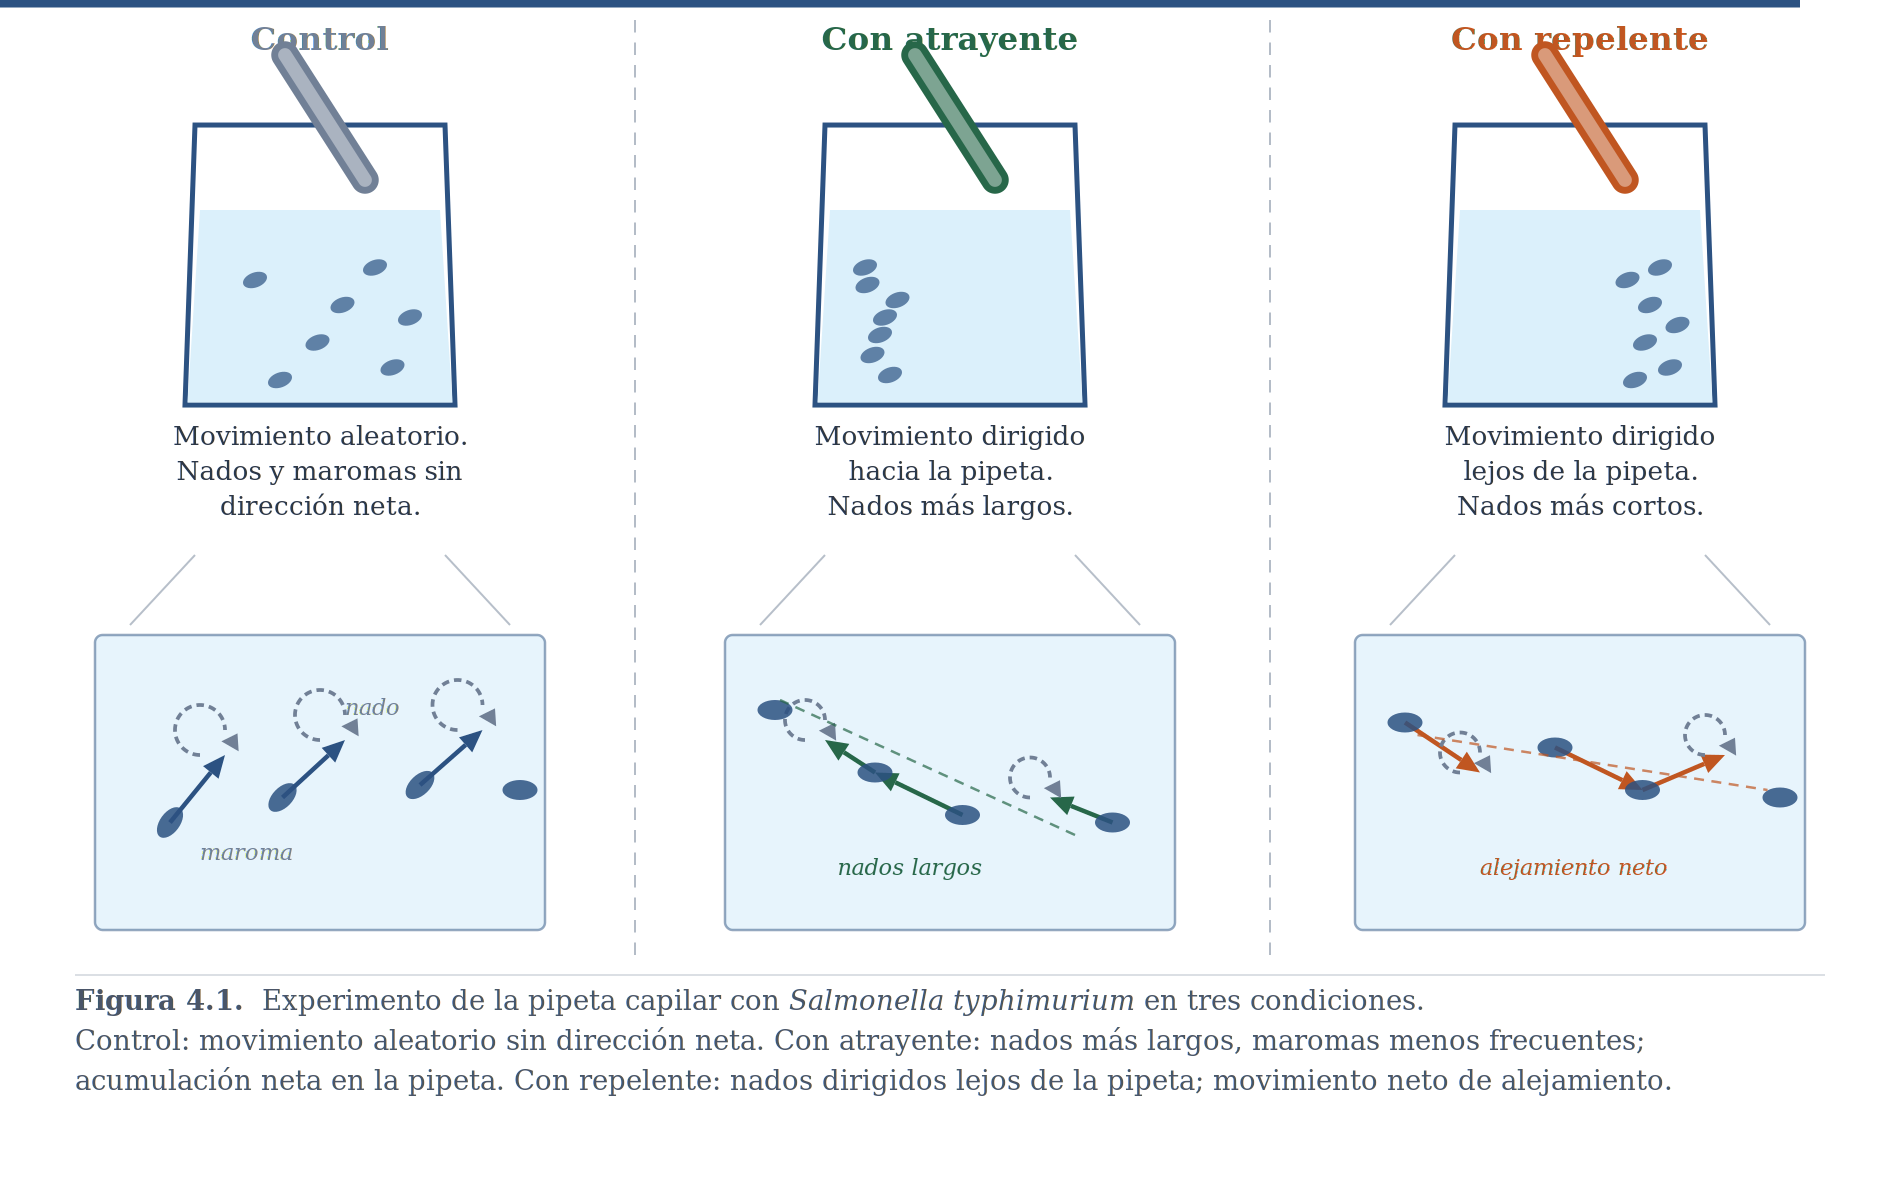
\includegraphics[width=7.8125in,height=\textheight,keepaspectratio]{Figuras/fig4_1_pipeta_capilar.png}

}

\caption{\label{fig-pipeta-capilar}}

\end{figure}%

La observación detallada del movimiento de salmonelas individuales
revela dos comportamientos básicos que se alternan. El primero son las
\textbf{maromas} (\emph{tumbling mode}): la bacteria gira sobre sí misma
sin desplazamiento neto ---exploración, muestreo de diferentes
direcciones posibles. El segundo es el \textbf{nado en línea recta}
(\emph{running mode}): la bacteria avanza en la dirección actual
---explotación de una dirección prometedora. La
Fig.~\ref{fig-modos_locomocion} muestra el mecanismo físico: en modo
maroma, los flagelos rotan en sentido horario y se desenredan; en nado
recto, rotan en sentido antihorario y forman un haz sincronizado que
propulsa a la bacteria.

\begin{figure}

\centering{

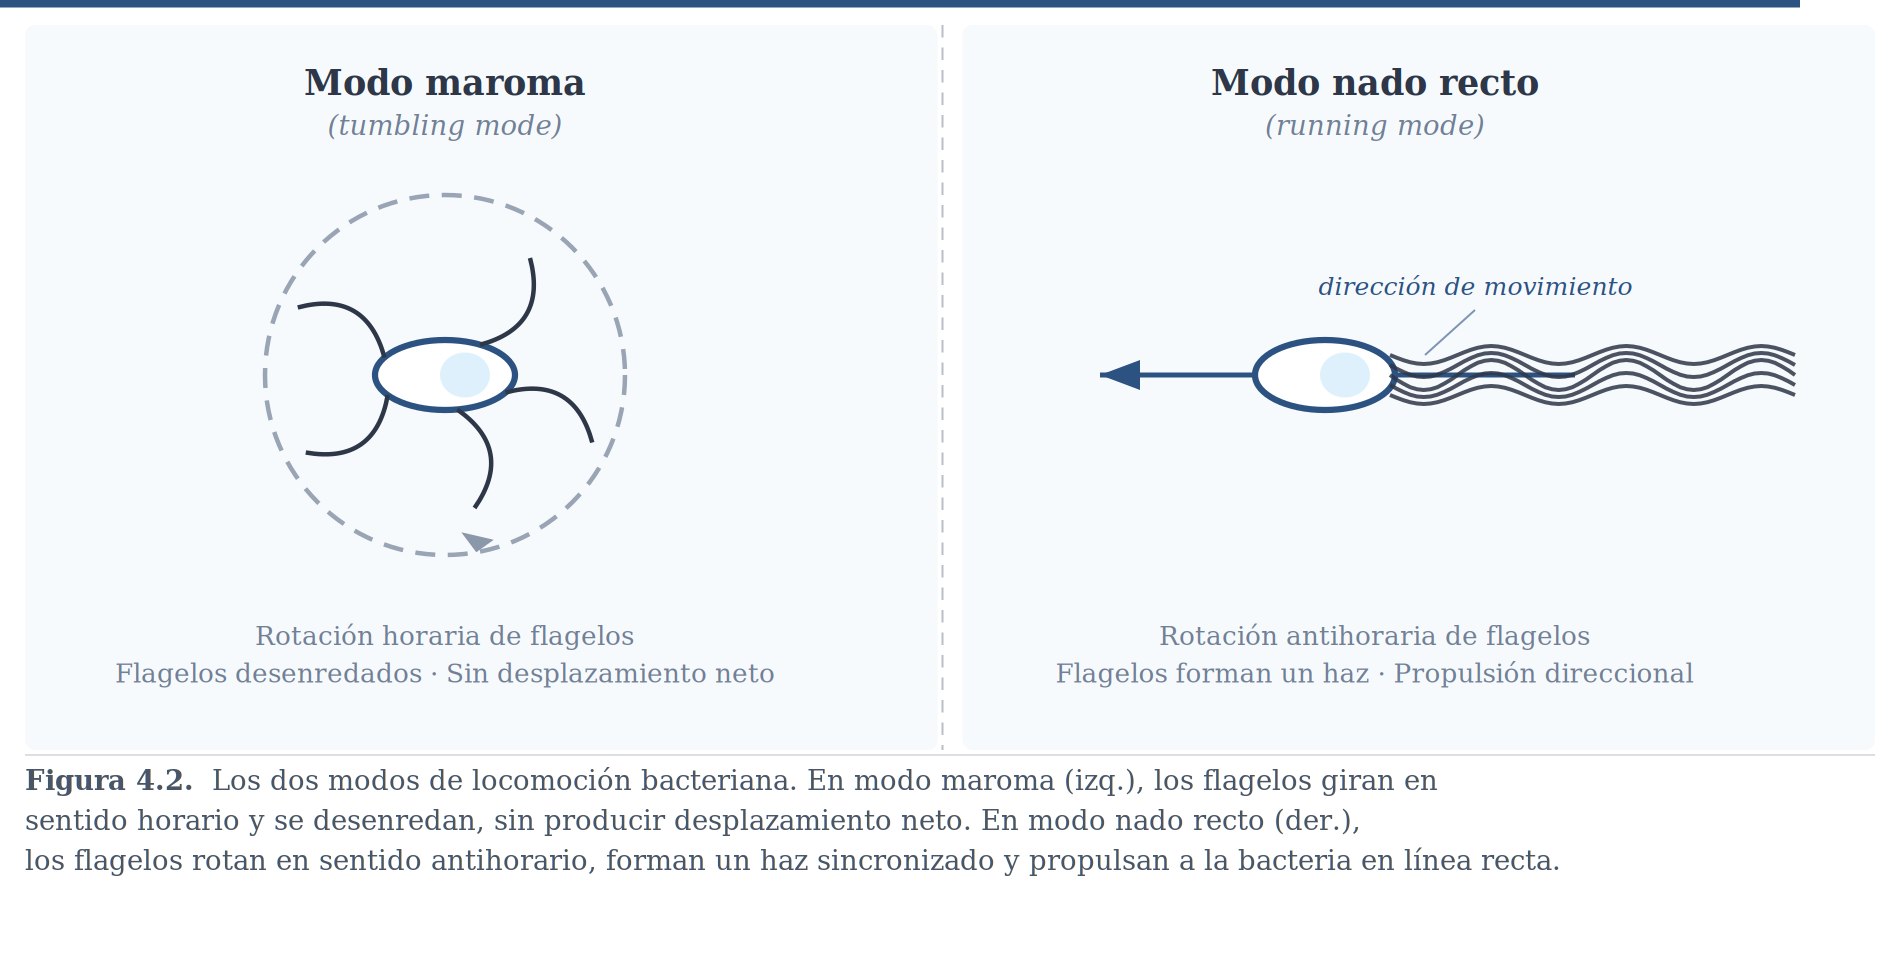
\includegraphics[width=7.8125in,height=\textheight,keepaspectratio]{Figuras/fig4_2_modos_locomocion.png}

}

\caption{\label{fig-modos_locomocion}}

\end{figure}%

Lo crucial no son los dos comportamientos en sí, sino la regla que
determina cuándo cambiar de uno a otro: si la concentración química está
mejorando, continúa el nado recto; si deja de mejorar o empeora, pasa a
maromas hasta que por casualidad apunte en una dirección donde la
concentración vuelva a mejorar. Lo que controla la transición no son los
valores absolutos de concentración, sino los \emph{cambios}. La bacteria
es sensible a si las cosas están mejorando o empeorando, no a cuán
buenas son en un momento dado.

\subsection{La Pregunta Crucial: ¿Simultánea o
Sucesiva?}\label{la-pregunta-crucial-simultuxe1nea-o-sucesiva}

Esto nos lleva a una pregunta fundamental: ¿cómo ``sabe'' la bacteria si
va en la dirección correcta? Hay dos posibilidades en principio. La
primera es \textbf{comparación simultánea}: la bacteria podría tener
receptores en diferentes partes de su cuerpo que comparan la
concentración en distintos puntos del espacio al mismo tiempo, como un
mamífero que compara las señales que llegan a sus dos fosas nasales. La
segunda es \textbf{comparación sucesiva}: la bacteria compara la
concentración en su posición actual con la concentración en su posición
inmediatamente anterior.

La evidencia experimental descarta la primera posibilidad. El diámetro
de una bacteria es tan pequeño que la diferencia de concentración entre
sus dos extremos es prácticamente imperceptible ---el gradiente
espacial, a esa escala, no puede detectarse. Lo que sí puede detectarse
son los \emph{cambios temporales} en la concentración mientras la
bacteria se mueve. Esto se confirma experimentalmente: las transiciones
entre maromas y nado recto se producen ante cambios bruscos en la
concentración, no ante valores absolutos. Como veremos a lo largo del
curso, esta sensibilidad a cambios más que a valores absolutos es una
característica ubicua de los sistemas sensoriales y de aprendizaje.

\subsection{La Adaptación Sensorial}\label{la-adaptaciuxf3n-sensorial}

Hay una complicación adicional. Si la bacteria cambiara a nado recto
ante el primer incremento detectado y se quedara así indefinidamente,
probablemente terminaría en la primera mejora que encontró, no en la
mejor ubicación posible. Las bacterias resuelven esto mediante
\textbf{adaptación sensorial}: después de un tiempo breve ---menos de un
minuto en Salmonella--- el sistema de detección ``se acostumbra'' al
nivel actual de concentración. Lo que antes parecía ``alta
concentración'' se convierte gradualmente en el nuevo punto de
referencia ``normal''. La bacteria vuelve a dar maromas hasta encontrar
una concentración aún mayor.

La Fig.~\ref{fig-respuesta_atrayente} muestra esta dinámica
cuantitativamente. Cuando se añade un atrayente en t = 0, la fracción de
bacterias en nado recto aumenta abruptamente, reflejando el cambio
brusco detectado. Pero en el transcurso de menos de un minuto esa
fracción regresa a los valores basales, aun cuando el atrayente sigue
presente: la adaptación sensorial ajustó el punto de referencia al nuevo
nivel. El sistema vuelve a ser sensible a \emph{cambios adicionales}.

\begin{figure}

\centering{

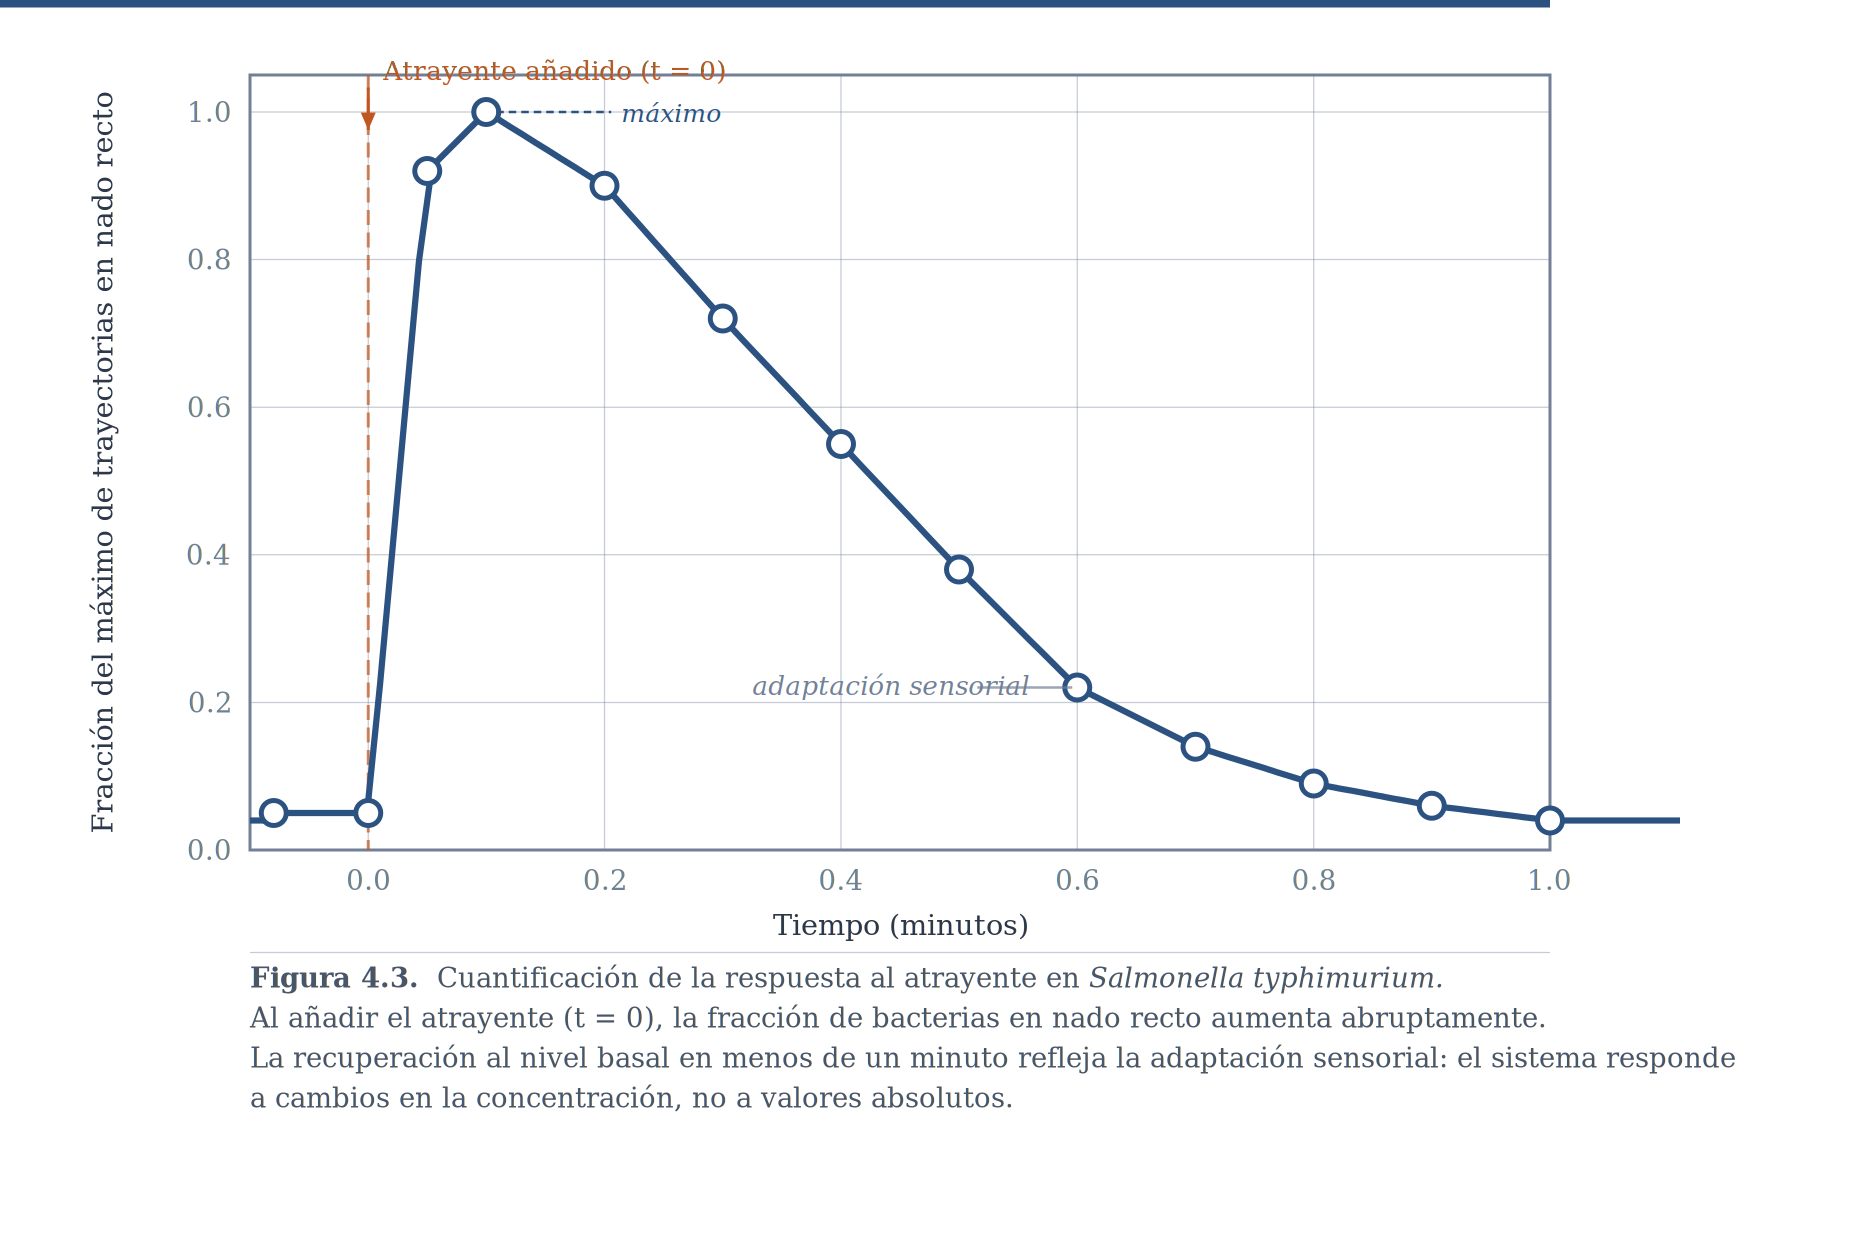
\includegraphics[width=7.8125in,height=\textheight,keepaspectratio]{Figuras/fig4_3_respuesta_atrayente.png}

}

\caption{\label{fig-respuesta_atrayente}}

\end{figure}%

La adaptación sensorial implementa una forma de insatisfacción
adaptativa: el organismo nunca se contenta completamente con lo actual,
sino que sigue buscando mientras haya tiempo y energía. Como veremos más
adelante, esta misma lógica reaparece en mecanismos de aprendizaje mucho
más complejos.

\section{El Algoritmo}\label{el-algoritmo}

Imagina que subes el Ajusco con los ojos vendados. No puedes ver la cima
ni el sendero. Lo único que puedes hacer es sentir si el suelo bajo tus
pies va hacia arriba o hacia abajo. Si sube, sigues en esa dirección. Si
empieza a bajar, te detienes y tanteas otras direcciones hasta encontrar
una que vuelva a subir. Después de un tiempo ---aunque la cuesta siga
siendo empinada--- el esfuerzo muscular se vuelve la nueva normalidad y
ya no distingues si estás subiendo o no: vuelves a tantear. Eso es todo
el algoritmo. La bacteria hace exactamente lo mismo, pero con
concentración química en lugar de pendiente, y con flagelos en lugar de
piernas.

El mecanismo necesita las mismas piezas en cualquier implementación: un
sensor que detecta cambios en la variable relevante, una memoria
brevísima del momento anterior, dos modos de movimiento contrastantes
---explorar y explotar---, una regla para cambiar entre ellos, y la
adaptación sensorial que equivale al momento en que dejas de sentir la
pendiente y te obliga a buscar de nuevo. Con esas cinco piezas, el
algoritmo está completo.

Existe además una variante ligeramente más sofisticada: en lugar de
tomar la primera dirección que mejore, el organismo muestrea múltiples
direcciones, registra el valor en cada una, y se mueve hacia la que
mostró la mayor mejora. Es el \textbf{ascenso de mayor pendiente} ---más
costoso en memoria, pero más eficiente en entornos ruidosos donde un
solo muestreo puede dar una impresión equivocada. El ejemplo de wifi lo
ilustra bien: en la versión simple das un paso en una dirección y
decides; en la versión de mayor pendiente te detienes, exploras varios
pasos en distintas direcciones, memorizas los valores, y luego caminas
decididamente hacia donde la señal fue mayor.

En ambos casos estás haciendo \emph{comparaciones sucesivas}, igual que
la bacteria: no puedes ver el router, solo puedes comparar si tienes más
o menos señal que hace un momento. Esto distingue al ascenso de colina
del mecanismo que veremos en el capítulo siguiente, donde la comparación
es simultánea ---dos puntos del espacio se comparan al mismo tiempo, no
el mismo punto en dos momentos distintos.

\textbf{¿Qué tan bueno es el algoritmo?}

El algoritmo que describimos funciona, pero conviene preguntarse qué tan
bien funciona y si puede hacerse mejor. Para eso, la competencia del
Ajusco es útil más allá de ilustrar el mecanismo.

Imagina que ahora tienes información sobre la montaña: sabes que el
Ajusco no es una colina perfectamente suave sino un terreno accidentado,
con peñascos, cerros secundarios y mesetas que desde abajo parecen la
cima. Tu compañero está vendado y usa el ascenso simple ---da un paso,
siente si subió o bajó, decide. Tú también estás vendado, pero usas el
ascenso de mayor pendiente: antes de comprometerte con una dirección,
tanteas varios pasos en distintas direcciones, memorizas los valores, y
luego avanzas decididamente hacia donde la pendiente fue mayor. En una
montaña suave, tu estrategia no te da ninguna ventaja y te cuesta tiempo
extra. En una montaña con muchos cerros secundarios, tu estrategia
reduce el riesgo de quedarte atascado en uno de ellos.

Pero hay algo que ambos hacen mal: el tamaño del paso. Lejos de la cima,
cuando el terreno cambia rápidamente con cada movimiento, tiene sentido
dar pasos grandes ---la información de un paso pequeño es poco
informativa respecto a si la dirección general es buena. Conforme te
acercas a la cima, la pendiente se suaviza y la señal de cada paso se
vuelve más pequeña y más ruidosa. En ese momento, un paso grande puede
hacerte cruzar la cima sin notarlo. El paso óptimo no es constante: debe
ir reduciéndose conforme se acerca al objetivo.

En la ecuación del mecanismo, el tamaño efectivo del paso está
controlado por el parámetro \emph{b}: cuánto peso le da el sistema a
cada diferencia detectada. Un \emph{b} grande actúa como un paso largo
---sensible, rápido para reaccionar, pero propenso a sobrepasar el
objetivo. Un \emph{b} pequeño actúa como un paso corto ---robusto ante
el ruido, pero lento para reaccionar ante cambios reales. El valor
óptimo de \emph{b} no es fijo: depende de las características del
terreno que está navegando el organismo.

Lo mismo aplica al parámetro \emph{a}, que controla cuánto tiempo sigue
el organismo en modo de explotación después de que la señal se
estabiliza. En una montaña con pocos máximos locales, un \emph{a} alto
es bueno ---el organismo explota con inercia y llega rápido a la cima.
En una montaña con muchos cerros secundarios, un \emph{a} alto es una
trampa: el inercia del sistema lo mantiene escalando el primer cerro que
encuentra aunque haya uno más alto a su izquierda. El valor óptimo de
\emph{a} también depende del terreno.

Esto no es un defecto del mecanismo sino una propiedad fundamental de
cualquier algoritmo de búsqueda: no existe una estrategia universalmente
óptima independiente del problema. Lo que existe son estrategias bien
adaptadas a tipos particulares de entornos. Y si el entorno cambia, o si
el organismo no sabe de antemano qué tipo de entorno enfrenta, el valor
fijo de \emph{a} y \emph{b} con que parte puede ser bueno o puede ser
desastroso.

La solución verdaderamente óptima al problema no es encontrar los
mejores valores fijos de \emph{a} y \emph{b}, sino desarrollar la
capacidad de \emph{ajustar esos valores conforme se acumula experiencia
con el entorno}. Un agente que empieza con pasos grandes cuando el
terreno es desconocido y los va reduciendo sistemáticamente conforme
aprende que está cerca de un óptimo ---ese agente es mejor que cualquier
agente con parámetros fijos, sin importar qué tan bien calibrados estén
esos parámetros. Esa capacidad de ajustar adaptativamente la importancia
del error es exactamente lo que veremos en los mecanismos de aprendizaje
de los bloques siguientes.

Veremos esa capacidad ---ajustar adaptativamente la importancia del
cambio detectado--- cuando lleguemos a los modelos de aprendizaje
asociativo en el Bloque II.

\section{Formalización Matemática}\label{formalizaciuxf3n-matemuxe1tica}

En el simulador que acaban de explorar, el parámetro \emph{a} es
exactamente el tiempo que el agente sigue explotando después de que la
concentración dejó de mejorar. Con \emph{a} cercano a 1, la inercia es
grande ---como un corredor que tarda en frenar. Con \emph{a} cercano a
0, para casi de inmediato. El término \emph{b·{[}X(t+1) − X(t){]}} es la
diferencia que ya calcularon en los ejercicios del simulador,
multiplicada por qué tanto le importa al sistema esa diferencia.

Juntando las dos partes, la ecuación que rige todo lo que observaron es:

\[Y(t+1) = a \cdot Y(t) + b \cdot [X(t+1) - X(t)]\]

donde Y(t) es la variable de decisión que determina el modo conductual,
X(t) es el valor de la variable ambiental (concentración química,
intensidad lumínica, señal de wifi), \emph{a} es el parámetro de
adaptación sensorial (0 \textless{} a \textless{} 1), y \emph{b} es el
parámetro de sensibilidad al cambio (b \textgreater{} 0).

La regla de respuesta conecta Y con el comportamiento observable: si Y
supera un umbral (típicamente cero), el organismo explota ---nado recto,
crecimiento hacia la luz, caminar en esa dirección; si Y está por
debajo, explora ---maromas, rotación, prueba otra dirección.

El marciano del capítulo anterior se preguntaba qué \emph{hace} el
vehículo. Aquí la pregunta es qué \emph{problema resuelve} la bacteria
---y esa pregunta nos dice por qué la ecuación tiene la forma que tiene.
Si el problema es navegar sin mapa y sin receptores de distancia,
necesitas comparación temporal, no espacial. Y necesitas adaptación que
te impida conformarte con el primer gradiente positivo que encuentres.
Todo lo demás se sigue de ahí.

\subsection{Un Ejemplo Numérico}\label{un-ejemplo-numuxe9rico}

Sigamos la dinámica con valores concretos: a = 0.9, b = 0.5, umbral = 0.
Partimos de Y(0) = 0 y X(0) = 5. El agente está en modo exploración.

\textbf{Tiempo 1:} X(1) = 7 --- la concentración mejora. Y(1) = 0.9 × 0
+ 0.5 × (7 − 5) = 0 + 1.0 = \textbf{1.0} → Explotar.

\textbf{Tiempo 2:} X(2) = 9 --- sigue mejorando. Y(2) = 0.9 × 1.0 + 0.5
× (9 − 7) = 0.9 + 1.0 = \textbf{1.9} → Explotar.

\textbf{Tiempo 3:} X(3) = 9 --- la concentración se estabiliza. Y(3) =
0.9 × 1.9 + 0.5 × (9 − 9) = 1.71 + 0 = \textbf{1.71} → Explotar (Y
empieza a decaer).

\textbf{Tiempo 4:} X(4) = 8 --- baja ligeramente. Y(4) = 0.9 × 1.71 +
0.5 × (8 − 9) = 1.54 − 0.5 = \textbf{1.04} → Explotar.

\textbf{Tiempo 5:} X(5) = 7 --- sigue bajando. Y(5) = 0.9 × 1.04 + 0.5 ×
(7 − 8) = 0.94 − 0.5 = \textbf{0.44} → Explotar (Y casi en umbral).

\textbf{Tiempo 6:} X(6) = 6 --- sigue empeorando. Y(6) = 0.9 × 0.44 +
0.5 × (6 − 7) = 0.40 − 0.5 = \textbf{−0.10} → \textbf{Explorar}.

La secuencia muestra algo importante: el sistema no cambia a exploración
en el instante en que la concentración deja de mejorar. La inercia del
término a·Y mantiene la explotación durante un tiempo ---un filtro que
evita responder a fluctuaciones momentáneas. Pero si la concentración no
mejora de forma sostenida, Y cae por debajo del umbral y el organismo
vuelve a buscar. Esto corresponde exactamente a lo que muestra la figura
4.3: la bacteria mantiene el nado recto por un tiempo incluso cuando la
concentración se estabiliza, antes de que la adaptación sensorial la
devuelva al modo exploración.

\begin{tcolorbox}[enhanced jigsaw, arc=.35mm, bottomrule=.15mm, bottomtitle=1mm, breakable, colback=white, colbacktitle=quarto-callout-tip-color!10!white, colframe=quarto-callout-tip-color-frame, coltitle=black, left=2mm, leftrule=.75mm, opacityback=0, opacitybacktitle=0.6, rightrule=.15mm, title=\textcolor{quarto-callout-tip-color}{\faLightbulb}\hspace{0.5em}{🕹️ ¡Prueba el Simulador Interactivo!}, titlerule=0mm, toprule=.15mm, toptitle=1mm]

Para explorar los conceptos de este capítulo en la práctica, abre el
siguiente simulador:

\href{https://colab.research.google.com/github/arbouria/Libro-ACA-2026/blob/main/Simuladores/ascenso_colina.ipynb}{\textbf{Abrir
Simuladores en Google Colab}}

\end{tcolorbox}

Verás un agente navegando un paisaje de concentración con dos fuentes:
una fuente principal (la meta) y un máximo local (la trampa).
Parámetros: \emph{a}, \emph{b}, nivel de ruido. La trayectoria se
colorea por modo: exploración en azul, explotación en naranja. Gráficas
en tiempo real de Y(t) y X(t).

\textbf{Objetivo:} Descubrir qué combinación de adaptación sensorial y
sensibilidad al cambio produce navegación eficiente, y por qué ninguno
de los extremos funciona bien.

\emph{Básico:} Comienza con a = 0.9 y b = 0.5. Antes de iniciar la
simulación, predice: ¿crees que el agente llegará a la fuente principal
o quedará atrapado en el máximo local? Corre la simulación y verifica.
Ahora reduce a a 0.3 manteniendo b constante. ¿Qué cambia?

\emph{Intermedio:} Con a = 0.97 (adaptación muy lenta), ¿el agente
escapa del máximo local? Prueba a = 0.5. ¿Por qué la adaptación
sensorial ayuda a escapar de los máximos locales? Piensa en términos del
Ajusco: si nunca dejas de sentir la pendiente actual, ¿qué te impide
buscar una pendiente mayor?

\emph{Avanzado:} Activa el ruido ambiental. Encuentra la combinación de
a y b que produce la navegación más eficiente con ruido alto. ¿Por qué
algunos valores de b que funcionaban sin ruido ya no funcionan? ¿Qué
hace que el ruido sea un problema para la sensibilidad al cambio?

\section{Lo que el Ascenso de Colina Hace y No
Hace}\label{lo-que-el-ascenso-de-colina-hace-y-no-hace}

El ascenso de colina permite adaptación en tiempo real y navegación
eficiente hacia gradientes sin mapa ni receptores de distancia. El
balance exploración-explotación emerge automáticamente de la dinámica
del sistema, y la inercia del término a·Y actúa como filtro ante el
ruido.

Lo que el mecanismo \emph{no} hace es igualmente revelador. En este
modelo la comparación es entre el valor actual y el valor inmediatamente
anterior: \textbf{no hay integración de experiencias pasadas}. Si
repetimos la misma situación mañana, el organismo responde igual que hoy
---no hay memoria de largo plazo. El mecanismo es puramente reactivo:
responde a cambios que ya ocurrieron, no anticipa cambios futuros. No
hay modelo interno del entorno ni representación de dónde están las
fuentes. Y no hay aprendizaje en el sentido estricto: una bacteria que
navegó exitosamente ayer no navega mejor hoy por haber tenido esa
experiencia.

Esta distinción es central para el libro. El \textbf{comportamiento
adaptativo sin aprendizaje} ---como el ascenso de colina--- produce
flexibilidad conductual en respuesta al entorno actual, pero sin retener
información de experiencias previas. El \textbf{comportamiento
adaptable} ---que estudiaremos en los bloques siguientes--- supone
exactamente eso: un cambio duradero en el sistema como resultado de la
experiencia. El ascenso de colina es un mecanismo sin historia. Su
importancia pedagógica está en que los mismos principios ---comparación,
reducción de error, balance exploración-explotación--- reaparecerán,
transformados y enriquecidos, en los mecanismos de aprendizaje que
estudiaremos más adelante.

\section{Conexiones}\label{conexiones}

\subsection{Hacia atrás: Selección
Natural}\label{hacia-atruxe1s-selecciuxf3n-natural}

El ascenso de colina es una instancia de ensayo y error análoga, en su
lógica, a la selección natural: la exploración aleatoria genera
variación conductual; la comparación determina qué variantes se
explotan; la explotación continúa mientras el gradiente es favorable. La
diferencia crucial es la escala temporal. La selección natural opera en
generaciones; el ascenso de colina opera en segundos o minutos en la
vida del individuo. Son el mismo principio en escalas de tiempo
radicalmente distintas.

\subsection{Hacia adelante: Aprendizaje por
Refuerzo}\label{hacia-adelante-aprendizaje-por-refuerzo}

La diferencia {[}X(t+1) − X(t){]} es una primera versión del
\textbf{error de predicción}: la discrepancia entre lo que se esperaba y
lo que ocurrió. La actualización incremental de Y es análoga a cómo el
valor asociativo se ajusta ensayo a ensayo en los modelos del Bloque II.
Y el dilema exploración-explotación, que aquí aparece en su forma más
simple, se convertirá en uno de los problemas centrales del aprendizaje
por refuerzo en el Bloque IV.

\subsection{Lateral: Sistemas de Retroalimentación (Próximo
Capítulo)}\label{lateral-sistemas-de-retroalimentaciuxf3n-pruxf3ximo-capuxedtulo}

El ascenso de colina utiliza \textbf{comparación sucesiva}: el mismo
lugar en dos momentos distintos. El próximo capítulo introduce los
sistemas de retroalimentación, que utilizan \textbf{comparación
simultánea}: dos puntos del espacio se comparan al mismo tiempo. Ambos
son mecanismos de adaptación sin aprendizaje, pero la diferencia en el
tipo de comparación tiene consecuencias importantes para qué problemas
puede resolver cada uno ---y la distinción entre los dos es exactamente
lo que la evidencia experimental descartó en la Salmonella.

\bookmarksetup{startatroot}

\chapter{Resumen}\label{resumen-1}

El problema adaptativo de este capítulo es localizar recursos en
entornos variables sin receptores de distancia ni mapa previo. La
solución es el ascenso de colina: un algoritmo de comparación sucesiva
que alterna entre exploración aleatoria y explotación direccional,
guiado por cambios en una variable ambiental de interés. Sus piezas
esenciales son: un sensor de cambios, una memoria mínima del momento
anterior, dos modos conductuales contrastantes, una regla de transición
entre ellos, y adaptación sensorial que previene el estancamiento en
máximos locales.

Lo que el mecanismo no hace es tan importante como lo que hace: no hay
integración de historia, ni predicción, ni representación del entorno,
ni cambio duradero. Es comportamiento adaptativo sin aprendizaje. Su
relevancia pedagógica está en que los mismos principios ---comparación,
reducción de error, balance exploración-explotación--- reaparecerán,
transformados y enriquecidos, en los mecanismos de aprendizaje de los
bloques siguientes.

\section{Ejercicios de
Comprensión}\label{ejercicios-de-comprensiuxf3n-1}

\textbf{1.} La figura 4.3 muestra que después de añadir un atrayente, la
fracción de bacterias en nado recto aumenta abruptamente y luego regresa
a los valores basales en menos de un minuto. Explica este patrón en
términos del parámetro \emph{a} de la ecuación. ¿Qué valor de \emph{a}
produciría una recuperación más rápida? ¿Qué pasaría si \emph{a} = 1
exactamente?

\textbf{2.} El capítulo descarta la posibilidad de comparación
simultánea en Salmonella con un argumento basado en el tamaño de la
bacteria. Formula ese argumento con tus propias palabras. ¿Puedes pensar
en algún organismo que sí pudiera usar comparación simultánea para
detectar un gradiente químico?

\textbf{3.} Imagina que buscas señal de wifi en un edificio desconocido.
Describe, paso a paso, cómo aplicarías el ascenso de mayor pendiente.
¿En qué situaciones preferirías el ascenso simple? ¿Cuándo valdría la
pena el esfuerzo adicional?

\textbf{4.} Usando la ecuación Y(t+1) = a·Y(t) + b·{[}X(t+1) − X(t){]},
con a = 0.8 y b = 1.0, completa la tabla. El umbral para explotar es 0.

{\def\LTcaptype{none} % do not increment counter
\begin{longtable}[]{@{}llll@{}}
\toprule\noalign{}
t & X(t) & Y(t) & ¿Explorar o explotar? \\
\midrule\noalign{}
\endhead
\bottomrule\noalign{}
\endlastfoot
0 & 10 & 0 & --- \\
1 & 12 & ? & ? \\
2 & 14 & ? & ? \\
3 & 14 & ? & ? \\
4 & 13 & ? & ? \\
\end{longtable}
}

¿En qué momento el sistema cambia de modo? ¿Qué dice eso sobre la
relación entre estabilización de concentración y exploración?

\textbf{5.} El capítulo afirma que el ascenso de colina no es
aprendizaje. ¿Qué le falta para serlo? Formula una modificación
hipotética al mecanismo que lo convertiría en algo más parecido al
aprendizaje. ¿Qué nueva capacidad adaptativa tendría el organismo con
esa modificación?

\textbf{6.} \emph{(Reflexión)} La adaptación sensorial implementa una
forma de ``insatisfacción adaptativa''. ¿Por qué sería desadaptativo un
organismo que no tuviera esta propiedad ---que se contentara para
siempre con el primer gradiente positivo que encontrara? ¿Puedes pensar
en algún contexto donde esa estrategia podría ser ventajosa?

\bookmarksetup{startatroot}

\chapter{Sistemas de
Retroalimentación}\label{sistemas-de-retroalimentaciuxf3n}

\section{Comparación Simultánea y el Límite de la
Reactividad}\label{comparaciuxf3n-simultuxe1nea-y-el-luxedmite-de-la-reactividad}

En el capítulo anterior dejamos a la bacteria navegando con un solo
sensor. Su estrategia era comparar \emph{ahora} con \emph{hace un
momento} en el mismo lugar: si la concentración mejora, sigue; si
empeora, busca otra dirección. Eso funciona, pero es lento y sinuoso. La
bacteria no sabe hacia dónde está el nutriente ---solo sabe si está
mejorando o no.

La aparición de la simetría bilateral en los animales resolvió esa
limitación de una forma elegante: en lugar de un sensor que se mueve
para comparar el mundo en distintos tiempos, el organismo dispone de dos
sensores separados que comparan el mundo en distintos lugares \emph{al
mismo tiempo}. Con este arreglo, la dirección de la fuente queda
codificada directamente en la diferencia entre lo que detecta el lado
izquierdo y lo que detecta el lado derecho, sin necesidad de moverse
primero para saberlo.

Este capítulo introduce el mecanismo que hace posible esa comparación
simultánea y lo generaliza: el \textbf{sistema de retroalimentación}.
Veremos cómo está organizado, qué preguntas conviene hacerle, y ---lo
más importante--- cuál es la limitación fundamental que comparte con el
ascenso de colina y que abre la puerta al aprendizaje.

\section{El Problema: Orientarse en el
Espacio}\label{el-problema-orientarse-en-el-espacio}

Imagina a una polilla nocturna. Hay una fuente de luz a una distancia
desconocida. No tiene mapa, no tiene brújula. Solo tiene lo que sus dos
ojos detectan en este momento: dos intensidades luminosas, una para cada
lado de su cuerpo. ¿Cómo usa esa información mínima para orientar su
cuerpo hacia la fuente?

Este problema ---orientarse hacia o alejarse de una fuente puntual de
estimulación--- aparece en múltiples modalidades a lo largo del reino
animal. La fototaxia de polillas y cucarachas, la quimiotaxia de
insectos siguiendo plumas de feromonas, la fonotaxia de grillos hembra
localizando machos que cantan, la termotaxia de serpientes detectando
presas de sangre caliente: todos son el mismo problema computacional
resuelto con el mismo principio básico. La diversidad está en el tipo de
estímulo; el mecanismo subyacente es el mismo.

\section{El Mecanismo: Comparación
Simultánea}\label{el-mecanismo-comparaciuxf3n-simultuxe1nea}

La solución más simple posible al problema de orientación tiene dos
componentes. Primero, comparar simultáneamente la estimulación que llega
al receptor izquierdo con la que llega al derecho. Segundo, girar en la
dirección del receptor que recibe más estimulación ---en el caso de
fototaxia positiva, hacia la luz; en el caso de fototaxia negativa, como
la cucaracha, en dirección contraria.

Este mecanismo ---conocido en biología como \textbf{tropotaxia}--- es
una instancia del principio más general que introduce este capítulo: el
\textbf{sistema de retroalimentación}. La información direccional está
disponible instantáneamente, sin costo de movimiento. No hay que
explorar para saber hacia dónde girar.

Dos experimentos clásicos establecen que lo que controla el
comportamiento es la \emph{diferencia} entre sensores, no el nivel
absoluto de estimulación en ninguno de ellos.

El primero cubre uno de los ojos compuestos de una polilla con pintura
opaca. La predicción es directa: con solo un sensor funcional, la
diferencia bilateral siempre favorece ese lado; la señal de corrección
nunca se cancela porque no hay información desde el lado opuesto. El
resultado es un giro continuo, sin orientación hacia ningún punto.
Cuando se cubre el ojo izquierdo, la polilla gira continuamente a la
izquierda; cuando se cubre el derecho, gira a la derecha. La cucaracha
hace exactamente lo opuesto ---porque huye de la luz--- lo que confirma
que el signo del giro depende del tipo de fototaxia, no de cuál ojo está
disponible.

\begin{figure}

{\centering 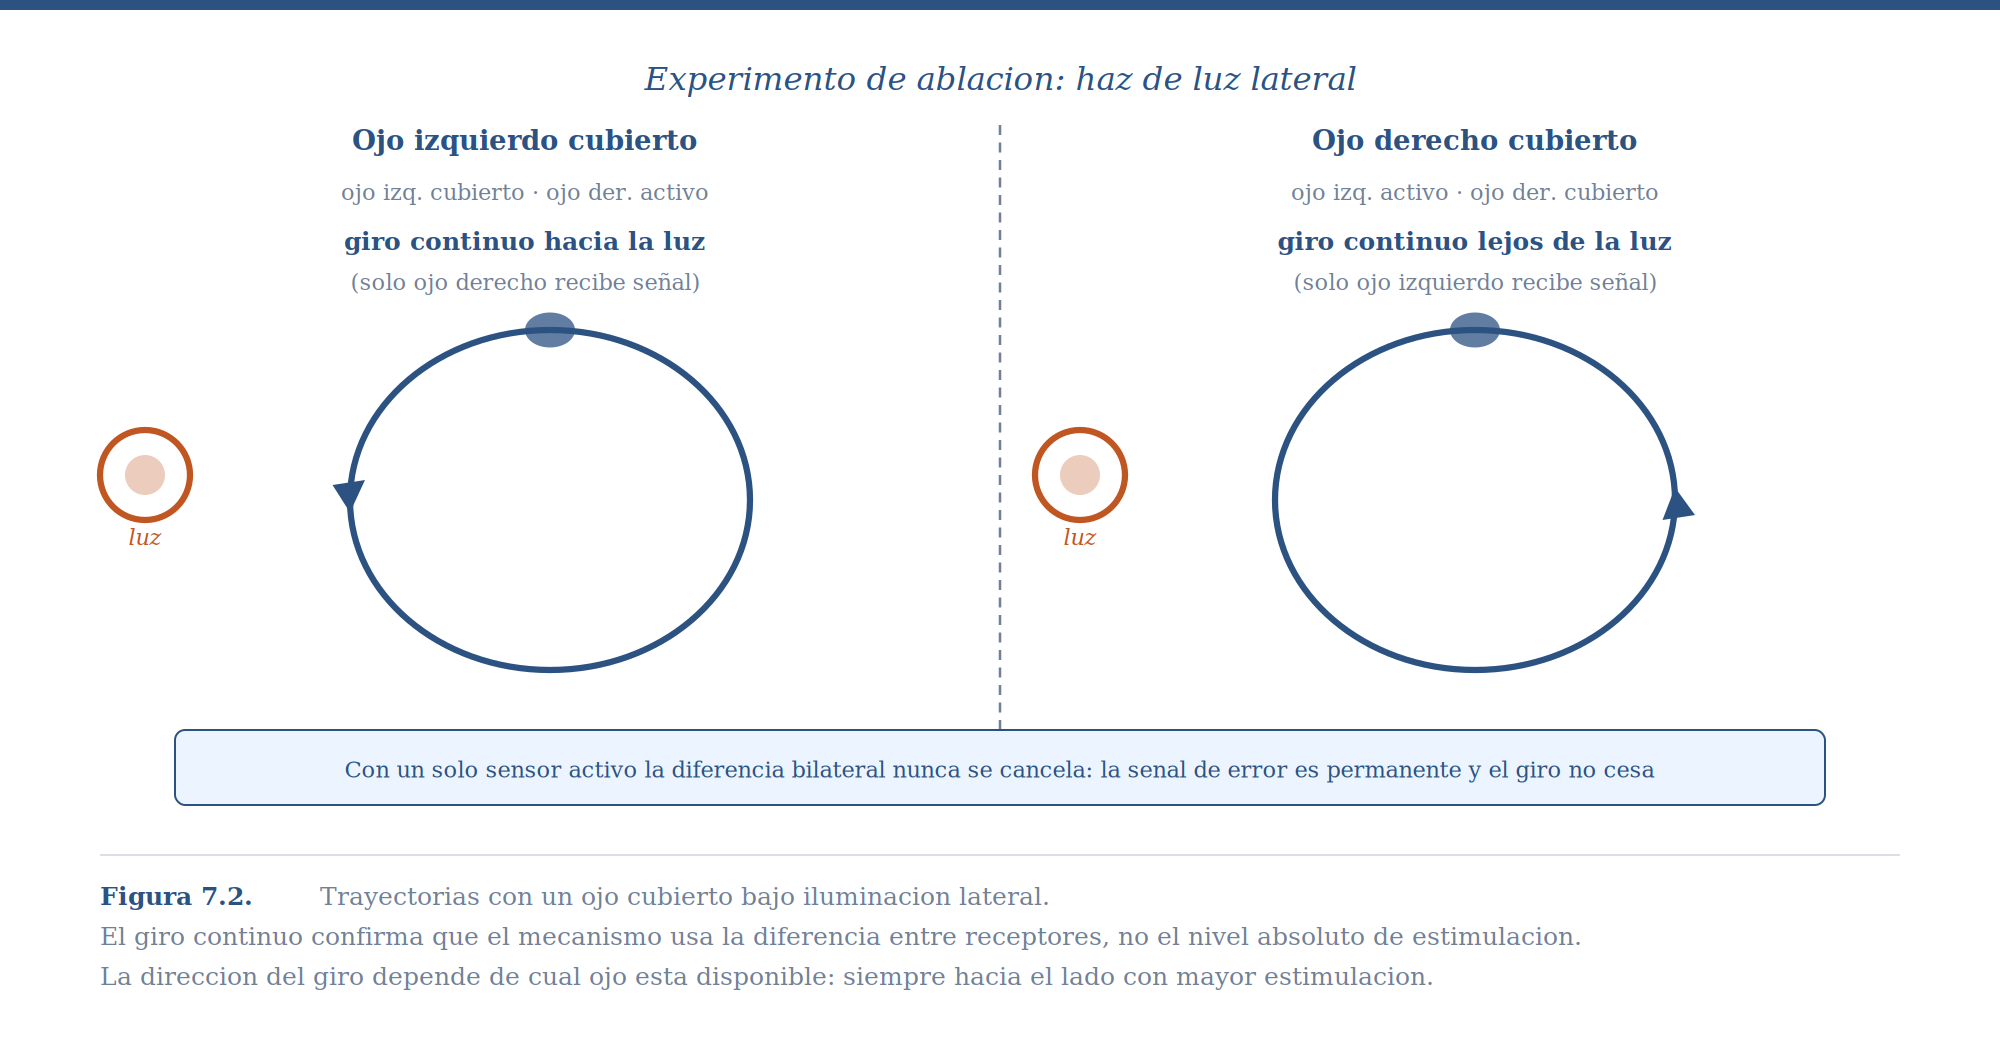
\includegraphics[width=7.8125in,height=\textheight,keepaspectratio]{Figuras/fig7_2_ojo_cubierto.png}

}

\caption{Trayectorias con un ojo cubierto}

\end{figure}%

\begin{tcolorbox}[enhanced jigsaw, arc=.35mm, bottomrule=.15mm, breakable, colback=white, colframe=quarto-callout-note-color-frame, left=2mm, leftrule=.75mm, opacityback=0, rightrule=.15mm, toprule=.15mm]

**Descripción:Trayectorias con un ojo cubierto. Filas: oscuridad, luz
arriba, haz de luz. Columnas: ojo izquierdo ciego vs.~ojo derecho ciego.
Con un solo ojo funcional, el organismo gira continuamente en lugar de
orientarse. La dirección del giro depende de qué ojo está disponible y
del tipo de taxia (positiva/negativa).

\end{tcolorbox}

El segundo experimento coloca dos fuentes de luz de igual intensidad a
igual distancia del organismo. Si la conducta está controlada por la
diferencia bilateral, la predicción es que el animal debería moverse en
línea recta entre ambas fuentes ---porque mientras estén equidistantes,
los dos ojos reciben la misma estimulación, la diferencia es cero, y no
hay señal de giro. Eso es exactamente lo que ocurre: el organismo avanza
en línea recta hasta que la proximidad a una de las fuentes rompe la
simetría, momento en que gira bruscamente. Pocas veces un experimento
confirma tan limpiamente una predicción.

\begin{figure}

{\centering 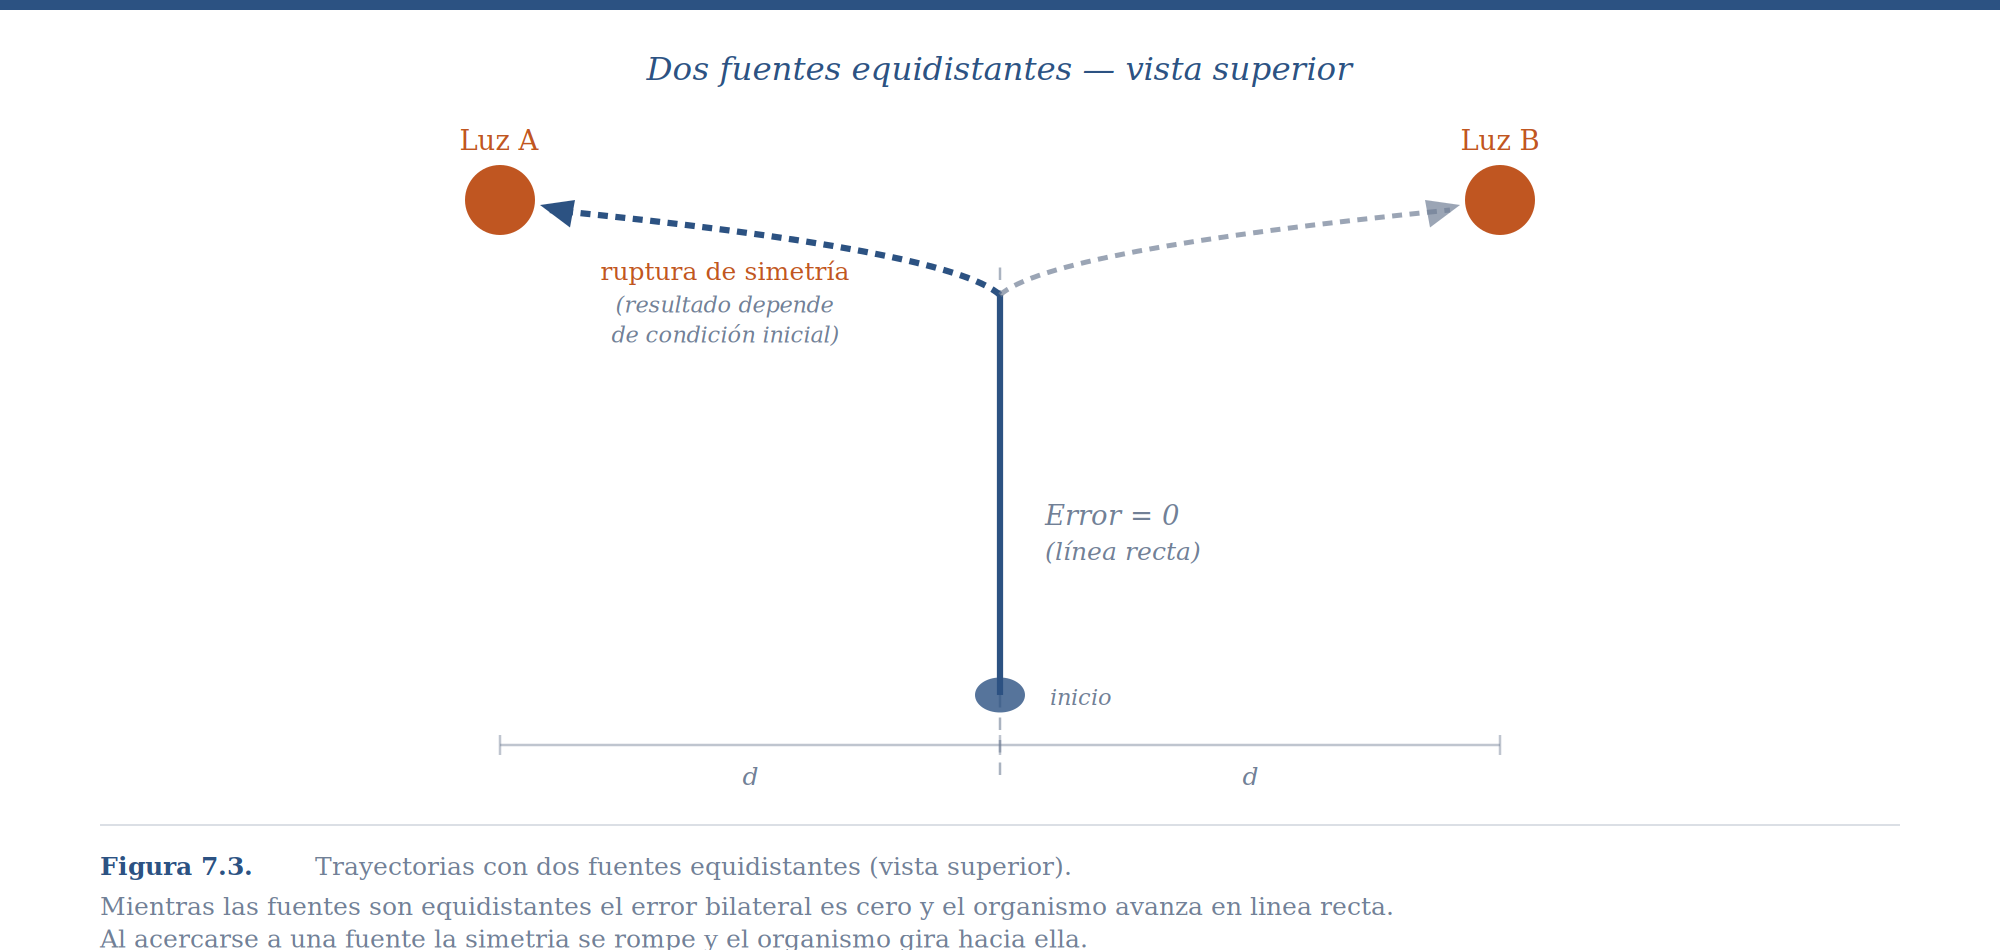
\includegraphics[width=7.8125in,height=\textheight,keepaspectratio]{Figuras/fig7_3_dos_fuentes.png}

}

\caption{Dos fuentes de luz equidistantes}

\end{figure}%

\begin{tcolorbox}[enhanced jigsaw, arc=.35mm, bottomrule=.15mm, breakable, colback=white, colframe=quarto-callout-note-color-frame, left=2mm, leftrule=.75mm, opacityback=0, rightrule=.15mm, toprule=.15mm]

\textbf{Descripción}: Trayectorias de cochinilla con dos fuentes
equidistantes. Las trayectorias reales muestran movimiento en línea
recta entre las dos fuentes y el brusco cambio de dirección al acercarse
a una de ellas. La línea recta ocurre porque la diferencia bilateral es
cero cuando las fuentes son equidistantes.

\end{tcolorbox}

Vale la pena subrayar el contraste con la bacteria del capítulo
anterior: descartamos la comparación simultánea en la Salmonela porque
el organismo es demasiado pequeño para detectar diferencias de
concentración entre sus dos extremos. En la polilla, el tamaño sí
permite esa comparación ---y la evidencia experimental muestra que
exactamente eso es lo que ocurre.

\section{El Sistema de
Retroalimentación}\label{el-sistema-de-retroalimentaciuxf3n}

La fototaxia es un caso particular de un mecanismo general que aparece a
lo largo de la biología y la ingeniería: el \textbf{sistema de
retroalimentación}. Estamos acostumbrados a pensar en la relación
organismo-entorno como unidireccional ---el entorno produce un estímulo,
el organismo produce una respuesta. Pero esa imagen es incompleta: la
respuesta del organismo modifica el entorno, lo que modifica el estímulo
que controla la respuesta.

La temperatura alta produce sudoración; la sudoración reduce la
temperatura; la temperatura reducida disminuye la sudoración. El bebé
recién nacido succiona; la succión extrae leche; la tasa de succión
estimula la producción de leche de la madre. En todos estos casos la
causalidad no va de A a B sino que forma un lazo cerrado donde A y B se
codeterminan mutuamente.

Formalmente, el sistema está definido por dos ecuaciones simultáneas
acopladas. La \textbf{función de control} (del organismo) describe cómo
se transforma el estímulo en comportamiento:

\[C = G(X)\]

La \textbf{función de retroalimentación} (del entorno) describe cómo el
comportamiento modifica el estímulo:

\[X = E(C)\]

En fototaxia: C es la tasa de giro, X es la disparidad bilateral entre
los dos ojos. El giro cambia el ángulo entre el organismo y la fuente,
lo que cambia la disparidad, lo que cambia el giro. El lazo se cierra.

En la implementación biológica concreta hay cuatro componentes
reconocibles. El \textbf{sensor} mide el estado actual ---los ojos
compuestos que detectan intensidad luminosa en cada lado. El
\textbf{comparador} calcula la discrepancia entre el estado actual y el
estado deseado ---el circuito neural que resta la activación de un ojo
de la del otro, produciendo la \emph{señal de error}. El
\textbf{controlador} transforma esa señal de error en una acción ---la
regla que convierte la disparidad en una tasa de giro. El
\textbf{efector} ejecuta la acción ---los músculos de las alas que
producen el giro--- y al hacerlo modifica el ángulo, cerrando el lazo.

\begin{figure}

{\centering \pandocbounded{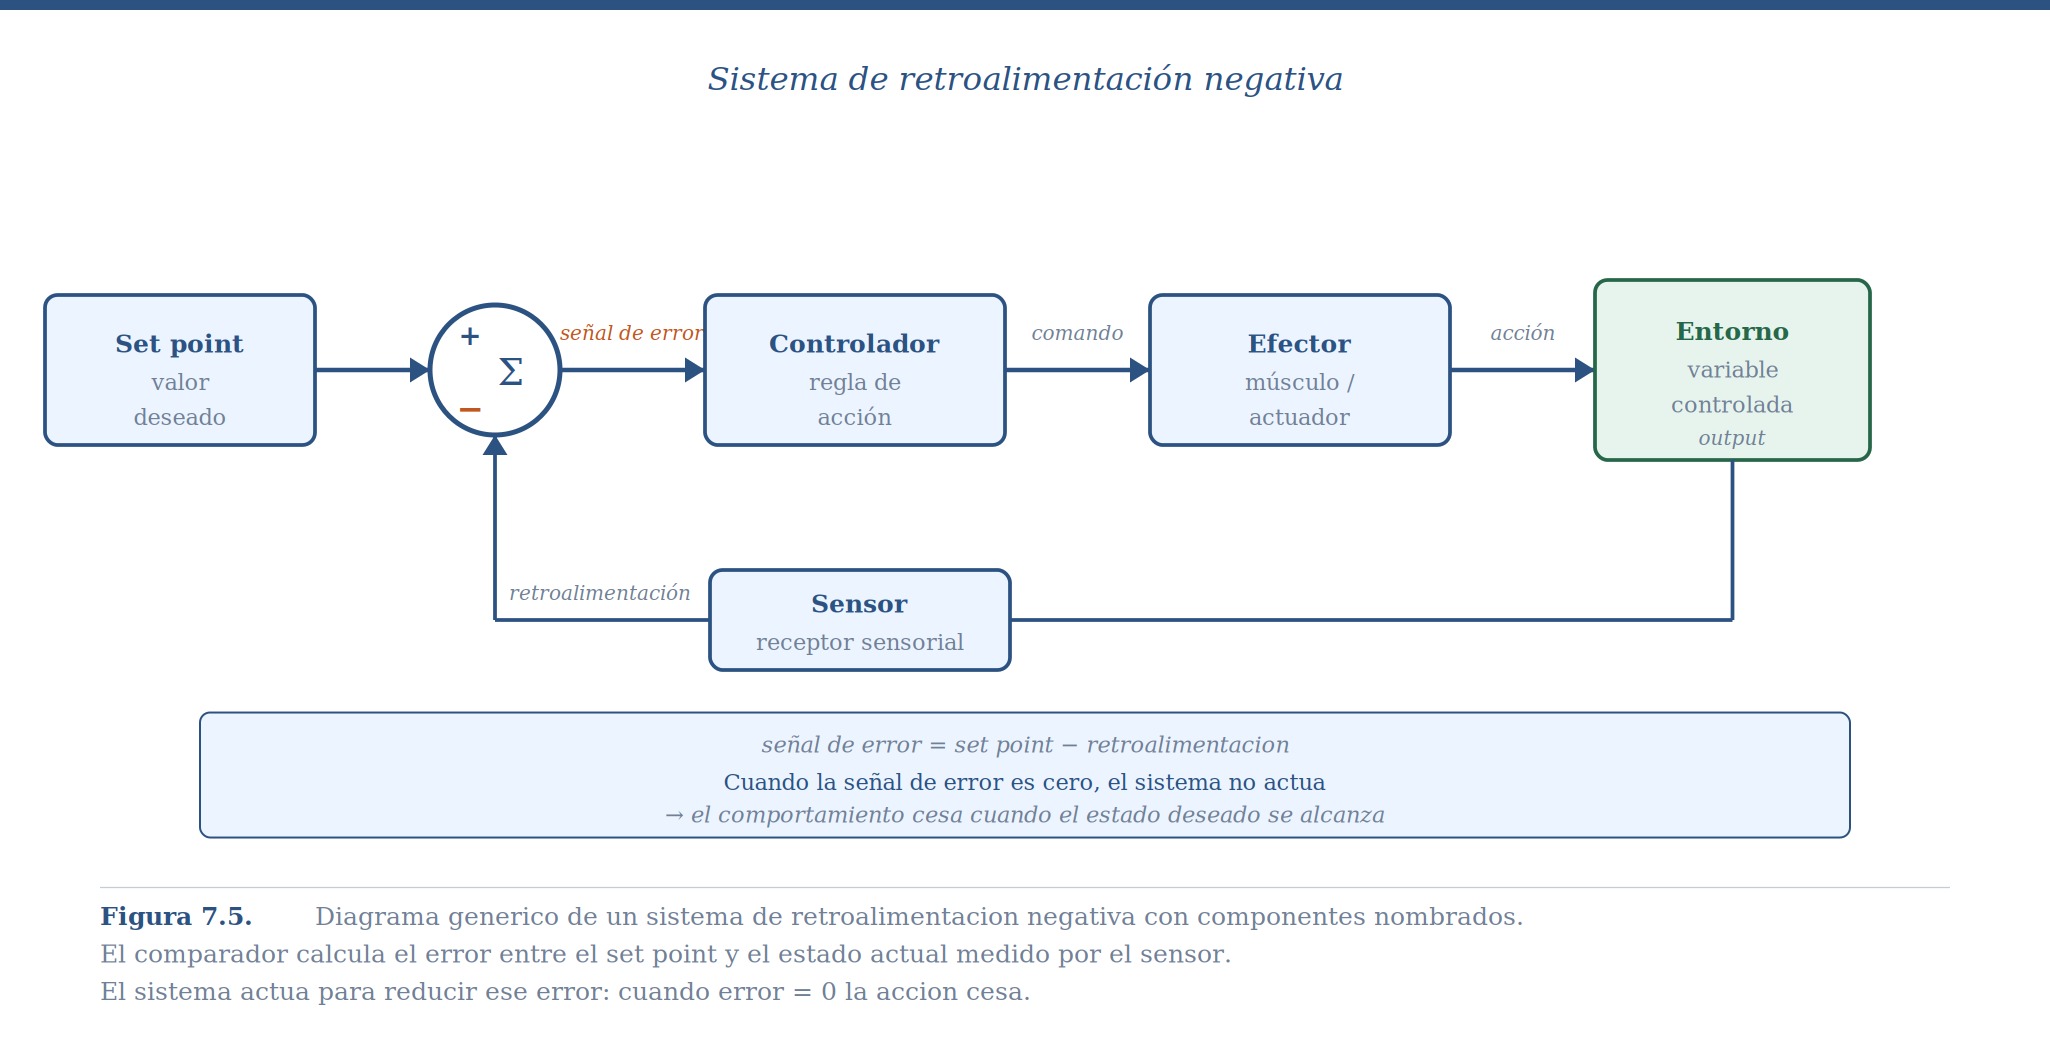
\includegraphics[keepaspectratio]{Figuras/fig7_5_retroalimentacion.png}}

}

\caption{Componentes del sistema de retroalimentación}

\end{figure}%

\begin{tcolorbox}[enhanced jigsaw, arc=.35mm, bottomrule=.15mm, breakable, colback=white, colframe=quarto-callout-note-color-frame, left=2mm, leftrule=.75mm, opacityback=0, rightrule=.15mm, toprule=.15mm]

\textbf{Descrioción}: Diagrama de retroalimentación con componentes
nombrados. Desired Output → Comparator → Error signal → Effectors
(calefactor/AC) → Output, con Sensor + Feedback signal completando el
lazo. El comparador integra la salida deseada con la señal de
retroalimentación del sensor para producir la señal de error.

\end{tcolorbox}

Esto contrasta con los \textbf{sistemas abiertos}, donde el
comportamiento responde al entorno pero no modifica la variable que lo
controla. Un calefactor encendido permanentemente sin importar la
temperatura es un sistema abierto. El golpe de lengua de una rana
capturando una mosca también: una vez iniciado, el movimiento se ejecuta
hasta completarse sin corrección durante su trayectoria. Y cubrir un ojo
en el experimento de tropotaxia transforma al organismo en un sistema
abierto: el giro nunca recibe señal de corrección, y el resultado es
rotación indefinida.

Vale la pena detenerse un momento para notar que, en este capítulo igual
que en el anterior, hemos aplicado sin nombrarlo el análisis de tres
niveles del Capítulo 1. El nivel computacional es orientarse hacia una
fuente de forma rápida y robusta. El nivel algorítmico es la comparación
simultánea bilateral, el cálculo de una señal de error, y la función de
control que transforma ese error en tasa de giro. El nivel de
implementación ---los circuitos neurales específicos, los
fotorreceptores, los músculos--- varía entre especies y no necesitamos
especificarlo para entender cómo funciona el sistema. Una polilla, un
robot de dos ruedas y un sistema de climatización doméstico comparten la
misma arquitectura algorítmica aunque sus implementaciones físicas no
tengan nada en común.

La \textbf{retroalimentación negativa} ocurre cuando el comportamiento
tiende a \emph{reducir} la señal de error ---la acción contrarresta la
desviación que la provocó. El nombre puede sonar paradójico, pero
refleja que la acción tiene signo opuesto al error. Es el caso de la
fototaxia y de toda regulación homeostática.

La \textbf{retroalimentación positiva} ocurre cuando el comportamiento
\emph{amplifica} la señal de error. La apertura de canales de sodio
durante un potencial de acción es el ejemplo canónico: la entrada de
iones positivos despolariza la membrana, lo que abre más canales, en una
cascada que solo se detiene cuando todos los canales están abiertos. Es
útil para producir transiciones rápidas y decisivas entre estados, pero
no puede servir como mecanismo de orientación.

\section{Las Cuatro Preguntas}\label{las-cuatro-preguntas}

Ante cualquier sistema de retroalimentación, conviene hacerse las mismas
cuatro preguntas en orden: ¿tiene el sistema un equilibrio? ¿Cuál es ese
equilibrio? ¿Cómo llega el sistema al equilibrio ---cuál es su dinámica?
¿Cómo responde ante una perturbación abrupta? Apliquémoslas al sistema
de fototaxia.

Para hacerlo concreto, necesitamos la función de control. Sea ω la tasa
de giro, S\_izq la estimulación del sensor izquierdo, y S\_der la del
derecho:

\[\omega = k \cdot (S_{der} - S_{izq})\]

La diferencia entre paréntesis es la señal de error: codifica tanto la
magnitud de la desviación como su dirección. Si S\_der \textgreater{}
S\_izq, la fuente está a la derecha, el error es positivo, y ω es
positivo (giro a la derecha). Si ambas son iguales, el error es cero y
el organismo sigue recto.

El parámetro \textbf{k} es la \emph{ganancia} del sistema: qué tan
importante es para el organismo una diferencia dada entre sus sensores.
Un k alto significa que diferencias pequeñas producen giros grandes; un
k bajo requiere diferencias grandes para producir giros apreciables.
Esta interpretación ---la ganancia como peso de una señal de
discrepancia--- reaparecerá en capítulos posteriores cuando veamos cómo
el aprendizaje modifica qué tanto le importa a un organismo la
diferencia entre lo que predijo y lo que ocurrió. En fototaxia negativa,
k \textless{} 0: ante más luz en el lado derecho, el organismo gira
hacia la \emph{izquierda}, alejándose. El signo de k define si el
sistema busca o evita la fuente.

\textbf{¿Tiene equilibrio?} Sí. El equilibrio ocurre cuando ω = 0, es
decir, cuando la señal de error es cero.

\textbf{¿Cuál es el equilibrio?} La señal de error es cero cuando S\_der
= S\_izq, lo que ocurre cuando el organismo apunta directamente hacia la
fuente (ángulo θ = 0°). Hay un segundo equilibrio matemático en θ =
180°, pero es inestable: cualquier perturbación mínima empuja al sistema
lejos de ese punto. El equilibrio adaptativo es el único estable.

\textbf{¿Cuál es la dinámica?} La señal de error es mayor cuando el
ángulo θ es grande y más pequeña cuando θ es pequeño. Esto significa que
el giro correctivo es grande cuando más lo necesitas y se va volviendo
cada vez más sutil conforme te acercas al equilibrio. La convergencia
que se desacelera al acercarse al equilibrio produce el patrón de
trayectoria observado en los experimentos: no una línea recta, sino una
\textbf{espiral que se cierra progresivamente} hacia la fuente. Cuanto
mayor el ángulo inicial, mayor la curvatura; cuanto más cercano al
equilibrio, más recta la trayectoria.

\begin{figure}

{\centering 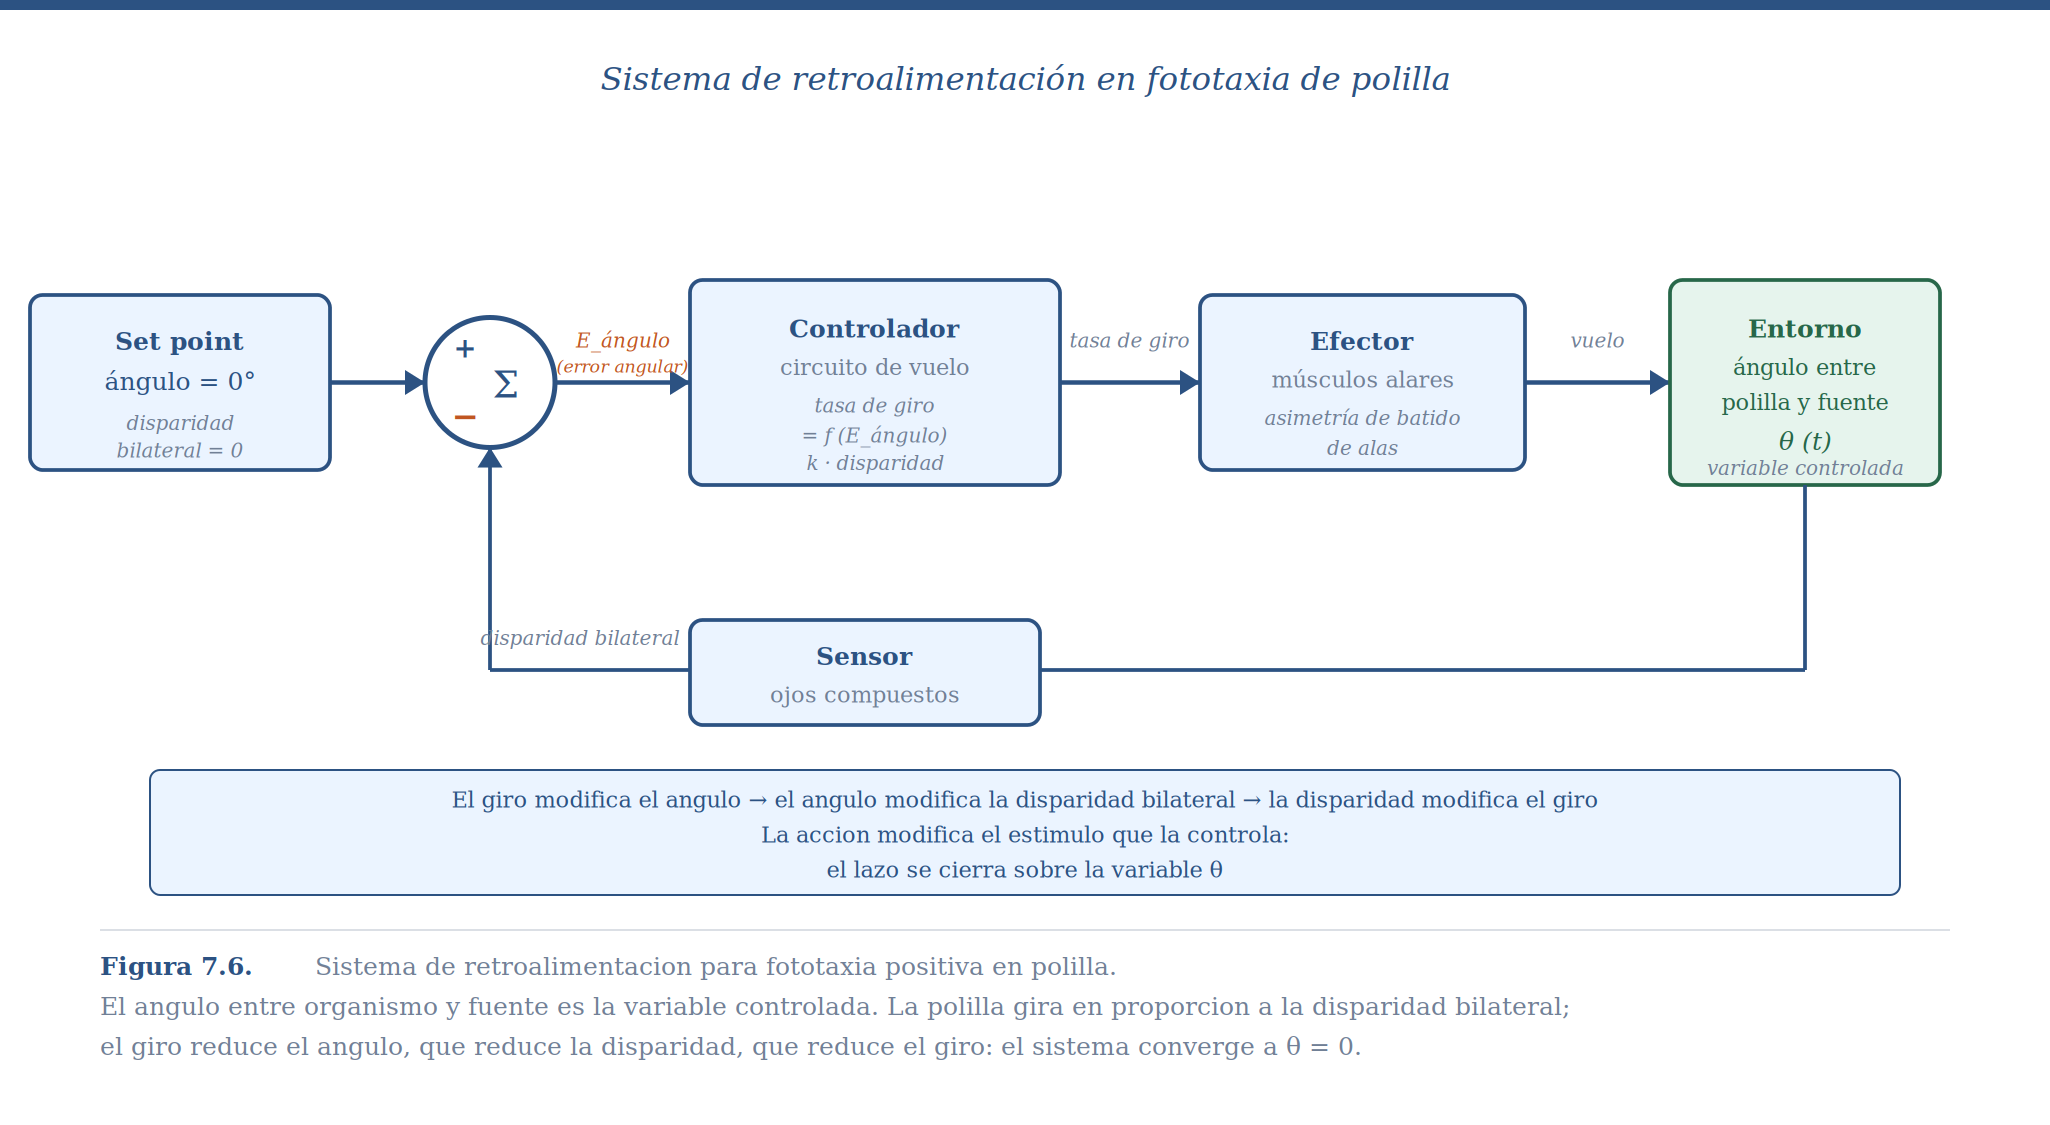
\includegraphics[width=7.8125in,height=\textheight,keepaspectratio]{Figuras/fig7_6_mariposa.png}

}

\caption{Sistema de retroalimentación de la mariposa}

\end{figure}%

\begin{tcolorbox}[enhanced jigsaw, arc=.35mm, bottomrule=.15mm, breakable, colback=white, colframe=quarto-callout-note-color-frame, left=2mm, leftrule=.75mm, opacityback=0, rightrule=.15mm, toprule=.15mm]

\textbf{Descripción}: Diagrama específico para la mariposa. Set point
(45°) → Comparador (E\_Angle) → Controller (Flying Decision-making
circuit) → Actor (Wing) → Flying, con Sensor (Compound eyes) + señal de
Angle cerrando el lazo. Los ángulos y nombres de señales corresponden a
las variables del sistema real.

La distinción entre \textbf{transitorio} y \textbf{estado estacionario}
es importante. El transitorio es el período de ajuste desde las
condiciones iniciales hasta el equilibrio ---la espiral de aproximación.
El estado estacionario es el comportamiento una vez alcanzado el
equilibrio. Cuando ocurre una perturbación (una ráfaga de viento que
desvía a la polilla), el sistema entra en un nuevo transitorio que lo
lleva de vuelta al estado estacionario.

\textbf{¿Cómo responde ante perturbación?} Una polilla con θ ≈ 0° recibe
una ráfaga de viento que la desvía a θ = 30°. Sin retroalimentación,
continuaría en esa dirección indefinidamente. Con retroalimentación: el
nuevo ángulo genera nueva disparidad, nueva señal de error, nuevo giro
correctivo, y la polilla vuelve al equilibrio. La perturbación es
compensada sin ninguna ``decisión'' explícita, simplemente por la
estructura del lazo. Una ventaja adicional: la robustez es independiente
del valor exacto de k. Tanto un organismo joven con músculos débiles
como uno adulto con músculos fuertes alcanzarán θ = 0°, solo que a
velocidades distintas.

\subsection{¿Qué tan buena es la función de
control?}\label{quuxe9-tan-buena-es-la-funciuxf3n-de-control}

La función de control que describimos ---girar a una tasa proporcional a
la disparidad bilateral--- funciona. La polilla llega a la fuente de
luz, el organismo con un ojo cubierto gira indefinidamente, el sistema
con demora oscila. Pero conviene preguntarse si esa función es la mejor
posible.

Considera dos organismos con la misma arquitectura sensorial pero
diferente ganancia \emph{k}. El primero tiene \emph{k} bajo: responde
débilmente a cada unidad de disparidad, tarda más en corregir una
desviación pero nunca sobrecompensa. El segundo tiene \emph{k} alto:
responde con fuerza a cada unidad de disparidad, corrige rápidamente
pero puede pasarse de largo. En un ambiente tranquilo, sin viento, con
la fuente de luz fija, el segundo organismo llega antes. En un ambiente
con perturbaciones frecuentes ---ráfagas de viento que desvían
continuamente al organismo de su trayectoria--- el organismo de \emph{k}
alto puede entrar en un ciclo de sobre-correcciones que lo hace menos
eficiente que el de \emph{k} bajo.

El valor óptimo de \emph{k} no existe en abstracto: existe en relación a
las características del entorno. En un entorno estable, alta ganancia es
mejor. En un entorno turbulento, ganancia moderada produce mejor
desempeño a largo plazo. La ``solución'' que vemos en cualquier especie
particular es el resultado de que la selección natural ajustó \emph{k}
al entorno promedio que esa especie ha enfrentado a lo largo de su
historia evolutiva. Una polilla que evolucionó en ambientes con poco
viento tiene, probablemente, una ganancia más alta que una especie
similar que evolucionó en zonas costeras con viento constante. No lo
hemos medido, pero la predicción es directa.

Esto revela algo importante sobre qué significa ``entender'' un
comportamiento. Si solo preguntamos cómo funciona el mecanismo ---nivel
algorítmico--- la respuesta es la función de control y el valor de
\emph{k} que tiene esa especie. Pero si preguntamos por qué ese valor
particular de \emph{k} ---por qué no más alto, por qué no más bajo--- la
respuesta requiere el nivel computacional: cuál es el problema
adaptativo que ese organismo resuelve y en qué tipo de entorno lo
resuelve. El valor de \emph{k} es la respuesta al problema; el problema
es lo que explica el valor de \emph{k}.

La misma lógica aplica a la forma de la función de control. La función
lineal ω = k·(S\_der − S\_izq) que usamos es la más simple posible.
Podría imaginarse una función que no solo usa la disparidad actual sino
la \emph{tasa de cambio} de la disparidad ---si la diferencia entre
sensores está creciendo rápidamente, corrige más agresivamente que si
está creciendo despacio, aunque en ambos casos el valor actual de la
disparidad sea el mismo. Esa función sería más eficiente ante blancos
móviles. Que organismos distintos tengan funciones de control distintas
es esperable: la función es la solución y el entorno define el problema.

Lo que hace óptima a la solución más sofisticada no es solo tener la
ganancia correcta, sino poder \emph{cambiar adaptativamente qué tan
importante es el error} dependiendo de la situación. Un organismo que en
entornos tranquilos usa \emph{k} alto para llegar rápido, y en entornos
turbulentos reduce automáticamente su ganancia para no oscilar ---ese
organismo supera a cualquier competidor con ganancia fija, sin importar
qué valor fijo tenga ese competidor. Esa capacidad de modificar la
importancia del error basándose en la experiencia reciente con el
entorno es, nuevamente, exactamente lo que los mecanismos de aprendizaje
permiten. La diferencia entre un sistema de retroalimentación con
\emph{k} fijo y un sistema que aprende el valor de \emph{k} adecuado no
es de tipo sino de escala temporal: el primero es la solución
filogenética al problema, el segundo es la solución ontogenética.

Cuando en el Bloque II veamos el parámetro α de los modelos de
aprendizaje, reconoceremos en él la misma pregunta que hemos planteado
aquí: ¿qué tan importante debería ser el error para este organismo, en
este entorno, en este momento?

\begin{quote}
\textbf{🕹️ ¡Prueba el Simulador Interactivo!}

Para explorar los conceptos de este capítulo en la práctica, abre el
siguiente simulador:

\href{https://colab.research.google.com/github/arbouria/Libro-ACA-2026/blob/main/Simuladores/retroalimentacion.ipynb}{\textbf{Abrir
Simulador sistemas de retroalimentación}}
\end{quote}

\textbf{Explora el primer simulador: fototaxias}

\textbf{Objetivo:} Descubrir cómo la ganancia k afecta la velocidad de
convergencia sin cambiar el equilibrio, y por qué cubrir un ojo
transforma el sistema de cerrado a abierto.

\emph{Básico:} Con θ₀ = 75° y k = 1.0, observa la trayectoria. ¿Es una
línea recta o una espiral? Antes de cambiar k, predice: si doblas k a
2.0, ¿el organismo llegará más rápido al mismo equilibrio, o llegará a
un equilibrio diferente?

\emph{Intermedio:} Activa la opción ``cubrir ojo izquierdo''. ¿Qué
ocurre con la trayectoria? ¿Puedes explicarlo en términos de la señal de
error?

\emph{Avanzado:} Cambia el signo de k (fototaxia negativa). ¿Hacia dónde
se mueve ahora el organismo? ¿Qué representa biológicamente este cambio
de signo?

\section{Regulación y
Servomecanismos}\label{regulaciuxf3n-y-servomecanismos}

Hasta aquí el set point ---el estado deseado--- ha sido fijo: ángulo
cero, fuente al frente. Hay una distinción útil entre dos tipos de
sistemas que aparecen con frecuencia.

En los sistemas de \textbf{regulación}, el set point es interno y
permanece relativamente fijo: la temperatura corporal de un mamífero
(\textasciitilde37°C), la concentración de glucosa en sangre, el pH de
los fluidos internos. El entorno cambia ---hace calor, hace frío, comes
mucho o poco--- pero el organismo corrige continuamente para mantener su
estado interno estable. Esto es lo que Cannon llamó homeostasis.

Los \textbf{servomecanismos} tienen un set point externo y variable: lo
que el sistema persigue cambia de posición en el tiempo. La fototaxia se
convierte en servomecanismo cuando la fuente de luz se mueve. Un misil
teledirigido es el ejemplo tecnológico ---no persigue un punto fijo,
sino un avión que se desplaza. El seguimiento ocular es el ejemplo
biológico cotidiano: cómo tus ojos rastrean un objeto en movimiento sin
que tengas que pensarlo.

La diferencia importa por sus limitaciones. Un sistema de regulación
puede fallar si la perturbación excede su capacidad correctiva. Un
servomecanismo puede fallar si el objetivo se mueve más rápido de lo que
el sistema puede seguir ---hay un límite de velocidad de seguimiento,
llamado ancho de banda, más allá del cual el sistema pierde el blanco.

\begin{quote}
\textbf{🕹️ ¡Sigue probando el Simulador Interactivo!}

\href{https://colab.research.google.com/github/arbouria/Libro-ACA-2026/blob/main/Simuladores/retroalimentacion.ipynb}{\textbf{Abrir
Simulador sistemas de retroalimentación}}
\end{quote}

\textbf{Explora el segundo simulador: Efecto de la Demora}

\emph{Básico:} Con k = 1.0 y sin demora, confirma la convergencia suave.
Añade una demora de 5 pasos. ¿Qué ocurre?

\emph{Avanzado:} Encuentra el valor de delay a partir del cual el
sistema comienza a oscilar para k = 1.0. Luego reduce k a la mitad. ¿El
mismo delay ahora produce oscilaciones o no? ¿Por qué la ganancia y la
demora interactúan?

\section{El Límite Fundamental: Esclavos del
Presente}\label{el-luxedmite-fundamental-esclavos-del-presente}

Los sistemas de retroalimentación son elegantes y poderosos, pero
comparten con el ascenso de colina una limitación que no puede
resolverse con más ganancia ni más sensores: son completamente
\textbf{reactivos}. Para que actúen, primero tiene que haber un error.
Siempre van un paso atrás.

El termostato no enciende antes de que la temperatura baje. Enciende
porque ya bajó. La polilla no gira antes de desviarse de la fuente. Gira
porque ya se desvió.

La regadera de agua caliente ilustra las consecuencias de esta
reactividad cuando hay demoras. Si hay un desfase significativo entre el
momento en que giras la perilla y el momento en que sientes el cambio de
temperatura, tiendes a sobrecompensar: ``¡demasiado fría!'' {[}giras
mucho hacia caliente{]} ``¡ahora demasiado caliente!'' {[}giras mucho
hacia fría{]} y así sucesivamente, oscilando alrededor de la temperatura
deseada sin llegar a ella. El problema no es la falta de
retroalimentación ---hay retroalimentación perfectamente funcional. El
problema es que la retroalimentación llega tarde: para cuando la señal
de corrección viaja de regreso, ya produjo un exceso en la dirección
contraria.

En entornos reales, las demoras son ubicuas. El sistema nervioso tarda
en procesar información sensorial. Los músculos tardan en responder. El
entorno tarda en cambiar en respuesta al comportamiento. Cada demora
puede desestabilizar un sistema de retroalimentación pura. La evolución
ha desarrollado estrategias para minimizar estas demoras, pero ninguna
las elimina por completo: la retroalimentación siempre reacciona después
del hecho.

\section{El Conductor y las
Gasolineras}\label{el-conductor-y-las-gasolineras}

Considera un problema cotidiano que lleva esta limitación a su punto más
claro.

Un conductor viaja por carretera y necesita recargar gasolina en algún
punto del trayecto. En principio podría resolver el problema con
retroalimentación pura: cuando el tanque llegue a cero, detenerse y
buscar gasolinera. El error dispara la respuesta. Problema: para cuando
el error se materializa, ya es demasiado tarde. En carretera abierta, el
tanque vacío puede dejarte varado entre gasolineras.

Una estrategia apenas mejor es fijar un umbral más alto: cargar cuando
quede un cuarto de tanque. Es retroalimentación mejorada, pero sigue
siendo reactiva: espera a que el estado del sistema alcance un nivel de
alerta antes de actuar. En una ciudad con gasolineras cada dos
kilómetros, esa estrategia funciona. En carretera del norte de México,
donde pueden pasar cien kilómetros entre gasolineras, puede no ser
suficiente.

La solución que adoptan los conductores experimentados es
cualitativamente diferente: aprenden la \emph{distribución espacial} de
las gasolineras en su ruta habitual. Saben que en tal tramo hay
gasolinera en el kilómetro 45, en el kilómetro 130, en el kilómetro 210.
Con ese conocimiento, el conductor carga gasolina no cuando el tanque
está bajo, sino \emph{antes de un tramo largo sin estaciones}. El
comportamiento ya no responde al estado actual del tanque; responde a
una predicción sobre necesidades futuras basada en conocimiento
aprendido del entorno.

La diferencia entre el conductor novato y el experimentado no es una
diferencia en el hardware ---ambos tienen los mismos instrumentos, el
mismo tanque, los mismos pies. La diferencia es que el conductor
experimentado aprendió relaciones en el mundo que le permiten predecir:
``si no cargo aquí, más adelante habrá problemas.'' Ese aprendizaje
---la adquisición de conocimiento sobre relaciones predictivas en el
entorno--- es precisamente lo que los sistemas de retroalimentación pura
no pueden hacer.

A este tipo de control se le llama \textbf{control anticipatorio} o
\emph{feedforward}. La distinción respecto a la retroalimentación es
precisa: en la retroalimentación, la señal que controla el
comportamiento es el error actual; en el feedforward, es una predicción
del error futuro derivada de un modelo aprendido del entorno. El
conductor experimentado opera en modo feedforward respecto a la
gasolina: carga antes de que aparezca el error, porque aprendió que
cierta señal presente predice una necesidad futura.

El feedforward no reemplaza a la retroalimentación ---la complementa. Si
una gasolinera esperada está cerrada, el conductor reactiva
inmediatamente la estrategia reactiva. Los sistemas biológicos más
robustos combinan ambos lazos: la retroalimentación garantiza la
corrección cuando algo sale mal; el feedforward evita que salga mal en
primer lugar.

\begin{quote}
\textbf{🕹️ ¡Sigue probando el Simulador Interactivo!}

\href{https://colab.research.google.com/github/arbouria/Libro-ACA-2026/blob/main/Simuladores/retroalimentacion.ipynb}{\textbf{Abrir
Simulador sistemas de retroalimentación}}
\end{quote}

\textbf{Explora el tercer simulador: Reactivo vs.~Anticipatorio}

\emph{Básico:} Con la distribución por defecto de gasolineras {[}40, 90,
250, 280, 450 km{]}, ¿cuál conductor llega al final de los 500 km? ¿En
qué kilómetro se queda varado el reactivo?

\emph{Avanzado:} Cambia las gasolineras a {[}20, 40, 60, 460, 480{]}
---muchas al inicio, casi ninguna al final. ¿Cambia el resultado? ¿Puede
el conductor reactivo tener éxito con algún umbral diferente al 15\%?
¿Cuál es el umbral mínimo que garantiza llegar?

\section{El Puente Hacia el
Aprendizaje}\label{el-puente-hacia-el-aprendizaje}

Este capítulo y el anterior han explorado mecanismos adaptativos que
funcionan sin aprendizaje: el ascenso de colina y la retroalimentación.
Ambos son herramientas poderosas para problemas relativamente estables y
locales. Ambos comparten la misma limitación: responden al mundo tal
como es \emph{ahora}, no al mundo tal como \emph{será}.

Para sobrevivir en un mundo donde eventos pasados predicen eventos
futuros, un organismo necesita algo más: poder modificar su
comportamiento basándose en experiencia acumulada. Aprender que cierto
estímulo predice cierta consecuencia, y ajustar la conducta \emph{antes}
de que la consecuencia llegue. En términos del conductor: aprender que
cierta señal en el entorno predice escasez de gasolineras adelante, y
actuar en consecuencia.

Esto es el condicionamiento asociativo, y es el tema central del resto
del libro. Los mecanismos que veremos ---condicionamiento pavloviano,
aprendizaje instrumental, modelos de reducción de error--- son todos
soluciones al mismo problema: ¿qué predice qué? ¿qué acción produce qué
consecuencia? Cuando un organismo resuelve ese problema, ya no vive
esclavizado al presente. Puede anticipar, prepararse, y actuar sobre el
futuro antes de que llegue.

\section{Comparación: Los Dos Mecanismos Sin
Historia}\label{comparaciuxf3n-los-dos-mecanismos-sin-historia}

{\def\LTcaptype{none} % do not increment counter
\begin{longtable}[]{@{}
  >{\raggedright\arraybackslash}p{(\linewidth - 4\tabcolsep) * \real{0.3333}}
  >{\raggedright\arraybackslash}p{(\linewidth - 4\tabcolsep) * \real{0.3333}}
  >{\raggedright\arraybackslash}p{(\linewidth - 4\tabcolsep) * \real{0.3333}}@{}}
\toprule\noalign{}
\begin{minipage}[b]{\linewidth}\raggedright
\end{minipage} & \begin{minipage}[b]{\linewidth}\raggedright
Ascenso de Colina (Cap. 4)
\end{minipage} & \begin{minipage}[b]{\linewidth}\raggedright
Retroalimentación (Cap. 5)
\end{minipage} \\
\midrule\noalign{}
\endhead
\bottomrule\noalign{}
\endlastfoot
Tipo de comparación & Sucesiva (ahora vs.~antes) & Simultánea (derecha
vs.~izquierda) \\
Sensores requeridos & Uno solo & Bilaterales (dos) \\
Información direccional & No ---solo tendencia local & Sí ---dirección
inmediata \\
Velocidad de convergencia & Lenta, sinuosa & Rápida, en espiral \\
Requiere memoria & Sí (valor previo) & No (comparación instantánea) \\
Robustez ante perturbaciones & Moderada & Alta \\
\end{longtable}
}

Ambos mecanismos son adaptativos y complementarios. Muchos organismos
los usan en diferentes contextos o en combinación. Lo que comparten ---y
lo que justifica estudiarlos juntos--- es la limitación que abre la
puerta al aprendizaje: son reactivos. No tienen historia, no tienen
predicción, no tienen modelo del futuro.

\section{Ejercicios de
Comprensión}\label{ejercicios-de-comprensiuxf3n-2}

\textbf{1.} Para cada comportamiento, decide si es (a) ascenso de
colina, (b) taxia, (c) retroalimentación con set point interno, o (d)
sistema abierto sin retroalimentación: un murciélago ajusta la dirección
de vuelo basándose en diferencias de tiempo entre la llegada del eco a
cada oído; una planta cierra sus hojas al detectar vibración; un humano
mantiene su temperatura corporal en 37°C; un caracol navega hacia mayor
humedad comparando su situación actual con la de hace un minuto.

\textbf{2.} Dibuja el diagrama de lazo de retroalimentación para la
termorregulación en un mamífero. Identifica el sensor, el comparador, el
controlador, el efector, y la función de retroalimentación. ¿Cuál es el
set point? ¿Cuál es la señal de error cuando la temperatura ambiente
baja bruscamente?

\textbf{3.} La función de control de una polilla es ω = k·(S\_der −
S\_izq) con k = 2. En un momento dado, S\_der = 8 y S\_izq = 5. ¿Cuál es
la tasa de giro? ¿En qué dirección está la fuente? ¿Qué ocurre en el
siguiente instante si el giro fue efectivo y ahora S\_der = 6.5 y S\_izq
= 6.5?

\textbf{4.} El experimento de cubrir un ojo transforma al organismo de
un sistema cerrado a uno abierto. Explica por qué en términos de las dos
ecuaciones del sistema (función de control y función de
retroalimentación). ¿Cuál de las dos ecuaciones deja de funcionar
correctamente?

\textbf{5.} Diseña el sistema de retroalimentación para un robot que
debe seguir una línea negra en el piso usando dos sensores de luz en la
parte frontal inferior. Especifica: (a) cuál es la señal de error, (b)
cómo varía el signo de k según si el robot va hacia la línea o se aleja,
(c) qué ocurre cuando el robot cruza la línea completamente y ambos
sensores ven blanco.

\textbf{6.} El ejemplo del conductor y las gasolineras ilustra la
diferencia entre reactivo y anticipatorio. Piensa en un ejemplo de tu
propia vida donde aplicas una estrategia anticipatoria. ¿Qué señal usas
como predictor? ¿Cuándo y cómo aprendiste que esa señal predice la
necesidad futura? ¿Recuerdas haber fallado ---usando la estrategia
reactiva--- antes de aprender la anticipatoria?

\section{Para Profundizar}\label{para-profundizar}

\textbf{Fraenkel, G. S., \& Gunn, D. L. (1961).} \emph{The Orientation
of Animals: Kineses, Taxes and Compass Reactions.} Dover. El tratado
clásico. Los capítulos 2--4 cubren la evidencia experimental en taxias
con más detalle del que fue posible aquí.

\textbf{Braitenberg, V. (1984).} \emph{Vehicles: Experiments in
Synthetic Psychology.} MIT Press. Una joya conceptual: comportamientos
sorprendentemente complejos emergen de sistemas de retroalimentación
simple. Breve y completamente accesible.

\textbf{Powers, W. T. (1973).} \emph{Behavior: The Control of
Perception.} Aldine. Un argumento radical: todo comportamiento animal
es, fundamentalmente, control de percepción mediante retroalimentación.
Controversial pero influyente.

\textbf{Ashby, W. R. (1956).} \emph{An Introduction to Cybernetics.}
Chapman \& Hall. Los fundamentos matemáticos de los sistemas de
retroalimentación, escritos con claridad excepcional. Los capítulos 1--3
son suficientes para los propósitos de este curso.

\bookmarksetup{startatroot}

\chapter{El Problema de la Asignación de
Crédito}\label{el-problema-de-la-asignaciuxf3n-de-cruxe9dito-1}

Al final del capítulo anterior dejamos a nuestro organismo en una
situación paradójica. Los sistemas de retroalimentación que describimos
son notablemente eficaces: pueden orientar un cuerpo hacia una fuente de
luz, mantener la temperatura dentro de un margen preciso, seguir una
presa en movimiento. Pero tienen una limitación que el ejemplo del
conductor y las gasolineras ilustró de manera directa: responden a lo
que está ocurriendo ahora, sin ninguna capacidad de anticipar lo que
está por ocurrir. El conductor que carga gasolina solo cuando el tanque
ya está vacío llegará varado tarde o temprano. El conductor
experimentado actúa antes ---carga cuando ve que se aproxima un tramo
largo, porque ha aprendido que esa señal predice la necesidad futura.

Ese salto, de reactivo a anticipatorio, requiere algo que los mecanismos
del Bloque I no tenían: la capacidad de aprender que ciertos eventos del
entorno predicen la llegada de sucesos biológicamente importantes. Pero
esto introduce de inmediato un problema que no es trivial. Cuando ocurre
algo importante ---aparece comida, ataca un depredador, se produce un
malestar--- el entorno está lleno de estímulos simultáneos y el pasado
está lleno de eventos candidatos. ¿A cuál de todos ellos se le debe
atribuir la responsabilidad? ¿Qué evento, de entre los centenares que
precedieron al suceso, fue realmente su causa?

A este problema de adaptación se le conoce como el \textbf{problema de
la asignación de crédito}, y es el tema central de este capítulo.

\section{El Problema: Un Espacio Enorme de
Candidatos}\label{el-problema-un-espacio-enorme-de-candidatos}

Considera la situación concreta de un perro callejero que encuentra
comida en una banqueta. En ese momento hay docenas de estímulos
presentes simultáneamente: el olor del asfalto húmedo, el sonido de una
bocina lejana, la figura de un transeúnte que se aleja, el color de la
bolsa que contenía la comida, la hora del día, el olor particular del
barrio. Y más allá de los estímulos presentes, hay una historia de
eventos que ocurrieron antes: algo cruzó por ahí cinco minutos atrás,
hubo un camión de basura en la mañana, llovió ayer. Cualquiera de estos
factores podría, en principio, predecir dónde y cuándo aparecerá comida
en el futuro.

O considera tu propia experiencia: regresas a casa después de comer en
un restaurante nuevo y experimentas un fuerte malestar estomacal. ¿Qué
lo causó? Las posibilidades son abrumadoras. Podría ser el platillo que
ordenaste, el olor del restaurante, la música que sonaba, algo que
comiste ayer, algo que tocaste en el transporte público, el estrés
acumulado del día. Esta lista podría extenderse indefinidamente hacia el
pasado. Sin algún mecanismo que filtre ese espacio de posibilidades, el
aprendizaje sería computacionalmente intratable ---un organismo que
evaluara sistemáticamente cada candidato posible quedaría paralizado
antes de poder actuar.

Y sin embargo, la mayoría de los organismos aprenden relaciones
predictivas con una eficiencia sorprendente, en tiempo real, sin acceso
a bases de datos ni laboratorio de estadística. La pregunta es cómo.

La respuesta es que los organismos no buscan en todo el espacio de
candidatos. Buscan en un subconjunto reducido y ordenado, definido por
un conjunto de reglas que llamamos \textbf{sesgos inductivos}. Estos
sesgos hacen dos cosas: primero, reducen drásticamente el espacio de
candidatos posibles; segundo, establecen un orden de prioridad para
evaluarlos. Antes de examinarlos en detalle, conviene preguntarse de
dónde vienen y por qué tienen la forma que tienen.

\section{El Genoma Como Archivo
Causal}\label{el-genoma-como-archivo-causal}

El genoma no es un acumulador indiferente de variación aleatoria. La
fracción del genoma que ha sido modelada por la selección natural ---la
parte que afecta el éxito reproductivo y que ha cambiado bajo la presión
del entorno--- es, en sentido literal, un registro comprimido de las
regularidades estadísticas del entorno ancestral: qué eventos tendían a
co-ocurrir, con qué frecuencias, en qué secuencias temporales. Cada
generación, los organismos con mecanismos mejor calibrados a esas
regularidades dejaron más descendientes, y ese proceso iterativo ---que
la ecuación de Price formalizó en el capítulo sobre selección natural---
produjo, acumulativamente, un sistema nervioso que llega al mundo ya
``informado'' sobre la estructura causal más probable de su entorno.

Desde esta perspectiva, la selección natural es una forma de aprendizaje
filogenético. No es el aprendizaje de un organismo individual durante su
vida, sino el aprendizaje de una especie a lo largo de sus generaciones.
Y al igual que el aprendizaje individual produce cambios en el organismo
que reflejan las regularidades del entorno que ese individuo ha
experimentado, el aprendizaje filogenético produce cambios en el acervo
genético que reflejan las regularidades del entorno que esa especie ha
habitado. Los sesgos inductivos son el producto más visible de ese
proceso: no restricciones arbitrarias impuestas desde fuera, sino
conocimiento filogenético sobre la estructura causal del mundo,
destilado por selección durante escalas de tiempo inaccesibles para
cualquier individuo.

Veremos más adelante en el curso que hay una manera precisa de medir
cuánta información contiene un organismo sobre su entorno, y que la
selección natural puede entenderse como el proceso que maximiza esa
cantidad, generación tras generación. Por ahora, lo que importa es la
consecuencia directa para los sesgos: si el entorno ancestral tenía una
estructura causal particular ---si los eventos biológicamente
importantes tendían a ser precedidos por ciertas clases de estímulos,
con ciertas demoras temporales, en ciertos contextos sensoriales---
entonces la selección favorecerá organismos que busquen primero en esa
parte del espacio de candidatos. Eso es exactamente lo que observaremos.

\section{El Sistema de Comportamiento Como Primer
Filtro}\label{el-sistema-de-comportamiento-como-primer-filtro}

Antes de examinar los sesgos inductivos específicos, hay un nivel de
organización más fundamental que los estructura a todos: los
\textbf{sistemas de comportamiento}.

Jerry Hogan y John Timberlake desarrollaron una perspectiva que ha sido
influyente precisamente porque da sustrato funcional a la idea de
relevancia biológica. Su propuesta es que el comportamiento de los
organismos no es una colección arbitraria de respuestas inconexas, sino
que está organizado en sistemas funcionales pre-estructurados por la
evolución. Un sistema de comportamiento es un conjunto coordinado de
mecanismos perceptuales, motivacionales y motores que evolucionó para
resolver un problema adaptativo específico: el sistema de alimentación,
el sistema de defensa ante depredadores, el sistema reproductivo. Cada
uno tiene sus propias estructuras de detección, sus propias respuestas
características, su propia lógica temporal.

Lo que hace crucial esta organización para la asignación de crédito es
la siguiente observación: cuando ocurre un suceso biológicamente
importante, no genera una activación genérica del organismo. Activa el
sistema de comportamiento apropiado para ese tipo de suceso. La
presentación de comida activa el sistema de alimentación, con todas sus
estructuras perceptuales y motoras. Un depredador activa el sistema de
defensa. Y esta activación de un sistema específico tiene una
consecuencia inmediata: reduce drásticamente el espacio de estímulos que
serán siquiera considerados como candidatos a la asignación de crédito.

Cuando el sistema de alimentación está activo, los estímulos relevantes
para la alimentación ---sabores, olores, señales visuales de comida---
son procesados preferentemente. Los estímulos irrelevantes para la
alimentación ---sonidos ambientales neutros, características del
suelo--- reciben mucha menos atención. El sistema de comportamiento
funciona así como un filtro atencional de primer orden: antes de que
operen los sesgos específicos que examinaremos a continuación, el tipo
de suceso biológicamente importante ya ha limitado severamente el
espacio de búsqueda.

En el lenguaje del aprendizaje automático contemporáneo, podríamos decir
que los sistemas de comportamiento son \emph{priors} estructurados: no
comenzamos asignando probabilidades iguales a todos los estímulos del
universo, sino con un espacio de hipótesis ya preconfigurado donde
ciertas dimensiones de estimulación son a priori más probables de ser
relevantes, dado el tipo de suceso que ocurrió. Este insight de Hogan y
Timberlake no es solo teórico ---lo veremos confirmado empíricamente en
cada uno de los experimentos que siguen.

\section{El Primer Sesgo: Contigüidad
Temporal}\label{el-primer-sesgo-contiguxfcidad-temporal}

\subsection{El Experimento de Pavlov}\label{el-experimento-de-pavlov}

Dentro del sistema de comportamiento que el suceso biológicamente
importante ha activado, el primer sesgo que opera es la
\textbf{contigüidad temporal}: los eventos que ocurrieron
aproximadamente al mismo tiempo que el suceso son candidatos más
plausibles que los que ocurrieron hace mucho tiempo. La intuición es
directa ---la mayoría de los mecanismos causales biológicamente
relevantes producen sus efectos con relativa rapidez--- y fue el primero
en recibir atención sistemática.

A principios del siglo XX, Ivan Pavlov le dio sentido experimental a
este sesgo. El protocolo básico es conocido: a un perro se le presenta
un estímulo auditivo ---un tono--- seguido por acceso a comida. El tono,
inicialmente neutral, adquiere la capacidad de provocar salivación
precisamente porque predice la llegada de la comida. Pavlov y sus
sucesores exploraron sistemáticamente distintas variaciones temporales
del procedimiento. En el condicionamiento de demora, el tono inicia
primero y la comida llega mientras el tono sigue activo: el intervalo
relevante es el que transcurre entre el inicio del tono y el inicio de
la comida. Cuando ese intervalo es corto ---de medio segundo a dos
segundos--- el aprendizaje es excelente; cuando se extiende a varios
segundos o minutos, el aprendizaje disminuye sistemáticamente aunque el
tono permanezca presente. En el condicionamiento de huella, el tono
termina completamente antes de que inicie la comida, dejando un
intervalo vacío entre ambos; el aprendizaje decrece con la duración de
ese intervalo. Y en el condicionamiento hacia atrás ---la comida se
presenta primero, el tono después--- el aprendizaje es mínimo o nulo.

\begin{figure}[H]

\centering{

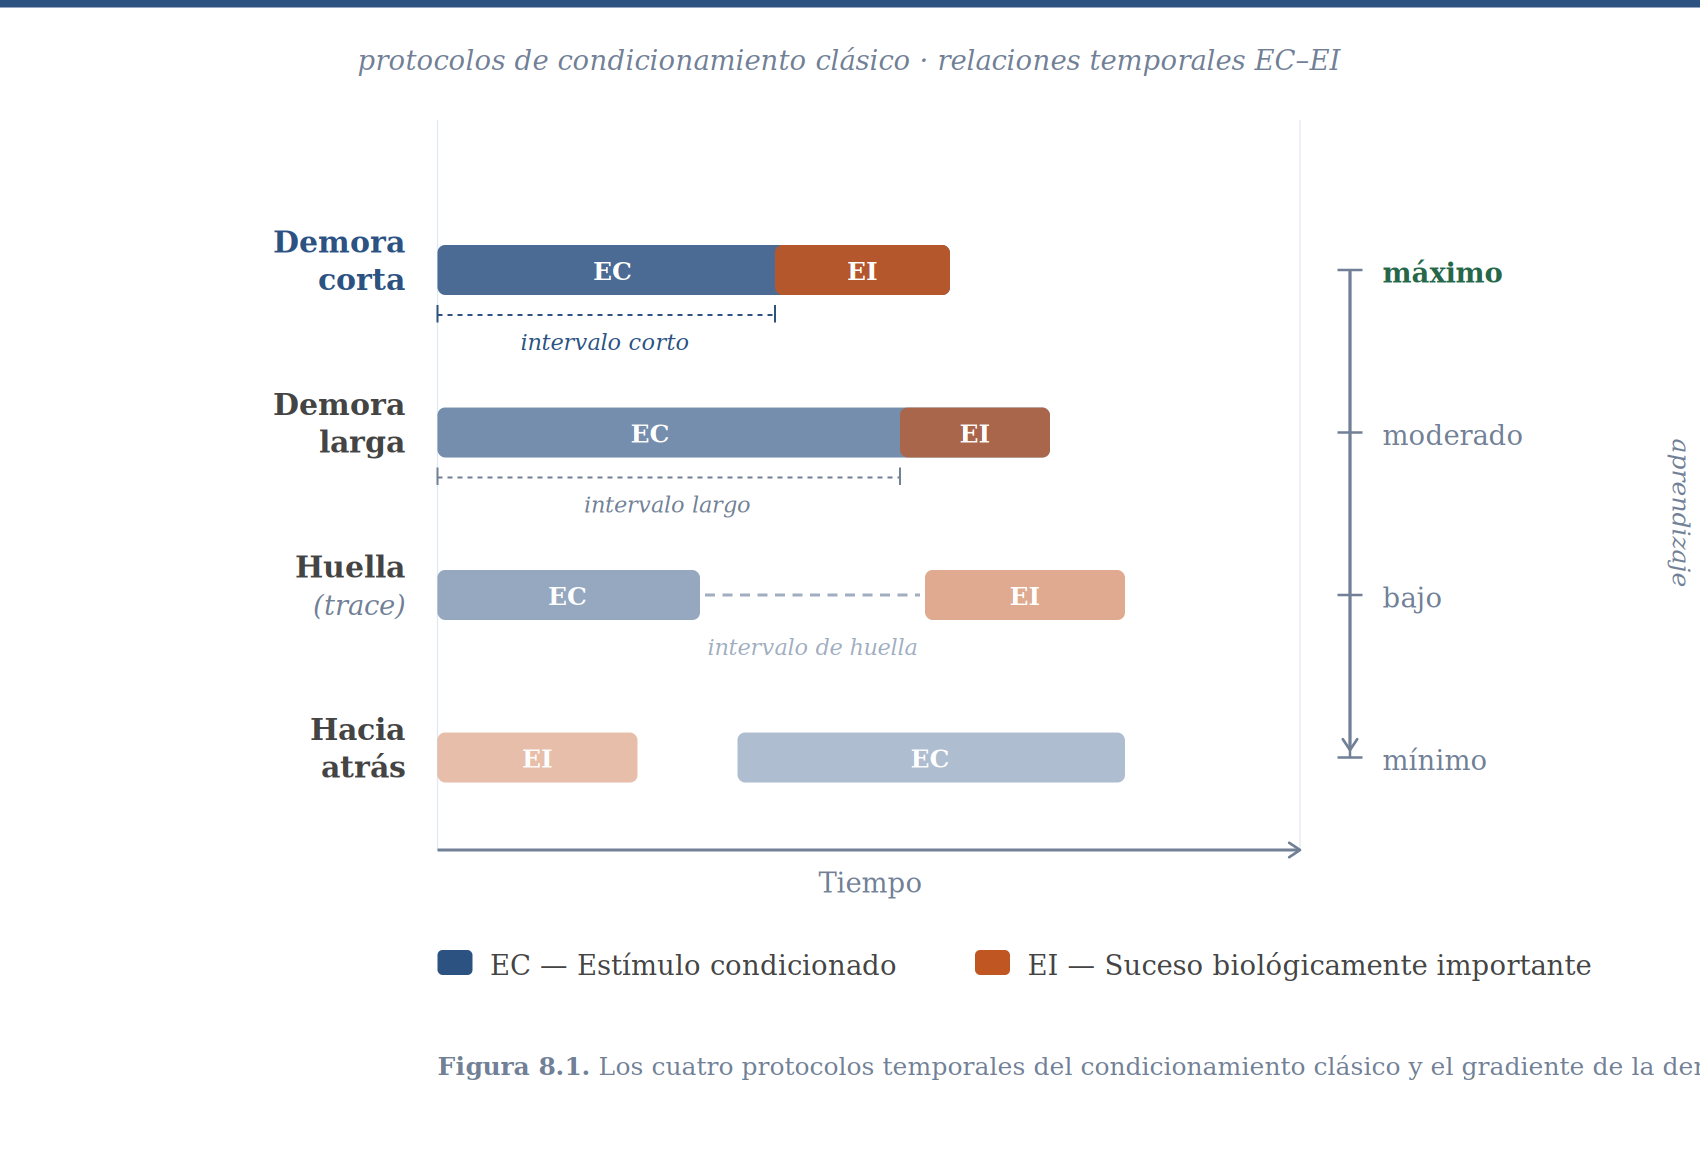
\includegraphics[width=0.9\linewidth,height=\textheight,keepaspectratio]{Figuras/fig8_1_protocolos_temporales.png}

}

\caption{\label{fig-protocolos_temporales}Protocolos temporales del
condicionamiento clásico y gradiente de la demora.}

\end{figure}%

\begin{quote}
\textbf{Note}

\textbf{Descripción.} Los cuatro procedimientos temporales básicos del
condicionamiento clásico. Eje horizontal: tiempo. Las barras sólidas
indican la duración de cada estímulo. De arriba a abajo:
condicionamiento de demora corta (EC activo cuando llega el EI ---
máximo aprendizaje), demora larga (EC aún activo pero intervalo mayor),
huella (EC apagado antes de que llegue el EI --- intervalo de huella
vacío), y condicionamiento hacia atrás (EI antes que EC --- mínimo
aprendizaje). La flecha lateral indica el gradiente de la demora: la
fuerza del condicionamiento disminuye sistemáticamente conforme aumenta
el intervalo entre el inicio del EC y el inicio del EI.
\end{quote}

El patrón que emerge de estos estudios es el \textbf{gradiente de la
demora}: la fuerza del condicionamiento disminuye sistemáticamente
conforme aumenta el tiempo entre el estímulo candidato y el suceso
biológicamente importante. Dependiendo de la preparación, después de
menos de un minuto de intervalo frecuentemente no se observa aprendizaje
alguno. Nota que este gradiente no es binario ---contiguo o no
contiguo--- sino continuo: mientras más cercanos en el tiempo, mayor es
el crédito asignado.

El gradiente de la demora tiene una interpretación directa en términos
del problema de asignación de crédito. Frente al espacio enorme de
candidatos posibles, el organismo descarta todos los que no ocurrieron
aproximadamente al mismo tiempo que el suceso. El espacio se reduce
radicalmente. Pero conviene preguntarse de inmediato: ¿es siempre esto
una buena política?

\section{¿Es la Contigüidad Condición Necesaria? El Experimento de
García}\label{es-la-contiguxfcidad-condiciuxf3n-necesaria-el-experimento-de-garcuxeda}

El gradiente de la demora parecía establecer la contigüidad como un
principio fundamental: sin proximidad temporal, no hay aprendizaje. Pero
esta generalización ya había empezado a ceder antes de que alguien la
pusiera explícitamente a prueba.

A finales de los años cincuenta, John García trabajaba en un laboratorio
de radiación estudiando los efectos de la exposición sobre ratas.
Observó algo que nadie buscaba: las ratas desarrollaban aversión a su
comida habitual después de ser irradiadas, aunque el malestar gástrico
causado por la radiación tardara horas en aparecer. Nadie había diseñado
ese experimento. Las horas de demora entre la ingesta y el malestar
deberían haber hecho el aprendizaje imposible, según el gradiente que
Pavlov había establecido. Y sin embargo ocurría.

García diseñó entonces un experimento para explorar ese resultado de
manera sistemática. El diseño publicado con Koelling en 1966 tiene una
elegancia particular: en lugar de manipular una variable a la vez, pone
en juego dos tipos de estímulos y dos tipos de consecuencia
simultáneamente, de modo que los resultados de los cuatro grupos se
iluminan mutuamente.

A todas las ratas se les daba acceso a un bebedero con agua azucarada;
cada lametazo producía simultáneamente un tono y un destello de luz.
Así, el estímulo era siempre un compuesto: sabor por un lado, señal
audiovisual por otro. Luego los grupos se separaban. A la mitad se les
administraba una descarga eléctrica inmediata con cada lametazo; a la
otra mitad se les inyectaba una sustancia que producía malestar
gastrointestinal con un retraso de horas.

\begin{figure}[H]

\centering{

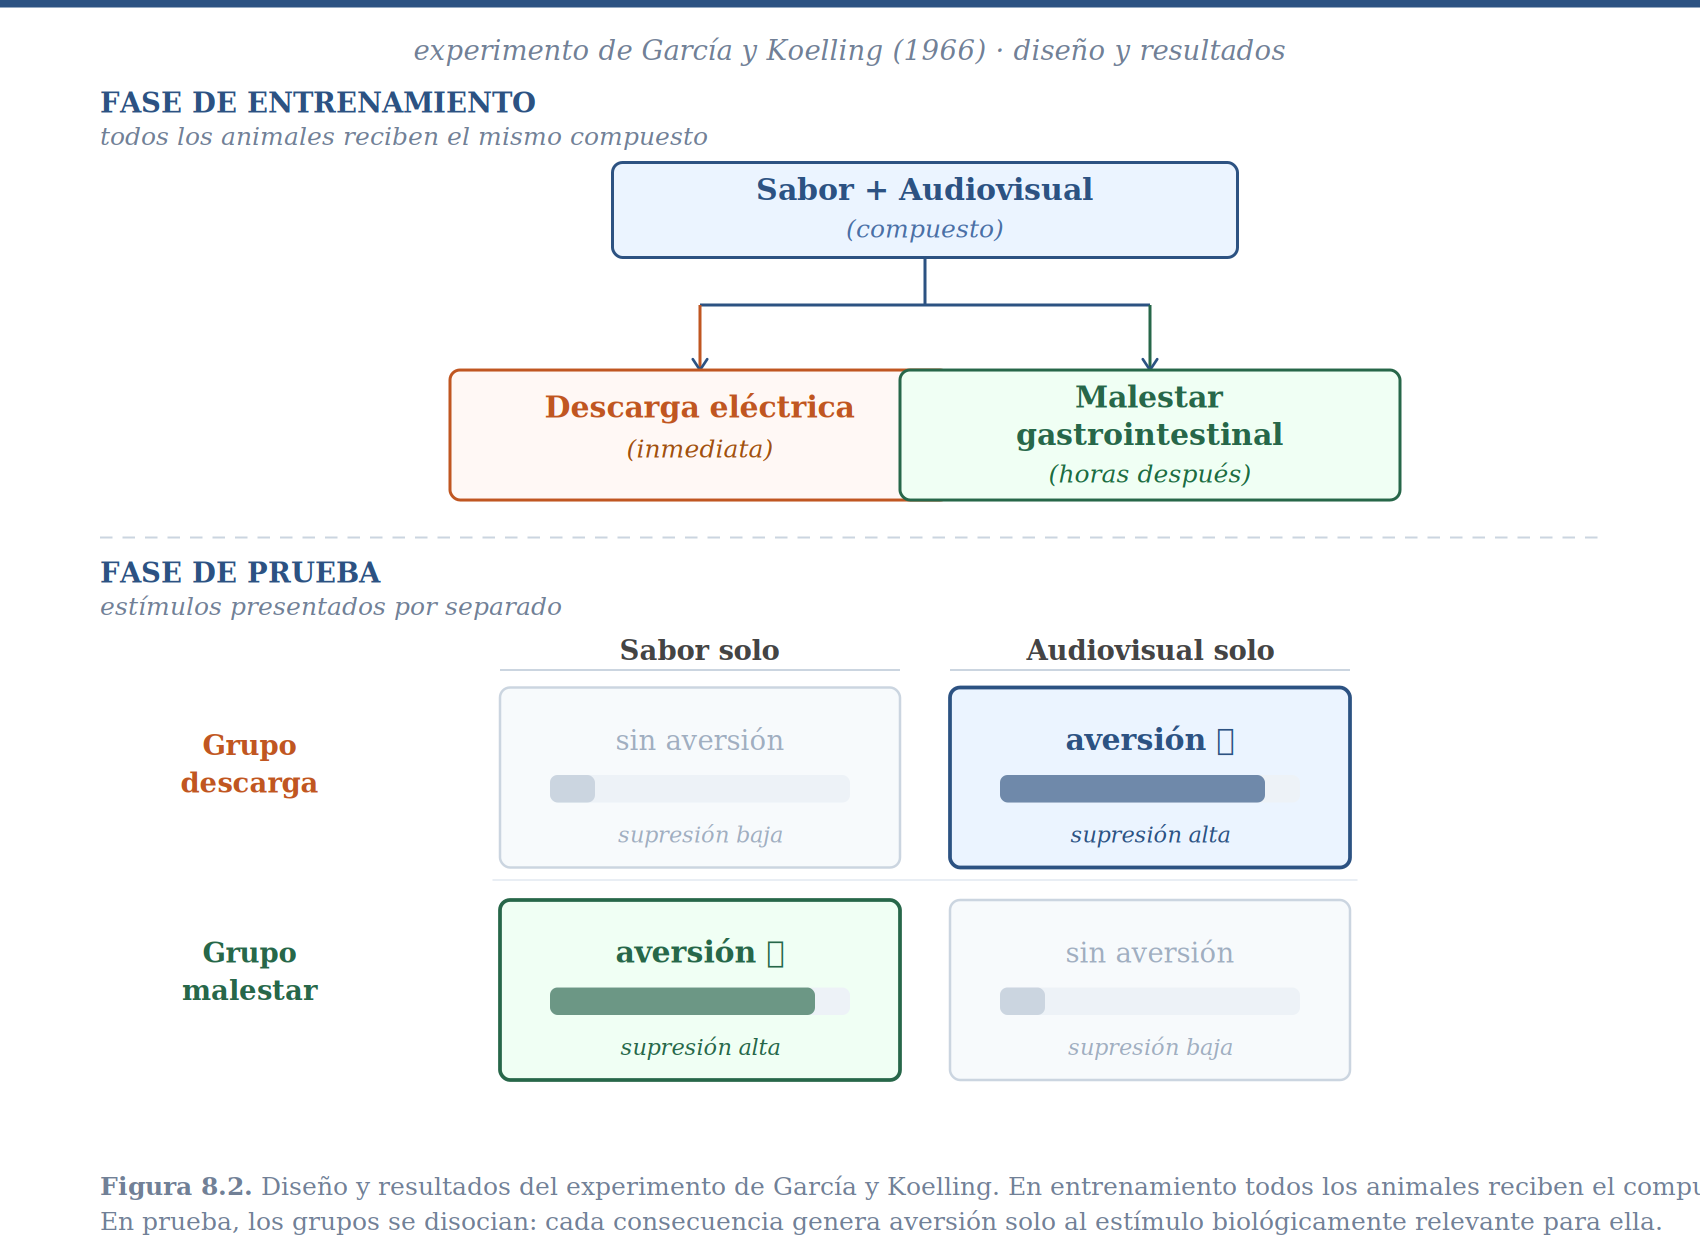
\includegraphics[width=0.9\linewidth,height=\textheight,keepaspectratio]{Figuras/fig8_2_garcia_koelling.png}

}

\caption{\label{fig-garcia}Diseño y resultados del experimento de García
y Koelling (1966).}

\end{figure}%

\begin{quote}
\textbf{Note}

\textbf{Descripción.} En la fase de entrenamiento todos los animales
reciben el compuesto sabor+audiovisual contiguo con su respectiva
consecuencia: descarga eléctrica inmediata (grupo izquierdo) o malestar
gastrointestinal con retraso de horas (grupo derecho). En la fase de
prueba los estímulos se presentan por separado. El grupo con descarga
desarrolla aversión al estímulo audiovisual pero no al sabor; el grupo
con malestar desarrolla aversión al sabor pero no al audiovisual. El
mismo compuesto produce resultados completamente distintos dependiendo
del tipo de consecuencia, lo que demuestra que la naturaleza del suceso
biológicamente importante determina qué dimensiones del estímulo entran
en el espacio de candidatos para la asignación de crédito.
\end{quote}

Los resultados cruzaron de manera llamativa. Las ratas con descarga
eléctrica no dejaron de beber el agua dulce, pero sí evitaban el
bebedero cuando este producía el tono y la luz. Las ratas con malestar
gastrointestinal hacían exactamente lo contrario: dejaban de beber el
agua dulce, pero no presentaban aversión al tono ni a la luz.

Los dos grupos no ilustran el mismo fenómeno y vale la pena separarlos.

En el grupo de descarga, ambos componentes del compuesto eran igualmente
contiguos con la consecuencia ---el shock llegaba con cada lametazo, sin
demora. A pesar de esa igualdad temporal, el aprendizaje fue selectivo:
solo el estímulo audiovisual adquirió valor aversivo. Este es el
resultado más limpio del experimento. Con contigüidad idéntica para los
dos componentes, el sistema de defensa seleccionó uno y descartó el
otro. La contigüidad no decidió qué se aprendió: la naturaleza del
suceso biológicamente importante sí lo hizo.

En el grupo de enfermedad, el resultado es diferente en su estructura
aunque paralelo en su forma: las ratas aprendieron a evitar el sabor, no
el audiovisual. Pero la consecuencia llegó horas después ---territorio
completamente fuera del gradiente pavloviano. El aprendizaje ocurrió de
todas maneras. La contigüidad no era condición necesaria. La explicación
no está en el mecanismo sino en la función: para un omnívoro que puede
ingerir toxinas naturales cuyo efecto tarda horas en manifestarse, un
sistema de aprendizaje que requiriera contigüidad estricta entre sabor y
malestar sería inútil. La selección natural produjo, en cambio, un
sistema preparado para asociar sabores con consecuencias
gastrointestinales a través de demoras que reflejan la firma temporal
real de los venenos en el entorno ancestral.

Que la contigüidad no sea condición necesaria no significa que sea
irrelevante. Estudios posteriores que variaron la demora entre la
ingesta y el malestar encontraron un gradiente: la aversión aprendida
era más intensa cuando el intervalo era más corto. Y cuando se
presentaban dos sabores antes de inducir el malestar, la aversión se
formaba con mayor fuerza hacia el sabor temporalmente más cercano a la
consecuencia. El sistema de aprendizaje sigue siendo sensible a la
proximidad temporal ---pero la ventana dentro de la cual esa
sensibilidad opera es mucho más ancha que la que Pavlov había descrito,
y esa anchura es en sí misma una adaptación evolutiva.

A lo que acabamos de describir ---la dependencia del tipo de estímulo
que entra al espacio de candidatos respecto a la naturaleza del suceso
biológicamente importante--- se le conoce como el sesgo de
\textbf{relevancia biológica}, también llamado \emph{preparedness} en la
literatura anglosajona.

\subsection{La Relevancia Biológica Como Sesgo
Evolutivo}\label{la-relevancia-bioluxf3gica-como-sesgo-evolutivo}

Para las ratas omnívoras que viven principalmente en la oscuridad,
cuando el suceso biológicamente importante es un malestar
gastrointestinal, el espacio de candidatos relevantes está conformado
por estímulos gustativos, no por estímulos visuales o auditivos. Al
sentirnos mal del estómago, nosotros mismos hacemos lo mismo: lo primero
que preguntamos es qué comimos, aunque nuestra última comida haya sido
muchas horas antes. Rara vez nos preguntamos qué música escuchábamos.

Este sesgo no es arbitrario. Refleja la historia evolutiva de la especie
y su nicho ecológico. Para un omnívoro nocturno, la toxicidad de los
alimentos se señaliza principalmente por el sabor; la visión no
proporciona información confiable sobre toxicidad en entornos oscuros.
Para las palomas, en cambio, que forrajean visualmente durante el día en
ambientes abiertos, la dimensión relevante es la estimulación visual, no
el sabor. Cuando a las palomas se les induce malestar gastrointestinal
contiguo con una señal visual, aprenden la aversión con facilidad; no
así cuando el estímulo es gustativo.

La coevolución entre aves y polillas tóxicas ilustra con elegancia cómo
los sesgos de relevancia biológica y las señales en el entorno se
moldean mutuamente a lo largo del tiempo. Algunas polillas evolucionaron
toxicidad, y simultáneamente evolucionaron patrones de coloración
llamativos ---el aposematismo--- que señalizan esa toxicidad de manera
visualmente detectable. Las aves que aprenden rápidamente a asociar esos
patrones visuales con el malestar sobreviven mejor. Y otro grupo de
polillas no tóxicas evolucionó para imitar esos patrones, aprovechando
el sesgo de relevancia biológica visual de las aves para evadir la
depredación: el mimetismo batesiano. El sistema completo ---toxicidad,
coloración aposemática, sesgo de aprendizaje visual de las aves,
mimetismo--- es un ejemplo de cómo la selección natural moldea
simultáneamente las señales en el entorno y los sesgos que las detectan.

\subsection{El Sesgo de Novedad}\label{el-sesgo-de-novedad}

Los estudios de García también revelaron un tercer sesgo: la
\textbf{novedad}. Cuando antes de inducir el malestar gástrico se
presenta a las ratas dos sabores ---uno familiar, que han probado
repetidamente en días previos, y uno novedoso, que prueban por primera
vez---, ambos igualmente contiguos con la consecuencia, las ratas
desarrollan aversión al sabor novedoso pero no al familiar. El sistema
de aprendizaje prioriza estímulos que no han sido procesados
previamente.

La lógica adaptativa es clara. Si un organismo ha consumido un alimento
familiar múltiples veces sin consecuencias aversivas, la probabilidad de
que ese alimento sea la causa de un episodio aislado de enfermedad es
baja. En cambio, un alimento nuevo es un candidato más plausible. El
sesgo hacia la novedad reduce la probabilidad de desarrollar aversiones
incorrectas a alimentos seguros y dirige la búsqueda hacia los
verdaderos culpables.

\section{¿Es la Contigüidad Condición
Suficiente?}\label{es-la-contiguxfcidad-condiciuxf3n-suficiente}

Hasta aquí hemos visto que la contigüidad, modulada por la relevancia
biológica y la novedad, es suficiente para generar aprendizaje cuando
hay un solo candidato presente y el suceso es genuinamente nuevo. Pero
el entorno natural raramente presenta un solo estímulo a la vez. El
perro callejero que encuentra comida percibe simultáneamente docenas de
estímulos, todos igualmente contiguos con el hallazgo. Si la contigüidad
fuera suficiente, el perro aprendería que todos y cada uno de esos
estímulos predicen comida, lo cual sería inútil: un predictor que
siempre está presente no discrimina nada.

La pregunta de si la contigüidad es condición suficiente se exploró
sistemáticamente a finales de los años sesenta. La respuesta resultó ser
negativa, de dos maneras distintas.

\subsection{Ensombrecimiento: Los Estímulos
Compiten}\label{ensombrecimiento-los-estuxedmulos-compiten}

B. J. Reynolds realizó a finales de los años cincuenta un experimento
sencillo con palomas. A dos palomas se les entrenó a discriminar entre
dos teclas: una tecla positiva, que cuando era picada producía acceso al
comedero, y una negativa, que no lo producía. Ambas teclas estaban
iluminadas con compuestos de dos estímulos que variaban en forma y
color: la tecla positiva mostraba un triángulo blanco sobre fondo rojo;
la negativa, un círculo blanco sobre fondo verde. Después del
entrenamiento, Reynolds presentó los cuatro estímulos por separado para
determinar cuál había adquirido control sobre la conducta.

\begin{figure}[H]

\centering{

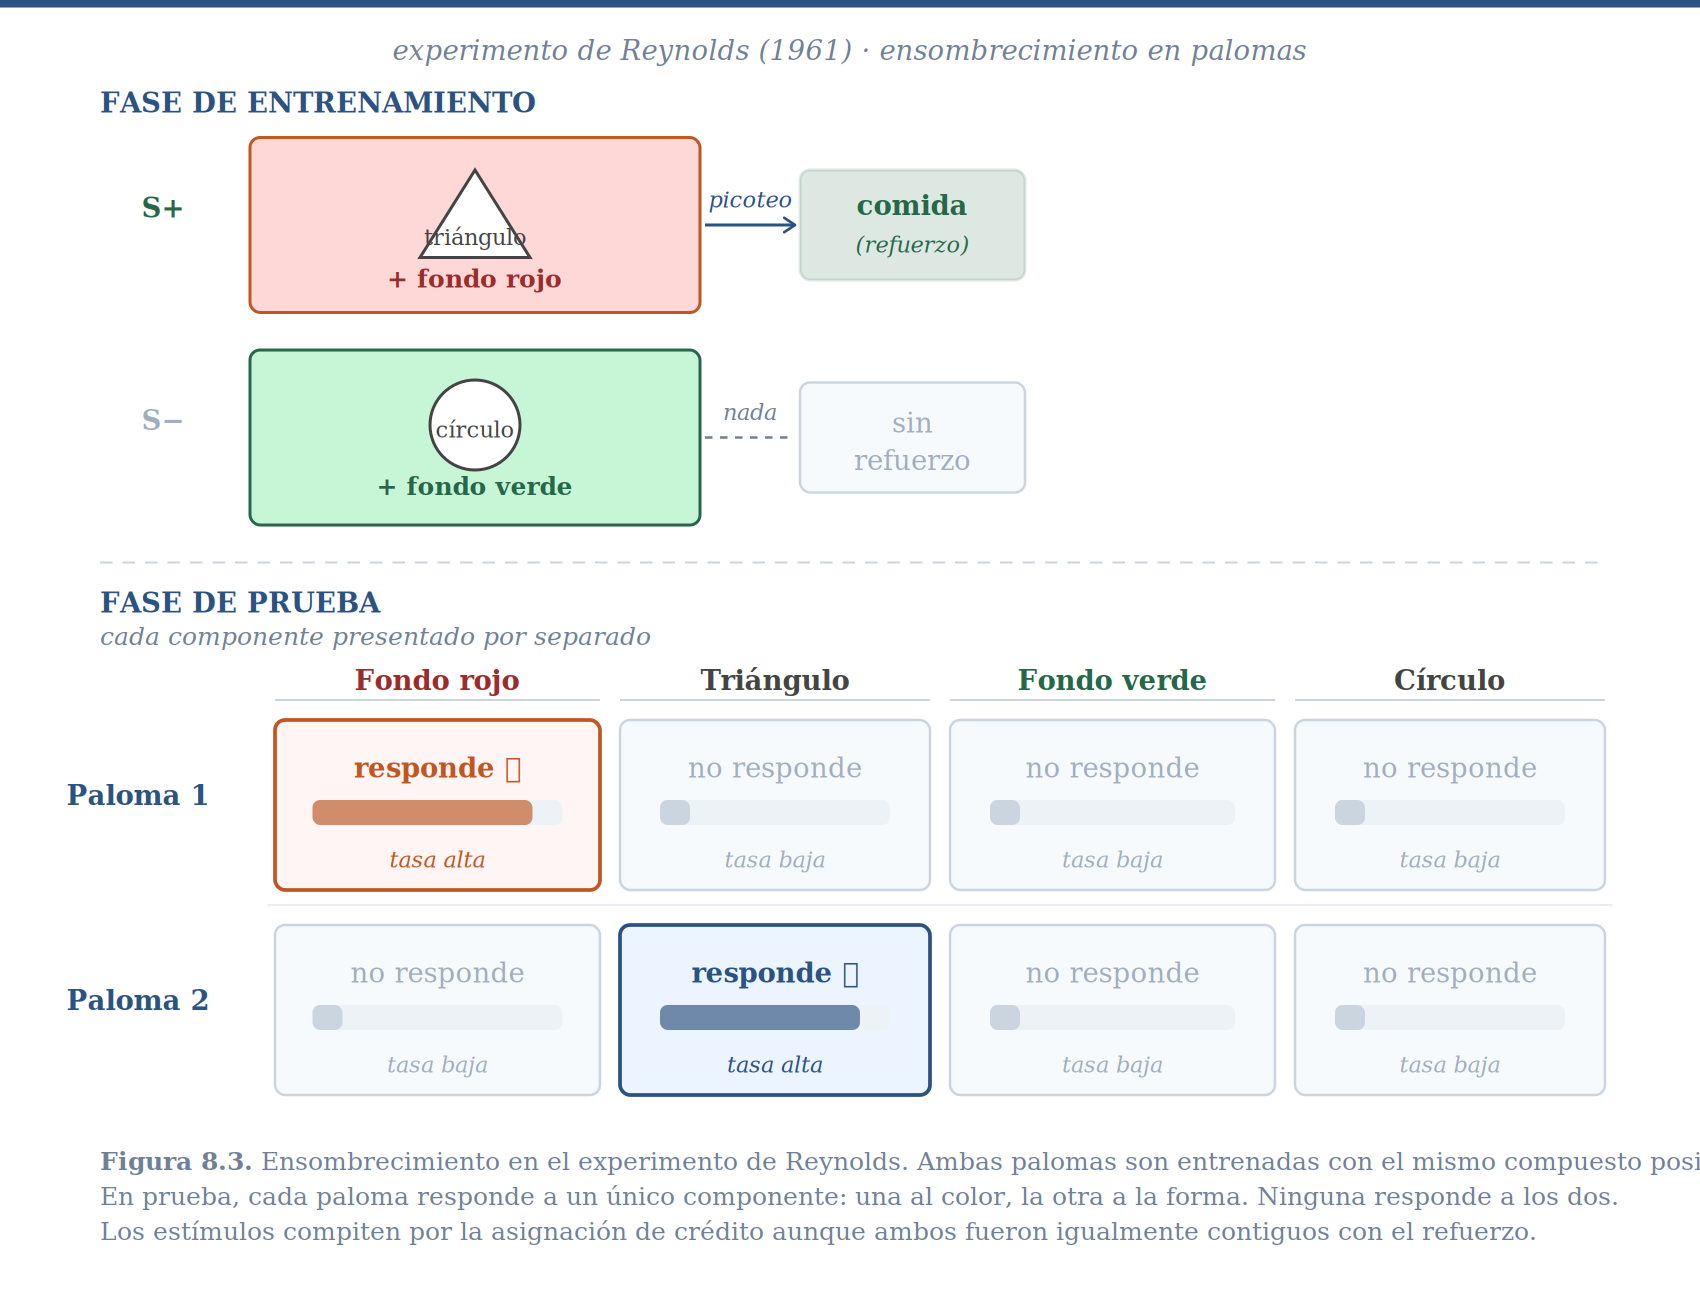
\includegraphics[width=0.9\linewidth,height=\textheight,keepaspectratio]{Figuras/fig8_3_ensombrecimiento.png}

}

\caption{\label{fig-reynolds}Ensombrecimiento en el experimento de
Reynolds (1961).}

\end{figure}%

\begin{quote}
\textbf{Note}

\textbf{Descripción.} Fase de entrenamiento: ambas palomas reciben el
mismo compuesto positivo (triángulo blanco sobre fondo rojo → comida) y
el mismo compuesto negativo (círculo blanco sobre fondo verde → nada).
Fase de prueba: cada componente se presenta por separado. La paloma 1
responde al fondo rojo pero no a la forma; la paloma 2 responde a la
forma triangular pero no al color. Ninguna responde a ambos componentes
del compuesto positivo, a pesar de que ambos fueron igualmente contiguos
con el refuerzo durante el entrenamiento. Los estímulos compiten por la
asignación de crédito.
\end{quote}

El resultado fue que cada paloma respondía a solo uno de los dos
componentes del compuesto positivo. Una paloma respondía al color rojo e
ignoraba la forma; la otra respondía a la forma triangular e ignoraba el
color. A pesar de que ambos elementos habían sido perfectamente
contiguos con la recompensa durante el entrenamiento, solo uno de ellos
adquirió control conductual en cada animal.

A este fenómeno se le llama \textbf{ensombrecimiento}: un elemento
saliente del compuesto ---más intenso, más novedoso, más contrastante---
``ensombrece'' el aprendizaje sobre elementos menos salientes. La
implicación es fundamental: los estímulos no aprenden en paralelo de
manera independiente. Compiten entre sí por la asignación de crédito. Lo
que aprende uno afecta lo que puede aprender el otro.

Retomando el ejemplo del perro amenazante: si el perro te ataca, para
algunos de ustedes el predictor establecido será el gruñido, para otros
el color del pelaje, para otros la raza. Los factores que determinan
cuál elemento gana la competencia incluyen la saliencia perceptual
---qué tan intenso o contrastante es el estímulo--- y las
predisposiciones de relevancia biológica que acabamos de discutir. Lo
que el ensombrecimiento establece es que esta competencia existe, y que
ganarla no es simplemente cuestión de ser contiguo con el suceso.

\subsection{Bloqueo: La Historia del Organismo
Importa}\label{bloqueo-la-historia-del-organismo-importa}

Si el ensombrecimiento muestra que la contigüidad no basta cuando dos
estímulos compiten simultáneamente, el experimento de bloqueo de Leon
Kamin demuestra algo más llamativo: la historia previa de un estímulo
puede suprimir completamente el aprendizaje sobre otro estímulo, incluso
cuando ambos son igualmente contiguos con el suceso biológicamente
importante.

El punto se entiende bien con un ejemplo cotidiano. Imagina que después
de visitar varios restaurantes has aprendido que los manteles de tela
son un buen predictor de la calidad de la comida. Visitas ahora un
restaurante nuevo que tiene manteles de tela y, además, música clásica
de fondo. La comida es igualmente buena. ¿Habrás aprendido que la música
clásica predice buena comida? Para saberlo tendrías que observar si, al
elegir entre dos restaurantes nuevos sin manteles de tela, preferirías
el que tiene música clásica. La intuición sugiere que probablemente no.
Una vez que el mantel de tela ya predecía perfectamente la buena comida,
la música clásica no añadía información nueva.

Leon Kamin puso a prueba esta intuición en 1969 en uno de los
experimentos más influyentes en la historia del estudio del aprendizaje.
El diseño trabajó con dos grupos de ratas. Al grupo experimental se le
entrenó primero con luz sola seguida de descarga eléctrica, hasta que la
luz era un predictor establecido. Luego, ese mismo grupo recibió
presentaciones del compuesto luz más tono seguido de descarga. Al grupo
control, se le presentó el compuesto desde el inicio, sin la fase previa
con la luz. En ambos casos, la tercera fase consistió en presentar el
tono solo para medir cuánto habían aprendido las ratas sobre él.

\begin{figure}[H]

\centering{

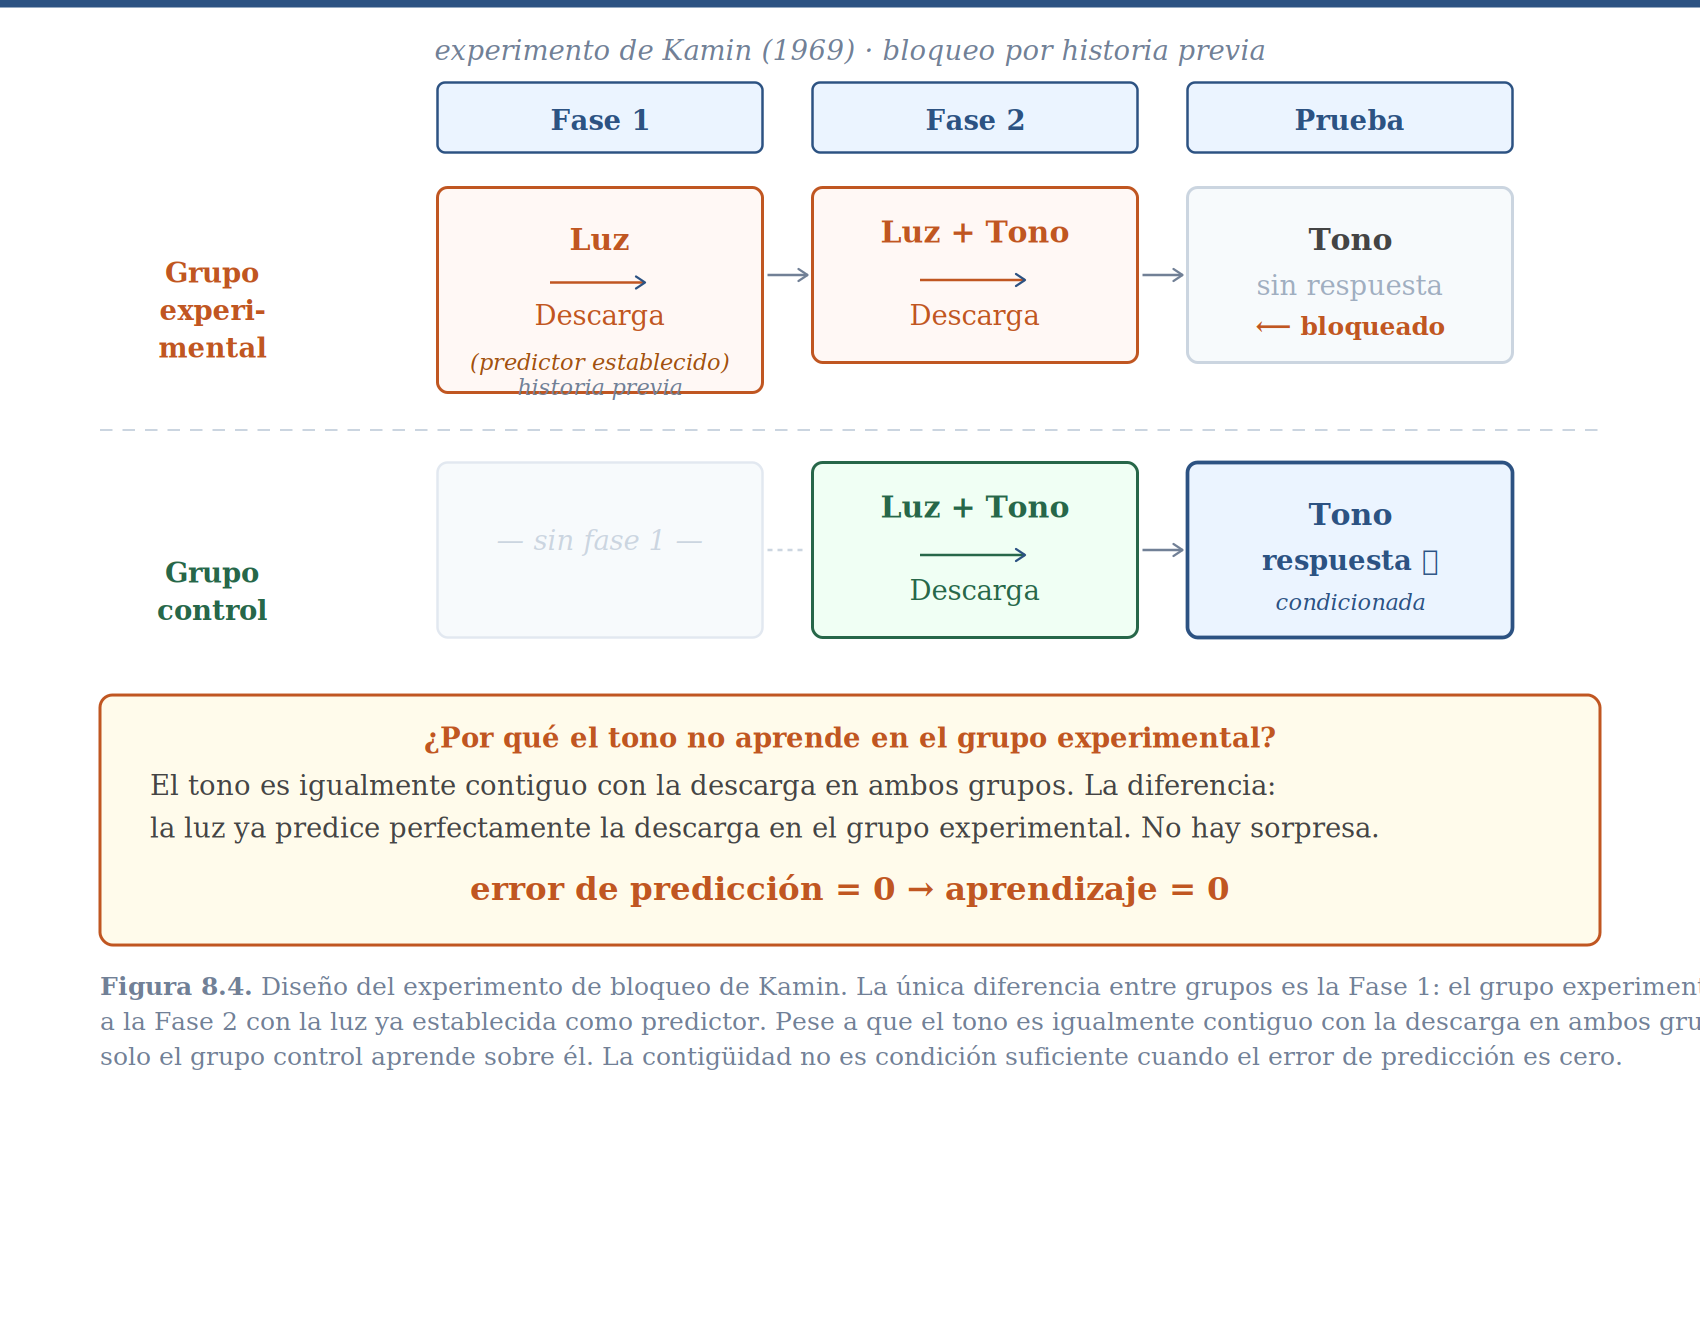
\includegraphics[width=0.9\linewidth,height=\textheight,keepaspectratio]{Figuras/fig8_4_bloqueo_kamin.png}

}

\caption{\label{fig-kamin}Diseño del experimento de bloqueo de Kamin
(1969).}

\end{figure}%

\begin{quote}
\textbf{Note}

\textbf{Descripción.} La única diferencia entre grupos es la Fase 1: el
grupo experimental llega a la Fase 2 con la luz ya establecida como
predictor de la descarga; el grupo control no tiene historia previa. En
la Fase 2 ambos grupos reciben el compuesto luz+tono seguido de
descarga. En la prueba, solo el grupo control muestra respuesta
condicionada al tono. El tono es igualmente contiguo con la descarga en
ambos grupos --- la diferencia es que en el grupo experimental la luz ya
predice perfectamente la descarga, el error de predicción es cero, y no
hay nada nuevo que aprender.
\end{quote}

Los resultados fueron claros. Las ratas del grupo control ---que no
tenían experiencia previa con la luz--- aprendieron a responder al tono.
Las del grupo experimental ---cuya luz ya era un predictor
establecido--- no mostraron prácticamente ningún aprendizaje sobre el
tono. El término para este fenómeno es \textbf{bloqueo}: la experiencia
previa con un predictor establecido bloquea el aprendizaje sobre nuevos
estímulos incorporados al compuesto.

¿Por qué ocurre el bloqueo? La interpretación que el experimento sugiere
es que las ratas del grupo experimental, al encontrar el compuesto luz
más tono seguido de descarga, no se sorprenden: la luz ya predecía la
descarga. No hay nada nuevo que aprender. El tono es informacionalmente
redundante ---su presencia o ausencia no modifica la predictibilidad del
suceso. Y si no hay información nueva, no hay razón para modificar el
sistema.

Esta interpretación revela algo profundo sobre la lógica del
aprendizaje: el sistema no responde a la mera ocurrencia del suceso
biológicamente importante, sino a la \emph{sorpresa} que ese suceso
produce. El aprendizaje es proporcional a la discrepancia entre lo que
ocurrió y lo que se esperaba. Si la predicción era perfecta, el error es
cero y no hay aprendizaje. Si ocurre algo inesperado, el error es
distinto de cero y el sistema se actualiza. Kamin llamó a esta idea
predictibilidad; en el capítulo siguiente la veremos formalizada con
precisión matemática como \textbf{error de predicción}.

\section{Optimalidad: ¿Cuándo Funciona la Contigüidad y Cuándo
Falla?}\label{optimalidad-cuuxe1ndo-funciona-la-contiguxfcidad-y-cuuxe1ndo-falla}

Hemos descrito la contigüidad como un sesgo inductivo y hemos dicho que
es el resultado de aprendizaje filogenético. Conviene ahora preguntarse
con más precisión cuándo es una política óptima y cuándo no.

Un sesgo es óptimo cuando la estructura del entorno para el que fue
diseñado coincide con la estructura del entorno donde se aplica. La
contigüidad temporal como heurística para causalidad funciona bien
cuando los mecanismos causales biológicamente relevantes producen sus
efectos con rapidez. Considera los casos más frecuentes en el entorno
ancestral de la mayoría de los animales: un depredador que ataca produce
dolor en segundos; un alimento que desencadena saciedad lo hace en
minutos; una pareja potencial que emite una señal está presente cuando
la emite. En estos contextos, la relación causal tiene una firma
temporal característica: el efecto sigue a la causa con relativa
inmediatez.

En esos entornos, la contigüidad es una heurística potente porque
permite ignorar la inmensa mayoría del historial de eventos pasados y
concentrar la búsqueda en los candidatos temporalmente recientes. El
costo de ignorar candidatos lejanos en el tiempo es bajo, porque causas
lejanas son improbables dado el tipo de mecanismos que operan.

Pensemos en el parámetro que controla la anchura del gradiente de la
demora ---qué tan rápido declina el aprendizaje conforme aumenta el
intervalo entre estímulo y consecuencia. En los experimentos
pavlovianos, ese parámetro está calibrado para intervalos de segundos a
minutos. Esa calibración no es arbitraria: refleja la distribución real
de demoras causales en el entorno ancestral. Un organismo con un
gradiente demasiado estrecho ---que solo aprende sobre eventos del
último segundo--- pierde muchas relaciones causales reales. Uno con un
gradiente demasiado amplio ---que considera como candidatos todo lo que
ocurrió en la última semana--- incluye tanto ruido que el espacio de
candidatos vuelve a ser inmanejable. El valor óptimo está en algún punto
entre estos extremos, y ese punto depende de la distribución de demoras
causales en el entorno.

El experimento de García es el contraejemplo perfecto al parámetro
estándar. Las toxinas que producen malestar gastrointestinal tienen
perfiles temporales peculiares: muchos venenos naturales requieren horas
para ser absorbidos y producir síntomas. Un organismo cuyo gradiente de
demora solo cubriera minutos sería incapaz de aprender a evitar la
mayoría de los alimentos tóxicos en la naturaleza. La selección natural
resolvió esto de manera elegante: para la clase específica de relación
sabor-malestar gastrointestinal, el gradiente de la demora es mucho más
ancho que para otras relaciones causales. Esto no contradice el
principio general de la contigüidad ---lo especializa: la anchura óptima
del gradiente depende del mecanismo causal específico que se está
detectando.

El sesgo de relevancia biológica opera, en este sentido, en dos niveles
simultáneos. Por un lado, define qué dimensiones del estímulo son
siquiera candidatos para la asignación de crédito dado el tipo de
consecuencia: sabores para el malestar gastrointestinal en omnívoros,
señales visuales para el dolor externo. Por otro, calibra la anchura del
gradiente de demora para cada tipo de relación: estrecho donde el
mecanismo causal es rápido ---depredador y dolor---, amplio donde es
lento ---toxina y malestar---. Y el sistema nervioso ha sido construido
para que esta calibración diferencial ocurra de manera automática,
dependiendo del tipo de suceso biológicamente importante que activa el
sistema de comportamiento relevante.

Nótese que esta es exactamente la lógica de los pasajes de optimalidad
de los capítulos anteriores: el parámetro que controla la sensibilidad
al error ---\emph{b} en kinesis, \emph{k} en taxias--- tiene un valor
óptimo que depende del entorno, y la solución verdaderamente óptima es
poder ajustar ese valor adaptativamente. La anchura del gradiente de la
demora es otro parámetro con esta misma propiedad. La selección natural
lo ha ajustado de manera diferenciada para diferentes clases de
relaciones causales, pero ese ajuste es fijo para cada especie. El
aprendizaje individual puede, dentro de ciertos límites, afinar esa
calibración a las condiciones específicas del entorno del organismo.

\begin{itemize}
\tightlist
\item
\end{itemize}

\emph{Básico.} Antes de correr el simulador, predice: ¿a qué intervalo
habrá caído la fuerza de condicionamiento a la mitad en cada
preparación? Verifica tu predicción con el gráfico. (Pista: cuando
exp(−t/τ) = 0.5, despeja t.)

\emph{Intermedio.} Modifica \texttt{tau\_pavlov} a 5, 15 y 60 segundos.
Para cada valor, describe el tipo de entorno ---¿qué clase de mecanismos
causales predominan?--- que haría óptimo ese gradiente. ¿Qué costo paga
el organismo con un tau demasiado estrecho? ¿Y con uno demasiado amplio?

\emph{Avanzado.} Diseña una ``especie'' con dos parámetros tau
independientes: uno estrecho para relaciones audiovisuales y uno amplio
para relaciones gustativas. ¿Cuándo y por cuánto supera la especie
especializada a la generalista?

\begin{center}\rule{0.5\linewidth}{0.5pt}\end{center}

\emph{Básico.} En el escenario de bloqueo, el estímulo B es tan contiguo
con el EI como el estímulo A durante la Fase 2. ¿Por qué no aprende?
Observa el valor de la variable \texttt{error} al inicio de la Fase 2 y
explica qué ocurre con él.

\emph{Intermedio.} Modifica el experimento de bloqueo de modo que
\texttt{lam} cambie de 1.0 a 1.5 en la Fase 2 ---el EI se vuelve más
intenso. ¿Qué ocurre ahora con B? Este resultado tiene un nombre en la
literatura experimental (el ``desbloqueo''). ¿Por qué tiene sentido
desde la perspectiva del error de predicción?

\emph{Avanzado.} El ensombrecimiento depende de la diferencia en
\texttt{alpha\_A} y \texttt{alpha\_B}. Encuentra el valor mínimo de esa
diferencia para que el ensombrecimiento sea ``completo'' ---es decir,
para que B aprenda menos del 10\% del máximo posible. ¿Cómo depende ese
umbral del valor de \texttt{beta}? ¿Qué dice esto sobre la interacción
entre saliencia del estímulo y tasa de aprendizaje del EI?

\begin{center}\rule{0.5\linewidth}{0.5pt}\end{center}

\section{Hacia el Modelo Formal}\label{hacia-el-modelo-formal}

Los experimentos de Pavlov, García, Reynolds y Kamin describen, en
conjunto, un sistema de aprendizaje con propiedades precisas. Es
sensible a la contigüidad, pero no esclavamente. Está modulado por la
relevancia biológica del suceso. Procesa estímulos en competencia, no de
manera independiente. Y su motor no es la mera co-ocurrencia de un
estímulo con un suceso, sino la información que ese estímulo aporta
sobre la predicción de ese suceso.

Estos hechos no son una colección de curiosidades ---son las
restricciones que debe satisfacer cualquier modelo formal del
aprendizaje asociativo. El bloqueo, en particular, plantea un desafío
conceptual preciso: ¿por qué un estímulo contiguo con un suceso
biológicamente importante no aprende nada, si ese suceso ocurrió? La
respuesta que los experimentos sugieren es que el sistema no responde a
la ocurrencia del suceso ---responde a la \emph{sorpresa} que ese suceso
produce. Si el suceso ya estaba predicho, su ocurrencia no es
sorprendente y no hay información nueva que incorporar. El tono no
aprende en el experimento de Kamin porque el error de predicción es
cero: la luz ya predecía perfectamente la descarga, y la descarga
ocurrió exactamente como se esperaba.

Esta intuición se formaliza de manera precisa en el modelo propuesto por
Bush y Mosteller en 1951, que estudiaremos en el capítulo siguiente. El
modelo parte de una idea simple: lo que controla el aprendizaje no es el
valor absoluto del suceso biológicamente importante, sino la
discrepancia entre el suceso obtenido y el suceso predicho ---el error
de predicción. Cuando la predicción es perfecta, el error es cero y no
hay aprendizaje. Cuando hay sorpresa, el error es distinto de cero y el
sistema se actualiza.

Noten la conexión con lo que ya conocen. El error de predicción es la
misma operación que la señal de error en los sistemas de
retroalimentación del capítulo 5: la discrepancia entre el estado
deseado y el estado actual. Y es la misma operación que aparece en la
ecuación de Price: la diferencia entre el rasgo del individuo y el
promedio de la población, ponderada por el éxito relativo. El mismo
principio reaparece ahora en el aprendizaje asociativo. El capítulo
siguiente formaliza ese principio y muestra cómo una ecuación
sorprendentemente simple captura el ensombrecimiento, el bloqueo, la
extinción y docenas de otros fenómenos del condicionamiento clásico.

\begin{center}\rule{0.5\linewidth}{0.5pt}\end{center}

\section{Conexiones}\label{conexiones-1}

\subsection{Hacia atrás: Selección Natural y
Retroalimentación}\label{hacia-atruxe1s-selecciuxf3n-natural-y-retroalimentaciuxf3n}

Los sesgos inductivos son el resultado directo del proceso que
describimos en el capítulo sobre selección natural. El genoma, actuando
como archivo causal acumulado a lo largo de generaciones, codifica las
regularidades estadísticas del entorno ancestral en forma de
predisposiciones a aprender ciertas relaciones más fácilmente que otras.
La ecuación de Price es el mecanismo mediante el cual esos sesgos fueron
refinados: los organismos con sesgos mejor calibrados al entorno dejaron
más descendientes, y esa covarianza entre el sesgo y el éxito
reproductivo produjo el ajuste acumulativo que observamos hoy.

La señal de error en los sistemas de retroalimentación ---la
discrepancia entre el set point y el valor actual--- es la misma
operación que ahora reaparece como error de predicción: la discrepancia
entre lo que el organismo esperaba y lo que ocurrió. La arquitectura es
la misma; cambia el tipo de variable que se compara.

\subsection{Hacia adelante: Asignación de Crédito a Respuestas (Capítulo
9)}\label{hacia-adelante-asignaciuxf3n-de-cruxe9dito-a-respuestas-capuxedtulo-9}

El problema que hemos abordado en este capítulo es la asignación de
crédito a estímulos: ¿qué eventos del entorno predicen el suceso
biológicamente importante? El capítulo 9 plantea el problema análogo
para respuestas: ¿qué acciones del organismo \emph{producen} ese suceso?
Los principios son estructuralmente similares ---contigüidad,
relevancia, novedad, competencia--- pero el hecho de que el organismo
mismo genera la variabilidad sobre la que opera la selección introduce
complejidades adicionales. El trabajo de Staddon y Simmelhag que veremos
en ese capítulo conecta directamente con la teoría de sistemas de
comportamiento introducida aquí.

\subsection{Hacia adelante: Bush y Mosteller y el Error de Predicción
(Capítulo
10)}\label{hacia-adelante-bush-y-mosteller-y-el-error-de-predicciuxf3n-capuxedtulo-10}

El bloqueo de Kamin establece la evidencia central que motiva el primer
modelo formal del aprendizaje asociativo. El aprendizaje no responde a
la ocurrencia del suceso biológicamente importante sino a la
\emph{sorpresa} que ese suceso produce ---la discrepancia entre lo que
ocurrió y lo que el organismo esperaba. En 1951, Bush y Mosteller
formalizaron esa intuición en una ecuación de actualización cuya
estructura es simple: el valor de un estímulo se ajusta en cada ensayo
en proporción a esa discrepancia. La velocidad del ajuste está
controlada por un parámetro α que cumple la misma función que \emph{b}
en kinesis y \emph{k} en taxias: determinar qué tanto le importa al
sistema la diferencia entre predicción y resultado. El capítulo 8
desarrolla ese modelo a partir de los datos sobre aprendizaje de
estímulos que hemos visto aquí.

\subsection{Hacia adelante: Rescorla-Wagner y la Competencia entre
Estímulos (Capítulo
11)}\label{hacia-adelante-rescorla-wagner-y-la-competencia-entre-estuxedmulos-capuxedtulo-11}

El modelo de Bush y Mosteller captura el error de predicción para un
estímulo en solitario, pero no deriva el bloqueo. El bloqueo requiere
algo adicional: que el error de predicción no se calcule sobre el valor
de un estímulo individual sino sobre la suma de los valores de
\emph{todos} los estímulos presentes simultáneamente. Esa extensión
---propuesta por Rescorla y Wagner en 1972--- convierte la competencia
entre estímulos en una consecuencia matemática de la ecuación, no en un
supuesto adicional. Cuando A ya predice perfectamente el suceso
biológicamente importante, la suma de valores iguala al máximo posible,
el error es cero, y B no aprende nada aunque sea perfectamente contiguo.
El capítulo 11 examina ese modelo y sus consecuencias, que van bastante
más lejos del bloqueo.

\begin{center}\rule{0.5\linewidth}{0.5pt}\end{center}

\section{Resumen}\label{resumen-2}

El problema de la asignación de crédito pregunta cuál de los
innumerables eventos que preceden a un suceso biológicamente importante
merece ser identificado como su predictor. El espacio de candidatos es
enorme, y sin guía la búsqueda es computacionalmente intratable.

Los organismos resuelven este problema con una cascada de sesgos
inductivos que operan en distintos niveles. El primer filtro lo
proporcionan los sistemas de comportamiento: el tipo de suceso
biológicamente importante activa el sistema funcionalmente apropiado, y
ese sistema determina qué dimensiones del entorno son siquiera
relevantes. Dentro del sistema activo, la contigüidad temporal opera
como primer sesgo: los eventos cercanos en el tiempo son candidatos
prioritarios porque la mayoría de los mecanismos causales biológicamente
relevantes operan con rapidez. La relevancia biológica especifica
adicionalmente qué dimensiones del estímulo ---sabor, sonido, imagen---
son más probables de ser causalmente relevantes para cada tipo de
consecuencia, reflejando la historia evolutiva de la especie en su nicho
ecológico particular. La novedad prioriza estímulos nuevos sobre
familiares, porque causas nuevas son más plausibles para efectos nuevos.

Pero la contigüidad no es ni necesaria ni suficiente. No es necesaria
porque las aversiones al sabor demuestran que se puede aprender con
demoras de horas. No es suficiente porque el ensombrecimiento y el
bloqueo demuestran que la contigüidad no garantiza aprendizaje cuando
hay competencia entre estímulos. El principio subyacente, que el bloqueo
de Kamin revela con especial claridad, es que el aprendizaje no es
proporcional a la ocurrencia del suceso sino a la sorpresa que ese
suceso produce ---la discrepancia entre lo que ocurrió y lo que el
organismo esperaba. Esa discrepancia es el error de predicción, concepto
que los capítulos 8 y 9 formalizarán en dos pasos: primero para
estímulos individuales, luego para estímulos en competencia.

\begin{center}\rule{0.5\linewidth}{0.5pt}\end{center}

\section{Ejercicios}\label{ejercicios}

\textbf{1.} El capítulo propone que los sesgos inductivos son
``conocimiento filogenético sobre la estructura causal del mundo''.
Explica con tus propias palabras qué significa esto. ¿Qué tendría que
haber sido cierto en el entorno ancestral de los roedores omnívoros para
que el sesgo de relevancia biológica gustativa ---buscar la causa del
malestar gastrointestinal en los sabores recientes--- haya evolucionado?
¿Qué tipo de entorno haría desadaptativo ese mismo sesgo?

\textbf{2.} El experimento de García usó un compuesto de sabor +
estímulo audiovisual. Las ratas con malestar gastrointestinal
aprendieron a evitar el sabor pero no el estímulo audiovisual; las ratas
con descarga eléctrica hicieron lo contrario. Reformula este resultado
en términos de sistemas de comportamiento: ¿qué sistema activa cada tipo
de consecuencia, y cómo determina ese sistema qué dimensiones del
estímulo entran en el espacio de candidatos? En el grupo de descarga,
ambos componentes del compuesto eran igualmente contiguos con el shock;
en el grupo de enfermedad, la consecuencia llegó horas después. ¿Cambia
esta asimetría de demoras la interpretación del resultado en términos de
sistemas de comportamiento, o el fenómeno es el mismo independientemente
de la demora? Justifica tu respuesta.

\textbf{3.} El gradiente de la demora tiene un valor óptimo que depende
del tipo de mecanismo causal. Para cada uno de los siguientes pares
causa-efecto, razona cuál sería el rango de demoras que debería cubrir
el gradiente óptimo, y por qué: (a) depredador → ataque, (b) toxina de
digestión lenta → malestar, (c) pareja potencial → apareamiento. ¿Qué
predice este análisis sobre las diferencias entre especies con dietas o
nichos ecológicos distintos?

\textbf{4.} En el experimento de bloqueo de Kamin, el grupo control
aprende sobre el tono aunque el tono es igualmente contiguo con la
descarga para ambos grupos. Usa el concepto de error de predicción para
explicar por qué el grupo control aprende y el experimental no. Luego
predice qué ocurriría si en la Fase 2 del experimento la descarga fuera
el doble de intensa que en la Fase 1. ¿Cambiaría el resultado para el
grupo experimental? ¿Por qué?

\textbf{5.} Usa el Simulador 6.2 para explorar qué ocurre cuando
\texttt{lam} cambia de 1.0 a 1.5 en la Fase 2 del bloqueo. Este
resultado, llamado ``desbloqueo'', fue una de las primeras evidencias
experimentales a favor del modelo de Rescorla-Wagner. Explica en
términos intuitivos ---sin la ecuación formal, que veremos en el
siguiente capítulo--- por qué el cambio en la intensidad del EI
``desbloquea'' el aprendizaje sobre el estímulo que había sido
bloqueado.

\textbf{6.} \emph{(Reflexión)} El capítulo afirma que los sesgos
inductivos son soluciones evolutivas a un problema computacional real,
no limitaciones arbitrarias. Pero también pueden producir errores
sistemáticos cuando el organismo se encuentra en un entorno diferente
del ancestral. Describe dos situaciones del entorno humano contemporáneo
en que los sesgos de contigüidad o relevancia biológica llevan a
conclusiones erróneas sobre la causalidad. ¿Qué tienen en común esas
situaciones? ¿Qué dice esto sobre el alcance y los límites del
aprendizaje filogenético?

\begin{center}\rule{0.5\linewidth}{0.5pt}\end{center}

\section{Lecturas Recomendadas}\label{lecturas-recomendadas}

\textbf{García, J., \& Koelling, R. A. (1966).} Relation of cue to
consequence in avoidance learning. \emph{Psychonomic Science, 4},
123--124. --- El artículo original en dos páginas. Imprescindible por su
claridad y porque el experimento habla por sí mismo.

\textbf{Kamin, L. J. (1969).} Predictability, surprise, attention, and
conditioning. En B. A. Campbell \& R. M. Church (Eds.), \emph{Punishment
and Aversive Behavior}. Appleton-Century-Crofts. --- El experimento
original del bloqueo con el análisis conceptual completo. Accesible y
con la lógica del experimento explicada paso a paso.

\textbf{Seligman, M. E. P. (1970).} On the generality of the laws of
learning. \emph{Psychological Review, 77}, 406--418. --- El artículo que
sistematizó la evidencia de relevancia biológica y acuñó el término
\emph{preparedness}. Vista panorámica más allá de los experimentos
individuales.

\textbf{Timberlake, W., \& Lucas, G. A. (1989).} Behavior systems and
learning: From misbehavior to general principles. En S. B. Klein \& R.
R. Mowrer (Eds.), \emph{Contemporary Learning Theories}. Erlbaum. --- La
exposición más accesible del enfoque de sistemas de comportamiento
aplicado al aprendizaje.

\textbf{Domjan, M. (2005).} Pavlovian conditioning: A functional
perspective. \emph{Annual Review of Psychology, 56}, 179--206. ---
Revisión de cómo los principios del condicionamiento reflejan soluciones
evolutivas a problemas adaptativos. Nivel moderado; muy recomendable
como lectura de integración después de este capítulo.

\begin{center}\rule{0.5\linewidth}{0.5pt}\end{center}

\bookmarksetup{startatroot}

\chapter{El Problema de la Asignación de Crédito
(II)}\label{el-problema-de-la-asignaciuxf3n-de-cruxe9dito-ii}

\section{Acciones, Inducción y el Problema del
Control}\label{acciones-inducciuxf3n-y-el-problema-del-control}

Al final del capítulo anterior dejamos al organismo en posesión de una
capacidad importante pero parcial: puede predecir cuándo va a llover
mirando el cielo, puede anticipar el ataque de un depredador al escuchar
su rugido, puede aprender que ciertos sabores preceden al malestar. Esa
capacidad predictiva tiene un valor enorme, pero tiene también un límite
preciso: el organismo no controla el cielo, no controla la presencia del
depredador, no controla los sabores que encuentra. Puede prepararse para
lo que viene, pero no puede alterar lo que viene.

Uno de los saltos más importantes en la historia evolutiva fue la
emergencia de mecanismos que, a través de la acción y la interacción con
el entorno, permiten a los organismos no solo predecir sino
\emph{controlar} la ocurrencia de sucesos biológicamente importantes. Un
organismo que aprende no solo que el cielo nublado anuncia lluvia, sino
que \emph{llevar paraguas} produce la consecuencia de llegar seco, ha
adquirido algo cualitativamente distinto. La lluvia sigue siendo
independiente de él; pero la consecuencia de llegar empapado ya no lo
es. Entre la acción del organismo y el resultado hay ahora una relación
de dependencia que puede ser aprendida, explotada y perfeccionada.

Este es el problema adaptativo que nos ocupa: ¿cómo aprende un organismo
que sus propias acciones producen sucesos biológicamente importantes? Y,
antes de eso, ¿de dónde vienen las acciones entre las que puede elegir?

\section{Thorndike y dos preguntas que se confundieron durante
décadas}\label{thorndike-y-dos-preguntas-que-se-confundieron-durante-duxe9cadas}

A principios del siglo XX, Edward Thorndike encerró gatos en cajas de
escape desde las que el animal podía salir accionando un cerrojo,
tirando de una cuerda o pisando una palanca. El patrón fue consistente:
al inicio los gatos tardaban mucho, probando un repertorio amplio de
respuestas antes de dar con la correcta por casualidad; con la
repetición, ese tiempo disminuía hasta que el animal accionaba el
dispositivo casi inmediatamente. Thorndike llamó a esto aprendizaje por
\emph{ensayo y error}.

Pero los datos contienen dos observaciones distintas. La primera: el
gato \emph{hace algo} al ser encerrado. No se queda inmóvil, no
selecciona al azar de toda la gama posible de movimientos de un cuerpo
en el espacio. Explora, araña, empuja, vocaliza ---respuestas apropiadas
a la situación de escape, no al cortejo ni a la alimentación. La
segunda: de ese repertorio inicial, el animal selecciona progresivamente
la respuesta que abre la caja. Son fenómenos distintos: uno sobre el
origen de la variabilidad conductual, otro sobre su selección.

La \emph{Ley del Efecto} de Thorndike intentó responderlos con el mismo
principio: \emph{una respuesta seguida de un estado de cosas
satisfactorio queda asociada con la situación y aumenta su probabilidad
futura}. La contigüidad temporal era, para Thorndike, tanto condición
suficiente como necesaria. Esa confusión costó décadas.

\section{El primer sesgo: la inducción de respuestas por el
SBI}\label{el-primer-sesgo-la-inducciuxf3n-de-respuestas-por-el-sbi}

Retomemos el lenguaje del capítulo anterior. Los sesgos inductivos que
hacen manejable el problema de la asignación de crédito operan en dos
niveles distintos. El primero delimita el espacio de candidatos: ¿qué
respuestas son siquiera consideradas? El segundo establece el orden de
prioridad dentro de ese espacio reducido: ¿cuál se evalúa primero?

La Ley del Efecto, como señalamos, se concentra casi exclusivamente en
el segundo nivel ---la contigüidad como criterio de selección--- y deja
sin respuesta la pregunta del primer nivel. ¿De dónde viene el
repertorio inicial de respuestas sobre el que opera la selección?

La respuesta emergió de una dirección que Thorndike no anticipó. La mera
presentación de un suceso biológicamente importante \emph{induce} en el
organismo un conjunto de respuestas características: las apropiadas para
interactuar con ese tipo de consecuencia. No son respuestas arbitrarias
del espacio motor completo, sino un subconjunto organizado
funcionalmente. La comida induce comportamientos de consumación y
búsqueda alimentaria. Una amenaza induce comportamientos de escape y
evitación. Un posible compañero reproductivo induce comportamientos de
cortejo. Como vimos en el capítulo 6, estas respuestas inducidas se
organizan en los sistemas de comportamiento que Hogan y Timberlake
describieron: el SBI activa el sistema funcionalmente apropiado, y ese
sistema pre-configura el espacio de respuestas candidatas.

Pero el sistema de comportamiento no actúa en el vacío. ¿Qué respuestas
quedan disponibles depende también de qué oportunidades de acción ofrece
el entorno físico en ese momento. Una paloma ante un comedero no ejecuta
el mismo conjunto de respuestas alimentarias que una paloma en campo
abierto, aunque el SBI sea idéntico. El entorno no es un telón de fondo
neutro: estructura activamente qué respuestas son posibles y cuáles no.
Piensen en cómo cambia su comportamiento al entrar a una biblioteca
frente a entrar a un gimnasio, aunque lleguen con el mismo objetivo. El
concepto de \emph{affordance} ---que exploraremos con detalle en
capítulos posteriores--- captura esta idea: las propiedades del entorno
que hacen posibles ciertas acciones y no otras. Por ahora basta notar
que el repertorio inducido no es solo función del SBI; es función del
SBI \emph{en ese entorno particular}.

Este principio de inducción fue reconocido tempranamente en la
literatura del aprendizaje pero tardó en articularse con precisión
formal. Volveremos a él cuando lleguemos a los programas de refuerzo y
la igualación. Por ahora, la observación empírica clave provino de un
experimento diseñado para examinar la explicación de Skinner sobre un
fenómeno curioso: la ``superstición'' en palomas.

\section{El experimento de Skinner y la réplica de Staddon y
Simmelhag}\label{el-experimento-de-skinner-y-la-ruxe9plica-de-staddon-y-simmelhag}

En 1948, Skinner publicó un experimento que se volvería célebre. A
palomas hambrientas se les presentaba comida cada quince segundos,
completamente independiente de su comportamiento. Y sin embargo, muchas
aves desarrollaron comportamientos estereotipados: una giraba en
círculos, otra movía la cabeza rítmicamente, otra se desplazaba en
diagonal. El comportamiento difería entre individuos.

La interpretación de Skinner fue directa: para cada paloma, alguna
respuesta había ocurrido accidentalmente inmediatamente antes de la
entrega de comida, y esa contigüidad accidental era suficiente para
fortalecerla. El animal no necesitaba detectar ninguna relación real
entre su conducta y el resultado; bastaba la proximidad temporal para
producir el aprendizaje. Para Skinner, la contigüidad temporal era el
mecanismo: un reforzador era ``contingente'' sobre una respuesta en el
único sentido de que la seguía en el tiempo. El experimento de
superstición era su demostración más limpia.

Staddon y Simmelhag no estuvieron de acuerdo, y en 1971 publicaron una
réplica que cambiaría la discusión. Usaron el mismo procedimiento básico
de Skinner ---comida cada quince segundos independiente del
comportamiento--- pero observaron cuidadosamente qué hacían las palomas
\emph{a lo largo de todo el intervalo}, no solo en el momento
inmediatamente anterior a la comida. Los resultados desmontaron la
narrativa de Skinner en dos frentes.

Primero, el comportamiento no difería arbitrariamente entre palomas: era
predecible. Al final del intervalo, cerca del momento de entrega de la
comida, prácticamente todas las palomas mostraban el mismo tipo de
respuestas ---orientarse hacia la pared del comedero, picotear en esa
dirección. Staddon y Simmelhag llamaron a estas ``respuestas
terminales''. Inmediatamente después de recibir la comida, y durante la
primera mitad del intervalo siguiente, aparecían respuestas muy
distintas ---explorar el piso, dar giros, desplazarse--- que estos
autores llamaron ``respuestas interinas''. La figura 7.1 muestra esta
distribución temporal con claridad.

\begin{figure}[H]

{\centering 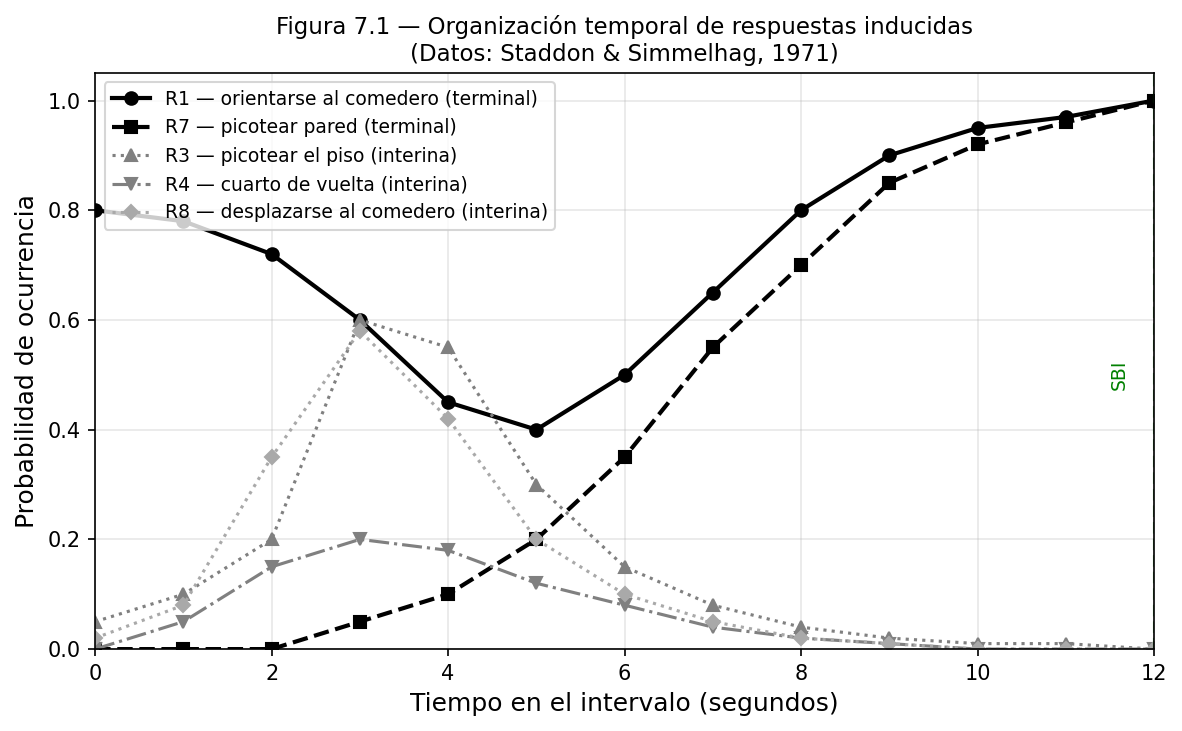
\includegraphics[width=7.8125in,height=\textheight,keepaspectratio]{Figuras/figura_9_1_staddon.png}

}

\caption{Organización temporal de respuestas inducidas}

\end{figure}%

\begin{quote}
\textbf{Note}

\textbf{Descripción.}Eje horizontal: tiempo en el intervalo entre
entregas de comida (0--12 seg). Eje vertical: probabilidad de
ocurrencia. Líneas sólidas negras: respuestas terminales (orientarse al
comedero, picotear la pared) --- crecen conforme se acerca el SBI y
alcanzan su máximo en t = 12. Líneas punteadas grises: respuestas
interinas (picotear el piso, dar giros, desplazarse) --- alcanzan su
máximo en la primera mitad del intervalo y declinan antes del SBI. Línea
vertical verde punteada: momento de entrega de comida. Datos de Staddon
y Simmelhag (1971).
\end{quote}

Segundo, el patrón no era el que predice la contigüidad accidental. Si
la contigüidad fuera el mecanismo, las respuestas que aparecen justo
antes de la comida ---las terminales--- deberían ser las que más varían
entre individuos, porque dependen de qué estaba haciendo cada paloma en
ese momento preciso por azar. Pero ocurrió exactamente lo contrario: las
respuestas terminales eran las más consistentes entre animales. Las
interinas, que ocurren lejos temporalmente de la comida, eran las que
mostraban más variación.

La conclusión fue clara: sin ninguna relación de dependencia entre
respuesta y comida, la mera contigüidad accidental no explicaba el
patrón observado. Lo que sí lo explicaba era el principio de inducción:
la presentación periódica de un SBI alimenticio induce el conjunto de
respuestas apropiadas para ese SBI, y la periodicidad temporal organiza
esas respuestas a lo largo del intervalo. Las terminales reflejan la
activación anticipatoria del sistema de alimentación conforme se acerca
el momento de la comida; las interinas son comportamientos de actividad
general inducidos por la llegada del SBI que van diluyéndose en el
tiempo. El comportamiento observado por Skinner no era aprendizaje por
contigüidad accidental ---era inducción organizada temporalmente. La
contigüidad, como condición suficiente para asignar crédito a una
respuesta, no se sostiene.

\section{¿Es la contigüidad una condición
necesaria?}\label{es-la-contiguxfcidad-una-condiciuxf3n-necesaria}

El experimento de Skinner eliminaba la relación de dependencia entre
respuesta y SBI. Los experimentos que siguen hacen lo contrario:
mantienen esa relación de dependencia pero manipulan la \emph{demora}
entre la respuesta y el SBI. Si la contigüidad fuera necesaria, una
demora suficientemente larga debería hacer imposible el aprendizaje. La
pregunta es cuánta demora puede tolerarse.

La estrategia experimental adoptó como punto de referencia la
contigüidad estricta ---demora de cero segundos--- y exploró qué ocurre
cuando ese intervalo se extiende progresivamente. Pero antes de
describir los resultados, conviene apreciar un problema metodológico que
hacía difícil interpretar estos experimentos con demora. Si el animal
puede seguir respondiendo durante el periodo de demora, sus respuestas
adicionales pueden quedar accidentalmente contiguas con el SBI que fue
producido por una respuesta anterior. ¿Cómo distinguir entonces si el
aprendizaje se debe a la relación de dependencia original ---la
respuesta que inició el contador--- o a esas contigüidades accidentales
posteriores?

Dickinson y sus colaboradores diseñaron un procedimiento que abordó
exactamente esta dificultad. Las ratas tenían una palanca disponible y
el tiempo de la sesión se dividía en intervalos de un segundo. En cada
segundo, el animal tenía la oportunidad de presionar la palanca. Cuando
lo hacía, se iniciaba un periodo de demora de duración programada, al
final del cual se entregaba la comida. El problema es que durante ese
periodo de demora el animal podía volver a presionar la palanca, y cada
nueva presión iniciaba un contador adicional ---lo que creaba la
posibilidad de que alguna presión quedara accidentalmente contigua con
la comida producida por una presión anterior.

Para resolver esta ambigüedad, Dickinson incluyó un segundo grupo de
ratas ---el grupo \emph{yoked} o apareado--- que recibía exactamente los
mismos refuerzos, en los mismos momentos, que el grupo experimental,
pero sin ninguna relación de dependencia entre su comportamiento y esa
entrega. Si el aprendizaje observado en el grupo experimental se debiera
solo a las contigüidades accidentales dentro del periodo de demora, el
grupo yoked debería aprender igual ---porque experimentaba las mismas
contigüidades accidentales, distribuidas del mismo modo en el tiempo. Si
el grupo experimental aprendía más, eso indicaba que la relación de
dependencia contribuía al aprendizaje más allá de las contigüidades
accidentales.

Con demoras de hasta dieciséis segundos, el grupo experimental aprendió
claramente; el grupo yoked no lo hizo. Con treinta y dos segundos, el
experimental seguía respondiendo más, aunque más lento. A sesenta y
cuatro segundos, ambos grupos fueron indistinguibles.

\begin{figure}[H]

{\centering 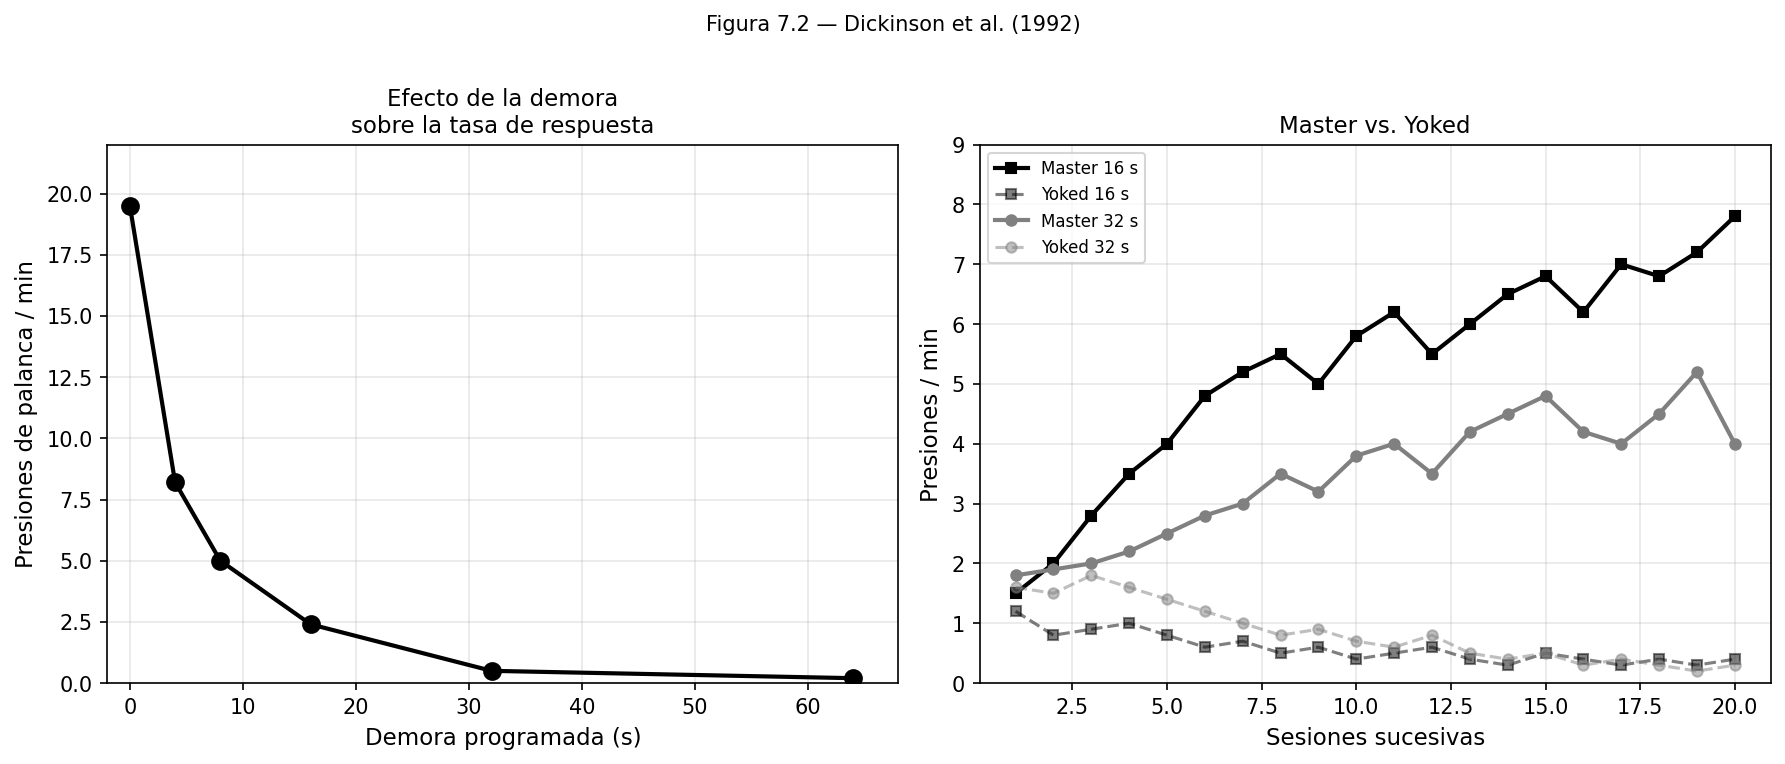
\includegraphics[width=7.8125in,height=\textheight,keepaspectratio]{Figuras/figura_9_2_dickinson.png}

}

\caption{Resultados de Dickinson et al.~(1992)}

\end{figure}%

\begin{quote}
\textbf{Note}

\textbf{Descripción}. Panel izquierdo: tasa de respuesta (presiones de
palanca por minuto) como función de la demora programada (0, 4, 8, 16,
32, 64 segundos) --- curva decreciente. Panel derecho: curvas de
adquisición para el grupo experimental (master) y el grupo apareado
(yoked) en condiciones de 16 y 32 segundos de demora. Las curvas del
grupo experimental crecen a lo largo de las sesiones; las del grupo
yoked permanecen en valores bajos. La disociación entre los dos grupos
demuestra que el aprendizaje se debe a la relación de dependencia, no a
contigüidades accidentales durante la demora. Datos de Dickinson et
al.~(1992).
\end{quote}

Hay dos conclusiones en estos datos. La primera es que la contigüidad
estricta no es necesaria: el organismo puede aprender la relación entre
su respuesta y la comida incluso cuando hay treinta y dos segundos entre
ellas, y ese aprendizaje no se debe a contigüidades accidentales sino a
la relación de dependencia en sí misma. La segunda es que la demora
importa: mientras más larga sea, más lento y débil es el aprendizaje. La
contigüidad no es la llave del aprendizaje, pero es un facilitador
poderoso.

Lattal fue aún más lejos en el experimento diseñado para eliminar
cualquier posibilidad de contigüidad accidental. Sus palomas recibían
comida, en promedio, cada treinta segundos ---pero solo si habían
transcurrido diez segundos desde la última respuesta. Si el animal
respondía antes de que pasaran esos diez segundos, el contador se
reiniciaba. Este procedimiento, conocido como DRO (\emph{differential
reinforcement of other behavior}), garantiza que la comida nunca puede
seguir inmediatamente a una respuesta: siempre habrá una separación
mínima de diez segundos. En ningún sentido ordinario del término puede
decirse que hay contigüidad entre respuesta y SBI.

Y sin embargo, las palomas de Lattal aprendieron. La tasa de picoteo de
la tecla aumentó claramente por encima de la línea base en cinco de los
cinco sujetos del experimento, como muestra la figura 7.3. El animal
aprendió a picar la tecla a pesar de que esa tecla nunca fue
inmediatamente seguida de comida ---a pesar de que, estrictamente
hablando, el procedimiento estaba diseñado para que hubiera una
separación garantizada. Si Dickinson mostró que la contigüidad no es
necesaria con demoras de decenas de segundos, Lattal mostró que no lo es
incluso cuando se elimina por diseño.

\begin{figure}[H]

{\centering 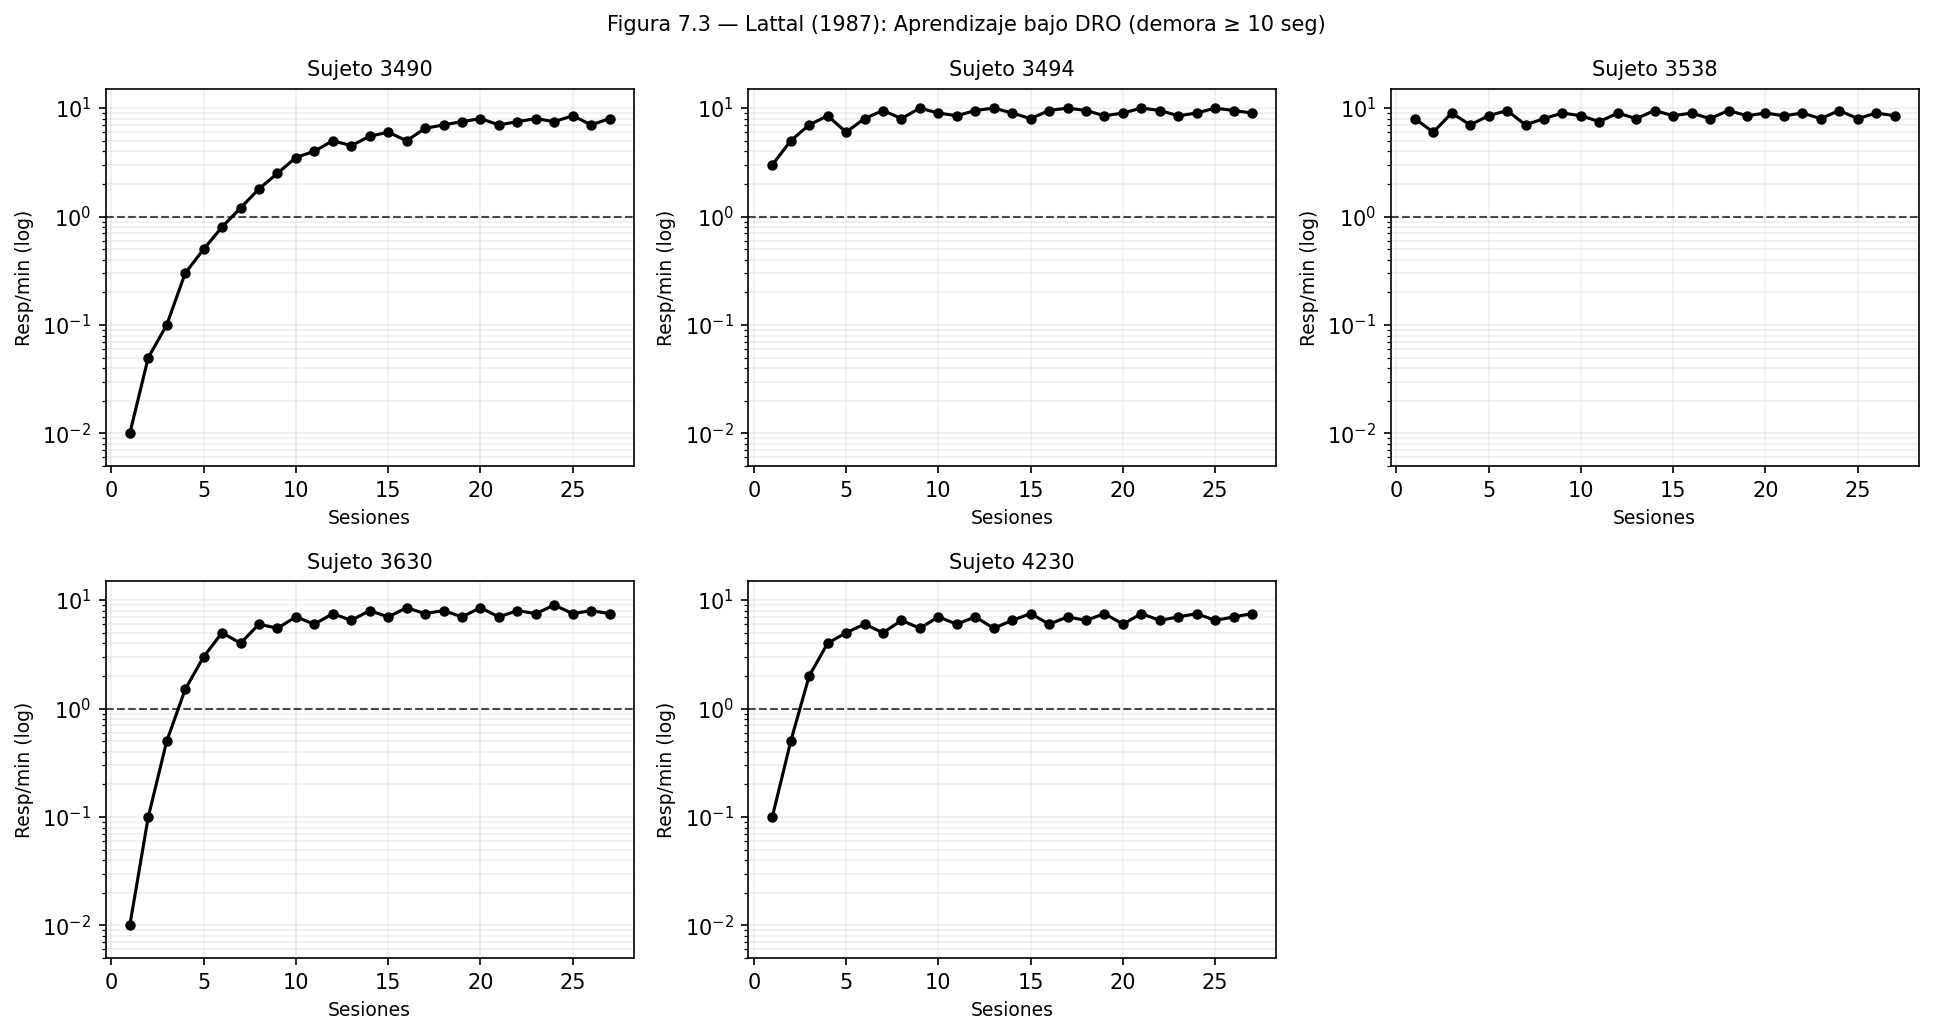
\includegraphics[width=7.8125in,height=\textheight,keepaspectratio]{Figuras/figura_9_3_lattal.png}

}

\caption{Resultados de Lattal (1987)}

\end{figure}%

\begin{quote}
\textbf{Note}

\textbf{Descripción} . Cinco paneles, uno por sujeto (palomas 3490,
3494, 3538, 3630, 4230). Eje horizontal: sesiones sucesivas. Eje
vertical: tasa de respuesta en escala logarítmica. Línea punteada
horizontal: tasa de referencia. En todos los sujetos la tasa de picoteo
aumenta claramente por encima de la línea de referencia a pesar de que
el procedimiento DRO garantizaba una separación mínima de 10 segundos
entre cualquier respuesta y la comida. Datos de Lattal (1987).
\end{quote}

La misma conclusión a la que llegamos en el capítulo anterior para los
estímulos se aplica aquí para las respuestas. Ni necesaria ni suficiente
---pero no irrelevante. Lo que los organismos hacen, más que registrar
proximidad temporal entre eventos discretos, es detectar una relación
estadística a lo largo del tiempo: que la tasa de SBIs es mayor cuando
cierta respuesta ocurre que cuando no ocurre. La contigüidad es un
correlato frecuente de esa relación causal real, y por eso sirve como
heurístico útil en muchas circunstancias. Pero no es la relación causal
misma.

\section{Perspectiva molecular y perspectiva
molar}\label{perspectiva-molecular-y-perspectiva-molar}

Este cambio de énfasis ---de eventos individuales a relaciones
estadísticas--- tiene un nombre en la literatura: es el contraste entre
las perspectivas molecular y molar del aprendizaje instrumental.

La perspectiva molecular examina pares de eventos individuales: esta
respuesta fue seguida de este SBI a tal distancia temporal. Es la
perspectiva que subyace a la idea de contigüidad: lo que importa es la
proximidad de cada par de eventos. La perspectiva molar, en cambio,
examina la covariación entre patrones de actividad y tasas de resultados
a lo largo de períodos extendidos: ¿cuál es la tasa de SBIs durante los
períodos en que el organismo ejecuta esta respuesta, comparada con la
tasa durante los períodos en que no la ejecuta?

La evidencia de Dickinson y Lattal habla a favor del nivel molar como el
nivel apropiado de análisis. El organismo no parece llevar un registro
de pares respuesta-SBI; parece integrar información sobre covariaciones
a lo largo de ventanas temporales amplias. Esta integración es lo que
hace posible el aprendizaje con demoras de decenas de segundos: la
demora individual entre respuesta y consecuencia no destruye el
aprendizaje porque la covariación estadística persiste a escalas de
tiempo más largas.

Veremos esta distinción reaparecer con más fuerza cuando lleguemos al
tema de los programas de refuerzo y la igualación, donde las teorías
moleculares predicen patrones de respuesta constantes dentro del
intervalo, mientras que las teorías molares predicen que lo que el
organismo maximiza es la tasa de SBIs a lo largo de períodos extendidos
---predicciones que divergen de manera empíricamente resoluble.

\section{La percepción de causalidad: el experimento de
Killeen}\label{la-percepciuxf3n-de-causalidad-el-experimento-de-killeen}

Hasta aquí hemos argumentado que los organismos son sensibles a la
covariación estadística entre sus respuestas y los SBIs. Pero ¿cómo
sería posible demostrarlo directamente, en lugar de inferirlo de los
experimentos de demora? Killeen diseñó una manera ingeniosa.

Sus palomas tenían ante sí una tecla central iluminada. Podían
picotearla, y con una probabilidad de 0.05, ese picotazo apagaba la
tecla central y encendía dos teclas laterales. Hasta aquí, un
procedimiento de aprendizaje ordinario. Pero Killeen añadió un elemento
crucial: al mismo tiempo que las palomas picoteaban, una computadora
generaba ``pseudo-picotazos'' a la misma tasa, y esos pseudo-picotazos
tenían también una probabilidad de 0.05 de apagar la tecla central.

En cualquier momento en que la tecla central se apagaba, podía haber
ocurrido por una de dos razones: porque la paloma acababa de picarla, o
porque la computadora generó un pseudo-picotazo. La tarea para las
palomas era discriminar entre estas dos posibilidades. Si el apagado lo
había causado su propio picotazo, picar la tecla derecha producía acceso
a comida. Si el apagado era independiente de su respuesta, picar la
tecla izquierda producía comida. Acertar ---identificar correctamente
que el apagado fue consecuencia del picotazo propio--- se llama un
\emph{acierto} o \emph{hit}. Confundir un apagado independiente con uno
causado por la propia respuesta se llama \emph{falsa alarma}.

Lo que hace este diseño particularmente poderoso es que permite separar
dos cosas que normalmente van juntas: la capacidad real para detectar
causalidad, y el criterio de decisión que el organismo adopta dados los
pagos asociados a acertar y equivocarse. Killeen varió la cantidad de
comida que las palomas recibían tras un acierto, manteniendo constante
el costo de las falsas alarmas.

El primer resultado fue que las palomas son detectoras genuinas de
causalidad. Sus curvas de características operativas del receptor ---las
curvas ROC que grafican la tasa de aciertos contra la tasa de falsas
alarmas bajo diferentes criterios de decisión--- se ubicaron
consistentemente por encima de la diagonal del azar. Las palomas
discriminaron entre consecuencias que dependían de sus propias
respuestas y consecuencias que no, con una precisión aproximada del 80\%
en los ensayos. No son detectores perfectos, pero sí funcionan
claramente mejor que el azar.

\begin{figure}[H]

{\centering 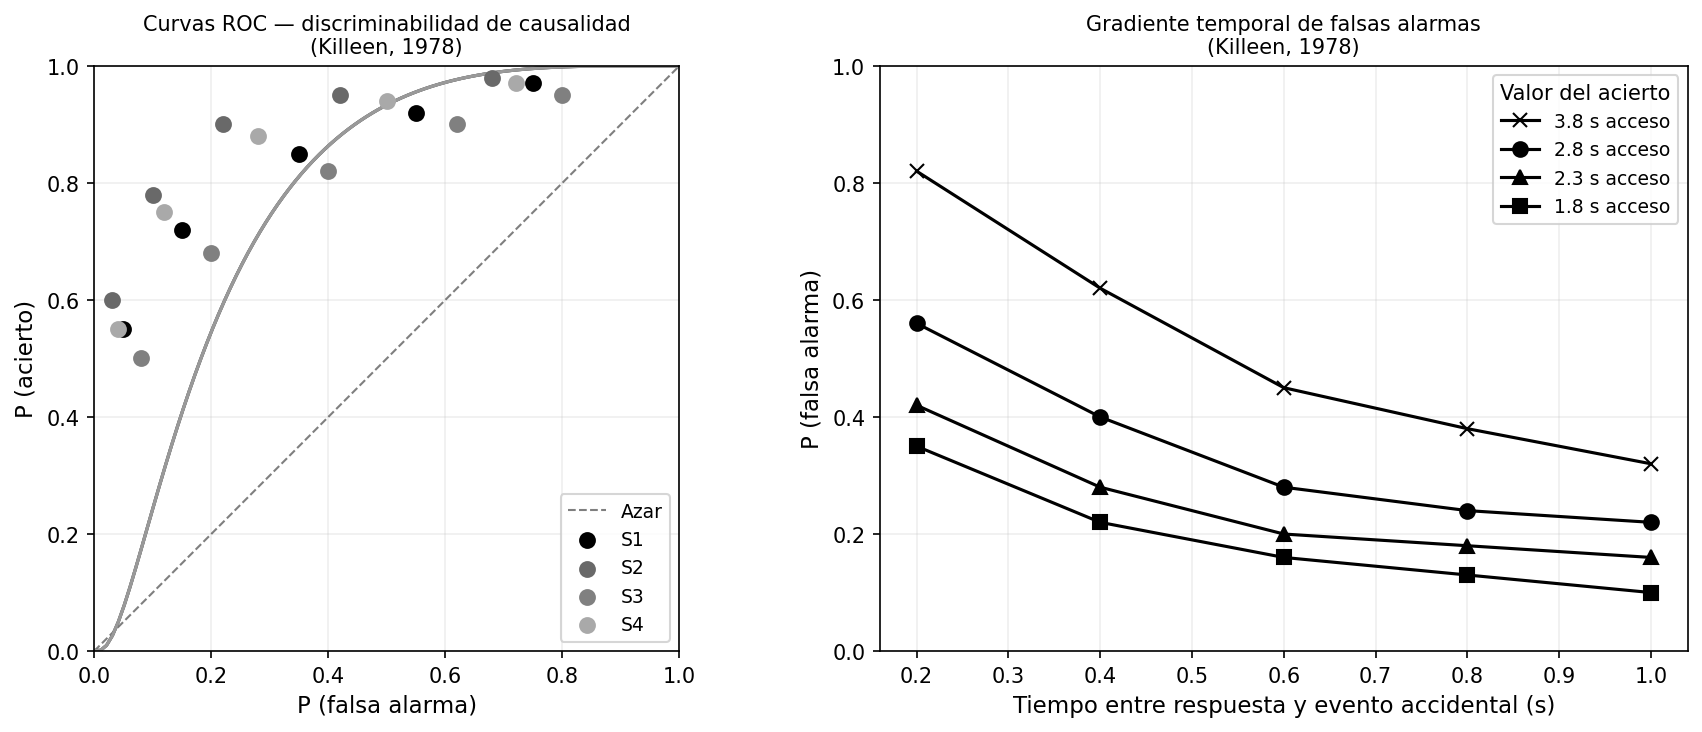
\includegraphics[width=7.8125in,height=\textheight,keepaspectratio]{Figuras/figura_9_4_5_killeen.png}

}

\caption{Resultados de Killen (1978)}

\end{figure}%

\begin{quote}
\textbf{Note}

\textbf{Descripción} Panel izzquierdo: Curvas ROC para cuatro palomas en
el experimento de Killeen (1978). Eje horizontal: P(falsa alarma). Eje
vertical: P(acierto). Línea punteada diagonal: rendimiento al azar. Las
curvas de los cuatro sujetos se ubican por encima de la diagonal; la
discriminabilidad fue de aproximadamente el 80\% en los ensayos. Cada
punto corresponde a una condición distinta de pago. Panel derecho: Eje
horizontal: tiempo entre la respuesta de la paloma y el evento no
contingente (0.2 a 1.0 segundos). Eje vertical: P(falsa alarma). Cuatro
curvas, una por condición de pago (1.8, 2.3, 2.8 y 3.8 segundos de
acceso a comida). En todas las condiciones, la probabilidad de falsa
alarma disminuye conforme aumenta la separación temporal. Datos de
Killeen (1978)
\end{quote}

El segundo resultado es que el criterio de decisión es flexible y
sensible a los pagos. Cuando los aciertos valían mucha comida, las
palomas adoptaban un criterio liberal: respondían con frecuencia que el
apagado había sido causado por ellas, lo que incrementaba tanto los
aciertos como las falsas alarmas. Cuando los aciertos valían poca
comida, el criterio se volvía conservador. Es exactamente lo que haría
un observador racional que maximiza la ganancia esperada: si detectar
causalidad cuando existe vale mucho y el costo de una falsa alarma es
bajo, conviene ser generoso en las atribuciones causales. Si acertar
vale poco o equivocarse es costoso, conviene ser conservador.

El tercer resultado es quizás el más revelador para la discusión sobre
contigüidad. Killeen también hizo algo que vale la pena que ustedes
ponderen antes de ver el resultado. Varió el tiempo transcurrido entre
la respuesta de la paloma y el apagado de luz \emph{no contingente}
---es decir, el tiempo entre la respuesta y el evento accidental
posterior. La probabilidad de falsa alarma disminuye sistemáticamente
conforme ese intervalo se alarga, desde 0.2 segundos hasta 1.0 segundos.
¿Por qué? Porque la contigüidad temporal opera como señal de posible
causalidad ---y a mayor distancia temporal, la señal se debilita. No es
un mecanismo determinístico; es un heurístico que disminuye con la
demora.

El cuadro que emerge de los tres experimentos ---Dickinson, Lattal y
Killeen--- es consistente. Los organismos son detectores de contingencia
estadística dotados de un sistema de decisión ajustable. Integran
información a lo largo de ventanas temporales amplias para estimar si
sus respuestas covarian con los SBIs. Utilizan la proximidad temporal
como heurístico ---y por eso son susceptibles a falsas alarmas cuando
eventos accidentales quedan cerca de sus respuestas. Y calibran su
criterio de decisión según los costos y beneficios de acertar y
equivocarse en cada contexto particular.

\section{Por qué la contigüidad es un buen sesgo, y cuándo
falla}\label{por-quuxe9-la-contiguxfcidad-es-un-buen-sesgo-y-cuuxe1ndo-falla}

Si los organismos son detectores de contingencia estadística más que
registradores de contigüidad, ¿por qué la contigüidad temporal funciona
tan bien como regla práctica en la mayoría de los entornos naturales?

La respuesta tiene que ver con la estructura causal del entorno
ancestral. La mayoría de los mecanismos causales biológicamente
relevantes ---un depredador que ataca, una fruta que cae, una trampa que
se cierra--- operan con rapidez. La demora entre una acción y sus
consecuencias en esos contextos es de segundos, no de horas. Cuando las
cadenas causales son cortas y los mecanismos rápidos, la contigüidad
temporal es un indicador confiable de causalidad real. La selección
natural favoreció sistemas que buscan primero en el vecindario temporal
inmediato de cada consecuencia inesperada, porque en ese vecindario se
encuentran la mayoría de las causas reales.

Pero el heurístico falla en condiciones específicas. Cuando las cadenas
causales son largas ---como en muchas relaciones entre comportamiento y
sus consecuencias en el entorno humano--- la acción y el resultado
pueden estar separados por horas o días. Cuando los SBIs son frecuentes
e independientes de la conducta del organismo ---como en entornos muy
enriquecidos con consecuencias no contingentes--- la tasa de
contigüidades accidentales sube y con ella la tasa de falsas alarmas. Y
cuando el organismo ejecuta muchas respuestas concurrentes, el problema
de asignar crédito a la respuesta correcta entre varias candidatas se
vuelve especialmente difícil.

En esas condiciones, la contigüidad como heurístico produce errores
sistemáticos ---los que se conocen coloquialmente como ``conductas
supersticiosas''. No son fallas del mecanismo; son la consecuencia
predecible de aplicar un heurístico adaptado a cierto tipo de entorno en
condiciones diferentes.

\section{Apertura hacia los modelos
formales}\label{apertura-hacia-los-modelos-formales}

Todo lo que hemos discutido en este capítulo puede reformularse con una
pregunta computacional precisa: ¿cómo actualiza un agente el valor que
asigna a un evento ---estímulo o respuesta--- en función de los
resultados que ha obtenido en el pasado? Esa pregunta tiene una
respuesta formal, y el siguiente capítulo la desarrolla a partir de la
ecuación que Bush y Mosteller propusieron a mediados del siglo XX. El
modelo es general: opera sobre cualquier evento predictivo, sea un
estímulo que anticipa un SBI o una respuesta que lo produce. Por eso cap
10 cierra al mismo tiempo los dos capítulos precedentes.

La idea central es sencilla: el valor que el agente asigna a un evento
se actualiza en cada ocasión, y la magnitud de esa actualización depende
de la discrepancia entre lo que ocurrió y lo que se esperaba. Si el
evento fue seguido de más SBI del anticipado, su valor sube; si fue
seguido de menos, baja. Lo que hace esta ecuación especialmente
interesante es que puede leerse de más de una manera: como un integrador
con fuga, como un proceso de reducción de error de predicción, y como un
filtro de media exponencial corrida que pondera más los eventos
recientes. Cada lectura ilumina un aspecto distinto del mecanismo. El
siguiente capítulo examina las tres con detalle.

\begin{center}\rule{0.5\linewidth}{0.5pt}\end{center}

\section{Simulador 7.1: Inducción temporal y respuestas
interinas/terminales}\label{simulador-7.1-inducciuxf3n-temporal-y-respuestas-interinasterminales}

El siguiente código implementa una versión simplificada de la dinámica
temporal que Staddon y Simmelhag documentaron. El SBI induce dos clases
de respuestas cuya probabilidad cambia a lo largo del intervalo entre
entregas: las interinas, que alcanzan su máximo poco después del SBI
anterior, y las terminales, que crecen conforme se acerca el siguiente
SBI.

\textbf{{[}SIMULADOR 7.1 --- Disponible en línea. El simulador
implementa la dinámica temporal de Staddon y Simmelhag: el SBI induce
respuestas interinas y terminales cuya probabilidad cambia a lo largo
del intervalo entre entregas. Parámetros ajustables: duración del
intervalo, tasa de decaimiento de las respuestas interinas, tasa de
crecimiento de las terminales, número de intervalos a simular.{]}}

\textbf{Ejercicios con el Simulador 7.1:}

\emph{Básico.} Con los parámetros predeterminados (intervalo de 15
segundos), observa en qué momento del intervalo las dos curvas se
cruzan. ¿Tiene sentido que Staddon y Simmelhag encontraran respuestas
interinas en la primera mitad del intervalo y terminales en la segunda
mitad?

\emph{Intermedio.} Cambia el intervalo a 30 segundos y luego a 5
segundos. ¿Cómo cambia la ventana temporal en que dominan las respuestas
interinas? ¿Qué predice esto sobre la distribución de respuestas cuando
el SBI ocurre muy frecuentemente?

\emph{Avanzado.} Modifica el parámetro \texttt{DECAIMIENTO} al mismo
valor que \texttt{ANTICIPACION}. ¿Qué forma toman las curvas?
¿Desaparecerían prácticamente las respuestas interinas si el decaimiento
fuera muy rápido? Relaciona tu respuesta con la idea de que las
respuestas interinas son ``conductas de espera'' que llenan el tiempo
entre SBIs.

\begin{center}\rule{0.5\linewidth}{0.5pt}\end{center}

\section{Simulador 7.2: Detección de contingencia con gradiente de
demora}\label{simulador-7.2-detecciuxf3n-de-contingencia-con-gradiente-de-demora}

Este simulador implementa un agente que aprende la tasa de SBIs
contingentes a su respuesta versus la tasa de SBIs no contingentes, con
un gradiente de demora que pondera más los SBIs cercanos en el tiempo.

\textbf{{[}SIMULADOR 7.2 --- Disponible en línea. El simulador
implementa un agente que aprende la tasa de SBIs contingentes a su
respuesta versus la tasa de SBIs no contingentes, con un gradiente de
demora exponencial. Parámetros ajustables: P(SBI \textbar{} respuesta),
P(SBI \textbar{} no respuesta), tasa de aprendizaje α, demoras a
comparar, número de sesiones.{]}}

\textbf{Ejercicios con el Simulador 7.2:}

\emph{Básico.} Observa cómo cambia la curva de aprendizaje al aumentar
la demora de 0 a 32 segundos. ¿A partir de qué demora el agente deja de
aprender claramente? Compara tu respuesta con los datos de Dickinson.

\emph{Intermedio.} Cambia \texttt{P\_SBI\_SIN\_RESPUESTA} al mismo valor
que \texttt{P\_SBI\_DADO\_RESPUESTA}. ¿Qué ocurre con el aprendizaje?
Explica por qué en términos de contingencia estadística: ¿qué cambia en
la relación entre respuesta y SBI?

\emph{Avanzado.} Modifica la función \texttt{simular\_aprendizaje} para
que el gradiente de demora sea lineal en lugar de exponencial. ¿Cambia
cualitativamente el patrón de resultados? ¿Qué forma del gradiente
parece más consistente con los datos de Dickinson?

\begin{center}\rule{0.5\linewidth}{0.5pt}\end{center}

\section{Conexiones}\label{conexiones-2}

\subsection{Hacia atrás: Asignación de crédito a estímulos (Capítulo
6)}\label{hacia-atruxe1s-asignaciuxf3n-de-cruxe9dito-a-estuxedmulos-capuxedtulo-6}

La estructura argumentativa de este capítulo replica la del anterior. En
el capítulo 8, la pregunta era si la contigüidad entre estímulo y SBI
era condición necesaria y suficiente para el aprendizaje predictivo; la
conclusión fue que no lo era en ninguna de las dos direcciones. Aquí la
misma pregunta se formula para las respuestas, y la conclusión es la
misma. El paralelismo no es casual: ambos problemas son instancias del
problema de la asignación de crédito, y ambos se resuelven con el mismo
mecanismo subyacente ---la detección de contingencia estadística,
modulada por sesgos inductivos que priorizan el espacio de búsqueda.

\subsection{Hacia adelante: La ecuación de Bush y Mosteller (Capítulo
8)}\label{hacia-adelante-la-ecuaciuxf3n-de-bush-y-mosteller-capuxedtulo-8}

El siguiente capítulo formaliza el mecanismo de actualización del valor
que este capítulo ha descrito en términos cualitativos. La ecuación de
Bush y Mosteller captura la idea central: el valor de una acción se
ajusta en proporción a la discrepancia entre lo que ocurrió y lo que se
esperaba. El lector que haya comprendido la lógica del aprendizaje por
contingencia en este capítulo estará en buena posición para apreciar por
qué esa ecuación tiene la forma que tiene ---y para examinar las
distintas maneras en que puede interpretarse.

\subsection{Lateral: Programas de refuerzo e igualación (Bloque
IV)}\label{lateral-programas-de-refuerzo-e-igualaciuxf3n-bloque-iv}

La distinción entre perspectiva molecular y perspectiva molar que
introdujimos brevemente en este capítulo se volverá central en el Bloque
IV. Los programas de refuerzo ---reglas que especifican qué respuestas
producen SBIs y con qué probabilidades--- producen patrones de
comportamiento que las teorías moleculares han tenido dificultades para
predecir. Las perspectivas molares de Baum y el modelo formal de Killeen
---que reservamos intencionalmente para ese bloque--- ofrecen
descripciones más precisas de esos patrones, y su presentación allí
tendrá más fuerza porque los estudiantes conocerán ya los datos que
intentan explicar.

\section{Ejercicios}\label{ejercicios-1}

\textbf{1.} El capítulo distingue entre el \emph{origen} del repertorio
conductual y la \emph{selección} entre ese repertorio. ¿Cuál de las dos
preguntas responde la Ley del Efecto? ¿Qué observación de los datos de
Thorndike plantea la pregunta que la Ley del Efecto no responde?

\textbf{2.} Staddon y Simmelhag encontraron que las respuestas
terminales eran más consistentes entre palomas que las respuestas
interinas, a pesar de que las terminales eran las que más frecuentemente
precedían a la comida. ¿Por qué este resultado contradice la explicación
de Skinner? ¿Qué predice el principio de inducción que se aplica aquí?

\textbf{3.} Describe con tus propias palabras el procedimiento de
Dickinson. ¿Cuál era el problema metodológico que el procedimiento
intentaba resolver? ¿Por qué era necesario el grupo yoked para
interpretar los resultados?

\textbf{4.} En el experimento de Lattal, las palomas aprendieron a picar
la tecla a pesar de que el procedimiento DRO garantizaba que la comida
nunca podía seguir inmediatamente a una respuesta. ¿Cómo interpretarías
este resultado desde la perspectiva molecular? ¿Y desde la perspectiva
molar? ¿Cuál de las dos interpretaciones parece más consistente con el
resultado?

\textbf{5.} En el experimento de Killeen, las palomas adoptaban un
criterio más liberal para atribuir causalidad cuando los aciertos valían
más comida. Traduce este resultado a un contexto cotidiano: ¿puedes
pensar en una situación humana en que el valor de acertar en una
atribución causal lleva a las personas a atribuir causalidad con más
frecuencia, incluso cuando la evidencia es ambigua? ¿Cuándo sería eso
adaptativo y cuándo podría ser problemático?

\textbf{6.} El capítulo argumenta que la contigüidad es un buen
heurístico en entornos donde los mecanismos causales operan rápido y las
cadenas causales son cortas. Describe dos contextos ---uno natural, uno
del entorno humano contemporáneo--- donde ese heurístico produce
inferencias causales correctas, y dos contextos donde produce errores
sistemáticos. ¿Qué tienen en común los contextos donde falla?

\textbf{7.} \emph{(Reflexión)} La conducta supersticiosa humana
---llevar amuletos, seguir rituales antes de un examen, evitar el número
trece--- puede interpretarse como resultado de los mismos mecanismos que
Killeen estudió en palomas. ¿Qué condiciones aumentarían la probabilidad
de que un organismo humano desarrolle una conducta supersticiosa? ¿Qué
condiciones la reducirían? ¿Qué dice este análisis sobre la racionalidad
de las supersticiones?

\section{Resumen}\label{resumen-3}

El problema adaptativo de este capítulo es el del control: aprender que
las propias acciones producen sucesos biológicamente importantes. Como
en el capítulo anterior con los estímulos, la pregunta central es si la
contigüidad temporal entre respuesta y SBI es condición necesaria y
suficiente para ese aprendizaje.

La respuesta es la misma: ni lo uno ni lo otro. No es suficiente porque
el experimento de Staddon y Simmelhag muestra que la contigüidad
accidental no puede dar cuenta del patrón organizado de respuestas
inducidas por el SBI; la organización temporal de ese patrón es
predecible desde el principio de inducción, no desde la contigüidad
accidental. No es necesaria porque Dickinson demostró que el aprendizaje
ocurre con demoras de hasta treinta y dos segundos ---y que ese
aprendizaje se debe a la relación de dependencia real, no a
contigüidades accidentales durante la demora--- y porque Lattal demostró
que el aprendizaje ocurre incluso cuando el procedimiento elimina por
diseño cualquier posibilidad de contigüidad.

Lo que los organismos detectan es covariación estadística: la tasa de
SBIs es mayor cuando la respuesta ocurre que cuando no ocurre. El
experimento de Killeen confirma que esa capacidad de detección es real y
funciona con alta precisión, que el criterio de decisión es ajustable
según los costos y beneficios de acertar y equivocarse, y que la
contigüidad temporal opera como señal de posible causalidad ---con el
resultado de que la probabilidad de atribuir causalidad a eventos
independientes decrece conforme aumenta la separación temporal.

El capítulo 10 formaliza el mecanismo de actualización que hace posible
esta detección de contingencia, a partir de la ecuación que Bush y
Mosteller propusieron para describir cómo el valor de una acción se
ajusta con la experiencia.

\section{Lecturas Recomendadas}\label{lecturas-recomendadas-1}

\textbf{Thorndike, E. L. (1911).} \emph{Animal Intelligence:
Experimental Studies.} Macmillan. --- El texto original de Thorndike,
con las observaciones sobre cajas puzzle que dieron origen a la Ley del
Efecto. Los capítulos centrales son accesibles y muestran el
razonamiento experimental de la época.

\textbf{Staddon, J. E. R., \& Simmelhag, V. L. (1971).} The
``superstition'' experiment: A reexamination of its implications for the
principles of adaptive behavior. \emph{Psychological Review, 78}, 3--43.
--- La réplica directa de Skinner, con datos detallados sobre la
distribución temporal de las respuestas. Más técnica, pero los
resultados hablan por sí mismos.

\textbf{Dickinson, A., Watt, A., \& Griffiths, W. J. H. (1992).}
Free-operant acquisition with delayed reinforcement. \emph{Quarterly
Journal of Experimental Psychology, 45B}, 241--258. --- El experimento
de demora con el diseño yoked. Nivel moderado; especialmente valiosa la
sección metodológica que justifica el uso del grupo de control.

\textbf{Lattal, K. A. (1987).} Considerations in the experimental
analysis of reinforcement delay. En M. L. Commons, J. E. Mazur, J. A.
Nevin \& H. Rachlin (Eds.), \emph{Quantitative Analyses of Behavior,
Vol. 5.} Erlbaum. --- El experimento DRO y su interpretación. Nivel
moderado.

\textbf{Killeen, P. R. (1978).} Superstition: A matter of bias, not
detectability. \emph{Science, 199}, 88--90. --- El experimento de
detección de causalidad en palomas. Tres páginas. Uno de los artículos
más elegantes de la literatura del aprendizaje.

\textbf{Timberlake, W., \& Lucas, G. A. (1989).} Behavior systems and
learning: From misbehavior to general principles. En S. B. Klein \& R.
R. Mowrer (Eds.), \emph{Contemporary Learning Theories.} Erlbaum. --- El
marco de sistemas de comportamiento aplicado al aprendizaje
instrumental. Conecta directamente con el capítulo 6 y da contexto para
el principio de inducción.

\begin{center}\rule{0.5\linewidth}{0.5pt}\end{center}

\bookmarksetup{startatroot}

\chapter{Aprendizaje por Refuerzo}\label{aprendizaje-por-refuerzo}

\section{El Modelo de Bush y
Mosteller}\label{el-modelo-de-bush-y-mosteller}

Los capítulos anteriores dejaron pendiente una promesa. En los capítulos
de kinesis y retroalimentación vimos mecanismos que permiten a los
organismos orientarse, navegar y regular variables internas con notable
eficiencia. Pero tienen una limitación que señalamos entonces: responden
a lo que ocurre \emph{ahora}, sin ninguna capacidad de anticipar lo que
está por ocurrir. El conductor que carga gasolina solo cuando el tanque
está vacío llegará varado tarde o temprano. Lo que le falta es la
capacidad de aprender que ciertas señales \emph{predicen} la necesidad
futura.

Los capítulos 6 y 7 establecieron las condiciones empíricas bajo las
cuales esa capacidad predictiva se desarrolla ---y las condiciones bajo
las cuales no se desarrolla. Mostraron que los organismos son detectores
de covariación estadística: aprenden que ciertos estímulos predicen
SBIs, y que ciertas respuestas los producen. Pero no describieron el
mecanismo formal que hace posible esa detección.

Este capítulo presenta ese mecanismo. En 1951, Robert Bush y Frederick
Mosteller propusieron una ecuación de actualización que ha demostrado
ser, pese a su simplicidad, una de las más productivas de la psicología
del siglo XX. La ecuación puede leerse de tres maneras distintas. Las
tres son algebraicamente idénticas, pero cada una ilumina un aspecto
diferente de lo que el mecanismo hace y por qué tiene la forma que
tiene.

Antes de la ecuación, sin embargo, conviene observar los datos que debe
explicar.

\section{Las curvas de aprendizaje}\label{las-curvas-de-aprendizaje}

Desde finales del siglo XIX, el estudio del aprendizaje ha producido una
regularidad empírica notable: cuando un organismo experimenta
repetidamente la relación entre un evento y un SBI, alguna medida de su
comportamiento cambia de forma característica. Aumenta rápidamente al
principio y se va estabilizando conforme el aprendizaje madura. La curva
resultante es negativamente acelerada ---ganancias grandes al inicio,
decrecientes con la práctica.

La figura 8.1 muestra un ejemplo con condicionamiento clásico: la
frecuencia del reflejo de parpadeo en humanos expuestos a un tono
seguido de un soplo al ojo, con diferentes intensidades del soplo
(Parssey, 1948). La figura 8.2 muestra un ejemplo instrumental: la
velocidad con que ratas tocan una palanca que produce comida, con
diferentes niveles de privación (Ramond, 1954). La forma de la curva es
la misma en ambos casos ---estímulo o respuesta, condicionamiento
clásico o instrumental, rata o humano. El modelo que presentamos en este
capítulo debe poder explicar ese patrón. Al final del capítulo veremos
por qué lo logra.

\begin{figure}[H]

{\centering 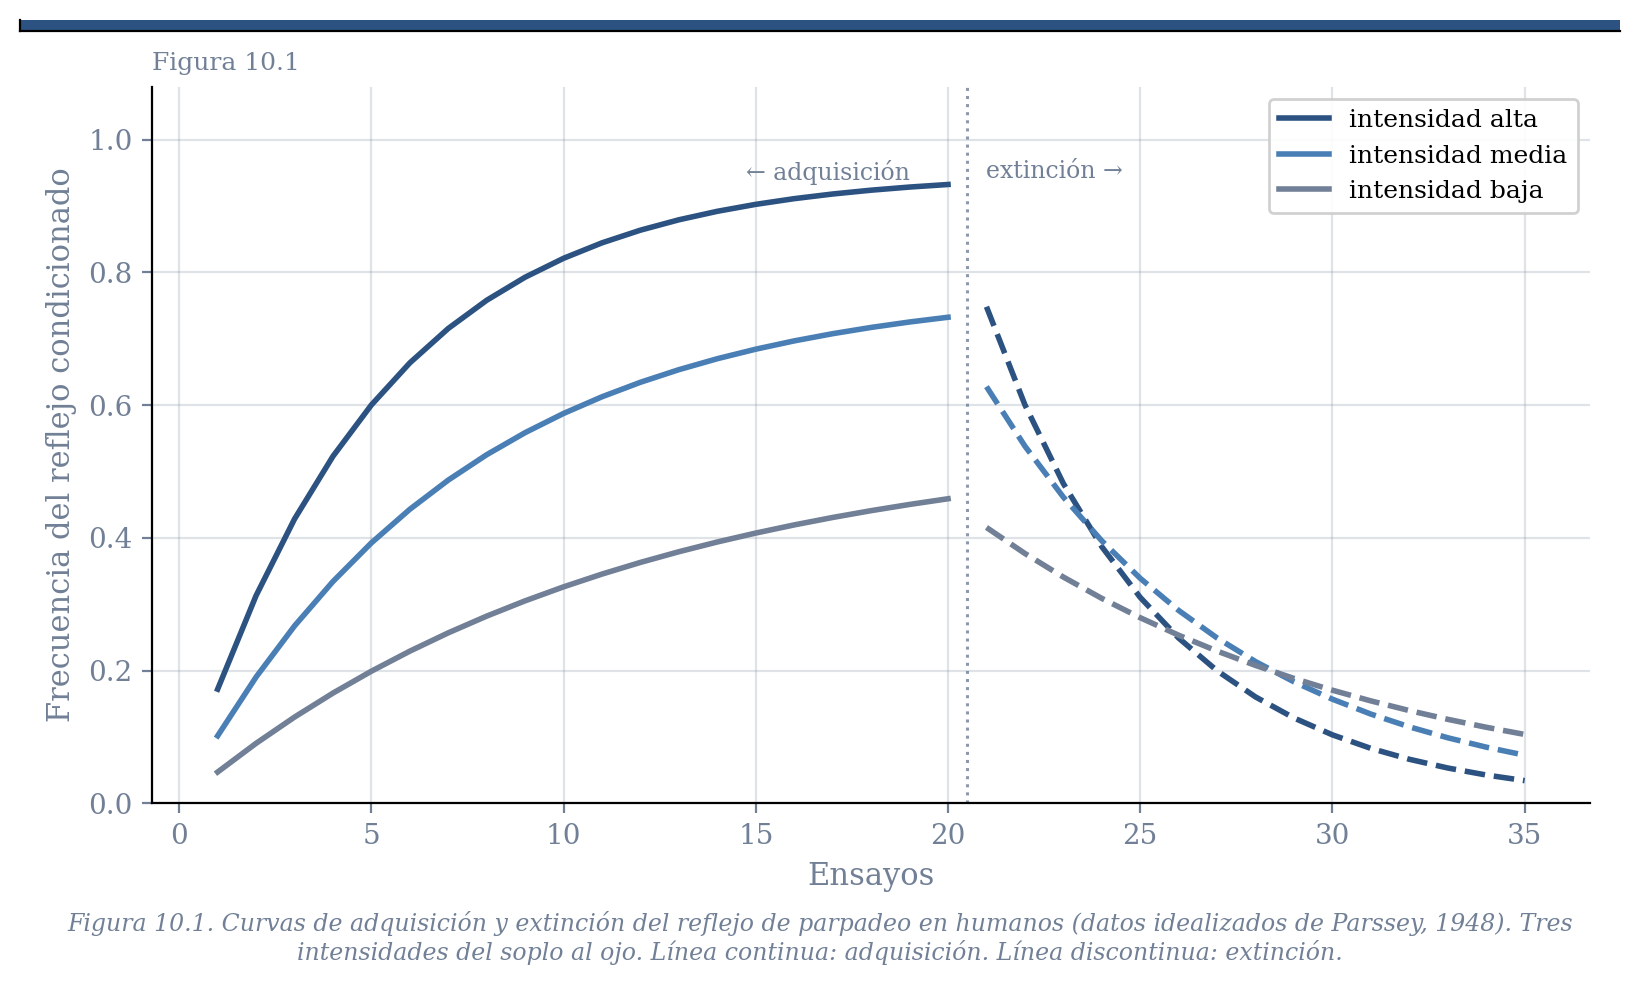
\includegraphics[width=7.8125in,height=\textheight,keepaspectratio]{Figuras/fig_10_1_parpadeo.png}

}

\caption{Curva de adquisición condicionamiento clásico}

\end{figure}%

\begin{quote}
\textbf{Note}

\textbf{Descripción}. Curvas de adquisición y extinción del reflejo de
parpadeo en humanos. Eje horizontal: ensayos. Eje vertical: frecuencia
del reflejo condicionado. Tres curvas para distintas intensidades del
soplo al ojo. Todas muestran el patrón negativamente acelerado durante
la adquisición y el declive durante la extinción. Datos de Parssey
(1948).{]}**
\end{quote}

\begin{figure}[H]

{\centering 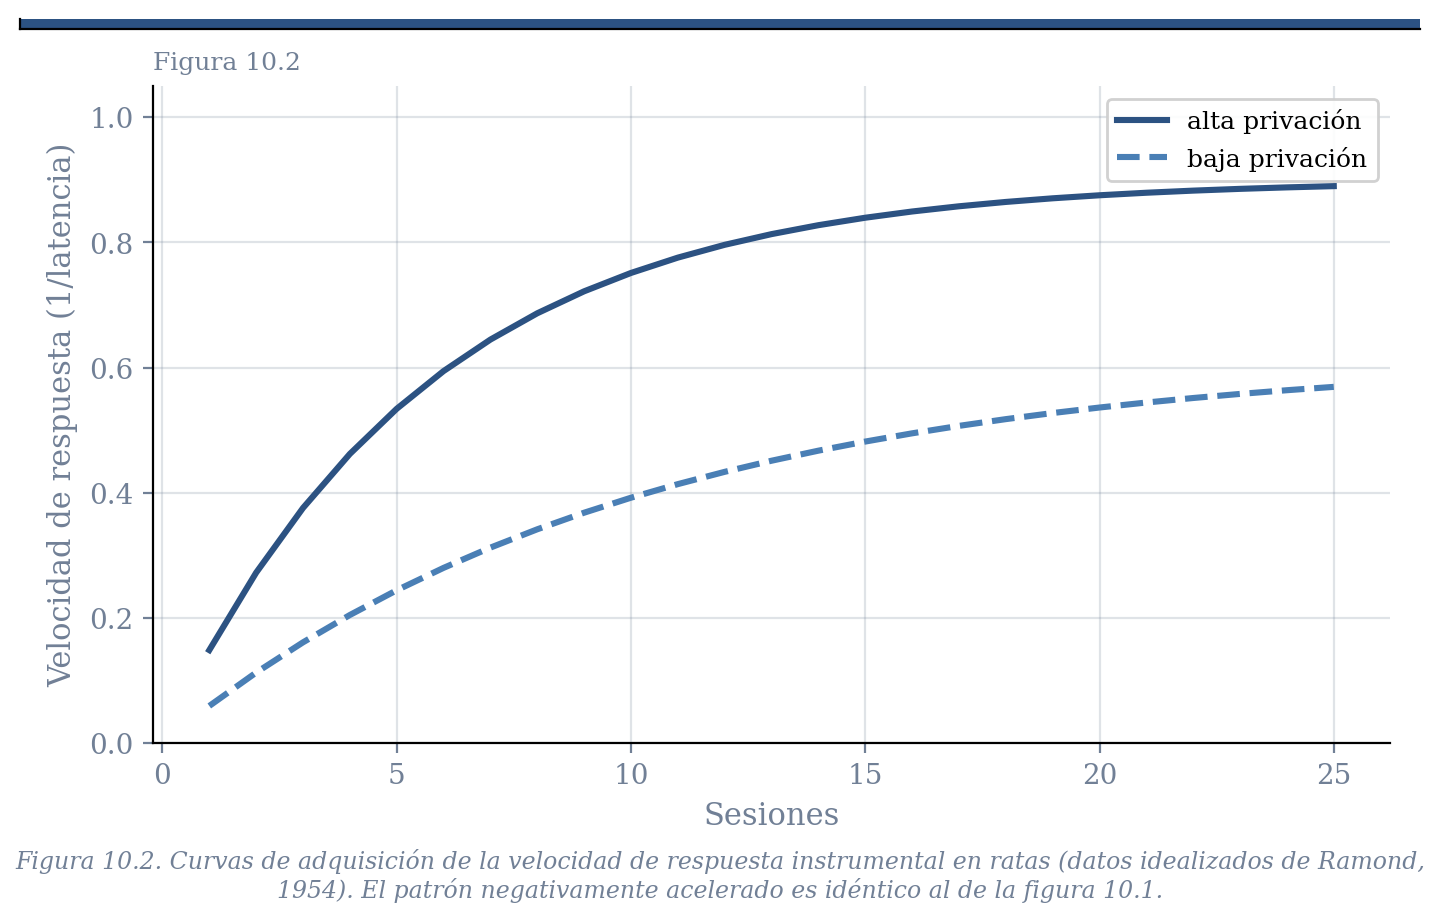
\includegraphics[width=7.8125in,height=\textheight,keepaspectratio]{Figuras/fig_10_2_velocidad.png}

}

\caption{fCurva de adquisición condicionamiento instrumental}

\end{figure}%

\begin{quote}
\textbf{Note}

\textbf{Descripción} Curva de adquisición de la velocidad de respuesta
en condicionamiento instrumental con ratas. Eje horizontal: sesiones.
Eje vertical: velocidad de respuesta. Dos curvas para dos niveles de
privación alimentaria. El patrón es cualitativamente idéntico al de la
figura 8.1. Datos de Ramond (1954).
\end{quote}

\begin{quote}
\textbf{Nota.} La curva negativamente acelerada es el patrón
\emph{promedio}, pero existe un debate sobre si refleja el aprendizaje
de organismos individuales o es un artefacto estadístico. Si distintos
organismos aprenden de manera abrupta ---un cambio discreto de no
responder a responder--- pero en ensayos distintos, el promedio grupal
producirá una curva continua aunque ningún individuo la siga. Skinner,
Estes y más recientemente Gallistel han insistido en analizar datos de
sujetos individuales por esta razón. En un capítulo posterior, cuando
examinemos los modelos de Gallistel sobre tiempo y correlaciones,
veremos que esa discusión tiene consecuencias formales sobre cómo debe
concebirse el mecanismo de aprendizaje.
\end{quote}

\section{Aprendizaje por Refuerzo: elementos
comunes}\label{aprendizaje-por-refuerzo-elementos-comunes}

Todos los modelos de aprendizaje por refuerzo comparten una arquitectura
básica. A cada evento que puede predecir un SBI ---sea un estímulo
condicionado o una respuesta--- se le asigna un número que representa su
\emph{valor predictivo} actual. A lo largo del siglo XX ese número
recibió distintos nombres: fuerza del reflejo, fuerza del hábito, fuerza
asociativa. Nosotros lo llamaremos valor predictivo ---\(V\) cuando
hablemos de estímulos, \(Q\) cuando hablemos de respuestas--- aunque en
lo que sigue usaremos \(V\) para los dos salvo donde la distinción
importe.

Una aclaración terminológica que conviene hacer desde el inicio: en la
literatura matemática del aprendizaje, al SBI se le llama
\emph{refuerzo} y se representa con \(R\) o con \(\lambda\). Usaremos
ese término en las ecuaciones y derivaciones que siguen, recordando que
es exactamente el mismo concepto que en los capítulos anteriores
llamamos suceso biológicamente importante. Refuerzo = SBI.

El modelo propone que \(V\) se actualiza en cada \emph{ensayo} ---cada
vez que el evento se presenta--- como función de lo que ocurre en ese
ensayo. Si el evento va seguido del refuerzo, \(V\) sube. Si ocurre sin
refuerzo, \(V\) baja. El mero paso del tiempo entre ensayos no cambia
\(V\); solo la experiencia directa con el evento lo modifica. Por eso se
dice que son modelos basados en ensayos.

El modelo es una instancia de un sistema de retroalimentación, como los
que vimos en el capítulo 5. La función del organismo transforma
refuerzos en valor predictivo. La función del entorno ---los programas
de refuerzo que estudiaremos en bloques posteriores--- transforma el
comportamiento en consecuencias. Las dos funciones están acopladas en un
lazo cerrado.

\section{Ecuaciones en diferencia: un lenguaje ya
conocido}\label{ecuaciones-en-diferencia-un-lenguaje-ya-conocido}

Antes de escribir la ecuación, conviene reconocer su forma. En capítulos
anteriores encontramos ecuaciones que describen cómo una variable cambia
de un momento al siguiente como función de su valor previo y de alguna
influencia externa. En el ejemplo de los contagios de covid, el número
de casos hoy dependía del número de casos ayer y de la tasa de
transmisión. En el modelo de ascenso de colina, el valor de la variable
de decisión en el siguiente instante dependía de su valor actual y del
cambio detectado en el entorno.

Esas ecuaciones se llaman \emph{ecuaciones en diferencia}: expresan el
estado del sistema en el tiempo \(t+1\) como función del estado en el
tiempo \(t\). Son ecuaciones recursivas que se aplican en cada paso al
resultado del paso anterior, y siempre requieren especificar un valor
inicial.

El modelo de Bush y Mosteller es exactamente una ecuación de esa
naturaleza. \(V_{t+1}\) ---el valor predictivo en el siguiente ensayo---
depende de \(V_t\) ---el valor acumulado hasta ahora--- y de \(R_t\)
---si hubo o no refuerzo en el ensayo actual. La dinámica que produce es
la misma clase de trayectoria que ya conocen: un sistema que evoluciona
ensayo a ensayo, que puede tener un equilibrio, y cuya trayectoria
depende de los parámetros y del valor inicial.

\section{Primera lectura: el integrador con
fuga}\label{primera-lectura-el-integrador-con-fuga}

La forma más directa de pensar en el modelo es como un proceso de carga
y descarga. Cada refuerzo \emph{carga} ---fortalece--- el valor del
evento, y cada presentación sin refuerzo lo \emph{descarga} ---lo
debilita. En este marco, \(V\) (o \(Q\)) es la cantidad de carga del
sistema en cada momento. La batería del teléfono es el análogo
cotidiano: se carga mientras está conectada, se descarga mientras se
usa, y en ningún momento llega a cero de golpe ni alcanza el máximo
instantáneamente.

Asumimos que \(V_{t+1}\) depende de solo dos factores: el valor
acumulado hasta ahora, \(V_t\), y lo que ocurrió en el ensayo actual,
\(R_t\) ---que vale 1 si hubo refuerzo y 0 si no lo hubo.

El punto clave es que estos dos factores no siempre deben tener el mismo
peso. En un entorno muy estable, donde la historia acumulada es un buen
predictor del futuro, tiene sentido darle más peso a la experiencia
pasada que al ensayo actual. En un entorno cambiante, donde el pasado
distante es poco relevante, tiene sentido darle más peso a la
experiencia reciente. El parámetro \(\alpha\) ---entre 0 y 1--- captura
exactamente esa importancia relativa: cuánto pesa la experiencia
acumulada frente al nuevo refuerzo. Si los dos factores deben sumar 1,
la ecuación queda:

\[V_{t+1} = (1-\alpha)\,V_t + \alpha\,R_t \qquad \text{donde } 0 < \alpha < 1\]

Esta es la ecuación del \emph{integrador con fuga}. El parámetro
\((1-\alpha)\) es el peso de la historia acumulada; \(\alpha\) es el
peso del refuerzo actual.

Para ver los dos procesos por separado, conviene examinar cada caso.
Cuando hay refuerzo (\(R_t = 1\)), la ecuación carga el sistema:
\(V_{t+1} = (1-\alpha)V_t + \alpha\), y el incremento es proporcional a
qué tan lejos está \(V\) de su máximo. Cuando no hay refuerzo
(\(R_t = 0\)), la ecuación se reduce a:

\[V_{t+1} = (1-\alpha)\,V_t\]

En este caso la descarga es pura: cada presentación del evento sin
refuerzo multiplica la carga actual por \((1-\alpha)\), reduciéndola en
una fracción \(\alpha\). Un sistema con mucha carga acumulada pierde más
en términos absolutos que uno con poca carga ---exactamente como una
batería que se descarga más rápido cuando está llena que cuando está
casi vacía.

Cuando \(\alpha\) es cercano a 0, la historia acumulada domina: cada
nuevo ensayo apenas mueve la cantidad de carga, y el sistema es
resistente a fluctuaciones pero lento para detectar cambios reales.
Cuando \(\alpha\) es cercano a 1, el refuerzo actual domina: el sistema
responde rápido a cambios pero es volátil ante fluctuaciones
accidentales. Pensemos en una amistad de muchos años que siempre ha sido
positiva. Una mañana esa persona no te saluda. Con \(\alpha\) cercano a
0, ese evento apenas altera tu valoración de la relación ---la historia
pesa más. Con \(\alpha\) cercano a 1, ese único evento tiene un peso
desproporcionado sobre años de experiencia acumulada. Ninguno de los dos
extremos es adaptativo en general; el valor óptimo de \(\alpha\) depende
de qué tan estable y predecible sea el entorno. Podemos ver que la
velocidad del aprendizaje depende del valor de \(\alpha\), y es así como
se le conoce en los libros de texto estandard.

La ecuación puede expresarse de dos formas equivalentes que la
literatura usa indistintamente. La primera enfatiza el \emph{nivel} del
valor predictivo ensayo a ensayo:

\[V_{t+1} = (1-\alpha)\,V_t + \alpha\,R_t\]

La segunda enfatiza el \emph{cambio} de ensayo a ensayo. Si definimos
\(\Delta V = V_{t+1} - V_t\), restando \(V_t\) de ambos lados:

\[\Delta V = \alpha\,(R_t - V_t)\]

Ambas formas son idénticas. La primera es útil para simular la
trayectoria de \(V\); la segunda hace visible de inmediato que el cambio
es proporcional a la discrepancia entre lo que ocurrió y lo que se
esperaba ---anticipando la segunda lectura.

Para ver cómo funciona la primera forma, sigamos el siguiente ejemplo
numérico. Con \(\alpha = 0.5\), \(V_0 = 0\), y cuatro ensayos de
adquisición seguidos de tres de extinción:

{\def\LTcaptype{none} % do not increment counter
\begin{longtable}[]{@{}
  >{\raggedright\arraybackslash}p{(\linewidth - 8\tabcolsep) * \real{0.1250}}
  >{\raggedright\arraybackslash}p{(\linewidth - 8\tabcolsep) * \real{0.1250}}
  >{\raggedright\arraybackslash}p{(\linewidth - 8\tabcolsep) * \real{0.1250}}
  >{\raggedright\arraybackslash}p{(\linewidth - 8\tabcolsep) * \real{0.5312}}
  >{\raggedright\arraybackslash}p{(\linewidth - 8\tabcolsep) * \real{0.0938}}@{}}
\toprule\noalign{}
\begin{minipage}[b]{\linewidth}\raggedright
Ensayo
\end{minipage} & \begin{minipage}[b]{\linewidth}\raggedright
\(R_t\)
\end{minipage} & \begin{minipage}[b]{\linewidth}\raggedright
\(V_t\)
\end{minipage} & \begin{minipage}[b]{\linewidth}\raggedright
\(V_{t+1} = 0.5\,V_t + 0.5\,R_t\)
\end{minipage} & \begin{minipage}[b]{\linewidth}\raggedright
Fase
\end{minipage} \\
\midrule\noalign{}
\endhead
\bottomrule\noalign{}
\endlastfoot
1 & 1 & 0.000 & 0.500 & Adquisición \\
2 & 1 & 0.500 & 0.750 & Adquisición \\
3 & 1 & 0.750 & 0.875 & Adquisición \\
4 & 1 & 0.875 & 0.938 & Adquisición \\
5 & 0 & 0.938 & 0.469 & Extinción \\
6 & 0 & 0.469 & 0.234 & Extinción \\
7 & 0 & 0.234 & 0.117 & Extinción \\
\end{longtable}
}

Noten el patrón en ambas fases. Durante la adquisición, el \(V\)
obtenido en cada ensayo se convierte en el nuevo \(V_t\) del ensayo
siguiente; el valor crece rápidamente al principio y se desacelera
conforme se aproxima a 1. Durante la extinción ---cuando \(R_t = 0\) y
la ecuación se reduce a \(V_{t+1} = (1-\alpha)V_t\)--- el proceso se
invierte: la carga disminuye en cada ensayo en una fracción \(\alpha\)
de su valor actual. Desde 0.938, la descarga es más rápida que desde
0.234, porque hay más carga que perder. Con \(\alpha = 0.2\) el proceso
de adquisición es más lento: \(V_1 = 0.2\), \(V_2 = 0.36\),
\(V_3 = 0.488\), \(V_4 = 0.590\); y la extinción también es más lenta.
La forma de las trayectorias es la misma; cambia la velocidad.

\begin{figure}[H]

{\centering 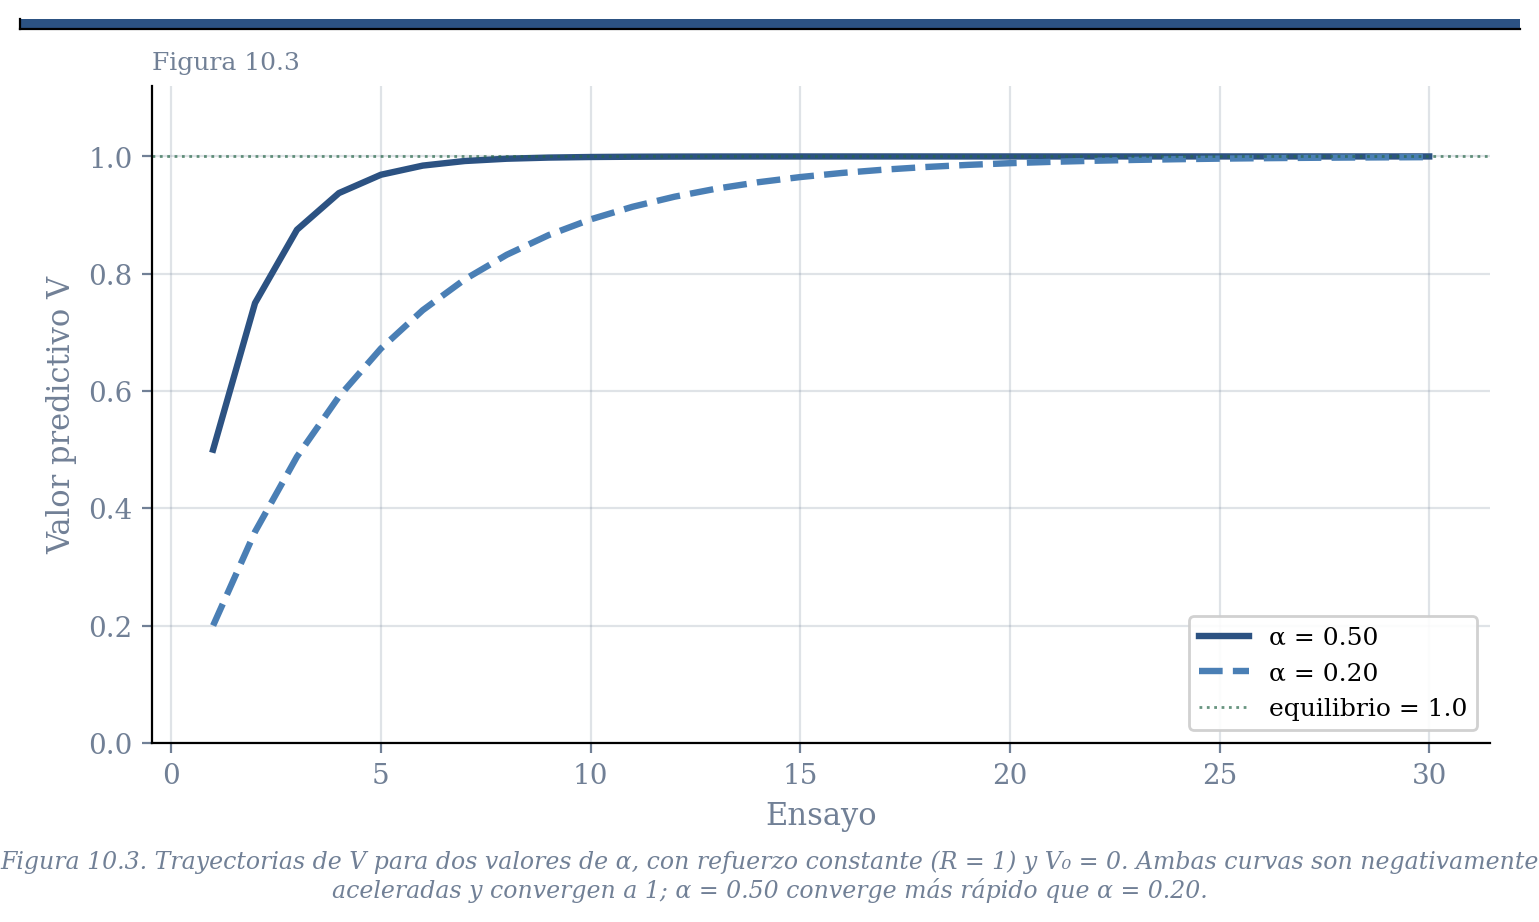
\includegraphics[width=7.8125in,height=\textheight,keepaspectratio]{Figuras/fig_10_3_trayectorias.png}

}

\caption{Curvas de aprendizaje para diferentes alphas}

\end{figure}%

\begin{quote}
\textbf{Note}

\textbf{Descripción}: Trayectorias de V para α = 0.2 y α = 0.5, con
refuerzo constante (R = 1) y V₀ = 0. Eje horizontal: ensayos. Eje
vertical: valor V. Ambas curvas son negativamente aceleradas y convergen
a 1, pero con velocidades distintas. Con α = 0.5 la convergencia es más
rápida; con α = 0.2 es más lenta y suave. Datos de las diapositivas del
curso.

\begin{figure}[H]

{\centering 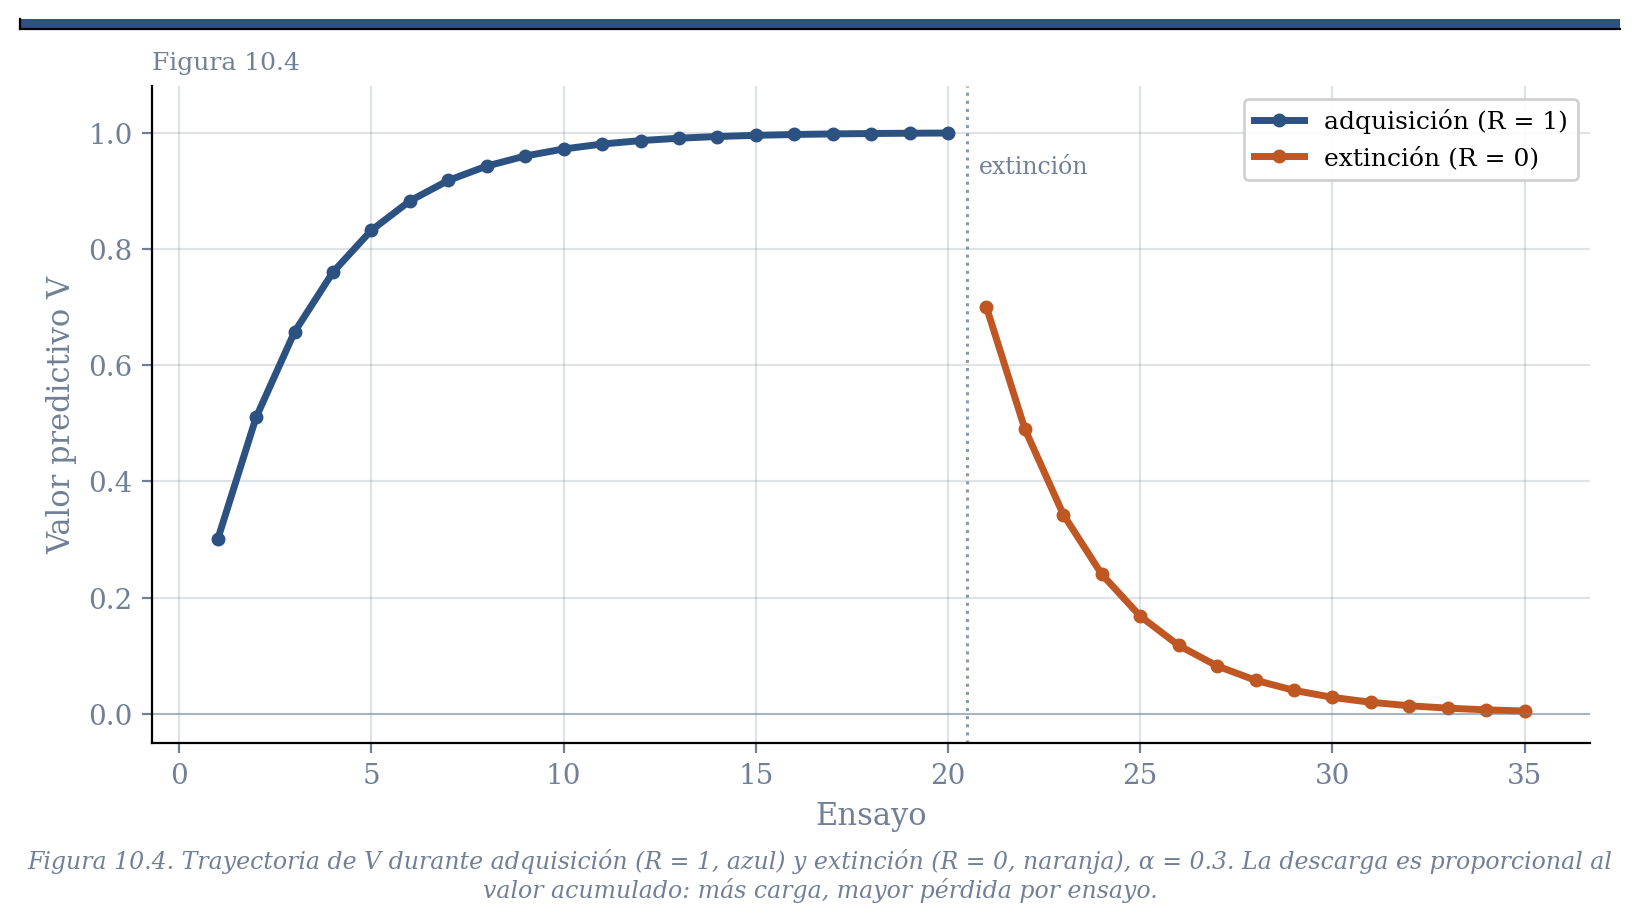
\includegraphics[width=7.8125in,height=\textheight,keepaspectratio]{Figuras/fig_10_4_adq_ext.png}

}

\caption{Trayectorias adquisición y extinción}

\end{figure}%

\begin{quote}
\textbf{Note}

\textbf{Descripción}: Trayectoria de V durante adquisición (R = 1) y
extinción (R = 0), α = 0.3. Eje horizontal: ensayos. Eje vertical: valor
V. V crece durante la adquisición siguiendo la curva negativamente
acelerada; decrece durante la extinción siguiendo una curva especular.
La tasa de cambio en ambas fases es proporcional al valor actual de V.

\mbox{}%
\section{Segunda lectura: la reducción del error de
predicción}\label{segunda-lectura-la-reducciuxf3n-del-error-de-predicciuxf3n}

La misma ecuación puede leerse de otra manera. Basta reordenar los
términos algebraicamente:

\[V_{t+1} = (1-\alpha)\,V_t + \alpha\,R_t\]

\[V_{t+1} = V_t - \alpha\,V_t + \alpha\,R_t\]

\[V_{t+1} = V_t + \alpha\,(R_t - V_t)\]

La expresión \((R_t - V_t)\) es la clave. Es la diferencia entre lo que
ocurrió (\(R_t\)) y lo que el organismo esperaba (\(V_t\)): el
\emph{error de predicción}. En la literatura contemporánea se representa
con \(\delta\):

\[\delta_t = R_t - V_t\]

Con esa notación, la ecuación del nivel queda:

\[V_{t+1} = V_t + \alpha\,\delta_t\]

Y la ecuación del cambio queda:

\[\Delta V = \alpha\,\delta_t\]

Si el refuerzo fue mayor de lo anticipado, \(\delta\) es positivo y
\(V\) sube. Si fue menor, \(\delta\) es negativo y \(V\) baja. Si el
refuerzo ocurrió exactamente como se esperaba ---\(R_t = V_t\)---
entonces \(\delta = 0\) y \(V\) no cambia. En la literatura
contemporánea, esta forma se conoce como la \emph{regla delta}, y es la
versión dominante en la psicología del aprendizaje y las neurociencias.

Esta lectura sugiere una intuición sobre el bloqueo de Kamin que vimos
en el capítulo 6. Si un estímulo ya predice perfectamente el refuerzo
---\(V_t = R_t\)--- entonces \(\delta_t = 0\): no hay sorpresa y no hay
nada que aprender. Cuando se presenta el compuesto AB, si A ya predice
el refuerzo perfectamente, el error de predicción debería ser cero y B
no debería aprender nada. La intuición es correcta, pero la ecuación de
Bush y Mosteller no puede derivarla formalmente: opera sobre eventos
individuales y no tiene mecanismo para distribuir el error de predicción
entre estímulos simultáneos. Esa extensión es precisamente lo que
Rescorla y Wagner añadieron en 1972, y es el tema del capítulo
siguiente.

La figura 8.5 muestra la evolución paralela de \(V\) y \(\delta\) a lo
largo del aprendizaje. Al inicio, cuando \(V\) es bajo y el refuerzo
ocurre, \(\delta\) es grande y positivo ---mucha sorpresa, mucho
aprendizaje. Conforme \(V\) crece y se aproxima al valor de equilibrio,
\(\delta\) se hace cada vez más pequeño. El aprendizaje se desacelera no
porque el mecanismo cambie, sino porque hay menos error que corregir. La
curva negativamente acelerada es, desde esta perspectiva, la
consecuencia directa de un sistema que aprende proporcionalmente a su
propia ignorancia.

\begin{figure}[H]

{\centering 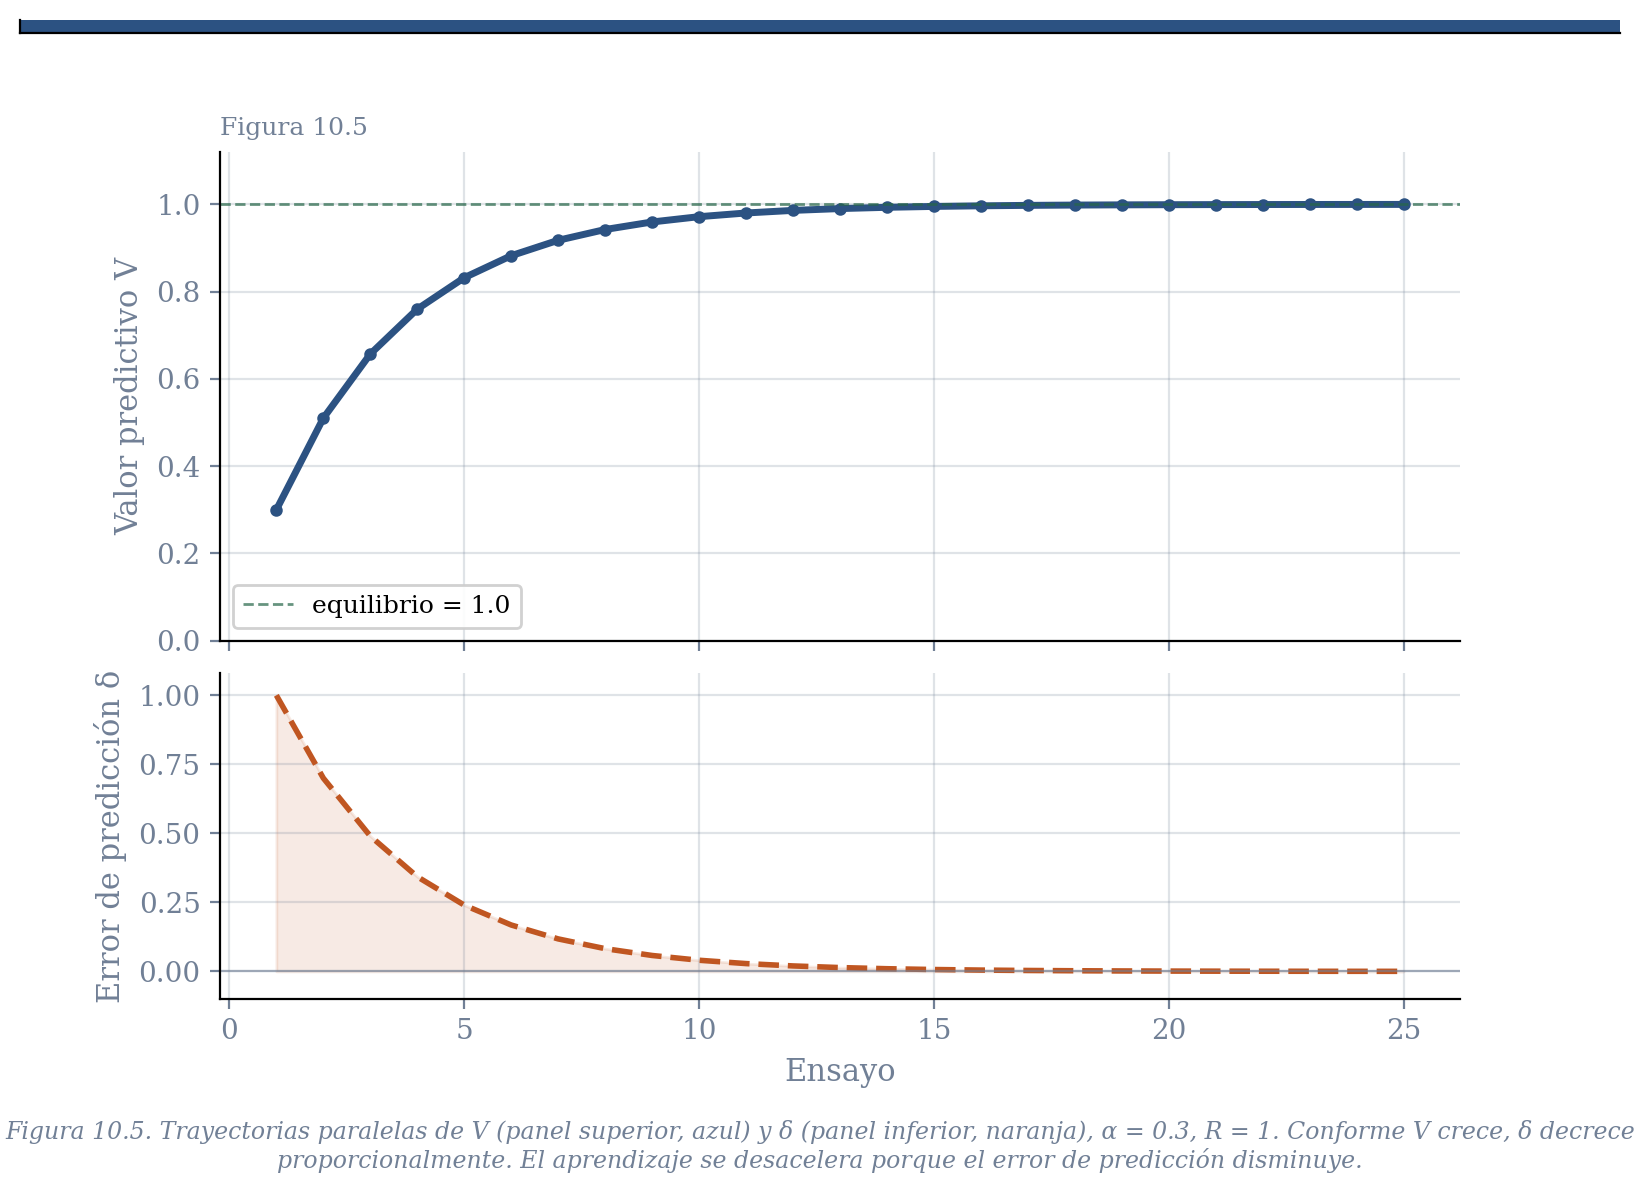
\includegraphics[width=7.8125in,height=\textheight,keepaspectratio]{Figuras/fig_10_5_V_delta.png}

}

\caption{Trayectoria de V y de error de predicción}

\end{figure}%

\begin{quote}
\textbf{Note}

\textbf{Descripción}: Trayectorias paralelas de V y δ. Panel superior: V
crece de 0 hacia 1 siguiendo la curva negativamente acelerada. Panel
inferior: δ decrece desde su valor máximo inicial hacia cero. La
relación entre las dos curvas ilustra que el aprendizaje se desacelera
porque el error de predicción disminuye. α = 0.3, R = 1.
\end{quote}

Esta lectura también conecta con la neurociencia. A finales de los años
noventa, Wolfram Schultz encontró que las neuronas dopaminérgicas del
mesencéfalo de primates se comportan exactamente como predice la señal
\(\delta\). Al inicio del entrenamiento disparan cuando ocurre el
refuerzo inesperado. Conforme el animal aprende, la respuesta
dopaminérgica se desplaza hacia el estímulo predictor ---el momento
donde se produce el error de predicción--- y desaparece en el momento
del refuerzo, porque este ya no es sorprendente. Cuando el refuerzo
esperado no ocurre, las neuronas muestran una supresión de actividad: un
error de predicción negativo. La dopamina no es simplemente una señal de
placer; es una señal de error de predicción.

\mbox{}%
\section{Tercera lectura: el filtro de media exponencial
corrida}\label{tercera-lectura-el-filtro-de-media-exponencial-corrida}

Hay una tercera forma de llegar a la misma ecuación. Es la que más
claramente revela qué está haciendo el organismo desde el punto de vista
estadístico, y es la que favoreceremos en capítulos posteriores cuando
examinemos entornos cambiantes.

El problema que enfrenta el organismo es, en el fondo, un problema de
estimación: dado todo lo que he observado hasta ahora, ¿cuál es la tasa
de refuerzo asociada a este evento? Para entender cómo el modelo
resuelve ese problema, conviene empezar con una estrategia más simple y
mostrar por qué no es suficiente.

\mbox{}%
\subsection{Medianas corridas y el problema del
alisamiento}\label{medianas-corridas-y-el-problema-del-alisamiento}

El problema que enfrenta el organismo es un problema de estimación: dado
todo lo que he observado, ¿cuál es la tasa de refuerzo asociada a este
evento? La estrategia más directa es calcular el promedio de todos los
refuerzos desde el primer ensayo:

\[V_t = \frac{1}{t}\sum_{i=1}^{t} R_i\]

Pero este promedio simple tiene dos limitaciones. Asigna el mismo peso a
todos los ensayos ---una observación de hace cien ensayos pesa igual que
la de ayer--- y no filtra el ruido de las fluctuaciones accidentales.

Para entender el problema del ruido y cómo resolverlo, consideremos el
ejemplo de los contagios diarios de covid, que ya conocen. Usamos la
\emph{mediana corrida} porque es fácil de calcular a mano y robusta ante
valores aberrantes; el argumento sobre alisamiento aplica igualmente a
la media. Se selecciona una ventana de cierto número de observaciones,
se calcula su mediana ---el valor central al ordenarlos--- y se desplaza
la ventana un paso a la derecha, repitiendo la operación.

Con los siguientes contagios diarios (en miles): 10, 14, 11, 16, 13, 9,
\textbf{85}, 12, 18, 15, 20, 17, 13, 19, 16, una mediana corrida de 3
produce: 11, 13, 13, 13, 11, 12, 15, 15, 18, 17, 17, 16, 16. El valor
aberrante de 85 desaparece, absorbido por sus vecinos, y la tendencia
ascendente queda visible. Una ventana de 5 suaviza más aún: 13, 13, 12,
13, 13, 15, 17, 17, 17, 17, 16.

\pandocbounded{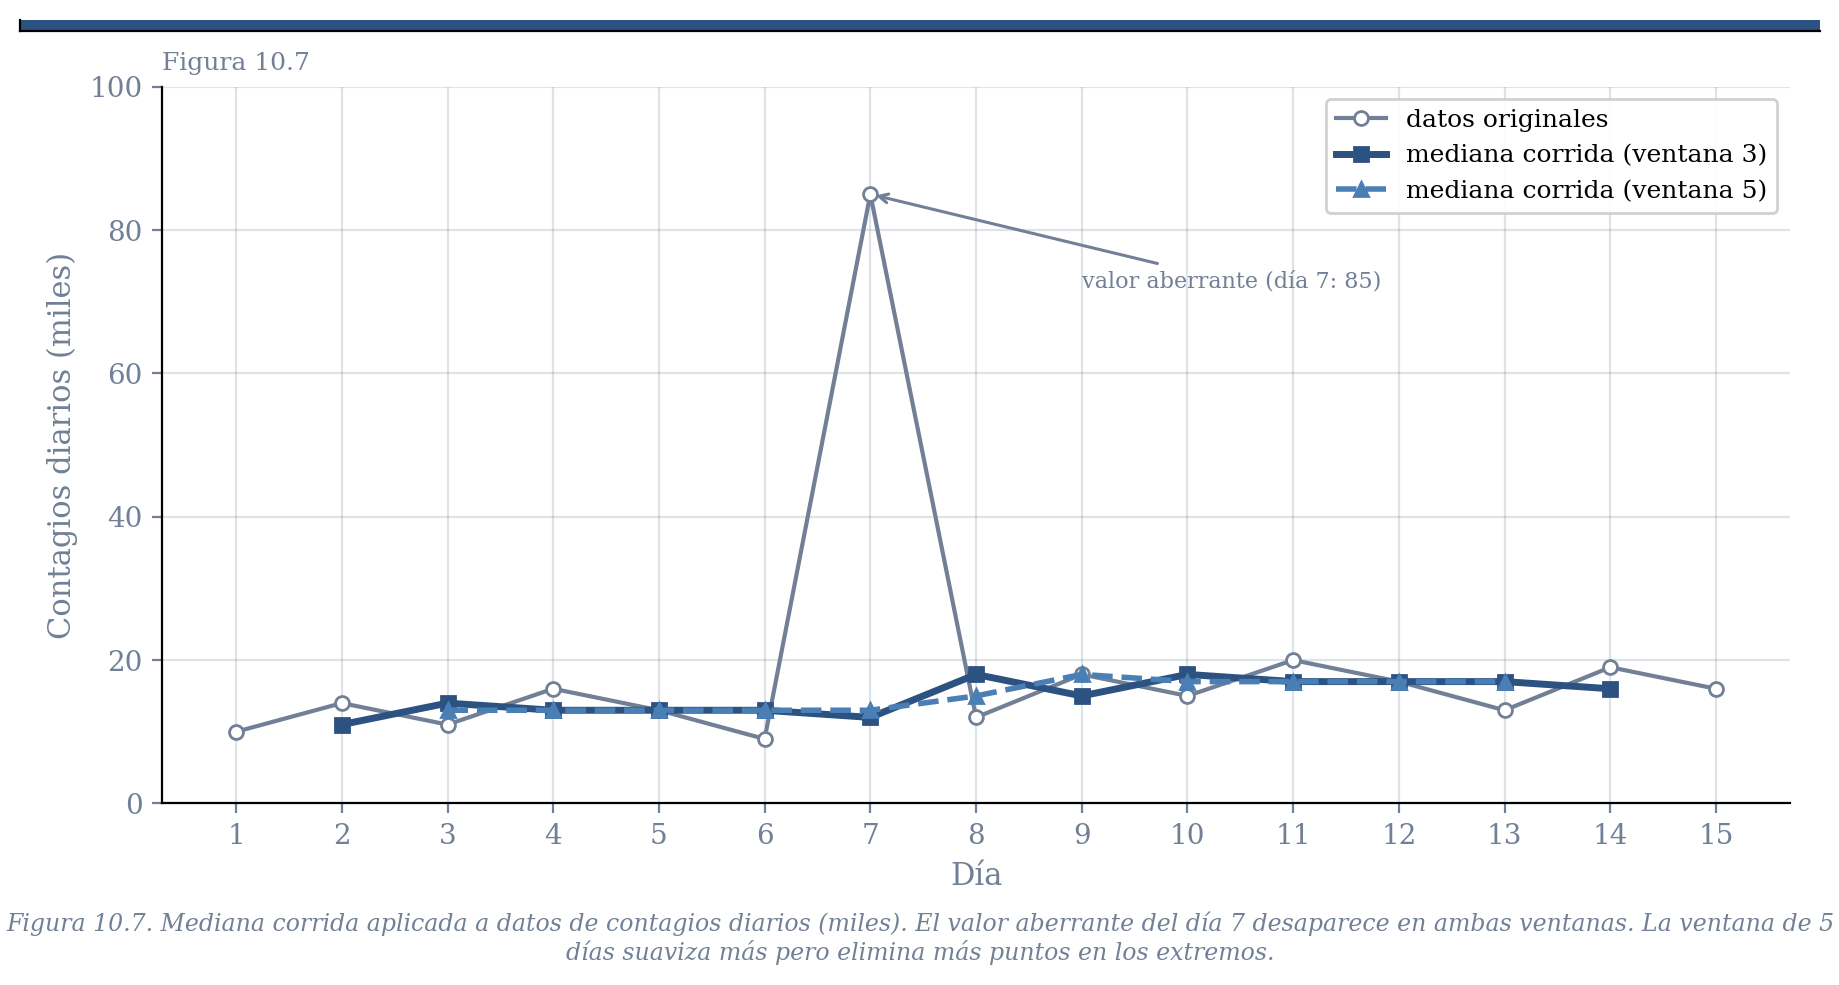
\includegraphics[keepaspectratio,alt={Mediana corrida}]{Figuras/fig_10_7_mediana_corrida.png}}\{\#figura\_10\_7\_mediana
corrida width=750 fig-align=``center''\}

\begin{quote}
\textbf{Note}

\textbf{Descripción}: Ejemplo de mediana corrida. Eje horizontal: días
(1--15). Eje vertical: contagios diarios (miles). Línea negra irregular:
datos originales, con el valor aberrante de 85 visible en el día 7.
Línea azul oscura: mediana corrida de ventana 3. Línea azul clara:
mediana corrida de ventana 5. Las dos ventanas eliminan el valor
aberrante y hacen visible la tendencia ascendente.
\end{quote}

La mediana corrida resuelve el ruido pero no el problema de los pesos
iguales: los datos de la primera semana pesan igual que los de ayer. Y
además es costosa: requiere almacenar toda la ventana en cada paso. En
la mayoría de los contextos adaptativos, tiene más sentido dar mayor
peso a las experiencias recientes.

\mbox{}%
\subsection{De la media simple a la regla
delta}\label{de-la-media-simple-a-la-regla-delta}

Para ver cómo la media simple se convierte en filtro exponencial,
conviene partir de un caso concreto. Consideremos una secuencia de
resultados de una máquina tragamonedas ---cada respuesta produce
refuerzo (1) o no (0) con cierta probabilidad constante:

\[1\;1\;0\;0\;0\;1\;0\;0\;1\;1\;1\;0\;0\;0\;1\;1\;0\;0\;1\;1\;0\;1\;0\;0\;1\;1\;1\;1\]

Para predecir el siguiente resultado, la estrategia más directa es
calcular la media de todos los resultados obtenidos hasta el ensayo
\(t\):

\[V_t = \frac{1}{t}\sum_{i=1}^{t} R_i\]

Pero esta fórmula exige recordar cada resultado desde el inicio y
sumarlos de nuevo en cada ensayo. Existe una forma equivalente que evita
ese costo. Partimos de la media en \(t\) y la media en \(t-1\):

\[V_t = \frac{1}{t}\sum_{i=1}^{t} R_i \qquad \qquad V_{t-1} = \frac{1}{t-1}\sum_{i=1}^{t-1} R_i\]

Expandemos las dos ecuaciones:

\[V_t = \frac{1}{t}\bigl(R_1 + R_2 + \cdots + R_{t-1} + R_t\bigr)\]

\[V_{t -1}= \frac{1}{t-1|}\bigl(R_1 + R_2 + \cdots + R_{t-1} )\]

Las dos ecuaciones comparten los términos \(R_1\) hasta \(R_{t-1}\).
Multiplicando la segunda por \((t-1)\) obtenemos justo esa suma
compartida:

\[(t-1)\,V_{t-1} = R_1 + R_2 + \cdots + R_{t-1}\]

Sustituyendo en la primera:

\[V_t = \frac{1}{t}\bigl((t-1)\,V_{t-1} + R_t\bigr)\]

Expandiendo y reordenando:

\[V_t = V_{t-1} + \frac{1}{t}\,(R_t - V_{t-1})\]

Esta es la media simple escrita como regla de actualización: para
calcular el nuevo promedio solo necesito el promedio anterior
\(V_{t-1}\) y el refuerzo actual \(R_t\). No hace falta almacenar ningún
resultado individual.

La forma de la ecuación debería resultar familiar: es la regla delta,
con el peso \(\frac{1}{t}\) en lugar de \(\alpha\). Pero ese peso tiene
un problema: decrece con cada ensayo nuevo. En el ensayo 10, cada
resultado pesa \(\frac{1}{10}\). En el ensayo 100, pesa
\(\frac{1}{100}\). Conforme se acumula experiencia, cada nueva
observación importa cada vez menos ---exactamente lo opuesto de lo que
queremos si el entorno puede cambiar.

\mbox{}%
\subsection{Del peso decreciente al peso
constante}\label{del-peso-decreciente-al-peso-constante}

La solución es directa: reemplazar el peso decreciente \(\frac{1}{t}\)
por un peso \emph{constante} \(\alpha\):

\[V_t = V_{t-1} + \alpha\,(R_t - V_{t-1})\]

Que es exactamente la regla delta. Con \(\alpha\) constante, cada nuevo
refuerzo siempre tiene el mismo peso relativo, sin importar cuántos
ensayos hayan transcurrido.

Pero ¿qué implica esto para los refuerzos del pasado? Para verlo,
conviene reescribir la ecuación en la forma del integrador:

\[V_t = (1-\alpha)\,V_{t-1} + \alpha\,R_t\]

Y ahora expandir \(V_{t-1}\) usando su propia ecuación, luego
\(V_{t-2}\), y así sucesivamente. La tabla siguiente muestra los
primeros tres pasos de la sustitución con \(V_0 = 0\):

{\def\LTcaptype{none} % do not increment counter
\begin{longtable}[]{@{}
  >{\raggedright\arraybackslash}p{(\linewidth - 4\tabcolsep) * \real{0.2000}}
  >{\raggedright\arraybackslash}p{(\linewidth - 4\tabcolsep) * \real{0.4333}}
  >{\raggedright\arraybackslash}p{(\linewidth - 4\tabcolsep) * \real{0.3667}}@{}}
\toprule\noalign{}
\begin{minipage}[b]{\linewidth}\raggedright
Paso
\end{minipage} & \begin{minipage}[b]{\linewidth}\raggedright
Sustitución
\end{minipage} & \begin{minipage}[b]{\linewidth}\raggedright
Resultado
\end{minipage} \\
\midrule\noalign{}
\endhead
\bottomrule\noalign{}
\endlastfoot
\(V_t\) & --- & \(\alpha R_t + (1-\alpha)V_{t-1}\) \\
Sustituyo \(V_{t-1}\) & \(V_{t-1} = \alpha R_{t-1} + (1-\alpha)V_{t-2}\)
& \(\alpha R_t + \alpha(1-\alpha)R_{t-1} + (1-\alpha)^2 V_{t-2}\) \\
Sustituyo \(V_{t-2}\) & \(V_{t-2} = \alpha R_{t-2} + (1-\alpha)V_{t-3}\)
&
\(\alpha R_t + \alpha(1-\alpha)R_{t-1} + \alpha(1-\alpha)^2 R_{t-2} + (1-\alpha)^3 V_{t-3}\) \\
Continúo hasta \(V_0 = 0\) & --- &
\(\alpha R_t + \alpha(1-\alpha)R_{t-1} + \alpha(1-\alpha)^2 R_{t-2} + \cdots + \alpha(1-\alpha)^{t-1}R_1\) \\
\end{longtable}
}

El patrón es claro: cada refuerzo pasado recibe un peso de la forma
\(\alpha(1-\alpha)^k\), donde \(k\) es el número de ensayos que lo
separan del presente. La fórmula general es entonces:

\[V_t = \alpha\,R_t + \alpha(1-\alpha)\,R_{t-1} + \alpha(1-\alpha)^2\,R_{t-2} + \cdots + \alpha(1-\alpha)^{t-1}\,R_1\]

El refuerzo más reciente \(R_t\) tiene peso \(\alpha\). El del ensayo
anterior tiene peso \(\alpha(1-\alpha)\). El de hace dos ensayos tiene
peso \(\alpha(1-\alpha)^2\). Los pesos decrecen exponencialmente hacia
el pasado ---de ahí el nombre: \emph{filtro de media exponencial
corrida}.

\begin{figure}[H]

{\centering 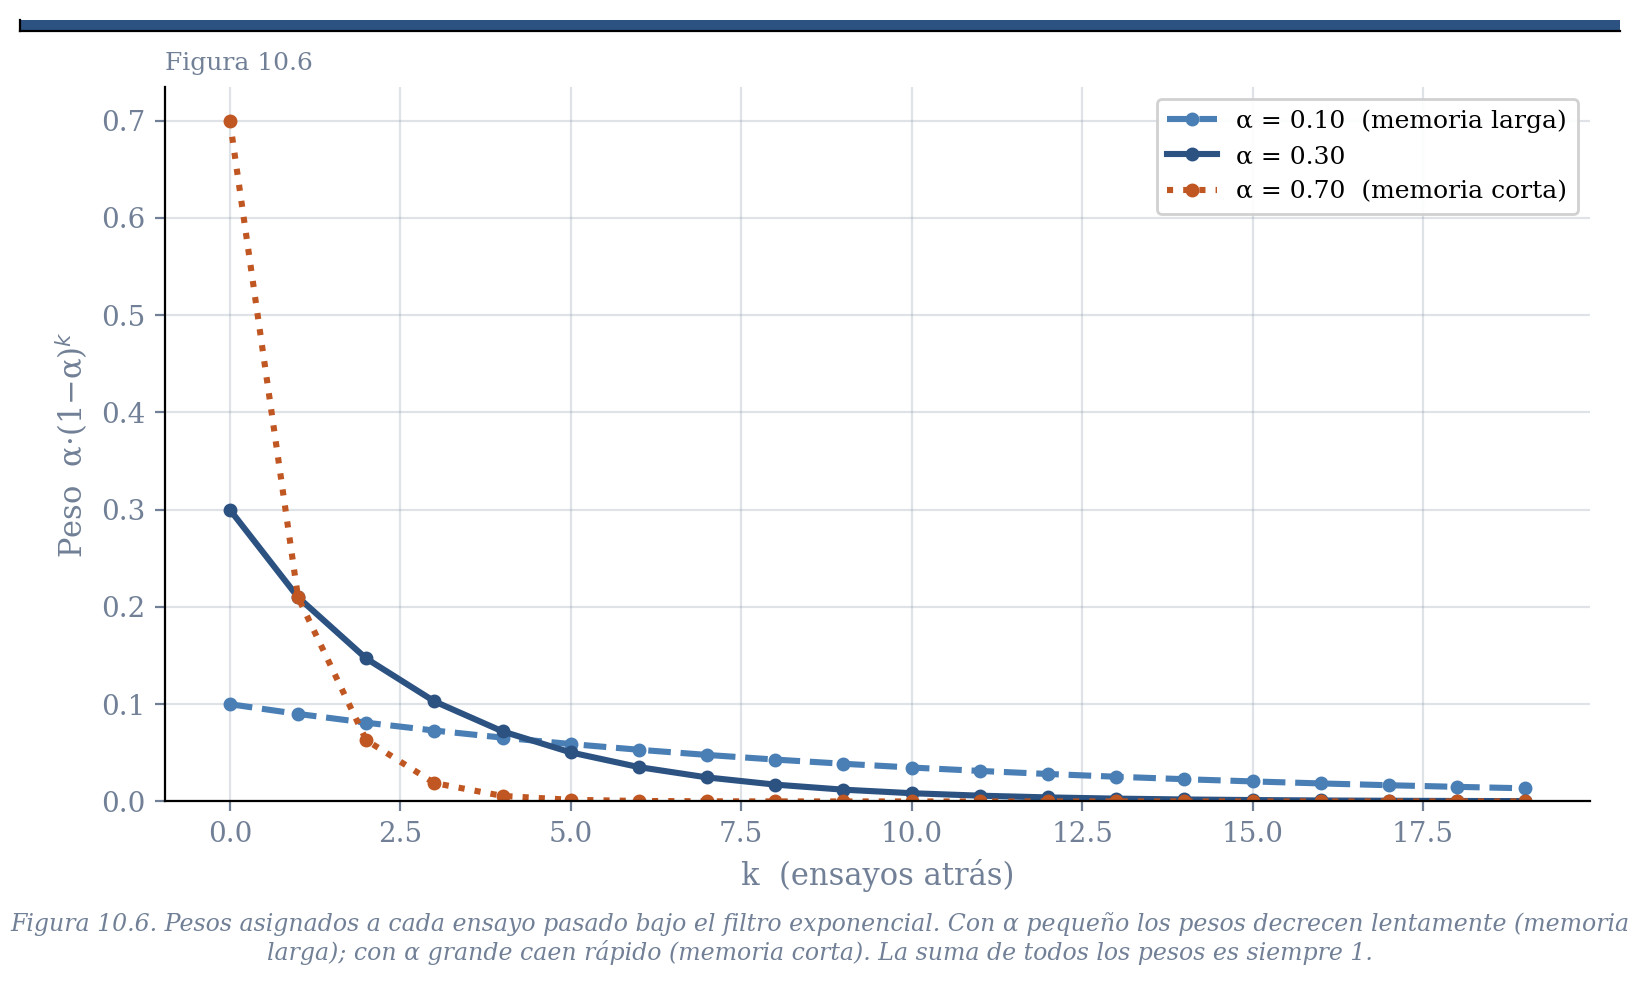
\includegraphics[width=7.8125in,height=\textheight,keepaspectratio]{Figuras/fig_10_6_pesos_exp.png}

}

\caption{Pesos de filtros exponenciales}

\end{figure}%

\begin{quote}
\textbf{Note}

\textbf{Descripción}: Pesos asignados a cada ensayo pasado bajo el
filtro exponencial, para α = 0.1, 0.3 y 0.7. Eje horizontal: distancia
temporal al pasado (ensayos). Eje vertical: peso de ponderación. Con α
pequeño, los pesos decrecen lentamente --- el organismo tiene memoria
larga. Con α grande, los pesos caen rápido --- el organismo tiene
memoria corta. En todos los casos, la suma de todos los pesos es 1.
\end{quote}

Esta tercera lectura revela lo que las otras dos no hacen tan explícito:
el organismo no registra eventos individuales. Estima un \emph{promedio
ponderado} de su historia de refuerzos, donde los más recientes pesan
más y el peso de cada observación decrece conforme queda más atrás en el
tiempo. El parámetro \(\alpha\) determina el tamaño efectivo de esa
ventana temporal: un \(\alpha\) pequeño equivale a una ventana larga
---memoria larga, resistente al ruido, lenta para detectar cambios
reales; un \(\alpha\) grande equivale a una ventana corta ---memoria
corta, sensible a cambios, pero también a fluctuaciones accidentales.

\begin{quote}
\textbf{🕹️ ¡Prueba el Simulador Interactivo!}

\href{https://colab.research.google.com/github/arbouria/Libro-ACA-2026/blob/main/Simuladores/Bush_Mosteller.ipynb}{\textbf{Abrir
el simulador de la ecuación de Bush y Mosteller. Ilustra el integrador
con fuga y dos interpretaciones adicionales, reducción de error de
predicción y un promedio movil exponencial. Muestra la trayectoria de V
ensayo a ensayo.}}
\end{quote}

\mbox{}%
\section{Las tres lecturas son la misma
ecuación}\label{las-tres-lecturas-son-la-misma-ecuaciuxf3n}

Conviene detenerse ante lo que acabamos de hacer. Llegamos a la misma
ecuación desde tres puntos de partida distintos:

¿Cómo carga y descarga el valor de un evento con la experiencia? → El
integrador con fuga.

¿Qué impulsa el aprendizaje ensayo a ensayo? → El error de predicción.

¿Qué está estimando el organismo cuando aprende? → Un promedio ponderado
exponencialmente de su historia de refuerzos.

Las tres respuestas son la misma ecuación:

\[V_{t+1} = (1-\alpha)\,V_t + \alpha\,R_t \qquad \Longleftrightarrow \qquad \Delta V = \alpha\,(R_t - V_t)\]

No son teorías distintas sino marcos distintos para pensar en el mismo
mecanismo. El primer marco facilita pensar en términos de un proceso de
fortalecimiento. El segundo conecta con los experimentos de bloqueo y
con la neurociencia dopaminérgica. El tercero permite analizar el
aprendizaje por refuerzo como uno problema de predicción. La elección de
cuál marco usar depende de qué pregunta se esté respondiendo.

\mbox{}%
\section{Conexiones}\label{conexiones-3}

\mbox{}%
\subsection{Hacia atrás: Kinesis, Retroalimentación y Asignación de
Crédito}\label{hacia-atruxe1s-kinesis-retroalimentaciuxf3n-y-asignaciuxf3n-de-cruxe9dito}

El modelo cierra la promesa que los mecanismos del bloque anterior no
podía cumplir. La kinesis permite navegar hacia recursos sin receptores
de distancia, pero su solución es estadística y lenta. La
retroalimentación permite orientación precisa mediante comparación
simultánea, pero responde solo al estado presente. Ninguno de los dos
tiene memoria de la experiencia pasada de un tipo que les permita
\emph{predecir} lo que vendrá. El modelo de Bush y Mosteller es el
primer mecanismo en nuestra caja de herramientas que actualiza
representaciones ---valores predictivos--- en función de la historia de
experiencias. Esa capacidad de predicción es cualitativamente distinta
de todo lo anterior.

El modelo da cuenta de los resultados de los capítulos anteriores: la
mera contigüidad no es ni necesaria ni suficiente para el aprendizaje,
porque el mecanismo no registra pares de eventos sino que compara. Como
la kinesis compara el presente con el pasado inmediato, y las taxias
comparan dos puntos del espacio simultáneamente, el modelo de Bush y
Mosteller compara un pasado acumulado ---el valor predictivo V--- con lo
que ocurre en el presente. De esa comparación depende si el sistema se
actualiza o no.

\mbox{}%
\subsection{Hacia adelante: Rescorla-Wagner (Capítulo
11)}\label{hacia-adelante-rescorla-wagner-capuxedtulo-11}

El modelo de Bush y Mosteller opera sobre eventos individuales. Cuando
hay varios estímulos presentes simultáneamente, ¿cómo se distribuye el
error de predicción entre ellos? Esa pregunta no tiene respuesta dentro
del modelo actual: si dos estímulos están presentes al mismo tiempo,
cada uno actualizaría su valor de manera independiente, y el bloqueo no
se derivaría formalmente. Rescorla y Wagner resolvieron el problema en
1972 con una extensión elegante: el error de predicción no se calcula
sobre el valor de un evento individual, sino sobre la suma de los
valores de \emph{todos} los eventos presentes. Esa modificación
convierte la competencia entre estímulos en consecuencia matemática. El
capítulo 11 examina esa extensión.

\mbox{}%
\section{Resumen}\label{resumen-4}

El modelo de Bush y Mosteller formaliza el mecanismo que los capítulos
de kinesis y retroalimentación no podían proveer: la capacidad de
aprender, a partir de la experiencia, el valor predictivo de los eventos
del entorno. La ecuación central actualiza ese valor ensayo a ensayo
como función de la experiencia acumulada y del refuerzo obtenido, con el
parámetro \(\alpha\) controlando la importancia relativa de cada factor.

La ecuación admite tres lecturas equivalentes. Como integrador con fuga,
describe el proceso de carga y descarga del valor predictivo, con
\((1-\alpha)\) como peso de la historia y \(\alpha\) como peso del
refuerzo actual. Como reductor de error de predicción, describe un
sistema que se actualiza proporcionalmente a la discrepancia entre lo
esperado y lo obtenido ---\(\delta = R_t - V_t\)--- y que se detiene
cuando esa discrepancia es cero. Como filtro de media exponencial
corrida, describe un estimador que promedia la historia de refuerzos con
pesos que decrecen exponencialmente hacia el pasado, donde \(\alpha\)
determina el tamaño efectivo de la ventana temporal.

Las tres lecturas son algebraicamente idénticas. La del error de
predicción conecta directamente con el bloqueo de Kamin y con la
neurociencia dopaminérgica. La del filtro exponencial será la más útil
cuando examinemos entornos no estacionarios. La curva de aprendizaje
negativamente acelerada ---el patrón empírico central--- emerge
directamente de la ecuación: el sistema aprende rápido cuando el error
es grande y se desacelera conforme el error disminuye.

\mbox{}%
\section{Ejercicios}\label{ejercicios-2}

\textbf{1.} La ecuación del integrador puede escribirse como
\(V_{t+1} = (1-\alpha)V_t + \alpha R_t\). Explica en términos del peso
relativo de cada factor qué ocurriría si \(\alpha = 0\) exactamente, y
qué si \(\alpha = 1\) exactamente. ¿Por qué ninguno de los dos extremos
es un modelo de aprendizaje útil?

\textbf{2.} Con \(\alpha = 0.5\) y \(V_0 = 0\), calcula los primeros
cinco valores de \(V\) para la secuencia de refuerzos 1, 0, 1, 1, 0.
Luego repite con \(\alpha = 0.1\). ¿Con cuál de los dos valores el
resultado después de cinco ensayos refleja mejor la proporción real de
refuerzos en la secuencia (0.6)? ¿Qué dice esto sobre la relación entre
\(\alpha\) y la velocidad de convergencia?

\textbf{3.} En la derivación del filtro exponencial mostramos que el
peso del refuerzo \(k\) ensayos atrás es \(\alpha(1-\alpha)^k\). Calcula
los pesos para los primeros cinco ensayos pasados con \(\alpha = 0.3\) y
con \(\alpha = 0.7\). ¿Con cuál de los dos un refuerzo de hace cinco
ensayos tiene más influencia sobre el valor actual? ¿Cómo se relaciona
esto con la noción de ``ventana temporal larga'' versus ``ventana
temporal corta''?

\textbf{4.} La curva de aprendizaje negativamente acelerada emerge de la
ecuación sin supuestos adicionales. Explica por qué, usando la
trayectoria del error de predicción \(\delta\) a lo largo de los
ensayos. ¿Qué debería ser cierto sobre \(\delta\) para que la curva de
aprendizaje fuera lineal en lugar de negativamente acelerada?

\textbf{5.} Usa el Simulador 10.1 para explorar qué ocurre con el valor
de equilibrio cuando la probabilidad de refuerzo es 0.5 en lugar de 1.0.
¿Hacia qué valor converge \(V\)? ¿Cambia ese valor de equilibrio al
modificar \(\alpha\)? Explica por qué el valor de equilibrio depende de
la probabilidad de refuerzo pero no de \(\alpha\).

\textbf{6.} \emph{(Reflexión)} El parámetro \(\alpha\) determina el
tamaño efectivo de la ventana temporal sobre la que el organismo
promedia su experiencia. Describe dos situaciones ---una en que un
\(\alpha\) grande sería adaptativo y una en que sería desadaptativo.
¿Qué propiedades del entorno determinan el valor óptimo de \(\alpha\)?
¿Debería ese valor ser fijo a lo largo de la vida de un organismo, o
debería poder ajustarse?

\begin{center}\rule{0.5\linewidth}{0.5pt}\end{center}

\mbox{}%
\section{Lecturas Recomendadas}\label{lecturas-recomendadas-2}

\textbf{Bush, R. R., \& Mosteller, F. (1951).} A mathematical model for
simple learning. \emph{Psychological Review, 58}, 313--323. --- El
artículo original. Las primeras secciones son accesibles y presentan la
lógica con claridad; las derivaciones matemáticas son el antecedente
directo de todo lo que vino después.

\textbf{Sutton, R. S., \& Barto, A. G. (2018).} \emph{Reinforcement
Learning: An Introduction} (2ª ed.). MIT Press. Disponible gratuitamente
en línea. Los capítulos 2 y 6 desarrollan el modelo de Bush-Mosteller en
el contexto del aprendizaje de máquinas con claridad excepcional. El
capítulo 2, en particular, presenta la derivación del filtro exponencial
que seguimos aquí.

\textbf{Schultz, W., Dayan, P., \& Montague, P. R. (1997).} A neural
substrate of prediction and reward. \emph{Science, 275}, 1593--1599. ---
El artículo que estableció la correspondencia entre la señal
dopaminérgica y el error de predicción del modelo. Tres páginas que
transformaron la neurociencia del aprendizaje.

\textbf{Rescorla, R. A., \& Wagner, A. R. (1972).} A theory of Pavlovian
conditioning. En A. H. Black \& W. F. Prokasy (Eds.), \emph{Classical
Conditioning II}. Appleton-Century-Crofts. --- La extensión de
Bush-Mosteller a compuestos de estímulos. Imprescindible para el
capítulo siguiente.

\bookmarksetup{startatroot}

\mbox{}%
\chapter{El Modelo de Rescorla y
Wagner}\label{el-modelo-de-rescorla-y-wagner}

En el capítulo anterior vimos que el modelo de Bush y Mosteller captura
razonablemente bien la adquisición de valor predictivo cuando un
estímulo o respuesta es seguido de un suceso biológicamente importante.
La ecuación de actualización ---con su error de predicción como motor,
su parámetro \(\alpha\) como importancia relativa, y sus tres lecturas
equivalentes--- produce las curvas negativamente aceleradas que la
evidencia muestra y formaliza la idea de que el aprendizaje es
proporcional al error de predicción ---a la discrepancia entre lo que el
organismo esperaba y lo que obtuvo. Pero dejamos señalada una limitación
seria: el modelo opera sobre eventos individuales. Cuando un solo
estímulo precede al SBI, todo funciona. La pregunta es qué ocurre cuando
el entorno presenta lo que realmente presenta: múltiples estímulos
simultáneos.

Y es que los entornos reales no consisten de elementos que aparecen
aisladamente. Los organismos encaran situaciones en las que múltiples
estímulos se presentan al mismo tiempo y de manera contigua con sucesos
biológicamente importantes. Una comida que nos enferma o que nos produce
un gran placer es en sí misma un compuesto de múltiples estímulos: el
plato en que se sirve, el mantel bajo el plato, cómo se ve, su aroma, la
música que se escucha, la persona que la sirve. Más aún, cada uno de
nosotros tiene experiencias diferenciadas con cada uno de estos
elementos por separado, correlacionados con otros o con el mismo SBI.
Hemos comido en ese mantel otras comidas, con platos y aromas
diferentes.

La pregunta que plantea esta realidad es directa: cuando un organismo
enfrenta dos o más estímulos presentes simultáneamente y contiguos con
un SBI, ¿qué principios describen cuánto aprenderá sobre cada uno de
ellos? ¿A cuál le va a atribuir el SBI? ¿Y qué efecto tiene sobre esa
decisión la experiencia previa con cada elemento por separado?

Los resultados experimentales que revisamos en el capítulo sobre
asignación de crédito a estímulos mostraron que la contigüidad no basta
para explicar lo que se observa. Los experimentos de Kamin sobre
bloqueo, los de Reynolds sobre ensombrecimiento, y los de García sobre
relevancia biológica ilustraron que la asignación de crédito a un
estímulo depende de factores que van más allá de la mera co-ocurrencia
temporal con el SBI. Las interpretaciones originales de esos resultados
enfatizaban que el estímulo debía ser seguido de un SBI que fuera
sorpresivo, inesperado, informativo, o que atrajera la atención. En
1972, Rescorla y Wagner presentaron un modelo que captura formalmente
esas intuiciones como un modelo matemático basado en el error de
predicción, sin hacer referencia a procesos atencionales que se
consideraban difíciles de evaluar con sujetos no humanos. Este modelo
sigue siendo hasta la fecha el motor de la investigación en aprendizaje.

\mbox{}%
\section{El problema de Bush y Mosteller con estímulos
compuestos}\label{el-problema-de-bush-y-mosteller-con-estuxedmulos-compuestos}

Para entender qué aporta el modelo de Rescorla y Wagner, conviene ver
primero por qué el modelo de Bush y Mosteller no puede resolver el
problema por sí solo.

Supongamos que un tono y una luz se presentan simultáneamente, seguidos
de comida. El modelo de Bush y Mosteller actualizaría el valor de cada
estímulo de manera independiente:

\[\Delta V_{\text{tono}} = \alpha\,(R - V_{\text{tono}})\]
\[\Delta V_{\text{luz}} = \alpha\,(R - V_{\text{luz}})\]

Cada estímulo compara su propio valor con el SBI, sin saber nada del
otro. El resultado es que ambos convergen hacia \(R\) de manera
independiente, como si el otro no existiera. Esto tiene una consecuencia
empíricamente falsa: el modelo predice que la presencia de un segundo
estímulo no debería afectar lo que se aprende sobre el primero. El
ensombrecimiento ---que un estímulo más saliente reduce el aprendizaje
sobre uno menos saliente--- queda sin explicación. Y el bloqueo ---que
el entrenamiento previo de un estímulo impide el aprendizaje sobre un
estímulo nuevo añadido al compuesto--- es directamente imposible de
derivar.

El modelo necesita algo que el esquema individual no tiene: un mecanismo
por el cual los estímulos presentes simultáneamente \emph{compitan}
entre sí por el crédito disponible.

\mbox{}%
\section{Dos componentes del modelo de Rescorla y
Wagner}\label{dos-componentes-del-modelo-de-rescorla-y-wagner}

El modelo de Rescorla y Wagner incluye dos grandes componentes. El
primero es el modelo de Bush y Mosteller que ya conocemos, con su
reducción de error de predicción como motor del aprendizaje. El segundo
es un modelo de la forma en que un organismo percibe estímulos
compuestos. Este segundo componente es la innovación central, y descansa
sobre un conjunto de supuestos que conviene examinar.

\mbox{}%
\subsection{Separabilidad}\label{separabilidad}

El modelo supone que los organismos perciben a los estímulos compuestos
como conjuntos de elementos separables. Un rostro no es un estímulo
integrado único, sino un conjunto de elementos ---ojos, nariz, boca,
orejas--- cada uno con su propio valor predictivo. Esto no es trivial.
Existen modelos alternativos (como el de Pearce, que veremos en otro
capítulo) que suponen que el compuesto es procesado como una
configuración única, no descomponible en sus partes. La evidencia
empírica favorece, en muchos protocolos, el supuesto elemental de
Rescorla y Wagner, aunque hay situaciones donde la configuración
importa. Por ahora, aceptamos la separabilidad como punto de partida.

\mbox{}%
\subsection{Valor predictivo de los
elementos}\label{valor-predictivo-de-los-elementos}

Cada elemento tiene un valor \(V\) asociado que representa su capacidad
predictiva del SBI. \(V\) puede ser positivo ---prediciendo la presencia
del SBI---, negativo ---prediciendo su ausencia---, o cero ---sin
predicción alguna. La relación entre el valor y alguna medida de
comportamiento es únicamente ordinal: un elemento con \(V = 1\) no
produce necesariamente el doble de respuestas que uno con \(V = 0.5\);
solo indica mayor predicción y probablemente más respuesta, sin
especificar la proporción exacta.

\mbox{}%
\subsection{La regla de integración: la
suma}\label{la-regla-de-integraciuxf3n-la-suma}

El valor predictivo del compuesto es la suma aritmética de los valores
de sus elementos. Si el compuesto incluye dos estímulos A y B:

\[V_{\text{total}} = V_A + V_B\]

Esta suma representa la predicción total del organismo sobre si el SBI
aparecerá. Es el equivalente a preguntarle al organismo: ``dada toda la
evidencia que tienes presente en este momento, ¿qué esperas que
ocurra?''

\mbox{}%
\subsection{La regla de actualización: el error
compartido}\label{la-regla-de-actualizaciuxf3n-el-error-compartido}

Aquí está la contribución formal de Rescorla y Wagner. El cambio en el
valor de cada elemento depende de la discrepancia entre el SBI obtenido
y la suma de todos los valores presentes:

\[\Delta V_x = \alpha\,\beta_x\,(R - V_{\text{total}})\]

Noten lo que cambió respecto a Bush y Mosteller. No es \((R - V_x)\)
sino \((R - V_{\text{total}})\). El error de predicción no se calcula a
partir del valor individual de cada estímulo, sino a partir de la suma
de los valores de \emph{todos} los estímulos presentes simultáneamente.
Esta modificación aparentemente pequeña tiene consecuencias profundas:
todos los elementos presentes se actualizan con base en el mismo error,
y si ese error es cero para el compuesto, \emph{ningún} elemento cambia
su valor.

\mbox{}%
\subsection{Competencia}\label{competencia}

La consecuencia directa de usar \(V_{\text{total}}\) es que los
elementos compiten por un valor predictivo limitado. El valor predictivo
total está acotado por \(R\): cuando \(V_{\text{total}}\) alcanza \(R\),
el error de predicción es cero y el aprendizaje se detiene. Si un
elemento ya capturó la mayor parte del valor disponible, queda poco o
nada para los demás. La competencia emerge como consecuencia matemática
del error compartido.

\mbox{}%
\section{\texorpdfstring{Los parámetros \(\alpha\) y
\(\beta\)}{Los parámetros \textbackslash alpha y \textbackslash beta}}\label{los-paruxe1metros-alpha-y-beta}

En el capítulo sobre Bush y Mosteller derivamos el parámetro \(\alpha\)
de supuestos teóricos sobre la importancia relativa del pasado y el
presente. Pero empíricamente, hay una segunda variable que afecta la
velocidad del aprendizaje: las propiedades del estímulo predictor. Un
estímulo más intenso o más sobresaliente produce curvas de aprendizaje
más aceleradas. Rescorla y Wagner representan esta segunda fuente de
variación con un parámetro adicional, \(\beta_x\), que también toma
valores entre 0 y 1 y captura la saliencia o asociabilidad del estímulo
condicionado \(x\).

El producto \(\alpha\,\beta_x\) determina la velocidad efectiva de
aprendizaje para cada elemento. \(\alpha\) captura propiedades del SBI
---su intensidad, calidad, relevancia motivacional--- y \(\beta_x\)
captura propiedades del estímulo predictor ---su intensidad sensorial,
su novedad, su saliencia.

Una nota sobre notación. En el capítulo anterior usamos \(\alpha\) como
parámetro único de aprendizaje. En la formulación de Rescorla y Wagner,
ese papel se distribuye entre \(\alpha\) (asociado al SBI) y \(\beta\)
(asociado al EC). En algunos textos se usa \(\alpha\) para el EC y
\(\beta\) para el SBI; aquí seguimos la convención del artículo original
de 1972. Lo importante no es la etiqueta sino la función: el aprendizaje
es más rápido cuando tanto el SBI como el EC son intensos o salientes.

\mbox{}%
\section{Un ejemplo cotidiano}\label{un-ejemplo-cotidiano}

Para anclar la intuición antes de pasar a las aplicaciones formales,
consideremos un escenario. Un amigo al que visitas con frecuencia
consiguió un nuevo perro. Te gustaría saber si este perro es amigable o
agresivo. El perro es un compuesto de múltiples elementos: tamaño,
hocico, ojos, orejas, tipo de pelo, entre otros. Tu primera reacción
ante ese nuevo perro va a ser el resultado de la suma de los valores
predictivos de los distintos elementos que lo componen, adquiridos de
tus múltiples experiencias con otros perros.

Imaginemos que en algún momento del pasado te encontraste con un perro
pequeño y chato que nunca trató de morderte. Posteriormente, cuando te
encuentras con el perro de tu amigo ---que comparte el mismo tamaño
chico pero tiene un hocico largo---, tu predicción sobre si te morderá
será la suma de lo que para ti predicen, por separado, su tamaño y su
tipo de hocico. El tamaño (y no el tipo de hocico) del perro tendrá un
valor predictivo en el sentido de que el animal no te morderá.

Ahora, si el perro de tu amigo intenta morderte, habrá un error de
predicción: la suma de los valores de los elementos predijo que no te
mordería, y sí lo hizo. Ese error actualizará el valor de cada uno de
los elementos. El tamaño chico perderá valor como predictor de ``no
mordida'', mientras que el hocico largo adquirirá valor como predictor
de mordida. Y noten lo esencial: ambos elementos se actualizan en
función del mismo error, no de su error individual. Eso es la ecuación
de Rescorla y Wagner en acción.

\mbox{}%
\section{Aplicación al
ensombrecimiento}\label{aplicaciuxf3n-al-ensombrecimiento}

Consideremos un protocolo con tres grupos de 60 ensayos. En el grupo 1,
cada ensayo presenta un compuesto de dos estímulos ---un tono y una
luz--- seguido de comida. Los grupos 2 y 3 son controles: al grupo 2 se
le presenta solo el tono seguido de comida, al grupo 3 solo la luz
seguida de comida. Supongamos que el tono es ligeramente más saliente
que la luz (\(\beta_{\text{tono}} = 0.4\),
\(\beta_{\text{luz}} = 0.2\)).

Para los grupos de control, el resultado es el que ya conocemos del
modelo de Bush y Mosteller: cada estímulo, presentado individualmente,
converge hacia \(R \approx 1\) sin interferencia de ningún otro
elemento.

Para el grupo del compuesto, la historia es diferente. En cada ensayo,
el error de predicción es \(R - V_{\text{total}}\), donde
\(V_{\text{total}} = V_{\text{tono}} + V_{\text{luz}}\). Ambos estímulos
se actualizan con ese mismo error, pero el tono ---con \(\beta\) más
alta--- se actualiza más rápido. A medida que la suma de los dos valores
se acerca a \(R\), el error disponible disminuye. El tono, por su mayor
saliencia, captura una fracción mayor del valor antes de que el error se
agote. El resultado es que ni el tono ni la luz alcanzan el valor que
alcanzarían si se presentaran solos: el tono termina con un valor
cercano a \(0.67\) y la luz con uno cercano a \(0.33\). El estímulo más
saliente \emph{ensombrece} al menos saliente.

\begin{figure}[H]

\centering{

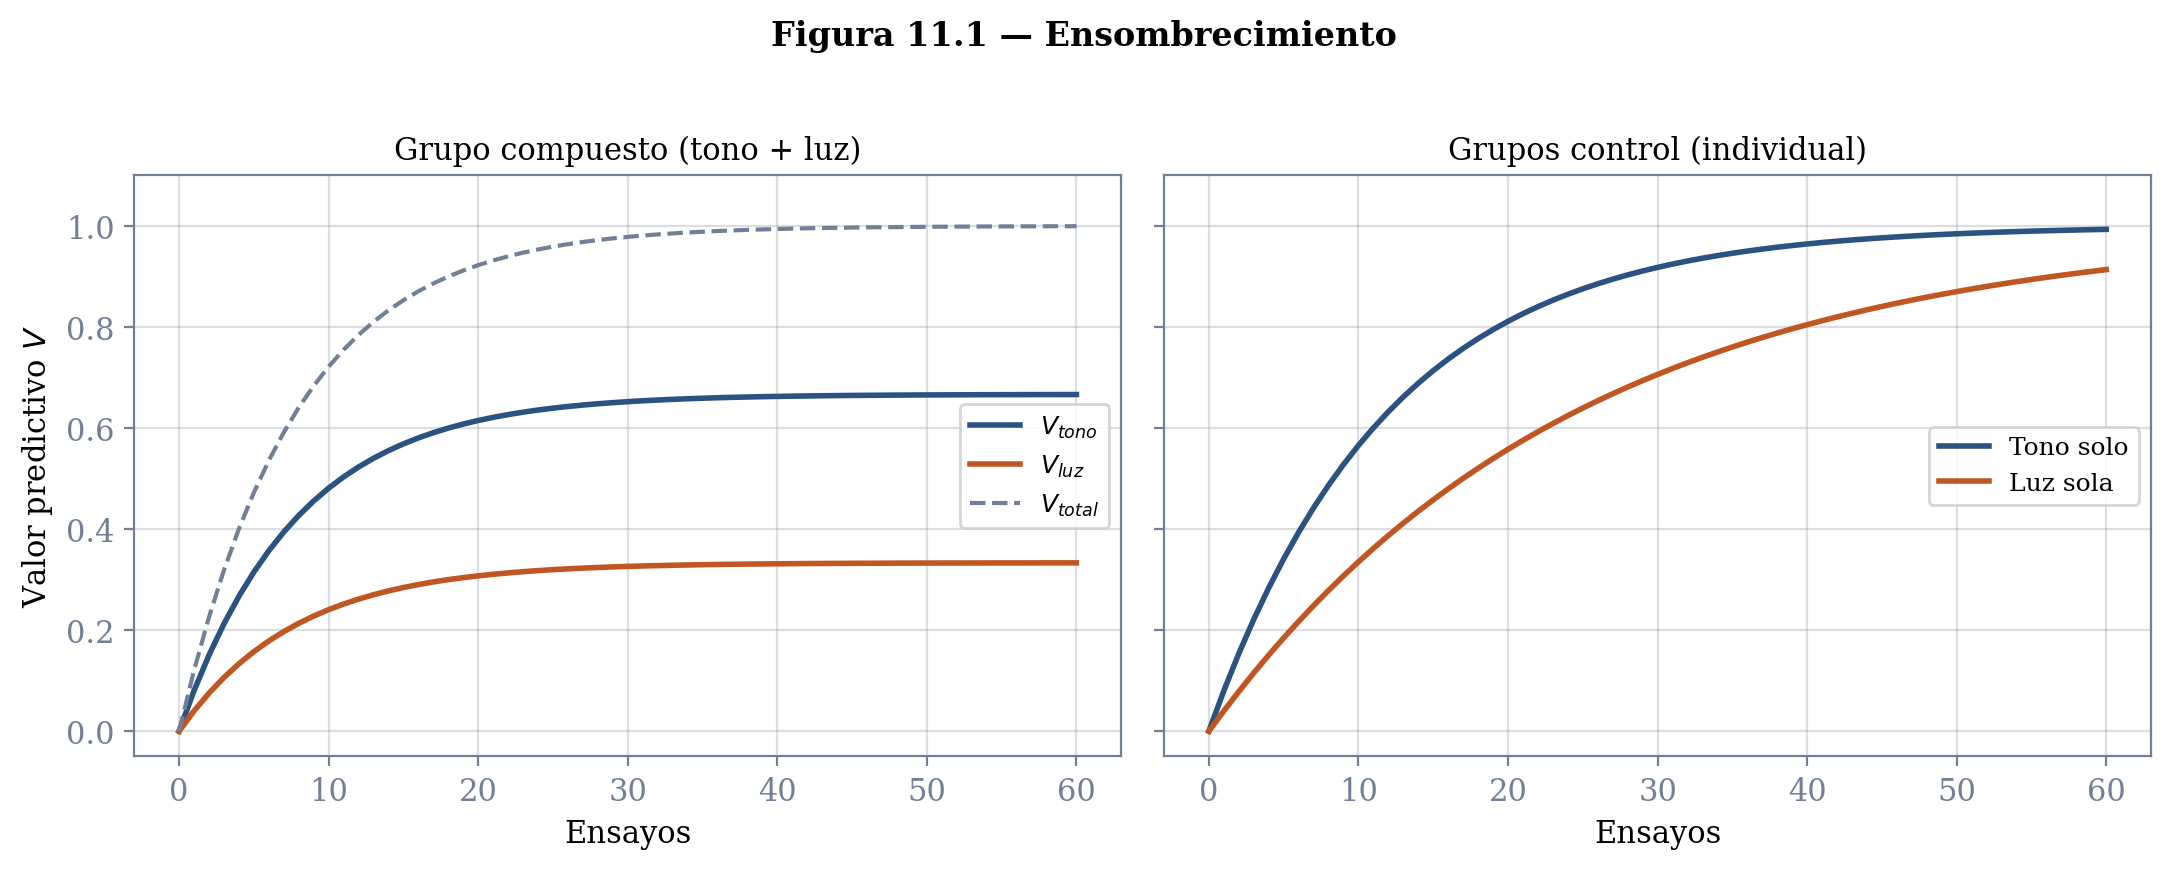
\includegraphics[width=7.8125in,height=\textheight,keepaspectratio]{Figuras/fig_11_1_ensombrecimiento.png}

}

\caption{\label{fig-ensombrecimiento}Ensombrecimiento}

\end{figure}%

\begin{quote}
\textbf{Note}

\emph{{[}Ensombrecimiento. Panel izquierdo: Grupo compuesto ---
evolución de \(V_{\text{tono}}\) (azul, \#2C5282, asíntota ≈ 0.67),
\(V_{\text{luz}}\) (naranja, \#C05621, asíntota ≈ 0.33) y
\(V_{\text{total}}\) (gris punteado, \#718096, asíntota ≈ 1.0) a lo
largo de 60 ensayos. Panel derecho: Grupos control ---
\(V_{\text{tono}}\) solo (azul) y \(V_{\text{luz}}\) sola (naranja),
ambos convergiendo a ≈ 1.0. Ejes: horizontal = ensayos, vertical = valor
predictivo V (0 a 1.0). Referencia visual: diapositiva 22 de
rescorla\_y\_Wagner\_2023.pptx.{]}}
\end{quote}

\mbox{}%
\section{Aplicación al bloqueo}\label{aplicaciuxf3n-al-bloqueo}

El bloqueo es quizás el resultado más importante que el modelo de
Rescorla y Wagner explica, y el que mejor ilustra la distancia entre
este modelo y cualquier versión que descanse en la mera contigüidad.

El protocolo tiene dos grupos, cuyo diseño conviene tener a la vista
antes de seguir el análisis:

{\def\LTcaptype{none} % do not increment counter
\begin{longtable}[]{@{}
  >{\raggedright\arraybackslash}p{(\linewidth - 4\tabcolsep) * \real{0.3043}}
  >{\raggedright\arraybackslash}p{(\linewidth - 4\tabcolsep) * \real{0.3478}}
  >{\raggedright\arraybackslash}p{(\linewidth - 4\tabcolsep) * \real{0.3478}}@{}}
\toprule\noalign{}
\begin{minipage}[b]{\linewidth}\raggedright
Grupo
\end{minipage} & \begin{minipage}[b]{\linewidth}\raggedright
Fase 1
\end{minipage} & \begin{minipage}[b]{\linewidth}\raggedright
Fase 2
\end{minipage} \\
\midrule\noalign{}
\endhead
\bottomrule\noalign{}
\endlastfoot
Bloqueo & Tono → Comida (60 ensayos) & Tono + Luz → Comida (60
ensayos) \\
Control & --- & Tono + Luz → Comida (60 ensayos) \\
\end{longtable}
}

Para el grupo de bloqueo, al final de la Fase 1 el tono ya predice
perfectamente la comida: \(V_{\text{tono}} \approx R\). En el primer
ensayo de la Fase 2, cuando aparecen el tono y la luz juntos seguidos de
comida, la predicción total es
\(V_{\text{total}} = V_{\text{tono}} + V_{\text{luz}} = R + 0 = R\). El
error de predicción es \(R - R = 0\). Sin error, no hay actualización.
La luz, a pesar de ser perfectamente contigua con el SBI, no adquiere
valor alguno.

La lógica es transparente una vez que se entiende la ecuación: cuando un
elemento ya predice el SBI, no queda error de predicción que pueda
asignarse a elementos nuevos. Computando explícitamente:

\[\Delta V_{\text{luz}} = \alpha\,\beta_{\text{luz}}\,(R - V_{\text{total}}) = \alpha\,\beta_{\text{luz}}\,(1 - 1) = 0\]

Para el grupo control, ambos estímulos parten de cero y compiten por el
valor disponible, produciendo un patrón similar al ensombrecimiento.

Noten que en la simulación del bloqueo, \(V_{\text{luz}}\) para el grupo
control no llega a 1 ---se detiene cerca de 0.4. La razón es la misma
que en el ensombrecimiento: el tono, al estar presente también, captura
parte del valor disponible.

\begin{figure}[H]

{\centering 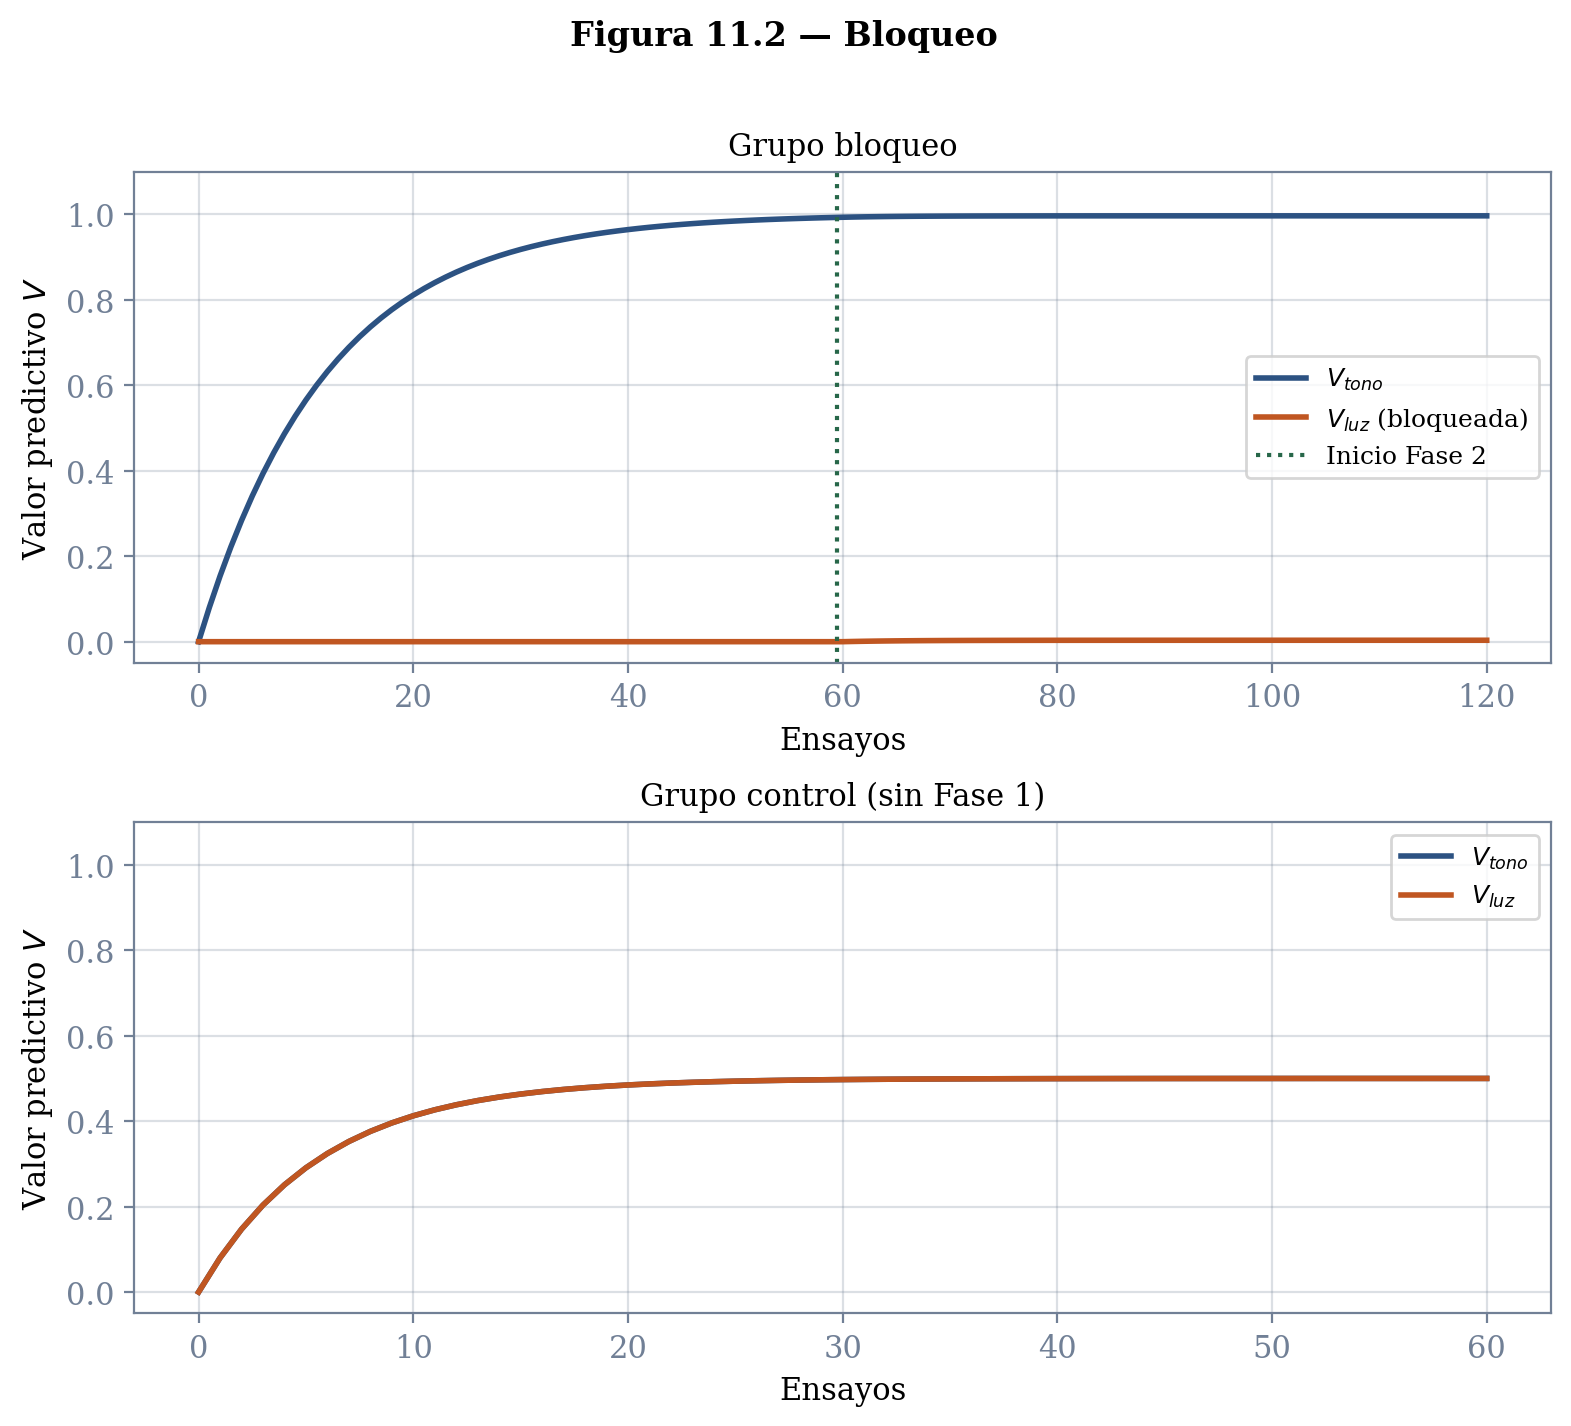
\includegraphics[width=7.8125in,height=\textheight,keepaspectratio]{Figuras/fig_11_2_bloqueo.png}

}

\caption{fig\_11\_2\_bloqueo}

\end{figure}%

\begin{quote}
\textbf{Note}

\emph{{[}Bloqueo. Panel superior: adquisición de \(V_{\text{tono}}\)
(azul, \#2C5282) durante la Fase 1, convergiendo a ≈ 1.0. Panel
inferior: Fase 2 --- \(V_{\text{luz}}\) del grupo bloqueo (naranja,
\#C05621, plana en ≈ 0) versus \(V_{\text{luz}}\) del grupo control
(verde, \#276749, creciente a ≈ 0.4). Línea divisoria vertical entre
fases. Ejes: horizontal = ensayos, vertical = valor predictivo V.
Referencia visual: diapositiva 24 de rescorla\_y\_Wagner\_2023.pptx.{]}}
\end{quote}

\mbox{}%
\section{Predicción contraintuitiva: la
sobreexpectación}\label{predicciuxf3n-contraintuitiva-la-sobreexpectaciuxf3n}

Cualquier versión del modelo de Bush y Mosteller predice que un SBI
adicional debe incrementar ---aunque sea por un monto pequeño--- el
valor predictivo de un estímulo. El modelo de Rescorla y Wagner predice
que en ciertas circunstancias ocurre exactamente lo contrario.

Consideremos el siguiente protocolo:

{\def\LTcaptype{none} % do not increment counter
\begin{longtable}[]{@{}lll@{}}
\toprule\noalign{}
Fase & Protocolo & Ensayos \\
\midrule\noalign{}
\endhead
\bottomrule\noalign{}
\endlastfoot
1 & Tono → Comida & 60 \\
2 & Luz → Comida & 60 \\
3 & Tono + Luz → Comida & 60 \\
\end{longtable}
}

Al final de las dos primeras fases, ambos estímulos han alcanzado la
asíntota: \(V_{\text{tono}} \approx 1\) y \(V_{\text{luz}} \approx 1\).
En la tercera fase, se presenta el compuesto tono + luz seguido de
comida.

Al inicio de la tercera fase,
\(V_{\text{total}} = V_{\text{tono}} + V_{\text{luz}} = 1 + 1 = 2\).
Pero el SBI vale \(R = 1\), porque solo aparece una porción de comida.
El error de predicción es \(R - V_{\text{total}} = 1 - 2 = -1\). El
error es \emph{negativo}: el organismo espera más de lo que obtiene. La
consecuencia es que ambos valores \emph{disminuyen} a pesar de que el
SBI está presente:

\[\Delta V_{\text{tono}} = \alpha\,\beta_{\text{tono}}\,(-1) < 0\]
\[\Delta V_{\text{luz}} = \alpha\,\beta_{\text{luz}}\,(-1) < 0\]

Los valores siguen disminuyendo hasta que su suma iguala al SBI:
\(V_{\text{tono}} + V_{\text{luz}} = 1\), en cuyo punto el error se hace
cero y el aprendizaje se detiene. Cada uno termina con un valor
aproximado de 0.5.

Esta predicción ---que reforzar un compuesto puede \emph{reducir} el
valor de sus elementos--- es imposible de generar sin el
\(V_{\text{total}}\). Un modelo con error individual siempre
incrementaría \(V\) cuando el SBI está presente. Interesantemente, la
predicción ha sido confirmada experimentalmente (Kremer, 1978; Rescorla,
2006), proporcionando fuerte evidencia a favor del modelo.

\begin{figure}[H]

{\centering 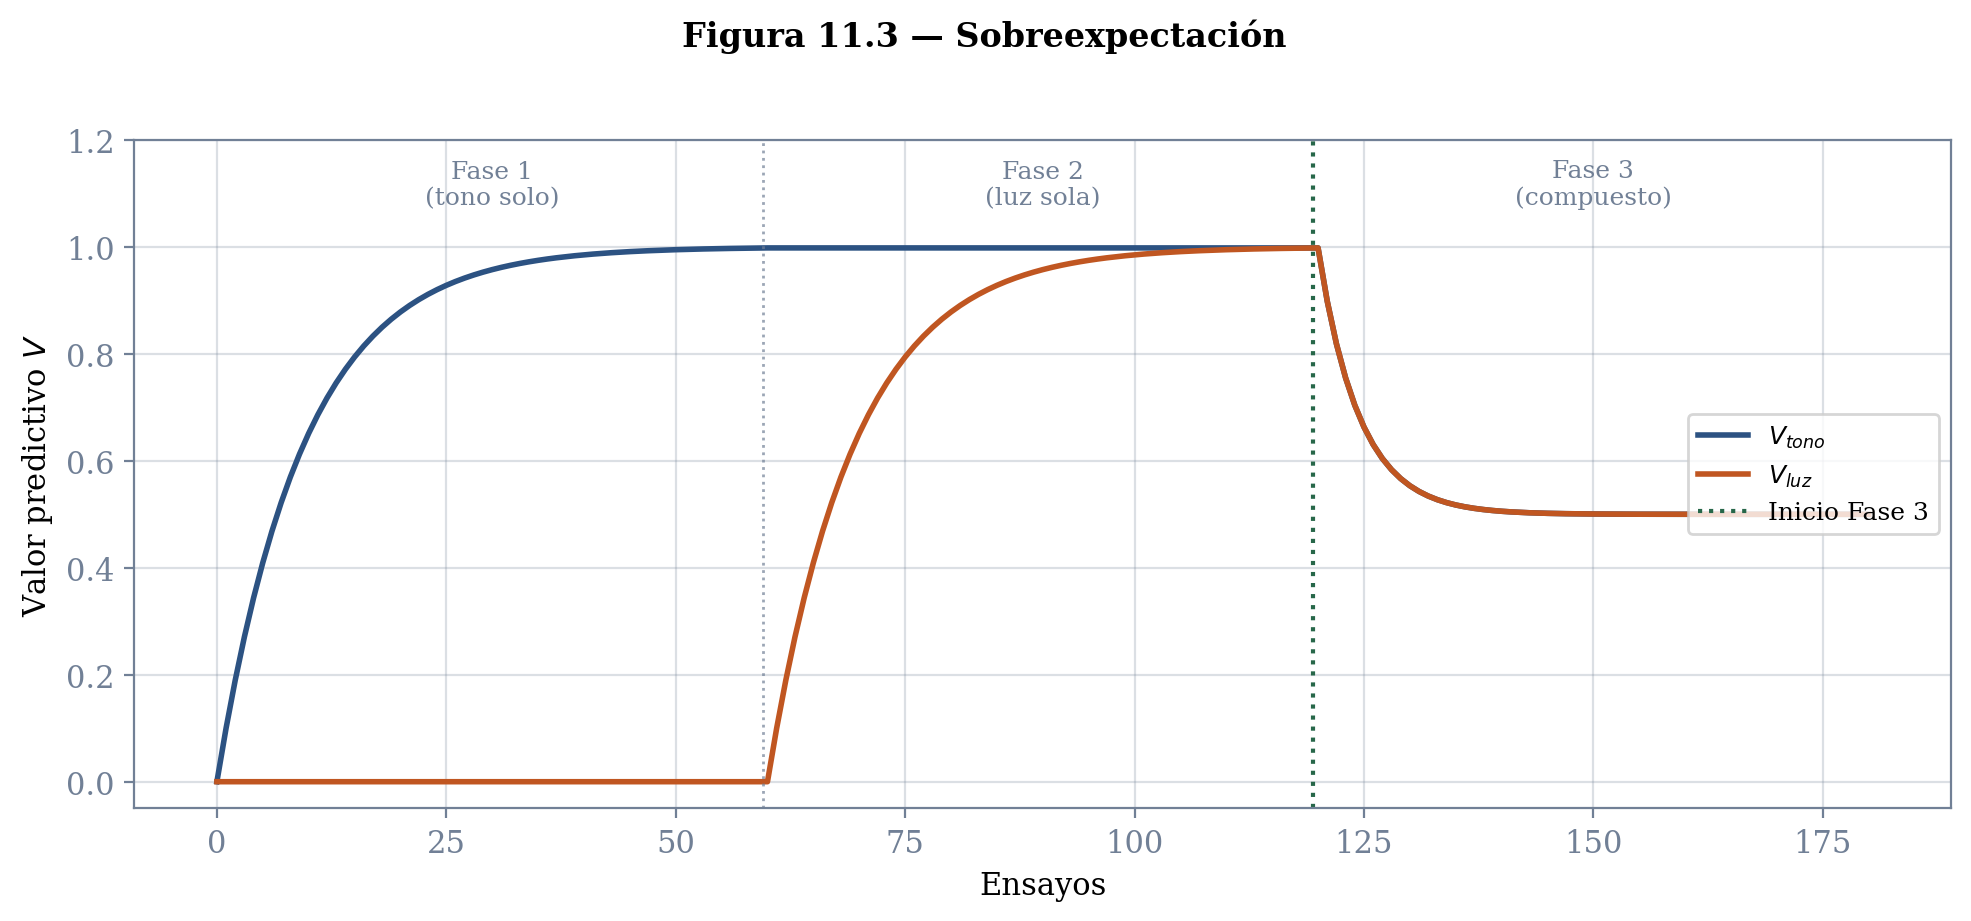
\includegraphics[width=7.8125in,height=\textheight,keepaspectratio]{Figuras/fig_11_3_sobreexpectacion.png}

}

\caption{fig\_11\_3\_sobreexpectacion}

\end{figure}%

\begin{quote}
\textbf{Note}

\emph{{[}Sobreexpectación. Panel izquierdo: curvas separadas de
\(V_{\text{tono}}\) y \(V_{\text{luz}}\) durante Fases 1 y 2
(adquisición individual, ambas convergen a 1.0). Panel derecho: Fase 3
--- ambos valores descienden desde 1.0 hasta ≈ 0.5 cuando se presentan
en compuesto. Colores: tono en azul (\#2C5282), luz en naranja
(\#C05621). Líneas verticales separando fases. Referencia visual:
diapositiva 26 de rescorla\_y\_Wagner\_2023.pptx.{]}}
\end{quote}

\begin{quote}
\textbf{Note}

Antes de continuar con la lectura, abre el
\href{https://colab.research.google.com/github/arbouria/Libro-ACA-2026/blob/main/Simuladores/Rescorla_Wagner.ipynb}{notebook
de simuladores de este capítulo (enlace a Google Colab)}. Contiene dos
simuladores interactivos que te permitirán explorar la ecuación de
Rescorla y Wagner con diferentes parámetros y protocolos.

El Simulador 11.1 se concentra en el ensombrecimiento. El Simulador 11.2
te permite seleccionar entre los protocolos que acabamos de analizar ---
adquisición simple, ensombrecimiento, bloqueo y sobreexpectación--- y
verificar que todos son consecuencias de la misma ecuación con
diferentes historias de entrenamiento. Usa los botones de ejemplo para
cargar configuraciones que producen resultados claros. El simulador
también incluye un protocolo de inhibición condicionada que te será útil
cuando llegues a la siguiente sección del capítulo. Después de leer
sobre cómo se crean los inhibidores y las pruebas de Rescorla, regresa
al simulador y explora ese protocolo: observa en la tabla numérica cómo
los ensayos A+ producen errores positivos y los ensayos AB− producen
errores negativos, y cómo esa alternancia es lo que permite que
\(V_B\)\hspace{0pt} descienda por debajo de cero.
\end{quote}

\mbox{}%
\section{Inhibición condicionada}\label{inhibiciuxf3n-condicionada}

Hasta este punto, hemos discutido estímulos que adquieren valor positivo
y predicen la presencia de un SBI. Pero ¿pueden los estímulos predecir
la \emph{ausencia} de un SBI? Poder hacer esa predicción tiene
importantes ventajas adaptativas. La señal de que un depredador no
aparecerá le permite a una presa buscar alimento sin interrupciones. La
señal de que no habrá comida le permite al organismo reorientar su
búsqueda hacia otros recursos. Al estudio de este fenómeno se le conoce
como \emph{inhibición condicionada}.

\mbox{}%
\subsection{Por qué un estímulo neutral no se convierte en
inhibidor}\label{por-quuxe9-un-estuxedmulo-neutral-no-se-convierte-en-inhibidor}

El estudio de la inhibición tardó décadas en despegar, y la estructura
del modelo original ayuda a entender por qué. Imaginen que se encuentran
con una persona paseando a un perro que los ignora completamente. El
perro no fue un SBI: ni les gruñó ni les movió la cola.
Consecuentemente, \(R = 0\). La persona era un desconocido que no
predice nada: su \(V\) es cero. El error de predicción es
\(R - V = 0 - 0 = 0\). No hay cambio. Si nada se espera y nada se
obtiene, nada se aprende. La persona sigue siendo un estímulo neutral,
no un inhibidor.

Esto establece una condición necesaria para la inhibición. Para que un
estímulo adquiera valor \emph{negativo}, el error de predicción debe ser
negativo. Para que eso ocurra cuando \(R = 0\), el estímulo debe
aparecer en compuesto con un estímulo que ya tiene valor positivo, de
tal forma que \(V_{\text{total}} > 0\) y el error
\((R - V_{\text{total}}) < 0\).

\mbox{}%
\subsection{Cómo se crea un
inhibidor}\label{cuxf3mo-se-crea-un-inhibidor}

Regresemos al ejemplo del perro, pero esta vez imaginemos que el perro
les gruñe de forma amenazante cada vez que ven a su paseador. Después de
muchos encuentros, la persona paseando al perro se convierte en un
predictor del gruñido: \(V_{\text{persona}} \approx 1\). En un siguiente
encuentro, la persona va acompañada de su pareja y el perro esta vez
\emph{no} gruñe. El error de predicción es
\(R - V_{\text{total}} = 0 - (V_{\text{persona}} + V_{\text{pareja}}) = 0 - (1 + 0) = -1\).
El error es negativo, y la pareja adquiere valor negativo:

\[\Delta V_{\text{pareja}} = \alpha\,\beta\,(-1) < 0\]

Después de muchos encuentros de este tipo ---la persona sola con perro
agresivo, la persona con pareja y perro tranquilo---, la pareja se
convierte en un inhibidor condicionado que predice la no ocurrencia del
gruñido. El proceso continúa hasta que la suma de valores en el
compuesto se aproxima a cero:
\(V_{\text{persona}} + V_{\text{pareja}} \approx 1 + (-1) = 0\), momento
en que el error desaparece.

\begin{figure}[H]

{\centering 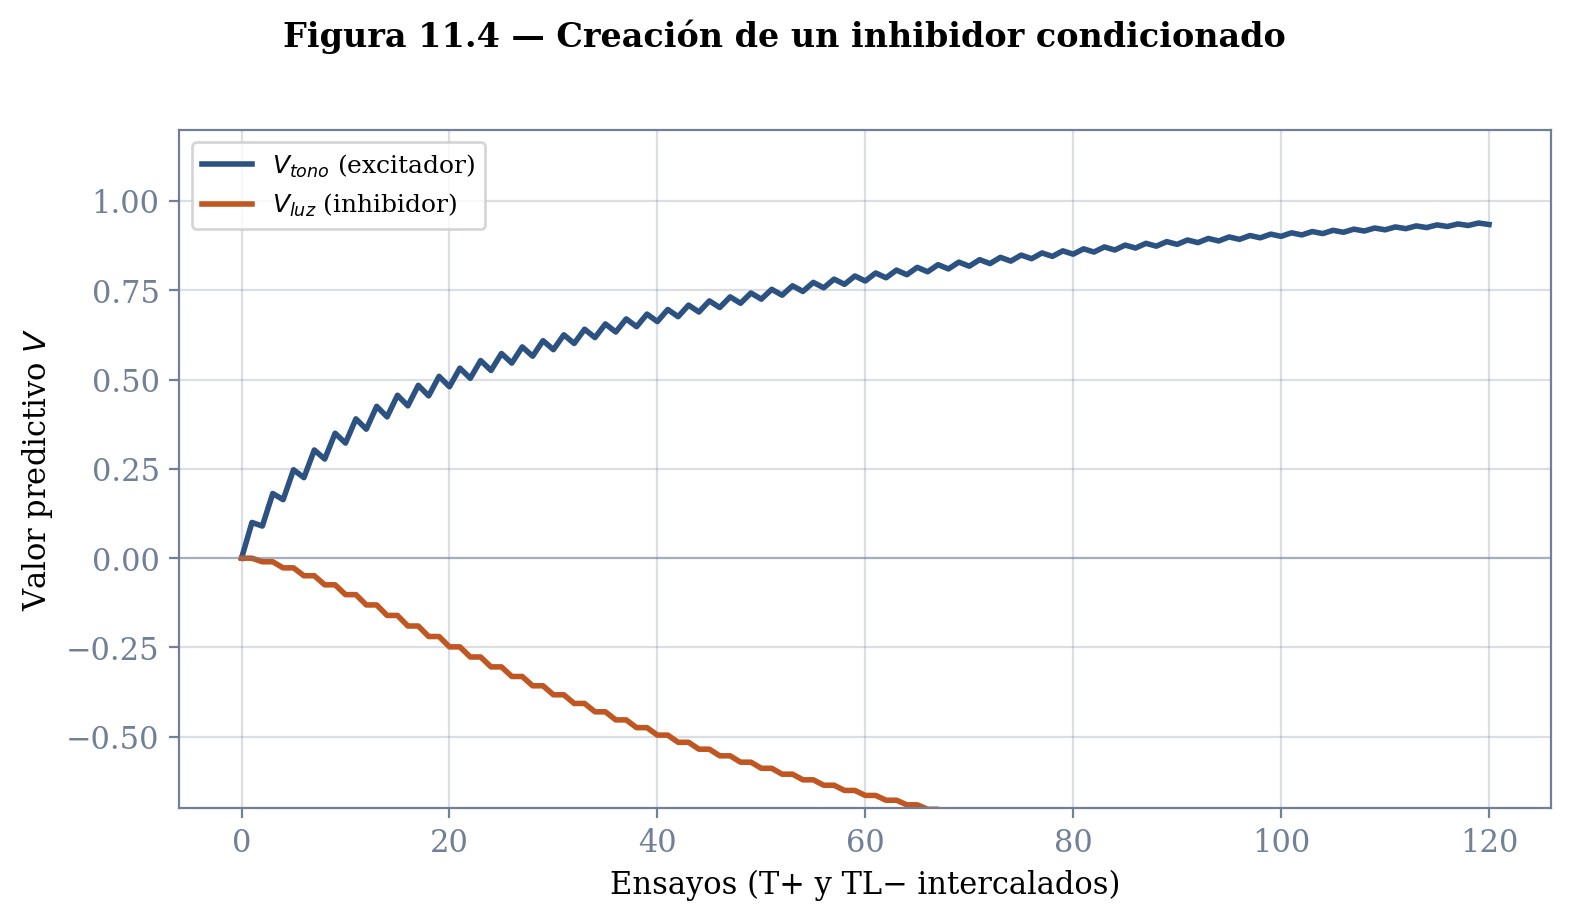
\includegraphics[width=0.9\linewidth,height=\textheight,keepaspectratio]{Figuras/fig_11_4_inhibidor.png}

}

\caption{fig\_11\_4\_inhibidor}

\end{figure}%

\begin{quote}
\textbf{Note}

\emph{{[}Creación de un inhibidor condicionado. Protocolo: Fase 1 ---
Tono+ (60 ensayos reforzados). Fase 2 --- Tono+ intercalados con TL−
(tono + luz sin SBI, 60 ensayos). Curvas: \(V_{\text{tono}}\) (azul,
\#2C5282, manteniéndose cerca de 1.0), \(V_{\text{luz}}\) (naranja,
\#C05621, descendiendo de 0 a ≈ −0.5). Eje vertical: valor predictivo
(−1.0 a 1.0). Referencia visual: figura superior de diapositiva 11 de
Inhibición\_Rescorla.pptx.{]}}
\end{quote}

\mbox{}%
\subsection{El problema empírico: ¿inhibidor o
neutral?}\label{el-problema-empuxedrico-inhibidor-o-neutral}

La segunda razón por la que la inhibición condicionada tardó en
estudiarse es la dificultad para distinguir empíricamente entre un
estímulo neutral ---que no predice nada--- y un estímulo que predice
\emph{la ausencia} de algo. Rescorla, en un artículo de 1969, propuso
que para concluir que un estímulo es un inhibidor condicionado, este
debe pasar dos pruebas complementarias.

En la primera, la \textbf{prueba de sumación}, se compara la respuesta
ante un estímulo excitador \(A\) presentado solo con la respuesta ante
el compuesto de \(A\) junto con el supuesto inhibidor \(X\). El
protocolo típico tiene tres fases:

{\def\LTcaptype{none} % do not increment counter
\begin{longtable}[]{@{}llll@{}}
\toprule\noalign{}
Grupo & Fase 1 & Fase 2 & Fase 3 (prueba) \\
\midrule\noalign{}
\endhead
\bottomrule\noalign{}
\endlastfoot
Inhibición & T+ / X+ & LT− & LX− \\
Control & T− / X+ & LT− & LX− \\
\end{longtable}
}

Si \(X\) es verdaderamente inhibitorio (\(V_X < 0\)), entonces
\(V_{\text{total}} = V_A + V_X < V_A\), y la respuesta al compuesto debe
ser menor que la respuesta a \(A\) solo. Regresando a nuestro ejemplo:
si la pareja del paseador es un inhibidor, el perro debería gruñir menos
cuando la pareja está presente que cuando el paseador va solo. Sin
embargo, Rescorla señala que estos resultados tienen una interpretación
alternativa: quizás la atención dirigida a \(X\) simplemente reduce la
atención dirigida a \(A\), produciendo una menor respuesta sin que \(X\)
sea genuinamente inhibitorio.

En la segunda, la \textbf{prueba de retardo}, se compara la velocidad de
adquisición de valor excitatorio entre el supuesto inhibidor \(X\) y un
estímulo neutral:

{\def\LTcaptype{none} % do not increment counter
\begin{longtable}[]{@{}llll@{}}
\toprule\noalign{}
Grupo & Fase 1 & Fase 2 & Fase 3 (prueba) \\
\midrule\noalign{}
\endhead
\bottomrule\noalign{}
\endlastfoot
Retardo & T+ & LT− & L+ \\
Control & T− & LT− & L+ \\
\end{longtable}
}

Si \(X\) tiene valor negativo, debe tardar más en alcanzar valores
positivos que un estímulo que parte de cero ---porque tiene que recorrer
mayor distancia. Pero también aquí hay una explicación alternativa:
quizás la familiaridad con \(X\) reduce la atención que recibe
(habituación), retardando el aprendizaje sin que el estímulo sea
inhibitorio.

La importancia del argumento de Rescorla es que las dos explicaciones
alternativas se contradicen entre sí. La alternativa para la sumación
requiere que \(X\) reciba \emph{más} atención (distrayendo de \(A\)); la
alternativa para el retardo requiere que \(X\) reciba \emph{menos}
atención (por habituación). No resulta plausible que un mismo estímulo
reciba más atención en una circunstancia y menos en otra. Si el estímulo
pasa ambas pruebas, las explicaciones atencionales se eliminan
mutuamente, y la conclusión de que \(X\) es genuinamente inhibitorio
queda como la más parsimoniosa.

\begin{figure}[H]

{\centering 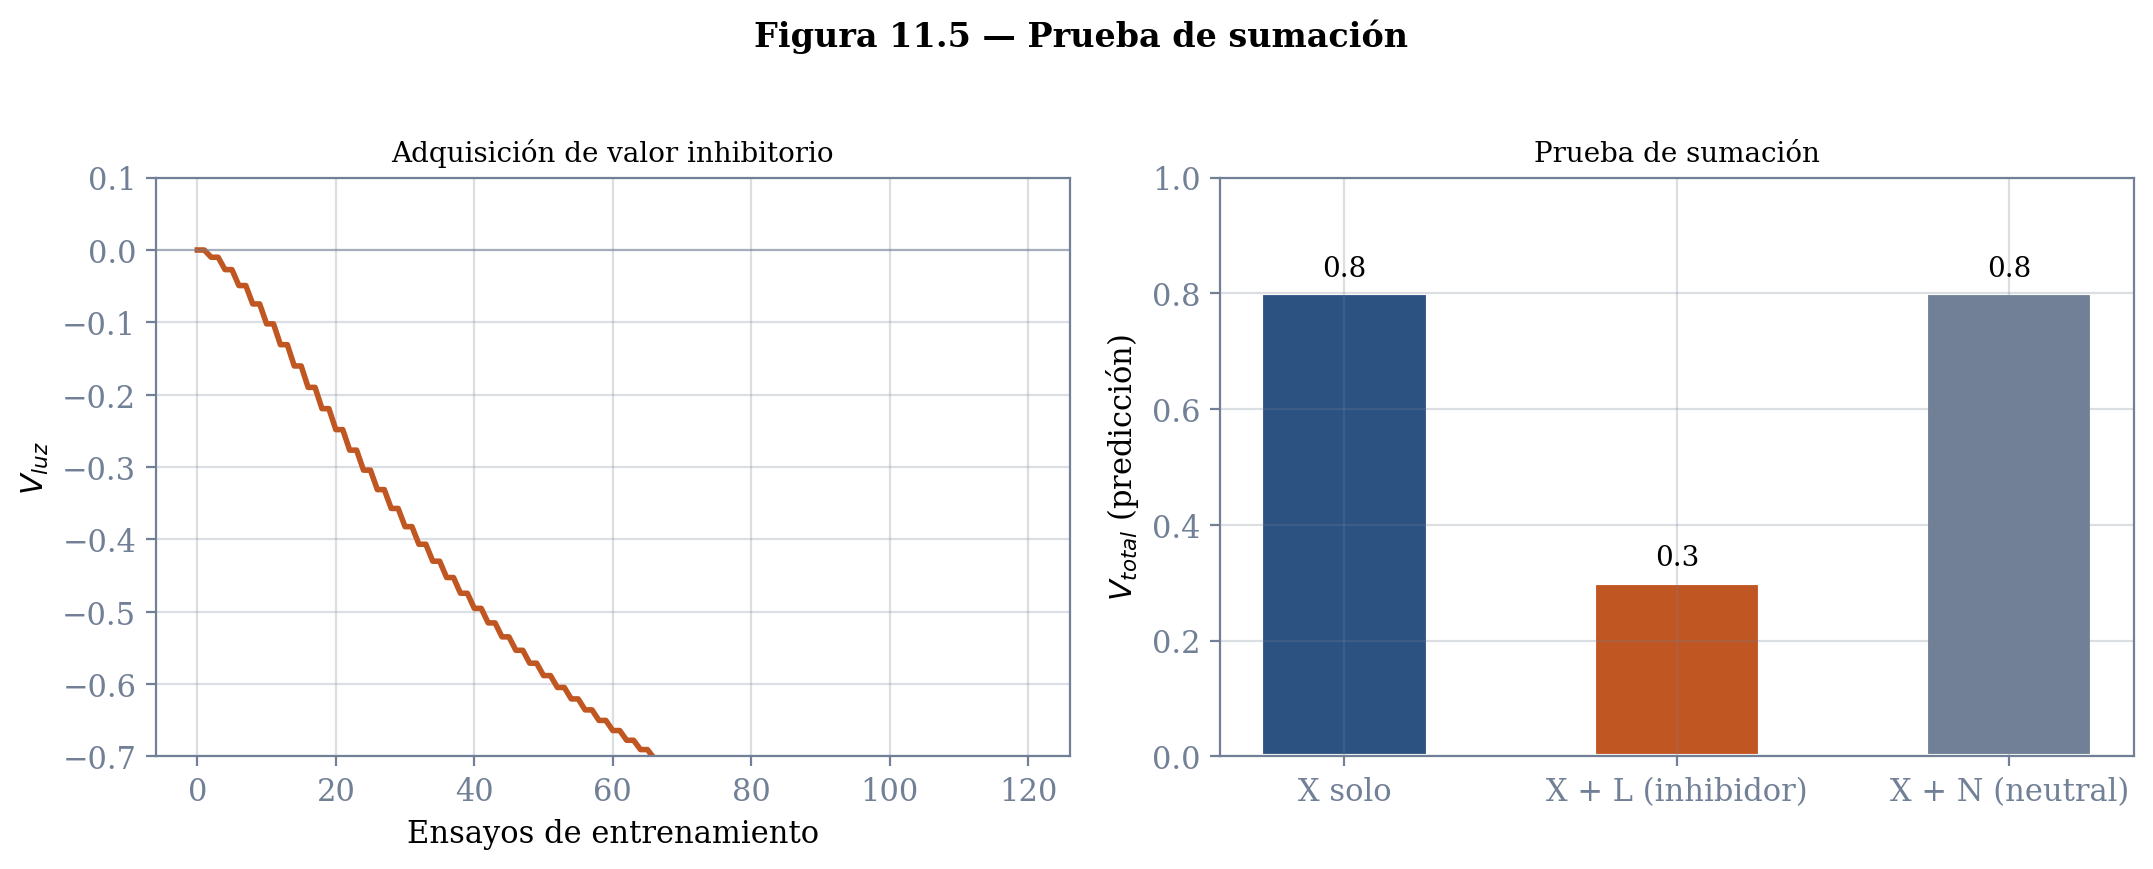
\includegraphics[width=7.8125in,height=\textheight,keepaspectratio]{Figuras/fig_11_5_sumacion.png}

}

\caption{fig\_11\_5\_sumacion}

\end{figure}%

\begin{quote}
\textbf{Note}

\emph{{[}Prueba de sumación. Panel superior: protocolo experimental en
tabla (Grupo Inhibición: Fase 1 = T+/X+, Fase 2 = LT−, Fase 3 = LX−;
Grupo Control: Fase 1 = T−/X+, Fase 2 = LT−, Fase 3 = LX−). Panel
inferior izquierdo: adquisición de \(V_{\text{luz}}\) (valor negativo,
convergiendo a ≈ −0.5 durante Fase 2). Panel inferior derecho: respuesta
al compuesto LX en Fase 3 --- grupo inhibición (naranja, menor
respuesta) vs.~grupo control (verde, mayor respuesta). Referencia
visual: diapositiva 11 de Inhibición\_Rescorla.pptx.{]}}

::;

\begin{figure}[H]

{\centering 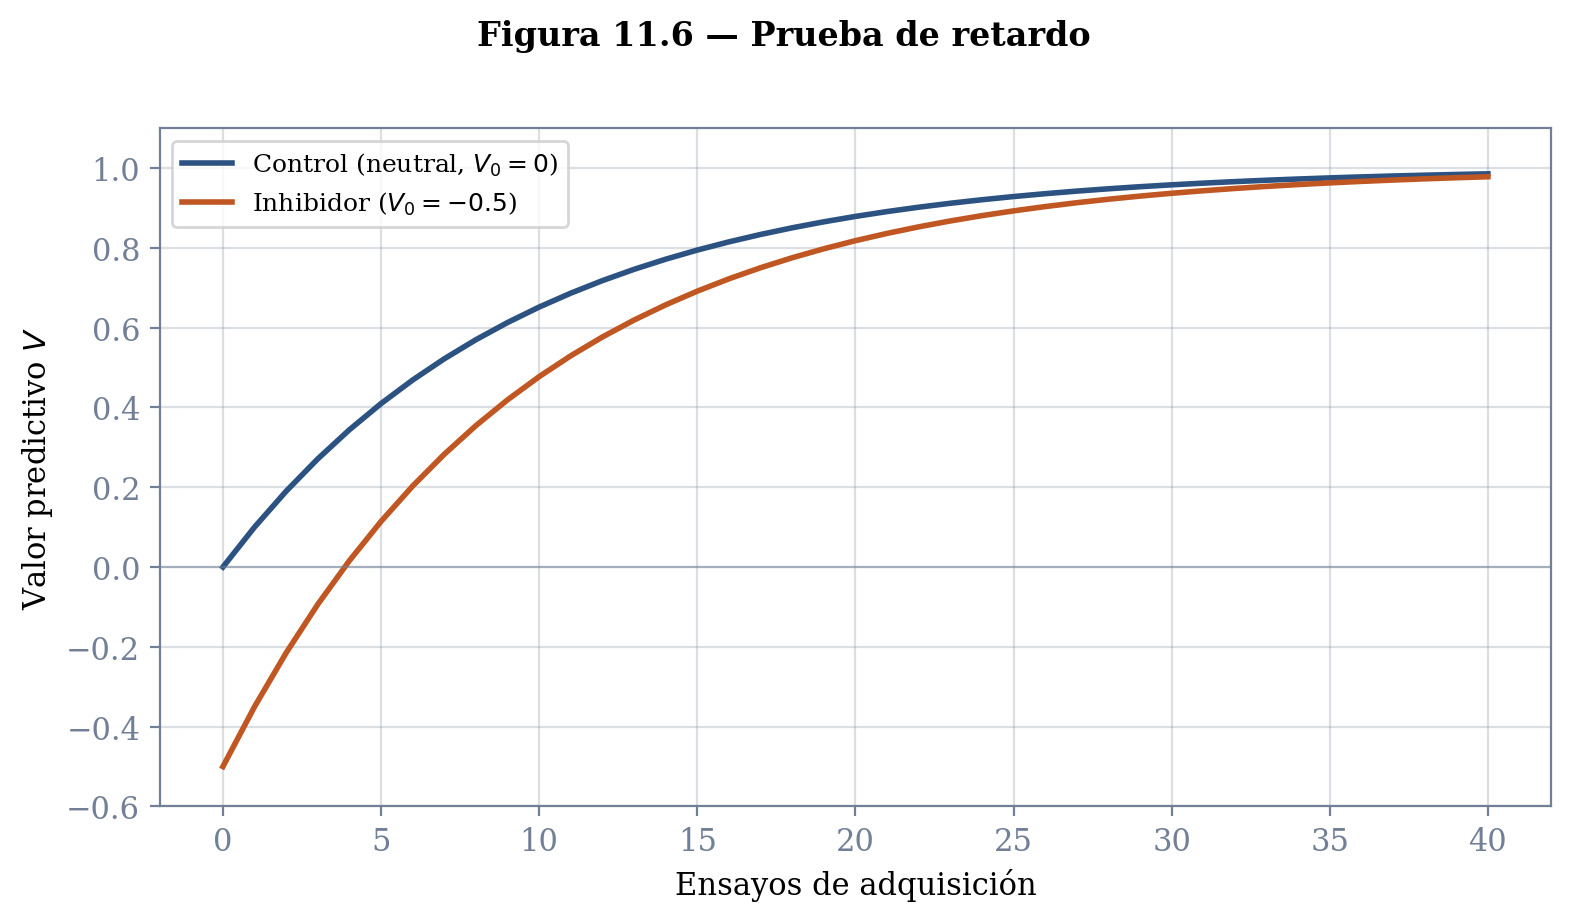
\includegraphics[width=7.8125in,height=\textheight,keepaspectratio]{Figuras/fig_11_6_retardo.png}

}

\caption{fig\_11\_6\_retardo}

\end{figure}%

\begin{quote}
\textbf{Note}

\emph{{[}Prueba de retardo. Panel superior: protocolo (Grupo Retardo:
Fase 1 = T+, Fase 2 = LT−, Fase 3 = L+; Grupo Control: Fase 1 = T−, Fase
2 = LT−, Fase 3 = L+). Panel inferior: curvas de adquisición en Fase 3
--- \(V_{\text{luz}}\) del grupo retardo (naranja, \#C05621, partiendo
de ≈ −0.5, adquisición lenta) vs.~\(V_{\text{luz}}\) del grupo control
(azul, \#2C5282, partiendo de 0, adquisición rápida). Referencia visual:
diapositiva 13 de Inhibición\_Rescorla.pptx.{]}}
\end{quote}

\mbox{}%
\section{Limitaciones del modelo}\label{limitaciones-del-modelo}

Dentro de la psicología, pocos modelos han sido tan exitosos como el de
Rescorla y Wagner en dar cuenta de una amplia gama de resultados, abrir
nuevas rutas de investigación y capturar formalmente el papel del error
de predicción en el aprendizaje. Sin embargo, como ocurre con cualquier
modelo, hay predicciones que no se sostienen empíricamente. Estas fallas
no son fracasos sino pistas: cada una ha señalado hacia direcciones que
enriquecieron la comprensión del aprendizaje. Presentamos tres que, por
su claridad conceptual y por las alternativas que motivaron, merecen
atención.

\mbox{}%
\subsection{La extinción no reduce el valor a
cero}\label{la-extinciuxf3n-no-reduce-el-valor-a-cero}

En extinción, el SBI que previamente seguía al estímulo deja de
presentarse. En este caso \(R = 0\), y el modelo predice que \(V\)
disminuirá hasta igualarse a \(R\), es decir, hasta llegar a cero.
Cuando eso ocurre, el error de predicción desaparece (\(0 - 0 = 0\)) y
no hay más cambios. Para el modelo, un estímulo extinguido y un estímulo
que nunca fue condicionado son funcionalmente idénticos: ambos tienen
\(V = 0\).

La evidencia dice otra cosa. Hay una multitud de reportes que muestran
que el mero paso del tiempo produce una \emph{recuperación espontánea}
de la respuesta condicionada extinguida. Adicionalmente, estímulos
previamente extinguidos adquieren valor excitatorio más rápido que
estímulos genuinamente neutrales, a pesar de que se supone que ambos
parten de \(V = 0\). Estos hallazgos sugieren que la extinción no borra
la asociación original sino que es sensible al contexto. Esta literatura
y los modelos para dar cuenta de ella los presentaremos en un capítulo
posterior sobre extinción y contexto.

\mbox{}%
\subsection{La inhibición condicionada no se
extingue}\label{la-inhibiciuxf3n-condicionada-no-se-extingue}

Si la excitación y la inhibición son simétricas ---si \(V\) puede subir
y bajar por la misma escala continua---, entonces un inhibidor
condicionado (\(V < 0\)) debería poder extinguirse de la misma manera
que un excitador: presentándolo sin SBI hasta que \(V\) regrese a cero.
El modelo predice exactamente eso: cuando un inhibidor con \(V = -0.5\)
se presenta solo sin SBI, el error de predicción es
\(0 - (-0.5) = 0.5 > 0\), y el valor debería subir hacia cero.

Sin embargo, la evidencia empírica muestra que presentar un inhibidor
condicionado sin consecuencias \emph{no reduce} su valor inhibitorio. El
inhibidor mantiene su efecto en pruebas de sumación y retardo
posteriores, como si la fase de extinción no hubiera ocurrido. Este
resultado sugiere que la inhibición puede ser cualitativamente diferente
de la excitación, no simplemente el extremo negativo de una misma
dimensión.

\begin{figure}[H]

{\centering 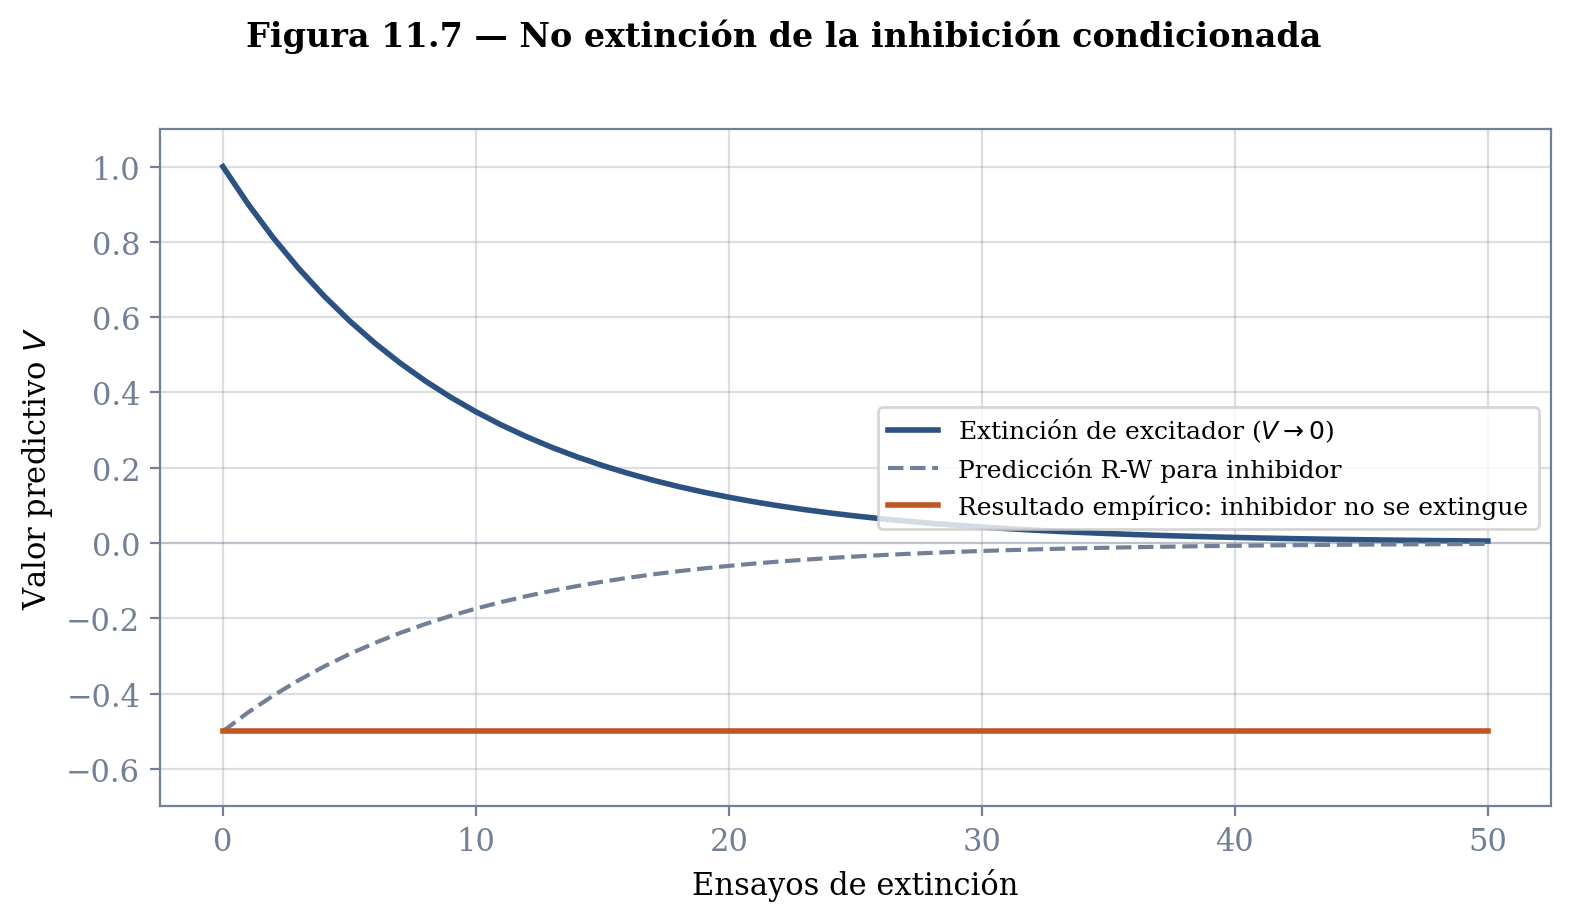
\includegraphics[width=7.8125in,height=\textheight,keepaspectratio]{Figuras/fig_11_7_no_extincion_inhibicion.png}

}

\caption{fig\_11\_7\_no\_extincion\_inhibicion}

\end{figure}%

\begin{quote}
\textbf{Note}

\emph{No extinción de inhibición. Protocolo: Fase 1 = creación del
inhibidor (T+/LT−); Fase 2 = presentación de L solo (intento de
extinción); Fase 3 = prueba de sumación. Dos curvas superpuestas:
extinción de un excitador (azul, \#2C5282, \(V\) desciende de ≈ 1.0 a ≈
0) y ``extinción'' de un inhibidor (naranja, \#C05621, \(V\) se mantiene
cerca de −0.5). El modelo predice que ambas converjan a cero;
empíricamente, solo la primera lo hace. Referencia visual: diapositiva 4
de Problemas\_con\_el\_modelo.pptx.{]}}
\end{quote}

\mbox{}%
\subsection{Inhibición latente}\label{inhibiciuxf3n-latente}

Consideremos un protocolo simple. A un grupo se le presenta, durante 60
ensayos, un estímulo neutral sin SBI; en una segunda fase, ese mismo
estímulo es seguido de un SBI. A un grupo control solo se le presenta la
segunda fase. Para el modelo de Rescorla y Wagner, la primera fase no
debería tener efecto: si \(V = 0\) y \(R = 0\), entonces el error es
cero y \(V\) permanece en cero. Ambos grupos deberían aprender a la
misma velocidad en la segunda fase.

Sin embargo, una enorme literatura reporta que la pre-exposición a un
estímulo sin consecuencias \emph{retarda} la adquisición posterior de
valor predictivo. A este fenómeno se le conoce como \emph{inhibición
latente}, y el modelo de Rescorla y Wagner no puede explicarlo porque
asume que \(\beta\) ---la asociabilidad del estímulo--- es fija. El
hallazgo sugiere que la pre-exposición reduce \(\beta\): el estímulo
``pierde la atención'' del organismo porque ha aprendido que no predice
nada importante. Cuando en la segunda fase el estímulo sí va seguido de
un SBI, el sistema tarda en ``prestarle atención'' de nuevo.

Este fenómeno fue la motivación principal para modelos alternativos que
enfatizan cambios dinámicos en la atención, y no solo en el valor
asociativo. El más influyente de estos modelos es el de Pearce y Hall
(1980), cuya idea central es que la atención a un estímulo (\(\beta\))
no es fija sino que depende de si ese estímulo ha sido seguido de
eventos sorpresivos. Cuando un estímulo predice bien lo que ocurre
(error bajo), la atención que recibe disminuye; cuando lo que ocurre es
inesperado (error alto), la atención aumenta. En un capítulo posterior,
cuando examinemos modelos bayesianos del aprendizaje, veremos cómo esta
idea se formaliza de manera más general: el organismo no solo actualiza
lo que cree (\(V\)), sino también cuánta confianza tiene en lo que cree,
y cuánta atención dedica a recoger nueva evidencia.

\begin{figure}[H]

{\centering 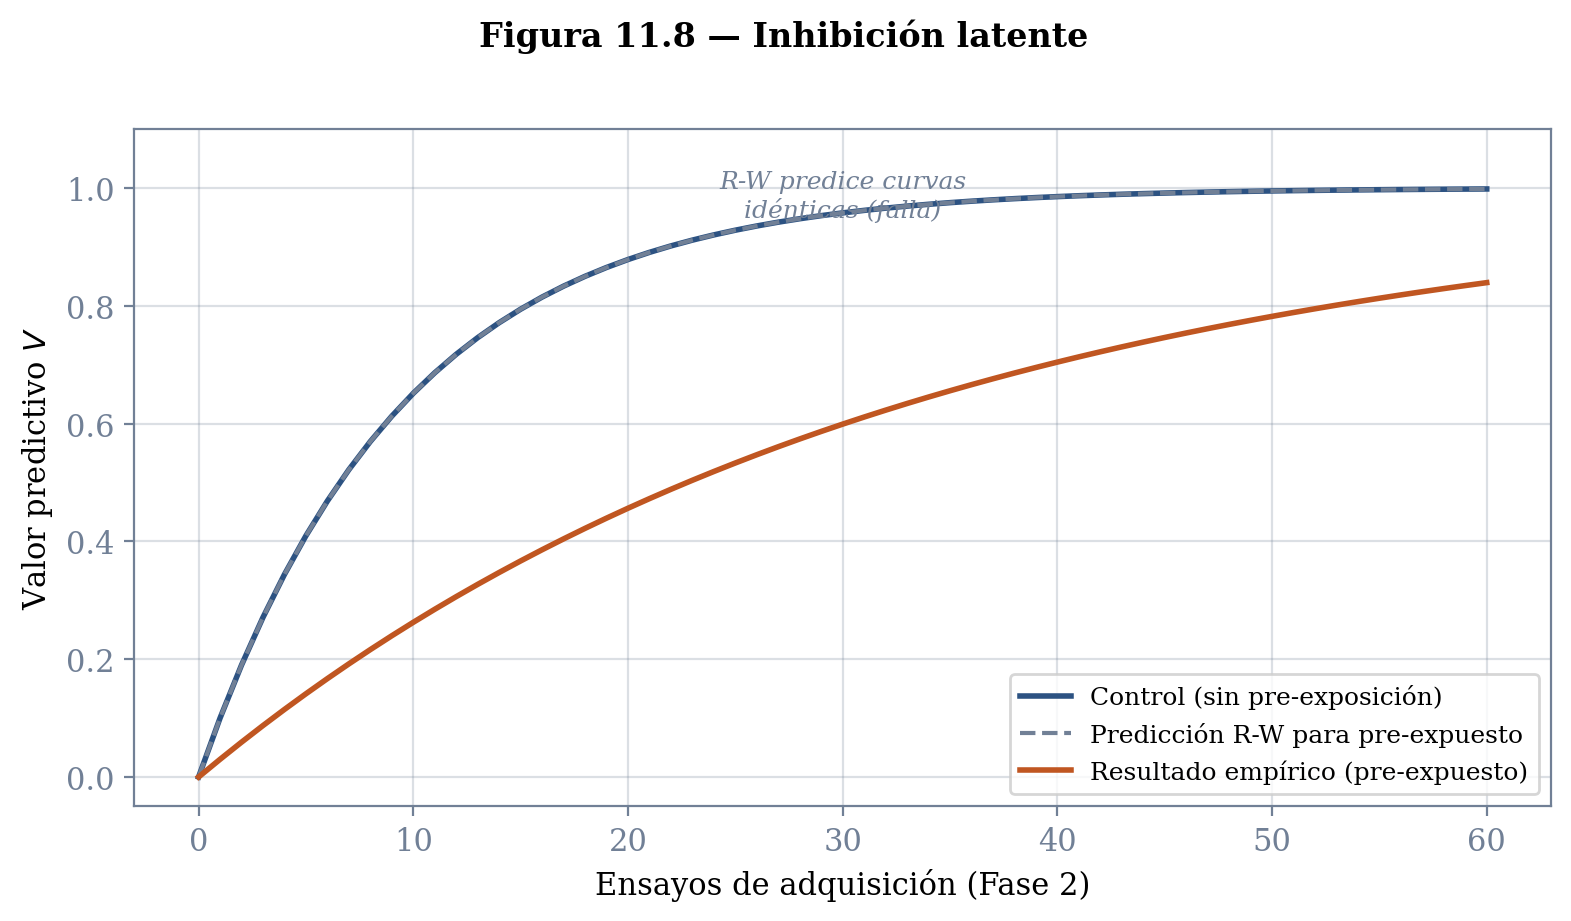
\includegraphics[width=7.8125in,height=\textheight,keepaspectratio]{Figuras/fig_11_8_inhibicion_latente.png}

}

\caption{fig\_11\_8\_inhibicion\_latente}

\end{figure}%

\begin{quote}
\textbf{Note}

\emph{{[}Inhibición latente. Dos curvas de adquisición en Fase 2: grupo
pre-expuesto (naranja, \#C05621, adquisición lenta) vs.~grupo control
sin pre-exposición (azul, \#2C5282, adquisición rápida). Ambos empiezan
con \(V = 0\); la diferencia no se explica por el modelo de R\&W. Línea
vertical separando fases. Eje horizontal = ensayos, vertical = valor
predictivo V (0 a 1.0).{]}}
\end{quote}

\mbox{}%
\section{Conexiones}\label{conexiones-4}

\mbox{}%
\subsection{El comparador universal: de la selección natural a
Rescorla-Wagner}\label{el-comparador-universal-de-la-selecciuxf3n-natural-a-rescorla-wagner}

A lo largo de los bloques anteriores hemos encontrado, una y otra vez,
la misma arquitectura formal: un sistema que compara dos cantidades,
detecta una diferencia, y usa esa diferencia para ajustar su estado. En
la selección natural, la ecuación de Price formaliza la covarianza entre
un rasgo y el éxito reproductivo --- la diferencia entre el individuo y
el promedio poblacional, ponderada por el fitness, impulsa el cambio
evolutivo. En la kinesis, el organismo compara su estado presente con su
estado inmediatamente anterior y cambia de explorar a explotar. En las
taxias, la comparación es simultánea --- entre dos puntos del espacio
--- y el ajuste es una orientación. En los sistemas de
retroalimentación, un comparador contrasta el valor actual de una
variable con un punto de referencia y genera una señal de error que
corrige la desviación.

El modelo de Bush y Mosteller llevó esta misma operación al aprendizaje:
el organismo compara lo que obtuvo (\(R\)) con lo que esperaba obtener
(\(V\)), y esa diferencia --- el error de predicción --- impulsa la
actualización. Lo que cambia respecto a los mecanismos anteriores es la
fuente de la referencia: ya no es el estado inmediato ni un punto fijo
genético, sino una memoria de largo plazo que integra la experiencia
acumulada.

El modelo de Rescorla y Wagner extiende esa misma operación a un
escenario más complejo: la referencia ya no es el valor de un solo
evento sino la suma de los valores de todos los eventos presentes
simultáneamente. El error sigue siendo una diferencia entre lo obtenido
y lo esperado, pero ahora lo esperado refleja la contribución conjunta
de múltiples predictores. La competencia entre estímulos no es un
mecanismo nuevo --- es la consecuencia de aplicar el mismo principio de
reducción de diferencia a un mundo con múltiples fuentes de información.
En todos los casos --- selección natural, kinesis, retroalimentación,
Bush y Mosteller, Rescorla y Wagner --- el motor del cambio es la
discrepancia, y el equilibrio se alcanza cuando esa discrepancia
desaparece.

\mbox{}%
\subsection{Hacia atrás: Bush y Mosteller y la asignación de
crédito}\label{hacia-atruxe1s-bush-y-mosteller-y-la-asignaciuxf3n-de-cruxe9dito}

El modelo de Rescorla y Wagner resuelve el problema que el capítulo
anterior dejó explícitamente abierto. Bush y Mosteller formalizaron el
error de predicción como motor del aprendizaje, pero su ecuación opera
sobre eventos individuales. Cuando hay varios estímulos presentes, cada
uno actualizaría su valor de manera independiente y fenómenos como el
bloqueo no se derivan. Rescorla y Wagner resolvieron esto con una
extensión que, en retrospectiva, es la más natural posible: computar el
error sobre la suma de todos los valores presentes. Esa suma
(\(V_{\text{total}}\)) convierte la competencia entre estímulos en
consecuencia matemática de la misma ecuación de error de predicción.

El bloqueo de Kamin, que en el capítulo sobre asignación de crédito a
estímulos establecimos como la evidencia central, encuentra aquí su
explicación formal: si un elemento ya predice perfectamente el SBI, la
suma de valores iguala a \(R\), el error es cero, y ningún estímulo
nuevo puede adquirir valor. El ensombrecimiento y la sobreexpectación
emergen por la misma lógica. No son fenómenos independientes que
requieran explicaciones separadas sino manifestaciones distintas de un
mismo principio.

\mbox{}%
\subsection{Hacia adelante: Correlaciones, tiempo y modelos
bayesianos}\label{hacia-adelante-correlaciones-tiempo-y-modelos-bayesianos}

El modelo de Rescorla y Wagner asume que el aprendizaje ocurre ensayo a
ensayo, en tiempo discreto. Pero los organismos experimentan el tiempo
como un flujo continuo, no como una secuencia de ensayos empaquetados.
En un capítulo posterior examinaremos los experimentos de Rescorla sobre
correlaciones y contingencias --- P(SBI\textbar EC) versus
P(SBI\textbar¬EC) --- y veremos cómo el modelo de Gallistel reformula el
problema del aprendizaje en términos de tasas de eventos en el tiempo,
no de asociaciones ensayo a ensayo. Esa reformulación cambiará
profundamente la pregunta: de ``¿cuánta fuerza tiene la asociación?'' a
``¿ha cambiado la tasa de refuerzo?''.

Las limitaciones que identificamos --- la incapacidad de explicar la
extinción como proceso reversible, la asimetría entre excitación e
inhibición, y la insensibilidad a la pre-exposición --- apuntan todas
hacia una misma dirección: el organismo no solo actualiza lo que cree,
sino que también ajusta la confianza de sus creencias y la atención que
dedica a recoger evidencia. Esa idea, esbozada por Pearce y Hall y
formalizada con mayor rigor en modelos bayesianos, será tema de
capítulos posteriores.

Hay una segunda línea de extensión que también examinaremos más
adelante. La ecuación de Rescorla y Wagner opera ensayo a ensayo,
comparando lo obtenido con lo esperado en el momento presente. Pero en
muchas situaciones el SBI aparece al final de una secuencia de acciones,
no inmediatamente después del estímulo. Las extensiones de la ecuación
al caso temporal --- en particular, el aprendizaje por diferencias
temporales (TD-learning) de Sutton y Barto --- resuelven ese problema
permitiendo que la señal de error se propague hacia atrás en el tiempo,
y resultan ser formalmente equivalentes a la señal de las neuronas
dopaminérgicas descubierta por Schultz y colaboradores. Esa conexión
entre la psicología del aprendizaje, la neurociencia y el aprendizaje
automático la desarrollaremos cuando abordemos el aprendizaje
secuencial.

\mbox{}%
\section{Resumen}\label{resumen-5}

El modelo de Rescorla y Wagner extiende el modelo de Bush y Mosteller a
estímulos compuestos mediante un supuesto que es a la vez simple y
poderoso: los estímulos son separables en elementos, y el error de
predicción se computa sobre la suma de los valores de todos los
elementos presentes. Esa modificación genera competencia entre estímulos
como consecuencia matemática y da cuenta del ensombrecimiento, el
bloqueo, la sobreexpectación y la inhibición condicionada sin invocar
mecanismos adicionales.

El modelo tiene limitaciones. No explica la recuperación espontánea tras
la extinción, la resistencia de la inhibición condicionada a la
extinción, ni el efecto de retardo por pre-exposición (inhibición
latente). Cada una de estas fallas señala hacia mecanismos que el modelo
no contempla: la sensibilidad al contexto, la posible asimetría entre
excitación e inhibición, y los cambios dinámicos en la atención al
estímulo. El modelo de Pearce y Hall propone que la atención (\(\beta\))
no es fija sino que varía con la historia de sorpresas; modelos
bayesianos posteriores formalizan esa idea de manera más general.

A pesar de estas limitaciones, la ecuación de Rescorla y Wagner sigue
siendo, después de más de cincuenta años, el punto de partida obligado
para cualquier discusión formal sobre el aprendizaje asociativo. Su
legado no está solo en lo que explica sino en lo que sus fallas
revelaron: que el aprendizaje es más rico de lo que cualquier ecuación
de una sola línea puede capturar.

\begin{center}\rule{0.5\linewidth}{0.5pt}\end{center}

\mbox{}%
\section{Ejercicios}\label{ejercicios-3}

\textbf{1.} Para cada uno de los siguientes escenarios, indica si los
modelos de Bush y Mosteller y Rescorla y Wagner hacen predicciones
idénticas o diferentes, y explica por qué: (a) un tono se presenta 60
veces seguido de comida; (b) un tono se presenta 60 veces junto con una
luz, ambos seguidos de comida; (c) primero un tono solo se presenta 60
veces con comida, luego el tono junto con una luz se presentan 60 veces
con comida.

\textbf{2.} Con \(\alpha = 0.2\), \(\beta_{\text{tono}} = 0.4\),
\(\beta_{\text{luz}} = 0.3\), y \(R = 1\), calcula los primeros tres
ensayos de un protocolo de ensombrecimiento (tono + luz → comida). Para
cada ensayo reporta: \(V_{\text{total}}\), error de predicción,
\(\Delta V_{\text{tono}}\), \(\Delta V_{\text{luz}}\), y los nuevos
valores. ¿Qué patrón se empieza a observar?

\textbf{3.} Usa el Simulador 11.2 para comparar el resultado del bloqueo
cuando la intensidad del SBI cambia entre fases. Configura el protocolo
de bloqueo estándar (Fase 1: tono → comida con \(R = 1\); Fase 2: tono +
luz → comida con \(R = 1\)). Ahora repite con \(R = 1.5\) en la Fase 2,
manteniendo \(R = 1\) en la Fase 1. ¿Qué ocurre con \(V_{\text{luz}}\)?
Este fenómeno, llamado \emph{desbloqueo}, fue una de las primeras
confirmaciones experimentales del modelo. Explica en términos del error
de predicción por qué el cambio en la intensidad del SBI ``desbloquea''
el aprendizaje.

\textbf{4.} Explica en tus propias palabras por qué un inhibidor
condicionado solo puede formarse en presencia de un excitador. Luego,
usando la lógica de Rescorla sobre las pruebas de sumación y retardo,
explica por qué se necesitan \emph{ambas} pruebas para concluir que un
estímulo es genuinamente inhibitorio.

\textbf{5.} El modelo de Rescorla y Wagner predice que un estímulo
extinguido y un estímulo genuinamente neutral son funcionalmente
idénticos. Sin embargo, la evidencia muestra recuperación espontánea y
readquisición rápida del estímulo extinguido. ¿Qué implica esto sobre lo
que ``sabe'' el organismo al final de la extinción? ¿La extinción es
``desaprendizaje'' o algo diferente?

\textbf{6.} \emph{(Reflexión)} El modelo de Rescorla y Wagner supone que
\(\beta\) ---la saliencia del estímulo--- es fija dentro de un
experimento. La inhibición latente demuestra que eso no se sostiene.
Describe un escenario de la vida cotidiana donde la pre-exposición a una
señal sin consecuencias retarde tu aprendizaje posterior sobre esa
señal. Luego describe un escenario donde un cambio repentino en las
consecuencias \emph{aumente} tu atención a una señal que habías
ignorado. ¿Qué tendría que ser cierto sobre el mecanismo de aprendizaje
para que ambos escenarios sean posibles?

\begin{center}\rule{0.5\linewidth}{0.5pt}\end{center}

\mbox{}%
\section{Lecturas Recomendadas}\label{lecturas-recomendadas-3}

\textbf{Rescorla, R. A. (1988).} Pavlovian conditioning: It's not what
you think it is. \emph{American Psychologist, 43}(3), 151--160. ---
Rescorla argumenta que la visión tradicional del condicionamiento como
formación ciega de asociaciones por contigüidad es inadecuada. El
organismo es mejor descrito como un buscador de información que usa
relaciones lógicas y perceptuales entre eventos para construir una
representación sofisticada de su entorno. Accesible, breve, y la mejor
puerta de entrada conceptual al tema de este capítulo.

\textbf{Rescorla, R. A., \& Wagner, A. R. (1972).} A theory of Pavlovian
conditioning: Variations in the effectiveness of reinforcement and
nonreinforcement. En A. H. Black \& W. F. Prokasy (Eds.),
\emph{Classical Conditioning II}. Appleton-Century-Crofts. --- El
artículo fundacional. La escritura es densa pero la lógica es
transparente; las primeras secciones donde presentan los supuestos y
derivan el bloqueo son un ejemplo de claridad formal.

\textbf{Miller, R. R., Barnet, R. C., \& Grahame, N. J. (1995).}
Assessment of the Rescorla-Wagner model. \emph{Psychological Bulletin,
117}, 363--386. --- Evaluación comprehensiva de los éxitos y
limitaciones del modelo después de dos décadas. Útil para entender qué
explicó, qué no explicó, y qué motivó los modelos alternativos.

\textbf{Pearce, J. M., \& Hall, G. (1980).} A model for Pavlovian
learning: Variations in the effectiveness of conditioned but not of
unconditioned stimuli. \emph{Psychological Review, 87}, 532--552. --- La
alternativa centrada en atención. Presenta el argumento formal de que el
error de predicción modula no solo el valor asociativo sino también la
asociabilidad del estímulo. Lectura obligada para entender la inhibición
latente y el camino hacia los modelos bayesianos.

\textbf{Schultz, W., Dayan, P., \& Montague, P. R. (1997).} A neural
substrate of prediction and reward. \emph{Science, 275}, 1593--1599. ---
Las neuronas dopaminérgicas codifican errores de predicción al estilo de
Rescorla-Wagner. Tres páginas que conectaron un modelo de los años 70
con la neurociencia de los años 90.

\textbf{Sutton, R. S., \& Barto, A. G. (2018).} \emph{Reinforcement
Learning: An Introduction} (2ª ed.). MIT Press. Disponible gratuitamente
en línea. --- Los capítulos 6 y 7 desarrollan extensiones temporales del
modelo. El puente entre la psicología del aprendizaje y el aprendizaje
automático más directo que existe.

\bookmarksetup{startatroot}

\mbox{}%
\chapter{Traducción del Conocimiento en
Acción}\label{traducciuxf3n-del-conocimiento-en-acciuxf3n}

En los capítulos anteriores de este bloque vimos que una tarea central
del aprendizaje es permitirle a un organismo predecir la ocurrencia de
sucesos biológicamente importantes. Revisamos los sesgos inductivos que
acotan el espacio de estímulos candidatos y el mecanismo de reducción
del error de predicción que asigna valor predictivo a los candidatos más
informativos. Pero esa descripción deja abierta una pregunta que,
pensándolo bien, es la más urgente: ¿de qué sirve predecir si la
predicción no cambia nada de lo que el organismo hace?

De poco serviría aprender que un cielo cargado predice lluvia si ese
conocimiento no llevara a buscar un paraguas. Para una presa, detectar
el rugido de un depredador no tiene valor alguno si no reorganiza
inmediatamente la conducta hacia el escape. El conocimiento del entorno
y la acción sobre él no son dos procesos independientes: el segundo es
la razón de ser del primero. Este capítulo pregunta qué principios dan
cuenta de los cambios conductuales que se observan ante estímulos que
predicen sucesos biológicamente importantes. Como veremos, la respuesta
no es simple ni uniforme, y su complejidad revela algo fundamental sobre
cómo funciona el comportamiento adaptable.

\mbox{}%
\section{1. Primera respuesta: sustitución de
estímulos}\label{primera-respuesta-sustituciuxf3n-de-estuxedmulos}

Pavlov ofreció una respuesta inicial simple y poderosa. En sus
experimentos con perros sujetos con arneses que restringían sus
movimientos, medía un reflejo sencillo: la cantidad de saliva que
producía la comida en la boca. Al estudiar el condicionamiento, observó
que un estímulo neutro presentado repetidamente antes de la comida
terminaba por provocar salivación por sí solo. Su conclusión fue que si
un estímulo antecede de manera confiable a un suceso biológicamente
importante, termina por adquirir la capacidad de provocar la respuesta
que originalmente producía ese suceso. El estímulo condicionado, en ese
sentido, \emph{sustituye} al estímulo incondicionado.

La idea era coherente con su concepción del reflejo como unidad básica
de análisis del comportamiento. En ese marco, el aprendizaje consiste en
ampliar el conjunto de estímulos que evocan respuestas ya existentes, no
en generar conductas nuevas. Y funcionaba perfectamente en el arreglo
experimental de Pavlov: organismo inmóvil, respuesta simple, medición
directa del reflejo. El problema es que ese arreglo era también una
trampa. Al restringir al animal y aislar una sola respuesta, impedía ver
lo que el aprendizaje realmente produce cuando el organismo tiene
libertad de movimiento.

\mbox{}%
\section{2. La anticipación no es una copia del
reflejo}\label{la-anticipaciuxf3n-no-es-una-copia-del-reflejo}

La dificultad comenzó cuando se observó que, en muchos casos, la
respuesta ante el estímulo predictor no reproducía la respuesta
incondicional y, en ocasiones, parecía oponérsele directamente. La
respuesta de una rata ante una descarga eléctrica es saltar y acelerar
el ritmo cardiaco; la respuesta ante el estímulo que predice esa
descarga es congelarse y \emph{desacelerar} el ritmo cardiaco. Mismo
SBI, respuestas opuestas ante el predictor y ante el evento mismo.

El caso más sistemático lo documentaron Siegel y colaboradores en el
dominio farmacológico. Una inyección de epinefrina provoca taquicardia
como respuesta incondicional; un estímulo que predice esa inyección
provoca bradicardia. Lo mismo ocurre con decenas de sustancias: morfina,
alcohol, nicotina, insulina, clorpromazina, entre otras. La tabla 12.1
recoge la sistematicidad del patrón: en prácticamente todos los casos
estudiados, la respuesta condicionada va en dirección opuesta a la
respuesta incondicional.

\begin{figure}[H]

{\centering \pandocbounded{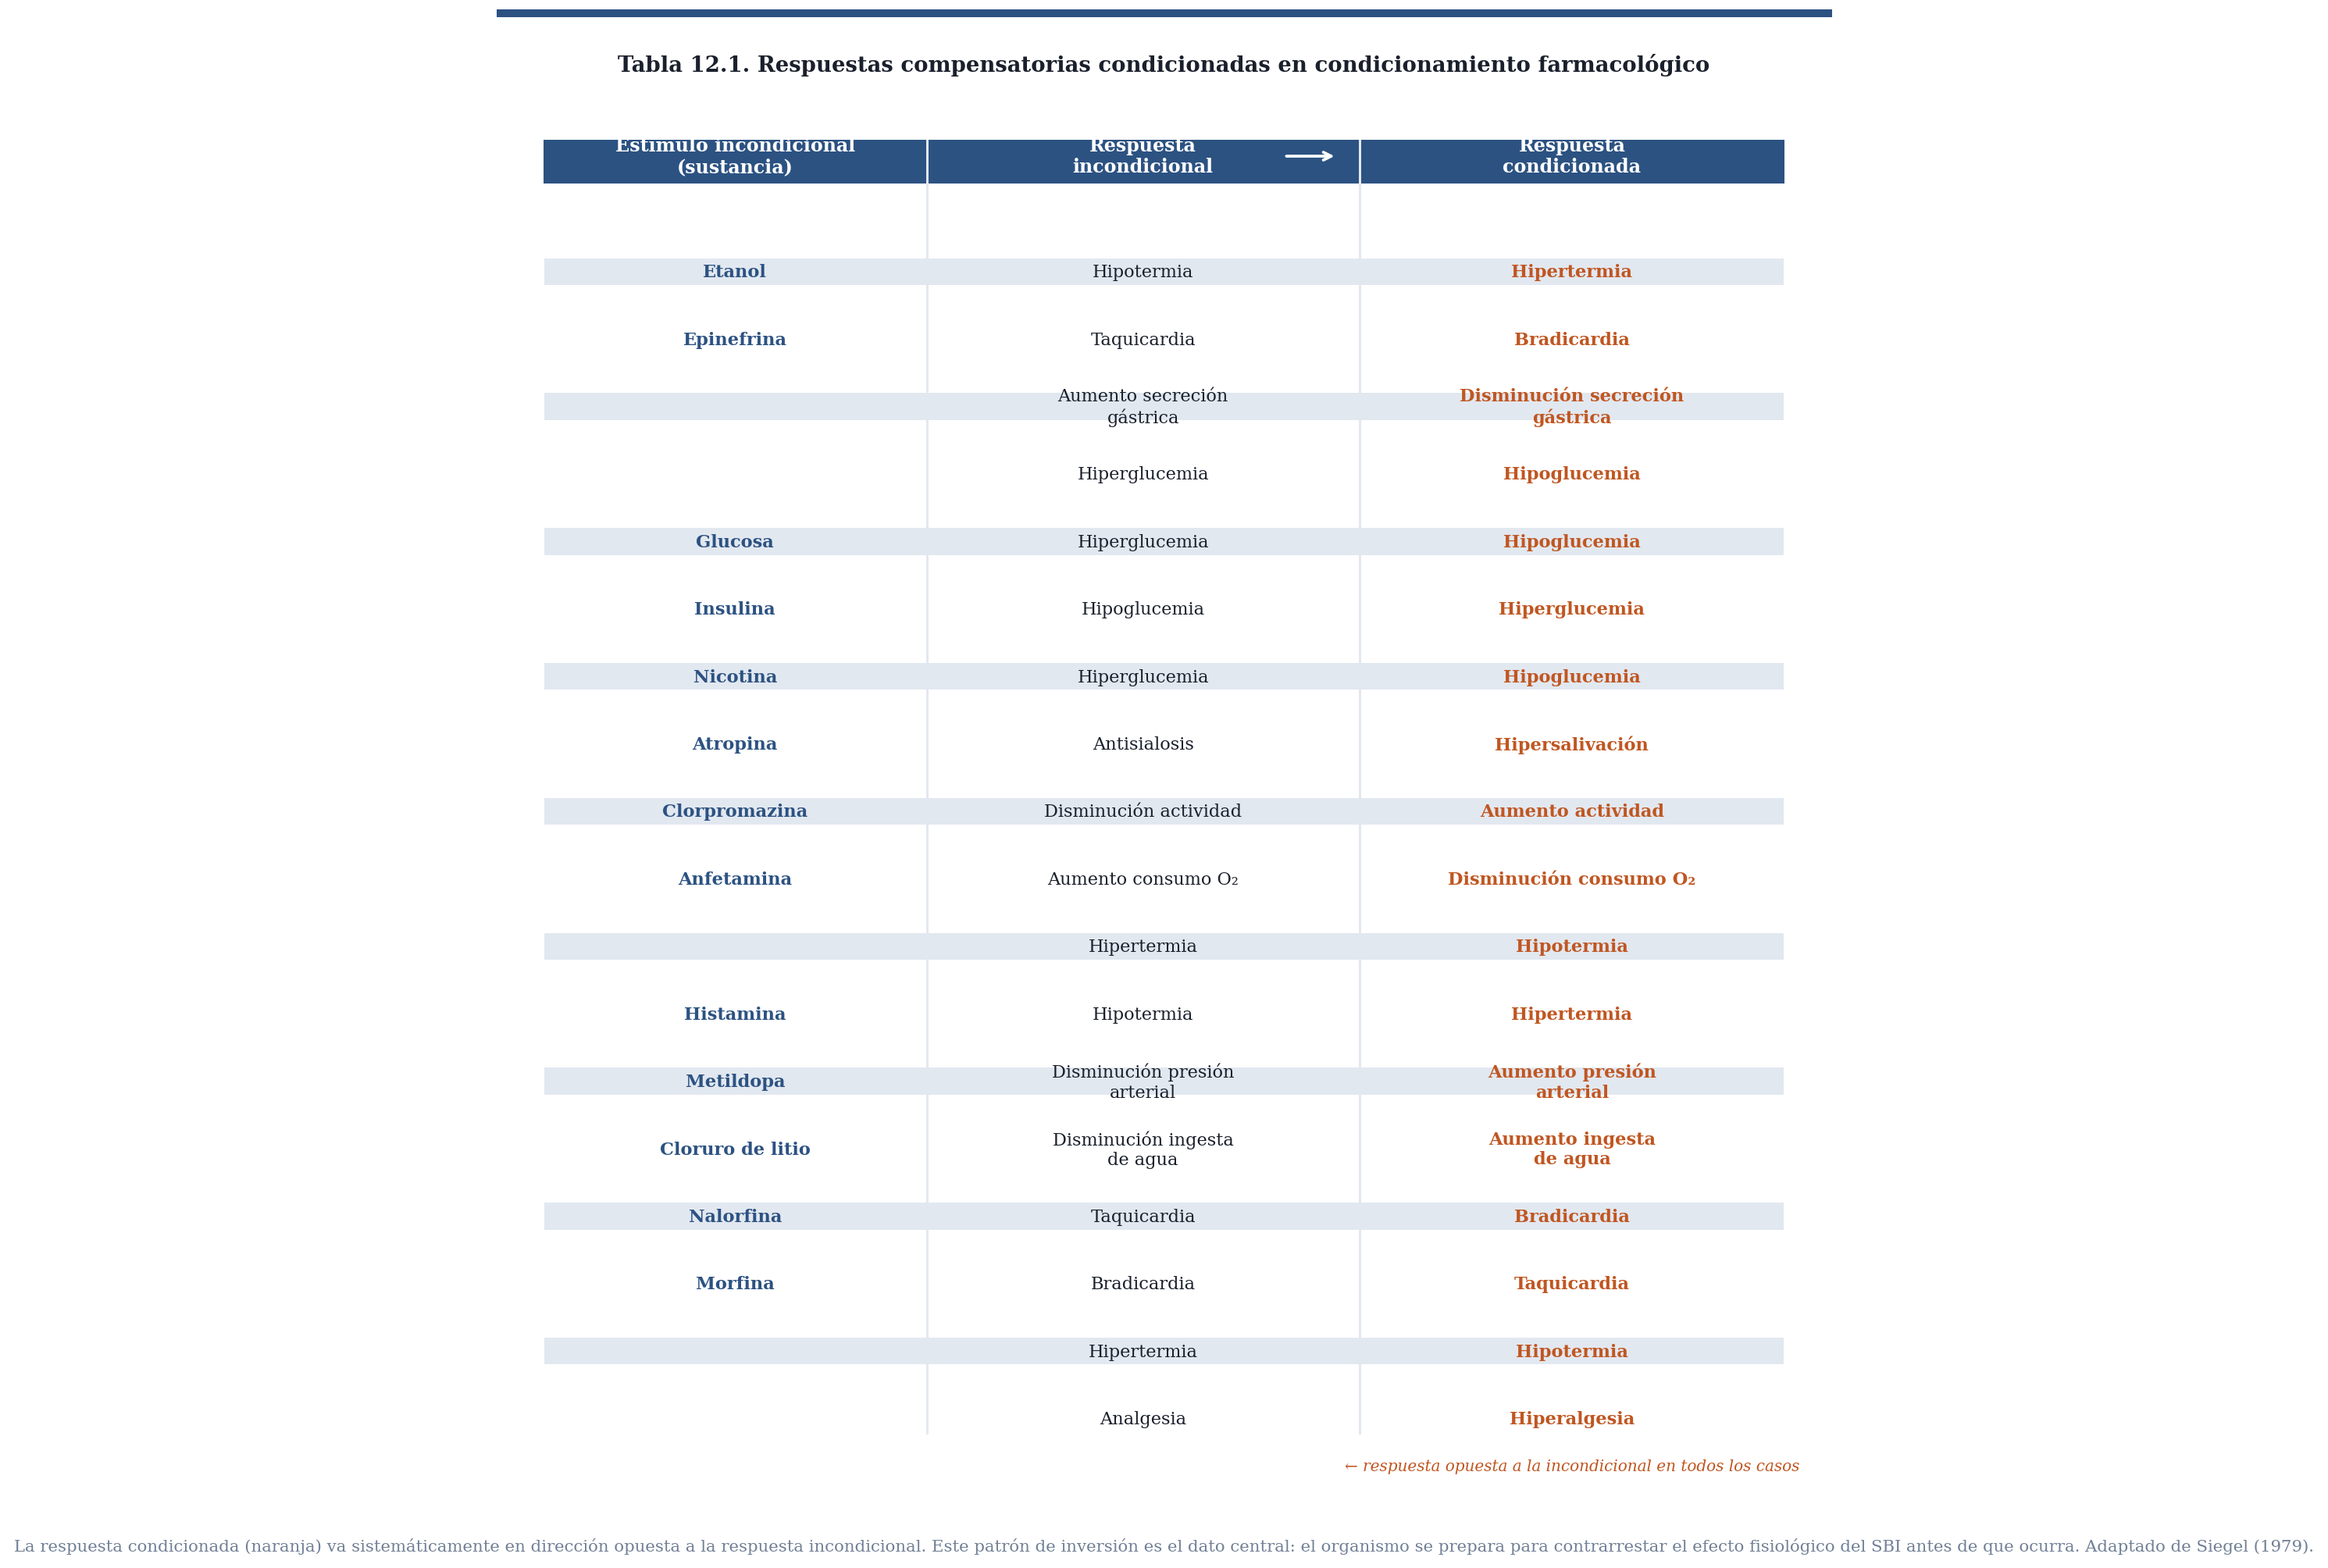
\includegraphics[keepaspectratio]{Figuras/tabla_12_1_siegel.png}}

}

\caption{tabla\_12\_1\_Respuestas compensatorias}

\end{figure}%

\begin{quote}
\textbf{Note}

\textbf{{[}Respuestas compensatorias condicionadas en condicionamiento
farmacológico. Tres columnas: estímulo incondicional (sustancia),
respuesta incondicional, respuesta condicionada. Incluye etanol
(hipotermia → hipertermia), epinefrina (taquicardia → bradicardia),
morfina (analgesia → hiperalgesia), insulina (hipoglucemia →
hiperglucemia), entre otros casos. Adaptado de Siegel, 1979. El patrón
sistemático de inversión es el dato central.{]}}
\end{quote}

Siegel interpretó este patrón como \emph{respuestas compensatorias}: el
organismo se prepara para contrarrestar el efecto fisiológico del SBI
antes de que ocurra. El mecanismo, propuso, subyace a los fenómenos de
tolerancia a las drogas: con el uso repetido, el predictor contextual
(el ambiente donde se consume, el ritual de preparación) evoca
respuestas compensatorias que amortiguan el efecto de la droga,
requiriendo dosis crecientes para obtener el mismo efecto. La
consecuencia clínica más dramática es la sobredosis por
descontextualización: un adicto que recae en un entorno diferente al
habitual no activa las respuestas compensatorias típicas, y una dosis
que sería tolerable en el contexto habitual puede ser letal.

Estos resultados cerraron la puerta a la sustitución de estímulos como
principio general. La pregunta se desplazó: si la respuesta no es una
copia del reflejo, ¿qué principio determina qué conducta se observa ante
un predictor?

\mbox{}%
\section{3. La forma de la respuesta depende de lo que se anticipa y de
cómo se
anuncia}\label{la-forma-de-la-respuesta-depende-de-lo-que-se-anticipa-y-de-cuxf3mo-se-anuncia}

Que la respuesta al predictor no sea una copia del reflejo no significa
que sea arbitraria. Jenkins y Moore expusieron palomas a un
procedimiento en el que la iluminación de una tecla por unos segundos
era seguida por acceso a un SBI: comida para unas, agua para otras.
Fotografiaron las respuestas de las palomas en el momento del contacto
con la tecla. Cuando el SBI era agua, la respuesta era similar a la de
beber: el pico se insertaba lentamente y la garganta mostraba
movimientos de deglución. Cuando el SBI era comida, el pico golpeaba la
tecla con movimientos secos y rápidos, como al comer. Mismo predictor,
misma ubicación espacial, topografías funcionalmente distintas según lo
que anuncian.

\mbox{}%
\subsection{\texorpdfstring{\faIcon{video} Video: Respuestas para comida
y
agua}{ Video: Respuestas para comida y agua}}\label{b58fc729-690b-4000-b19f-365a4093b2ff7b7b3c20666120766964656f203e7d7d-video-respuestas-para-comida-y-agua}

Este clip muestra las respuestas de palomas ante una tecla iluminada
predictora de agua (izquierda) versus predictora de comida (derecha),
tomadas en el momento del contacto.

▶ \textbf{Ver video:}
\href{https://www.youtube.com/watch?v=50EmqiYC9Xw}{Respuestas para
predictores de comida y agua}

El mismo principio opera cuando distintos tipos de señales anuncian el
mismo SBI. Peter Holland presentó a ratas cuatro estímulos ---dos luces
y dos tonos--- todos seguidos de comida. Ante los tonos, las ratas
mostraban sacudidas de cabeza y sobresalto. Ante la luz localizada, se
paraban sobre sus patas traseras y se orientaban al comedero. Ante la
luz difusa, la conducta dirigida al comedero era predominante desde el
inicio. Topografías completamente distintas, misma consecuencia
anticipada. La forma de la respuesta condicionada no estaba determinada
solo por el SBI ni solo por el predictor, sino por la combinación de
ambos filtrada por la biología del organismo.

\begin{figure}[H]

{\centering 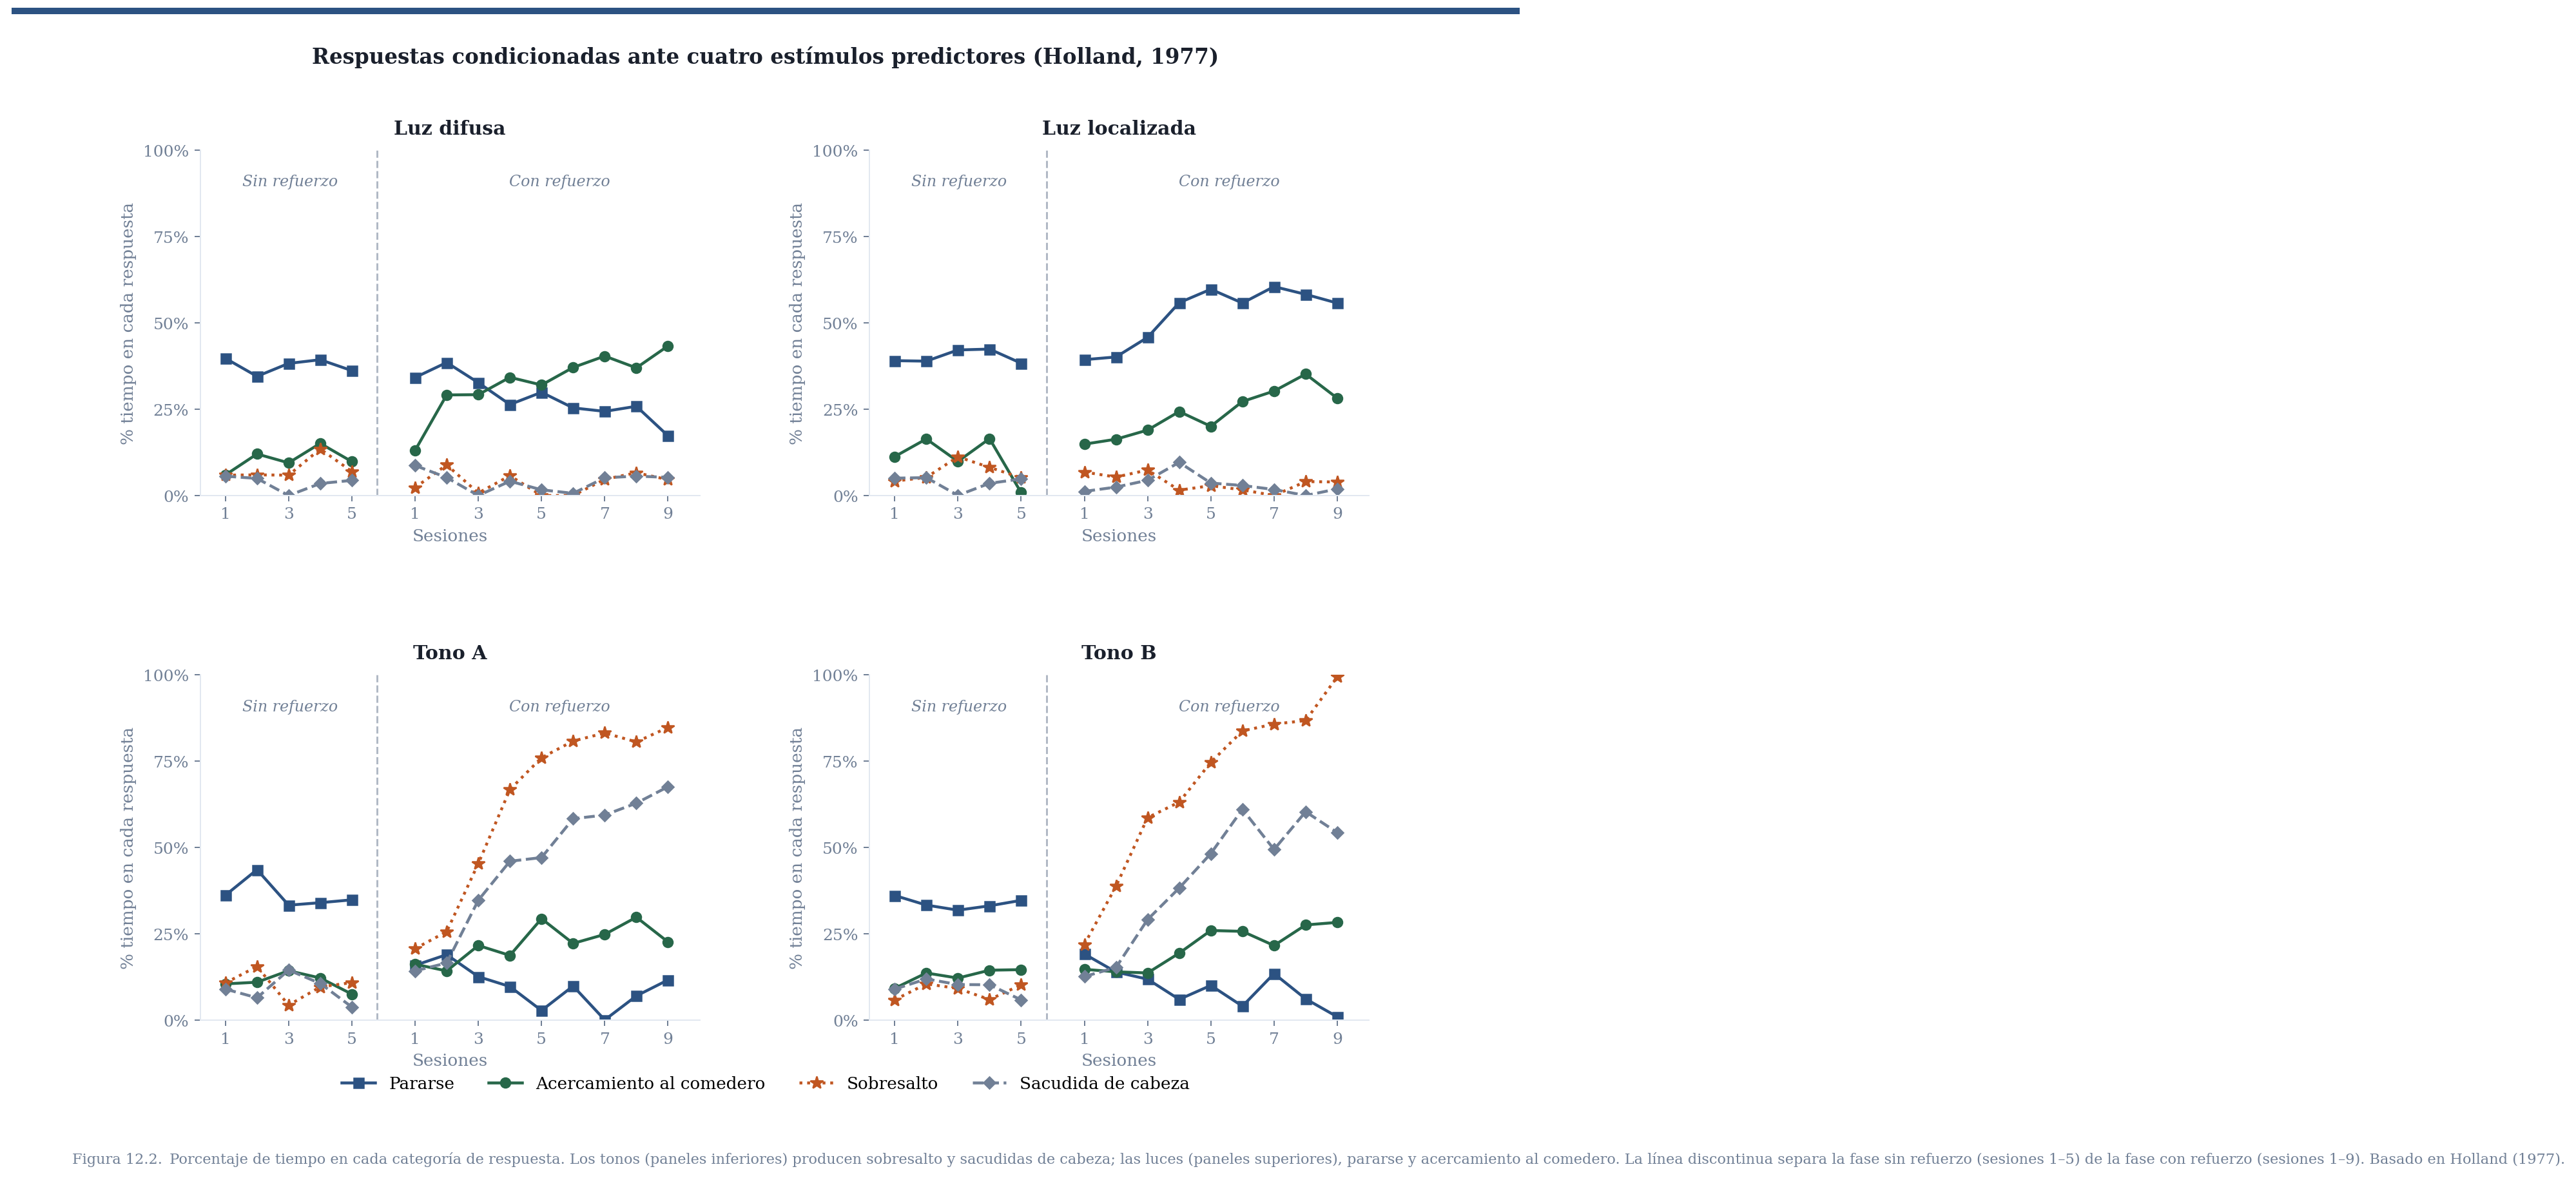
\includegraphics[width=7.8125in,height=\textheight,keepaspectratio]{Figuras/fig_12_2_holland.png}

}

\caption{Fig 1 Holland cuatro estímulos}

\end{figure}%

\begin{quote}
\textbf{Note}

\textbf{{[}Resultados de Holland (1977). Cuatro paneles, uno por cada
tipo de estímulo (luz difusa, luz localizada, tono A, tono B). Eje
horizontal: sesiones de condicionamiento. Eje vertical: porcentaje de
tiempo en cada tipo de respuesta. Las líneas representan: pararse (■),
acercamiento al comedero (●), sobresalto (★), sacudida de cabeza (○). En
los paneles de tono, sobresalto y sacudida de cabeza dominan; en los de
luz, pararse y acercamiento al comedero. El patrón se establece
rápidamente y persiste.{]}}
\end{quote}

Un resultado adicional del trabajo de Holland merece atención porque
establece algo sobre la naturaleza del aprendizaje subyacente. Una luz
ya establecida como predictora de comida bloqueó la adquisición de valor
predictivo de un tono presentado simultáneamente con ella en una segunda
fase de entrenamiento --- el efecto de bloqueo que vimos en el capítulo
sobre Rescorla y Wagner. Lo relevante aquí es que la luz nunca había
evocado las sacudidas de cabeza características de los tonos: sus
respuestas condicionadas eran completamente distintas en topografía.
Pero la \emph{información} que portaba sobre el SBI era idéntica. El
bloqueo ocurrió porque lo que se aprende es información sobre la
estructura causal del entorno, no una asociación entre un estímulo y una
forma particular de respuesta. Las diversas topografías que observamos
son traducciones de esa información a través de los sistemas de
comportamiento del organismo, tema al que volveremos más adelante.

\mbox{}%
\section{4. El predictor en el flujo
conductual}\label{el-predictor-en-el-flujo-conductual}

Hasta aquí, el estudio de la traducción del conocimiento en acción había
ocurrido en condiciones algo artificiales: organismos inmovilizados o en
un vacío conductual, donde la única pregunta posible era qué respuesta
específica evocaba el predictor. Pero los organismos reales no esperan
pasivos a que llegue el siguiente estímulo. Están en movimiento
constante: buscando alimento, explorando, descansando, interactuando
socialmente. Es en ese flujo conductual donde los predictores aparecen y
donde su efecto debe analizarse.

A principios de la década de 1940, William Estes y B. F. Skinner
introdujeron un paradigma que desplazó la pregunta en esa dirección. Su
diseño constaba de dos fases. Primero, entrenaron a ratas a apretar una
palanca para obtener comida, hasta que respondieran a una tasa estable.
Luego, intercalado con esa conducta en curso, presentaron ocasionalmente
un tono durante unos segundos que terminaba con una descarga eléctrica.
Durante la presencia del tono las ratas dejaban de apretar la palanca,
retomando su tasa habitual una vez que el tono terminaba. El efecto no
era una nueva respuesta evocada sino una reorganización del
comportamiento ya en marcha: lo que Estes y Skinner llamaron
\emph{supresión condicionada} o respuesta emocional condicionada.

El ejemplo cotidiano más cercano lo conocemos bien quienes vivimos en la
Ciudad de México: cuando suena una alarma sísmica, la conducta que uno
estuviera realizando ---escribir, cocinar, hablar por teléfono--- se
interrumpe y se reorganiza en torno a la amenaza anticipada. Al terminar
la alerta, el comportamiento previo se retoma. Ese es exactamente el
patrón que Estes y Skinner documentaron en el laboratorio.

Años más tarde, Rescorla y Solomon extendieron el paradigma
sistemáticamente, combinando respuestas instrumentales mantenidas por
SBI positivos o negativos con estímulos predictores de SBI positivos o
negativos. Su análisis mostró que el efecto del predictor sobre la
conducta en curso no depende solo de la valencia del predictor, sino de
la \emph{interacción algebraica} entre el estado motivacional que
sustenta la respuesta instrumental y el que evoca el estímulo
condicionado. Un predictor de eventos aversivos suprime una respuesta
mantenida por comida, pero puede facilitar una respuesta de escape o
evitación. Un predictor de comida facilita una respuesta de
aproximación, pero podría interferir con una conducta de evitación. Un
EC inhibitorio ---señal de ausencia del SBI--- opera en dirección
contraria a un EC excitatorio, funcionando como señal de seguridad que
modula la conducta instrumental a la inversa.

\begin{figure}[H]

{\centering \pandocbounded{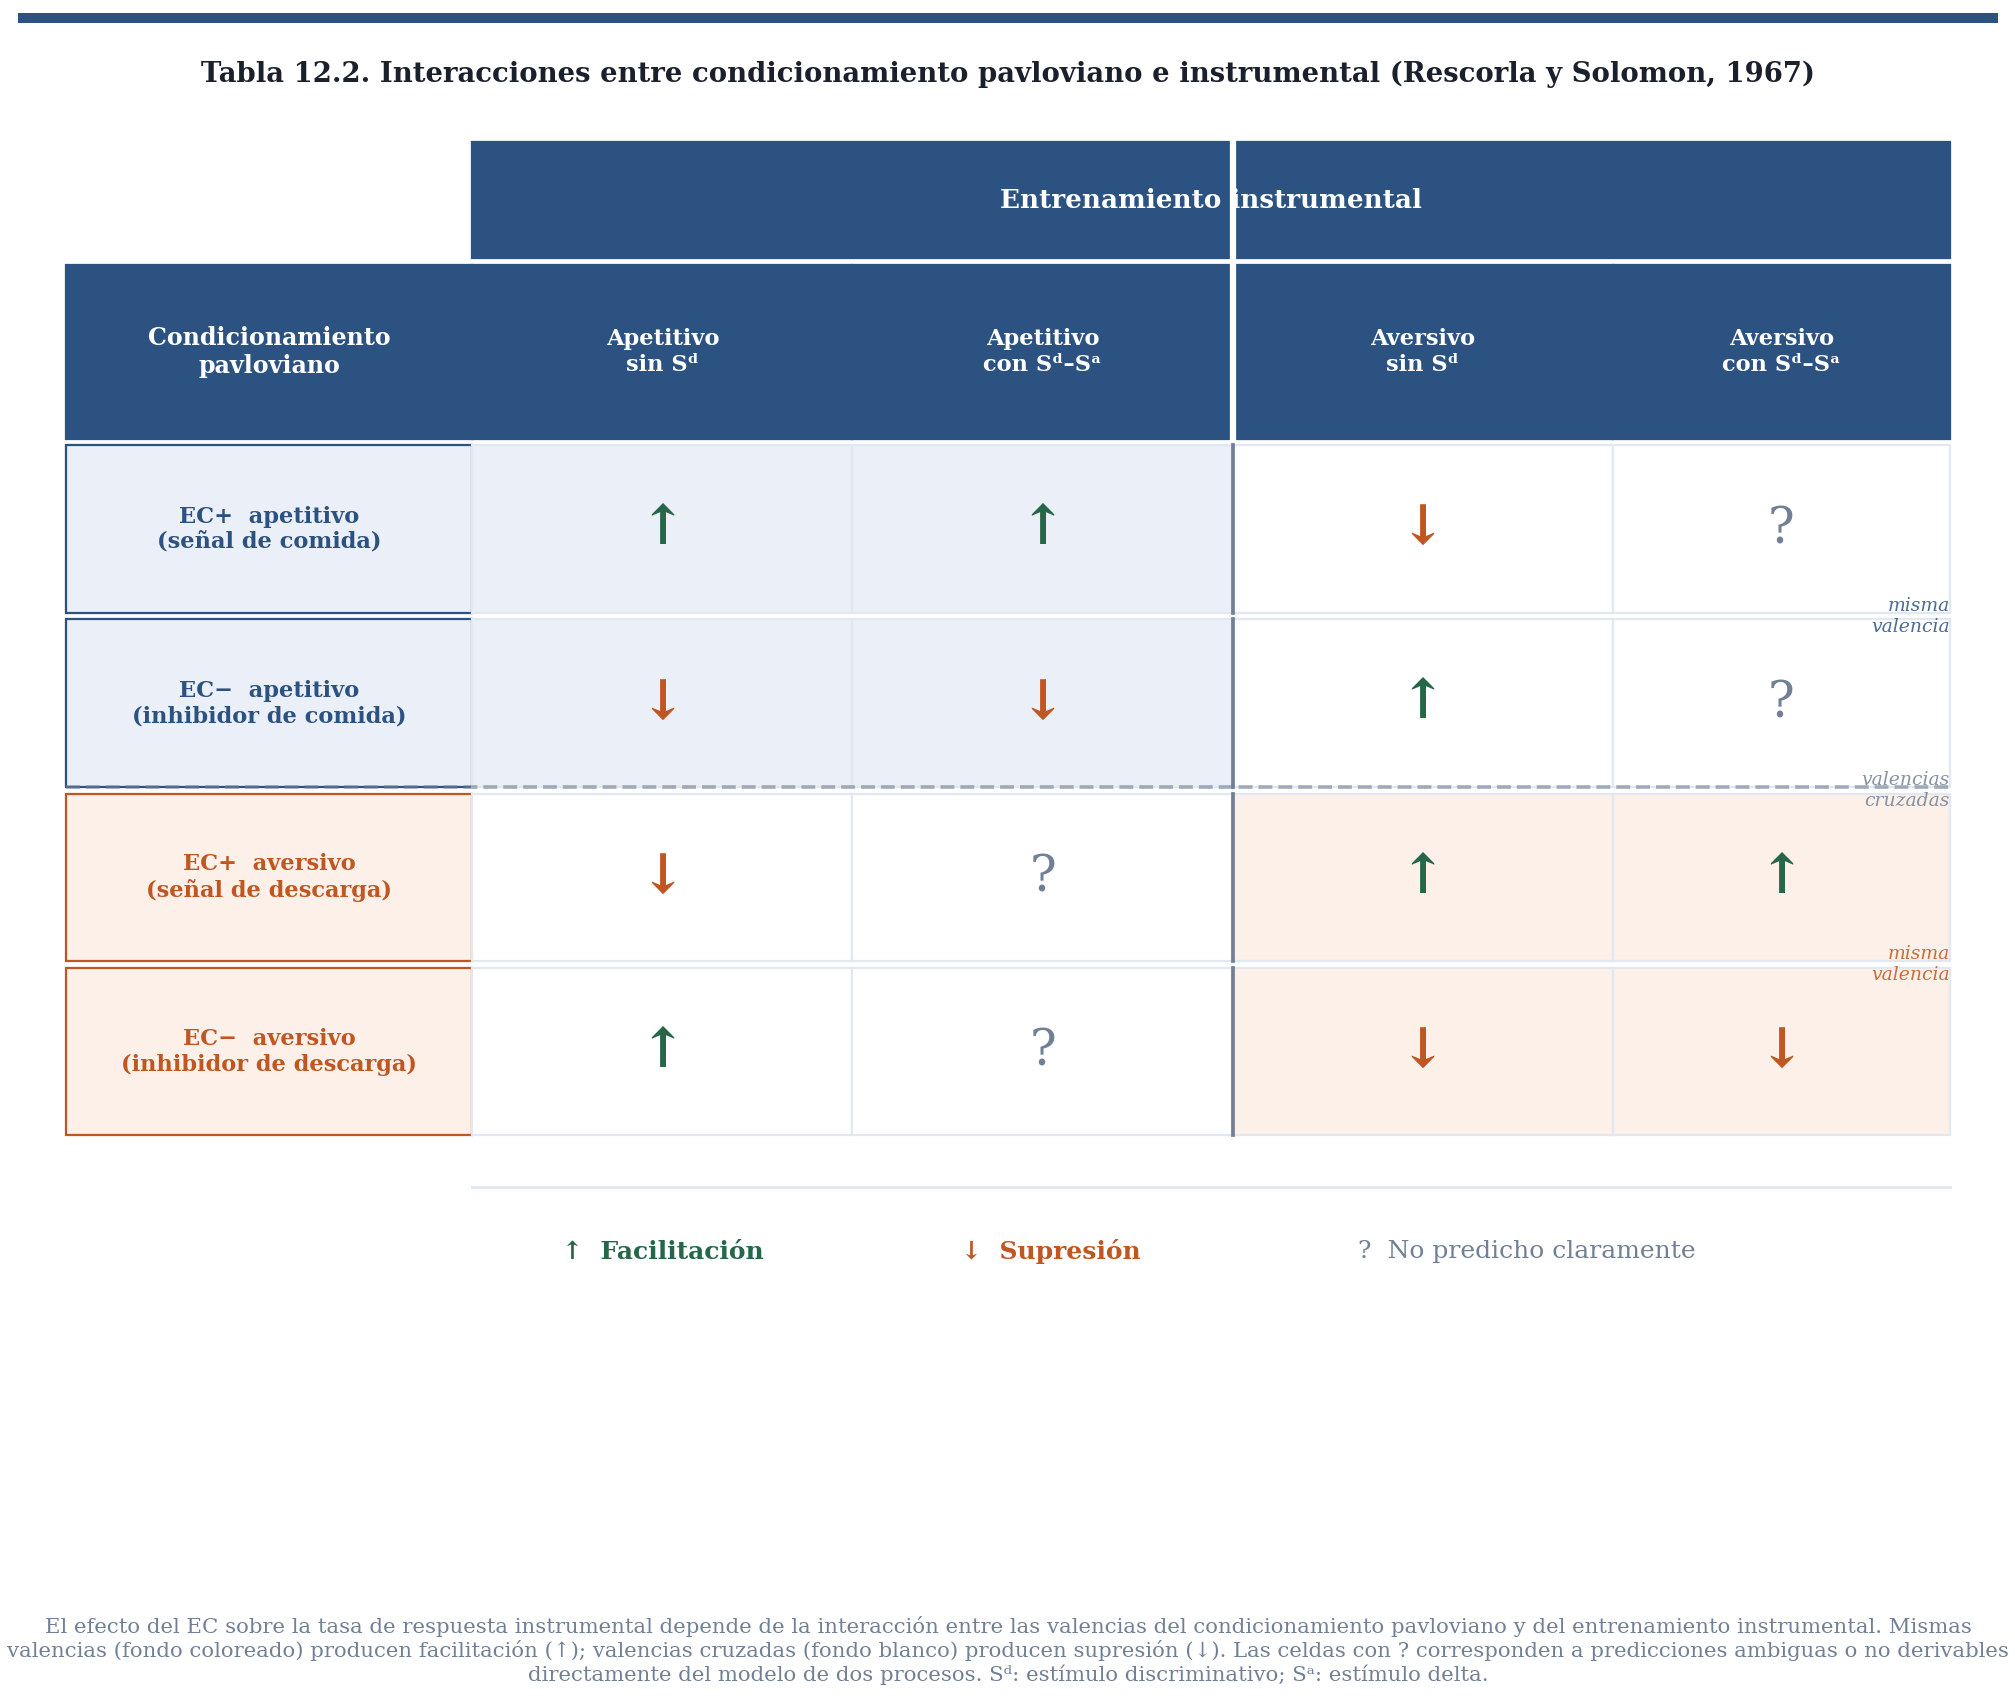
\includegraphics[keepaspectratio]{Figuras/tabla_12_2_rescorla_solomon.png}}

}

\caption{tabla\_12\_2\_Rescorla y Solomon}

\end{figure}%

\begin{quote}
\textbf{Note}

\textbf{{[}Combinaciones de procedimientos pavlovianos e instrumentales
según Rescorla y Solomon (1967). Filas: tipo de condicionamiento
pavloviano (EC+ apetitivo, EC-- apetitivo, EC+ aversivo, EC-- aversivo).
Columnas: tipo de entrenamiento instrumental y contexto (apetitivo sin
Sd, apetitivo con Sd--Sa, aversivo sin Sd, aversivo con Sd--Sa). Celdas:
dirección predicha del efecto sobre la tasa de respuesta instrumental (↑
facilitación, ↓ supresión, ? no predicho claramente). Las interacciones
mismas valencias producen facilitación; las valencias cruzadas producen
supresión.{]}}
\end{quote}

El predictor no actúa sobre una respuesta específica: actúa sobre el
estado motivacional del organismo, y ese estado interactúa con la
conducta en curso. El efecto conductual es el producto de esa
interacción.

\mbox{}%
\section{5. Predictores que adquieren valor
hedónico}\label{predictores-que-adquieren-valor-heduxf3nico}

Los efectos descritos hasta aquí ---respuestas compensatorias,
topografías condicionadas, modulación de conducta instrumental--- son
efectos sobre el \emph{comportamiento manifiesto}. Hay otro efecto,
menos visible pero igualmente fundamental: los predictores pueden
adquirir el valor afectivo del suceso biológicamente importante que
anuncian. No simplemente se comportan de manera orientada a la meta; el
predictor mismo comienza a gustar o a disgustar.

Pensemos en qué aprenden un niño y un pollo recién nacido sobre qué
cosas del mundo son comestibles. Algunos alimentos son apetecibles por
razones innatas. Pero para muchos otros, el valor hedónico es
completamente aprendido. Aprendemos a comer brócoli, a beber café, a
disfrutar del chile picante --- experiencias que en el primer contacto
pueden ser desagradables y que adquieren valor positivo gradualmente. Un
pollo recién nacido tiene que aprender a distinguir gusanos de piedras y
de excremento; todos tienen la textura y el tamaño aproximados de un
objeto comedible, pero solo uno tiene valor nutritivo. La pregunta es
cómo se forma esa preferencia.

Los experimentos de John García sobre aversión condicionada al sabor
ofrecen un modelo. En sus estudios clásicos, ratas bebían agua con sabor
a sacarina y horas después recibían una inyección que producía malestar
gastrointestinal. Una sola experiencia bastaba para que las ratas
rechazaran en el futuro el agua con ese sabor, aun cuando la sacarina en
sí es inocua. Lo que se había adquirido no era solo una respuesta de
evitación: era una nueva propiedad afectiva del estímulo. El sabor que
antes era neutro o agradable había adquirido valor hedónico negativo ---
se volvió repugnante. Las ratas no simplemente \emph{evitaban} la
sacarina; mostraban activamente señales de aversión al probarla, como si
fuera algo intrínsecamente desagradable.

El proceso opera simétricamente en la dirección positiva. Estímulos
repetidamente asociados con SBIs apetitivos adquieren valor hedónico
positivo. La visión del logo de una cadena de restaurantes favorita
puede producir un placer anticipatorio real, no solo la activación de
una conducta dirigida hacia él.

Esta capacidad de los predictores para adquirir valor hedónico tiene una
consecuencia importante para el estudio del aprendizaje de preferencias
en sentido amplio. Parte de lo que llamamos gustos, preferencias
estéticas y aversiones no son propiedades innatas de los objetos sino
propiedades aprendidas a través de la historia de asociaciones con SBIs.
La traducción del conocimiento en acción incluye, por lo tanto, no solo
la reorganización del comportamiento observable sino la restructuración
del valor afectivo del mundo.

\mbox{}%
\section{6. Predictores como imanes y
repelentes}\label{predictores-como-imanes-y-repelentes}

Si los predictores adquieren valor hedónico, cabe esperar que también
orienten espacialmente al organismo hacia o desde la fuente de
predicción. Brown y Jenkins describieron este efecto en palomas sin
entrenamiento previo en picar teclas. En su procedimiento, una tecla se
iluminaba durante unos segundos y al apagarse quedaba disponible acceso
a comida en el comedero, independientemente de lo que la paloma hiciera
durante la presentación del estímulo. Las palomas no necesitaban picar
la tecla: bastaba con ir al comedero cuando se apagara la luz. Sin
embargo, después de unas pocas presentaciones, las palomas comenzaban a
picar regularmente la tecla iluminada. Brown y Jenkins llamaron a este
resultado \emph{automoldeamiento}: la respuesta de picar la tecla
aparecía sin entrenamiento explícito, impulsada por la relación
predictiva entre el estímulo y el SBI.

\mbox{}%
\subsection{\texorpdfstring{\faIcon{video} Video: Automoldeamiento de la
respuesta de picar una
tecla}{ Video: Automoldeamiento de la respuesta de picar una tecla}}\label{b58fc729-690b-4000-b19f-365a4093b2ff7b7b3c20666120766964656f203e7d7d-video-automoldeamiento-de-la-respuesta-de-picar-una-tecla}

Este clip muestra las respuestas de palomas ante una tecla iluminada
predictora de agua (izquierda) versus predictora de comida (derecha),
tomadas en el momento del contacto.

▶ \textbf{Ver video:}
\href{https://www.youtube.com/watch?v=cacwAvgg8EA}{Respuestas para
predictores de comida y agua}

Una objeción natural es que las palomas quizás picaban porque,
ocasionalmente, sus picotazos precedían al acceso a comida ---
condicionamiento supersticioso, en el sentido que describió Skinner.
Para descartar esa posibilidad, Williams y Williams modificaron el
procedimiento de una manera decisiva: si la paloma picaba la tecla
iluminada, la comida \emph{no} se entregaba en ese ensayo. Solo cuando
la paloma no picaba obtenía el acceso al SBI. Este es el
\emph{procedimiento de omisión}: responder ante el predictor tiene un
costo directo y real en términos de obtención del SBI. Si el picotazo
fuera mantenido por sus consecuencias, el procedimiento de omisión
debería eliminarlo rápidamente. No lo hizo: las palomas continuaron
picando la tecla incluso cuando eso les costaba la comida.

\textbf{{[}FIGURA 12.3: Comparación esquemática de los procedimientos de
automoldeamiento estándar y de omisión. Dos paneles superiores muestran
la contingencia en cada procedimiento: en el estándar, picar la tecla es
independiente de la comida; en el de omisión, picar la tecla previene la
comida. Panel inferior: tasa de respuesta de picar la tecla a lo largo
de sesiones en ambas condiciones. En el procedimiento de omisión la tasa
se reduce parcialmente pero persiste muy por encima de cero, demostrando
que la respuesta no está mantenida por sus consecuencias positivas.
Basado en Williams y Williams (1969).{]}}

El resultado revela que la orientación hacia el predictor no está
gobernada por las consecuencias de las respuestas dirigidas a él. Está
gobernada por la relación predictiva entre el estímulo y el SBI: el
predictor actúa como un imán que atrae el comportamiento del organismo
hacia él, independientemente de si ese acercamiento resulta adaptativo
en un contexto particular. La imagen del imán captura algo real: el
acercamiento hacia predictores de SBIs apetitivos y el alejamiento ante
predictores de SBIs aversivos o ante predictores de la \emph{ausencia}
de un SBI positivo son efectos simétricos del mismo principio. El
estímulo que anuncia algo biológicamente relevante adquiere \emph{valor
hedónico o de incentivo} que orienta espacialmente la conducta --- un
fenómeno que la literatura denomina motivación de incentivo.

Esta propiedad opera fundamentalmente sobre predictores localizables. Un
estímulo difuso --- un cambio de iluminación general en el ambiente ---
no produce el mismo efecto de atracción que un estímulo puntual en el
espacio. Cuando el predictor no tiene una ubicación definida, el
organismo no puede orientarse hacia él, y el efecto de imán se
transforma en conducta dirigida al sitio donde el SBI suele aparecer ---
como en los experimentos de Holland donde la luz difusa producía
principalmente conducta de acercamiento al comedero.

\mbox{}%
\section{7. Sistemas de
comportamiento}\label{sistemas-de-comportamiento}

Los resultados acumulados en este capítulo dibujan una imagen del
organismo radicalmente diferente de la que asumía la teoría del reflejo:
no un sistema que espera estímulos para reaccionar, sino un agente en
movimiento constante, organizado funcionalmente en torno a metas
biológicamente importantes, que ante un estímulo predictor reorganiza su
conducta de maneras específicas y sensibles al contexto. William
Timberlake y Jerry Hogan formularon el marco teórico que integra esta
visión con la biología evolutiva de cada especie.

Su propuesta es que el comportamiento puede describirse como
\emph{sistemas funcionales} organizados por la historia evolutiva y las
exigencias del nicho ecológico. Cada sistema está ligado a una tarea
adaptativa ---alimentación, depredación, defensa, reproducción,
interacción social--- y se descompone en subsistemas, modos
motivacionales, módulos y patrones de acción organizados
jerárquicamente. El sistema de alimentación de una rata carnívora, por
ejemplo, incluye un subsistema de depredación. Ese subsistema lleva al
organismo a diferentes \emph{modos} según la situación: búsqueda general
cuando la comida no está a la vista, búsqueda focalizada cuando hay
indicios de proximidad, y manipulación-consumo cuando el alimento ya
está presente. Dentro de cada modo, \emph{módulos} específicos integran
filtros perceptuales y programas motores apropiados para el entorno
particular: rastrear, perseguir, inmovilizar, manipular, ingerir.

\textbf{{[}FIGURA 12.4: Representación jerárquica del sistema de
depredación de la rata (subsistema del sistema de alimentación). Cuatro
columnas: Subsistema (Depredación), Modo (Búsqueda general / Búsqueda
focalizada / Manipulación-consumo), Módulo (Viajar, Perseguir, Capturar,
Probar, Ingerir, Rechazar, Acaparar) y Acción (Locomoción/Exploración,
Rastrear/Cortar, Atrapar/Morder, Gnaw/Sostener, Masticar/Tragar,
Escupir/Limpiar, Cargar). Las flechas muestran cómo los estímulos en
cada nivel activan módulos y acciones específicas. Adaptado de
Timberlake (1994).{]}}

En este marco, el impacto de un estímulo predictor depende de dónde
encaja en la jerarquía. Una señal temporal y difusa de la proximidad de
una presa activa el modo de búsqueda general. Una señal localizada
activa la búsqueda focalizada y el organismo se orienta y aproxima. Una
señal que indica que el alimento ya está disponible para manipulación
activa el modo de consumo. El predictor no produce una respuesta fija:
posiciona al organismo en un punto de la jerarquía conductual, y desde
ahí la conducta sigue su curso natural guiada por las propiedades de los
estímulos disponibles.

Tres experimentos ilustran cómo el sistema de comportamiento de la
especie filtra y transforma el significado del predictor.

En el primero, Timberlake usó un pequeño balín metálico rodante como
señal que predecía la entrega de comida en ratas. Las ratas
interactuaban intensamente con el balín: lo perseguían, lo atrapaban, lo
transportaban y lo mordisqueaban. El movimiento del balín activaba los
filtros perceptuales del módulo de captura predatoria, evocando
comportamientos funcionalmente idénticos a los de caza. Timberlake
encontró además una disociación que revela la estructura jerárquica:
cuando el intervalo entre el balín y la comida era de 7.6 segundos, la
rata lo perseguía activamente (modo de búsqueda focalizada); cuando el
intervalo se reducía a 2.6 segundos, la rata abandonaba el balín y se
dirigía directamente al comedero (transición al modo de
manipulación-consumo). El mismo estímulo activa modos diferentes según
su posición temporal relativa al SBI.

En el segundo experimento, Timberlake y Grant usaron a una rata viva,
sujeta a una plataforma, como estímulo predictor de comida para la rata
sujeto. Las ratas sujeto no intentaban morder ni comer a la rata-señal.
Como forrajeadoras sociales que en condiciones naturales siguen a
congéneres para encontrar alimento, la señal activó el módulo social del
sistema de alimentación. Las ratas sujeto mostraron comportamientos de
contacto social: olfateo, acicalamiento y trepar sobre la rata-señal ---
respuestas completamente distintas a las que producía un bloque de
madera de tamaño similar, ante el cual solo mostraban orientación sin
ninguna interacción social. Las ratas tratan a la rata-señal como lo que
es: una fuente de información sobre comida que tiene valor hedónico, no
como comida en sí. Y así fue --- pero la respuesta de información social
era exactamente la apropiada para una especie que forrajea en grupo.

El tercer experimento subraya que los sistemas de comportamiento son
específicos a la especie. Los hámsteres son roedores solitarios que
compiten por el alimento. Cuando Timberlake repitió el experimento
usando a otro hámster como señal de comida, el resultado fue opuesto: la
señal inhibió el acercamiento, activando probablemente un módulo de
competencia o defensa. Misma lógica experimental, misma relación
predictor-SBI, conducta radicalmente distinta porque la biología
evolutiva de la especie es diferente.

Lo que los tres experimentos tienen en común es que el organismo no
responde al predictor como si fuera la meta final. Lo procesa a través
de su biología y su historia de aprendizaje, y activa la secuencia
conductual que corresponde a ese predictor en ese sistema funcional
particular. El condicionamiento clásico, desde esta perspectiva, no
genera respuestas nuevas: modula los patrones de comportamiento
preorganizados que la especie ya posee y las secuencias previamente
aprendidas por el organismo a lo largo de su historia individual.

\mbox{}%
\section{8. La ventaja adaptativa de
anticipar}\label{la-ventaja-adaptativa-de-anticipar}

Después de recorrer la evidencia presentada en este capítulo, queda una
pregunta de orden más general. Aun si aceptamos que los estímulos
predictores producen respuestas compensatorias, adquieren valor
hedónico, atraen o repelen, modulan conducta en curso y activan sistemas
organizados de comportamiento, debemos preguntar si todo ello representa
una ventaja adaptativa en condiciones ecológicas reales, más allá del
laboratorio. Karen Hollis abordó esta cuestión directamente.

En experimentos con peces territoriales, condicionó a machos a
anticipar, mediante un estímulo predictor, dos tipos de encuentros
biológicamente importantes. Cuando el predictor anunciaba la llegada de
un macho rival, los machos condicionados lograban defender su territorio
de manera más efectiva: se posicionaban de manera más agresiva y
lograban una ventaja clara en los combates. Cuando el predictor
anunciaba la llegada de una hembra receptiva, los machos condicionados
mostraban algo difícil de lograr en su especie: atenuaban su agresividad
territorial inicial ---que suele ser un obstáculo para el
apareamiento--- cortejaban con mayor rapidez y, crucialmente, producían
significativamente más crías que los machos no condicionados.

La señal no solo reorganizaba el comportamiento de manera inmediata:
cambiaba el resultado reproductivo de los organismos. El valor de la
predicción no reside solo en conocer mejor la estructura del entorno,
sino en posicionar al organismo conductualmente antes de que el evento
llegue, cuando todavía hay tiempo de prepararse.

Estos resultados enlazan directamente con el argumento que abre el
libro: la selección natural opera a través del éxito del comportamiento
en la solución de problemas adaptativos. El condicionamiento clásico
habrá evolucionado ---y se habrá mantenido en linajes tan distantes como
peces, ratas y humanos--- porque anticipar un suceso biológicamente
importante antes de que ocurra otorga una ventaja real en la competencia
por recursos, territorios y parejas.

\mbox{}%
\section{Conclusión}\label{conclusiuxf3n-1}

Este capítulo cierra el módulo sobre asignación de crédito. La historia
que hemos contado en este bloque va del problema ---cómo aprender qué
predice qué--- hasta el mecanismo formal ---el error de predicción como
señal de actualización--- y termina aquí, con la pregunta de qué hace el
organismo con lo que aprendió.

La respuesta no es simple ni uniforme. Aprender a predecir un suceso
biológicamente importante transforma al organismo en al menos cuatro
dimensiones: cambia las respuestas fisiológicas que preparan al
organismo para el evento (respuestas compensatorias); cambia el valor
afectivo de los estímulos del entorno (adquisición de valor hedónico);
activa secuencias motoras orientadas hacia o desde el predictor
(motivación de incentivo); y reorganiza el comportamiento en curso en
función del estado motivacional evocado (modulación instrumental). La
forma específica que adoptan estos cambios depende de la naturaleza del
SBI anticipado, de las propiedades del predictor, de los sistemas
funcionales propios de la especie, y de las posibilidades de acción que
el entorno físico ofrece --- lo que la literatura llama
\emph{affordances}: un predictor de comida en un comedero localizado
produce conducta de acercamiento solo si el espacio lo permite; el mismo
predictor en un entorno sin posibilidades de aproximación producirá otro
patrón de reorganización. No hay una respuesta condicionada: hay una
reorganización condicionada.

El siguiente módulo desplazará el foco de los predictores a las
acciones: de los estímulos que anuncian SBIs a las respuestas que los
producen, y de ahí a los principios que gobiernan cómo los organismos
distribuyen su comportamiento en el tiempo para obtener el mayor
beneficio posible dado su entorno. La pregunta será cuándo actuar, con
qué frecuencia, y bajo qué reglas de distribución del comportamiento.
Son preguntas que solo pueden formularse cuando el organismo tiene
control sobre la ocurrencia del SBI --- cuando puede producirlo, no solo
predecirlo.

\mbox{}%
\section{Conexiones}\label{conexiones-5}

\mbox{}%
\subsection{Hacia atrás}\label{hacia-atruxe1s}

Este capítulo es la consecuencia conductual de los capítulos de
asignación de crédito. Los capítulos 6 y 7 establecieron las condiciones
bajo las cuales los organismos aprenden a predecir SBIs a través de
estímulos y respuestas respectivamente. Los capítulos 8 y 11
formalizaron ese aprendizaje: Bush y Mosteller introdujeron el error de
predicción para eventos individuales; Rescorla y Wagner lo extendieron a
compuestos de estímulos, derivando formalmente el bloqueo. El bloqueo
por Holland que discutimos en la sección 3 es exactamente la misma
demostración empírica que el capítulo 11 explicó formalmente: la luz
bloquea al tono porque ya reduce el error de predicción a cero, no
porque sea contigua al SBI.

La sección sobre Estes y Skinner y Rescorla y Solomon (sección 4)
conecta el condicionamiento pavloviano con el instrumental, anticipando
el tema del siguiente módulo. Su análisis de estados motivacionales
cruzados es la primera vez en el libro que las dos formas de aprendizaje
--- predecir y producir --- aparecen en el mismo experimento.

\mbox{}%
\subsection{Hacia adelante}\label{hacia-adelante}

El módulo que sigue estudia el comportamiento instrumental: respuestas
que \emph{producen} SBIs en lugar de simplemente predecirlos. La
distinción entre comportamiento evocado (reflexivo, condicionado
clásicamente) y comportamiento emitido (operante, seleccionado por sus
consecuencias) que Skinner formuló es el punto de partida de ese módulo.
Este capítulo establece por qué esa distinción importa: los principios
que gobiernan la reorganización conductual ante predictores no son los
mismos que gobiernan la distribución del comportamiento emitido en el
tiempo. Ambos dependen de la historia de refuerzos, pero lo hacen de
maneras cualitativamente distintas.

El aprendizaje de preferencias discutido en la sección 5 reaparecerá en
el módulo sobre valor: cómo los SBIs adquieren valor y cómo ese valor
guía la distribución del comportamiento en situaciones de elección.

\mbox{}%
\section{Resumen}\label{resumen-6}

La teoría de sustitución de estímulos --- la primera propuesta sobre
cómo el aprendizaje se traduce en acción --- resultó insuficiente ante
la evidencia de respuestas compensatorias en dirección opuesta a la
respuesta incondicional. La forma de la respuesta ante el predictor
depende de la naturaleza del SBI anticipado (Jenkins y Moore) y del tipo
de señal disponible (Holland), no de la topografía del reflejo original.
Los estímulos predictores adquieren valor hedónico propio, subyaciendo
al aprendizaje de preferencias y aversiones. En el flujo conductual, los
predictores actúan como moduladores del estado motivacional del
organismo, con efectos de facilitación o supresión que dependen de la
interacción algebraica entre los estados motivacionales en juego (Estes,
Skinner, Rescorla y Solomon). Los predictores localizables adquieren
valor de incentivo que los convierte en imanes o repelentes espaciales:
el automoldeamiento y el procedimiento de omisión establecen que esta
atracción no está gobernada por las consecuencias de las respuestas
dirigidas al predictor. El modelo de sistemas de comportamiento de
Timberlake y Hogan integra estos resultados con la biología evolutiva:
los predictores modulan patrones de comportamiento preorganizados, y la
forma de esa modulación depende del sistema funcional y de la especie.
Los experimentos de Hollis demostraron que esta traducción del
conocimiento en acción produce ventajas adaptativas reales en términos
de éxito territorial y reproductivo.

\mbox{}%
\section{Ejercicios}\label{ejercicios-4}

\textbf{1.} Un paciente con dolor crónico recibe morfina regularmente en
el hospital, siempre en la misma habitación y con los mismos rituales
(enfermera, jeringa, olor del cuarto). Después de un tiempo, el médico
decide dar de alta al paciente y continuar la misma dosis en casa.
Usando la teoría de Siegel sobre respuestas compensatorias, ¿qué
predices sobre el efecto de la primera dosis en casa en comparación con
las dosis en el hospital? ¿Qué predicción hace esta teoría sobre la
probabilidad de sobredosis?

\textbf{2.} En el experimento de Jenkins y Moore, la forma de la
respuesta condicionada ante la tecla iluminada refleja la naturaleza del
SBI, no la topografía de la respuesta incondicional. Diseña un
experimento análogo usando una especie y un SBI de tu elección que
permita distinguir entre sustitución de estímulos y motivación de
incentivo como explicaciones de la respuesta condicionada. ¿Qué
resultados esperarías bajo cada predicción?

\textbf{3.} Rescorla y Solomon predicen que el efecto de un EC
excitatorio apetitivo sobre una respuesta instrumental depende del SBI
que mantiene esa respuesta. Un EC+ predictivo de comida se superpone a
dos grupos de ratas: uno cuya palanca-respuesta es reforzada con comida,
y otro cuya palanca-respuesta es reforzada con evitación de descarga
eléctrica. ¿Cuál es la predicción del modelo de estados motivacionales
para cada grupo? ¿Facilita o suprime el EC+ la respuesta de palanquear
en cada caso?

\textbf{4.} El procedimiento de omisión de Williams y Williams es
conceptualmente más poderoso que un diseño de control yoked para
descartar el condicionamiento supersticioso. Explica por qué. ¿Qué
explicación alternativa descarta el control yoked que el procedimiento
de omisión no descarta, y viceversa?

\textbf{5.} En el experimento del balín de Timberlake, el intervalo
entre la señal y la comida determinaba qué modo conductual se activaba:
búsqueda focalizada con 7.6 segundos, y transición a consumo con 2.6
segundos. ¿Qué implica este resultado sobre la representación temporal
que el organismo tiene del SBI anticipado? ¿Cómo distingues esta
explicación de la alternativa de que simplemente la respuesta más
reciente al SBI se refuerza con mayor probabilidad?

\textbf{6.} \emph{(Reflexión)} El modelo de sistemas de comportamiento
predice que la misma relación predictor-SBI puede producir respuestas
completamente distintas en especies diferentes. Identifica un caso de
comportamiento humano cotidiano donde puedas reconocer la huella de
sistemas funcionales preorganizados (alimentación, afiliación social,
defensa, reproducción) siendo modulados por predictores aprendidos. ¿Qué
tipo de evidencia te llevaría a preferir una explicación en términos de
sistemas de comportamiento sobre una explicación en términos de hábitos
aprendidos por refuerzo?

\mbox{}%
\section{Lecturas recomendadas}\label{lecturas-recomendadas-4}

\textbf{Siegel, S. (1983).} Classical conditioning, drug tolerance, and
drug dependence. En R. G. Smart et al.~(Eds.), \emph{Research advances
in alcohol and drug problems} (Vol. 7). Plenum. --- Presentación
accesible de la teoría de respuestas compensatorias con abundante
evidencia farmacológica. El punto de entrada más directo a la literatura
sobre tolerancia condicionada.

\textbf{Holland, P. C. (1977).} Conditioned stimulus as a determinant of
the form of the Pavlovian conditioned response. \emph{Journal of
Experimental Psychology: Animal Behavior Processes, 3}(1), 77--104. ---
El artículo original de Holland. Las secciones de método y resultados
son accesibles y las figuras son el referente estándar para ilustrar la
dependencia de la respuesta condicionada en el tipo de señal.

\textbf{Rescorla, R. A., \& Solomon, R. L. (1967).} Two-process learning
theory: Relationships between Pavlovian conditioning and instrumental
learning. \emph{Psychological Review, 74}(3), 151--182. --- El artículo
teórico que establece el marco de dos procesos e introduce el análisis
de interacciones motivacionales. Denso pero importante.

\textbf{Timberlake, W., \& Lucas, G. A. (1989).} Behavior systems and
learning: From misbehavior to general principles. En S. B. Klein \& R.
R. Mowrer (Eds.), \emph{Contemporary learning theories}. Erlbaum. --- La
presentación más completa del modelo de sistemas de comportamiento. Los
primeros dos tercios son accesibles para estudiantes de licenciatura con
el bagaje de este libro.

\textbf{Hollis, K. L. (1997).} Contemporary research on Pavlovian
conditioning: A ``new'' functional analysis. \emph{American
Psychologist, 52}(9), 956--965. --- Revisión accesible de la evidencia
sobre ventajas adaptativas del condicionamiento, escrita para audiencia
general. Buen punto de cierre después de leer el capítulo.

\textbf{Garcia, J., \& Koelling, R. A. (1966).} Relation of cue to
consequence in avoidance learning. \emph{Psychonomic Science, 4}(3),
123--124. --- El experimento original sobre aversión al sabor. Tres
páginas que cambiaron la concepción del condicionamiento clásico. Ya lo
conocen del capítulo de asignación de crédito a estímulos; vale la pena
releerlo ahora desde la perspectiva del valor hedónico adquirido.

\bookmarksetup{startatroot}

\mbox{}%
\chapter{La Ley del Efecto y los Programas de
Refuerzo}\label{la-ley-del-efecto-y-los-programas-de-refuerzo}

\mbox{}%
\section{Del Conocimiento a la
Acción}\label{del-conocimiento-a-la-acciuxf3n}

Los capítulos anteriores construyeron una maquinaria sofisticada para
resolver el problema de la predicción. A lo largo de los bloques de
asignación de crédito y modelos formales, nuestro agente adaptativo
adquirió la capacidad de detectar qué estímulos predicen sucesos
biológicamente importantes, qué respuestas los producen, y cuánto vale
cada predictor. El capítulo anterior mostró cómo ese conocimiento
predictivo se traduce en acción a través de los sistemas de
comportamiento: las predicciones activan patrones organizados de
respuesta cuya forma refleja la historia evolutiva de la especie. Cada
organismo llega a esta situación con una historia de aprendizaje que ha
moldeado el valor de sus respuestas y la fuerza de sus predicciones.

Pero hay un problema que esa maquinaria no resuelve. Un depredador sabe
que cierta estrategia de acecho produce presas, pero ¿con qué frecuencia
debe intentarlo? Un empleado sabe que escribir informes produce un
salario, pero ¿cuántos informes al mes? Un estudiante sabe que estudiar
mejora sus calificaciones, pero ¿cómo distribuir ese esfuerzo a lo largo
del semestre? En todos estos casos, el organismo ya posee el
conocimiento relevante --- lo que necesita es una regla para traducir
ese conocimiento en una \emph{distribución temporal de acciones}.
¿Cuánto de cada respuesta, cuándo, y a qué ritmo?

Este es el problema de la acción, y con él abrimos un nuevo bloque del
libro. Los capítulos anteriores preguntaban \emph{qué predice qué}. A
partir de ahora, la pregunta central es \emph{qué hacer dado lo que se
sabe}. La diferencia no es menor: mientras la predicción puede evaluarse
como correcta o incorrecta, la acción debe evaluarse en función de sus
consecuencias a lo largo del tiempo --- y esas consecuencias dependen de
reglas del entorno que el organismo debe descubrir y a las que debe
adaptarse.

Una observación empírica servirá como punto de partida. Piensen en las
diversas formas en que las consecuencias de nuestras acciones llegan a
nosotros. Un vendedor de coches gana una comisión por cada venta --- la
consecuencia depende del número de ventas cerradas. Un pescador arroja
su línea y espera; el pez llega cuando llega, independientemente de
cuántas veces el pescador sacuda la caña. Una persona que espera el
autobús en la Ciudad de México puede esperar dos minutos o veinte --- la
frecuencia del transporte es variable e impredecible. Un trabajador
asalariado recibe su pago cada quincena, haya trabajado mucho o poco. En
cada caso, la relación entre lo que el organismo hace y la consecuencia
que obtiene tiene una estructura diferente. Y esa estructura, como
veremos, moldea profundamente la forma en que el organismo distribuye su
comportamiento.

La contribución central de este capítulo es mostrar que una de las
regularidades más robustas en toda la psicología --- quizá \emph{la} más
robusta --- es que el mismo organismo, trabajando por el mismo
reforzador y con la misma motivación, exhibe patrones de respuesta
radicalmente distintos dependiendo de las reglas que gobiernan la
relación entre su comportamiento y sus consecuencias.

\mbox{}%
\section{De Thorndike a Skinner: una nueva unidad de
análisis}\label{de-thorndike-a-skinner-una-nueva-unidad-de-anuxe1lisis}

La ley del efecto de Thorndike, que introdujimos en el capítulo 7,
propone que las respuestas seguidas de consecuencias satisfactorias se
fortalecen. El modelo de Bush y Mosteller del capítulo 8 formalizó esa
idea como una ecuación de actualización:
\(Q_{t+1} = Q_t + \alpha(R_t - Q_t)\), donde el valor de la respuesta se
ajusta en cada ensayo según el error de predicción. Esa formulación
captura bien la \emph{adquisición} del comportamiento --- cómo un
organismo que no sabe nada aprende gradualmente qué respuestas producen
consecuencias.

Pero hay una limitación fundamental en el marco experimental de
Thorndike y sus sucesores. La caja de escape de Thorndike, el laberinto
en T, y el callejón de carrera comparten una propiedad: en cada ensayo,
el organismo solo puede emitir la respuesta exitosa una vez. El gato
escapa una vez por ensayo. La rata elige un brazo del laberinto una vez
por ensayo. Lo que se mide es la probabilidad de la respuesta dado ese
estímulo, o la latencia --- cuánto tarda el organismo en ejecutar una
respuesta cuya ocurrencia está determinada por el experimentador. La
pregunta sobre \emph{cuántas veces} y \emph{con qué distribución
temporal} responde el organismo no puede siquiera formularse en estos
protocolos.

B. F. Skinner (1938) transformó esta situación con dos innovaciones que
cambiaron la unidad de análisis del campo entero. La primera fue
conceptual: distinguir entre respuestas \emph{provocadas} --- aquellas
para las cuales puede identificarse un estímulo antecedente, como el
parpadeo ante un soplo --- y respuestas \emph{emitidas} --- aquellas que
el organismo produce libremente sin un estímulo discreto que las
desencadene. Piensen en las respuestas de revisar el teléfono, caminar
hacia la cocina, tener una conversación, fumar un cigarrillo: ninguna es
provocada por un estímulo puntual. Todas ocurren en un flujo continuo,
compitiendo entre sí por el tiempo del organismo. La segunda innovación
fue metodológica: proponer la \emph{tasa de respuesta} --- el número de
respuestas por unidad de tiempo --- como la medida fundamental de la
disposición del organismo a actuar. Si en una hora fumo cinco cigarros,
mi tasa de fumar es de cinco respuestas por hora. Si mañana fumo ocho,
la tasa aumentó. La tasa captura en una sola dimensión lo que los
protocolos de ensayos discretos no podían medir: la probabilidad de que
un organismo produzca espontáneamente una acción en cualquier momento
del tiempo.

Para observar esa tasa, Skinner diseñó un espacio experimental con un
dispositivo --- una palanca para ratas, una tecla iluminada para palomas
--- que el organismo podía operar libremente, tantas veces como
quisiera, a cualquier ritmo. Y para visualizar los patrones temporales
del comportamiento, inventó el \emph{registro acumulativo}: un registro
continuo donde el eje horizontal marca el tiempo y el eje vertical
acumula cada respuesta como un escalón. La pendiente de la línea
resultante \emph{es} la tasa de respuesta: pendiente pronunciada indica
tasa alta; pendiente plana indica pausa.

Con estas herramientas, la ley del efecto adquiere una formulación
nueva. En la versión de Thorndike, el efecto del refuerzo es seleccionar
qué respuesta se fortalece. En la versión de Skinner, el efecto del
refuerzo opera en dos niveles: primero, selecciona cuál de las
respuestas que preceden al reforzador es la que queda vinculada a él (el
problema del aprendizaje, que ya abordamos); segundo, determina la
\emph{tasa de ocurrencia} de esa respuesta seleccionada (el problema de
la acción, que es el tema de este capítulo y los siguientes). La ley se
expresa ahora como una función: \(R = f(r)\), donde \(R\) es la tasa de
respuesta y \(r\) es alguna medida del reforzamiento recibido. La forma
de esa función --- qué tan sensible es la tasa de respuesta a los
cambios en el reforzamiento --- será precisamente lo que necesitamos
entender.

Una nota terminológica. Hasta ahora hemos llamado ``sucesos
biológicamente importantes'' a las consecuencias que importan a los
organismos, y esa es la descripción correcta cuando el foco está en la
predicción. A partir de este capítulo, cuando esas consecuencias operen
modificando la tasa de respuesta de una acción, las llamaremos
\emph{reforzadores} --- el término estándar de la tradición operante. Un
reforzador es un SBI que sigue a una respuesta y modifica su
probabilidad futura de ocurrencia. El concepto es el mismo; cambia la
función que desempeña en el análisis.

\mbox{}%
\section{Entornos intermitentes: los programas de
refuerzo}\label{entornos-intermitentes-los-programas-de-refuerzo}

El mundo fuera del laboratorio rara vez entrega consecuencias de manera
continua. No todos los intentos de un depredador son exitosos: las
presas frecuentemente escapan. No todas las visitas de una abeja a una
flor terminan en acceso a néctar. No en todas las visitas a un mercado
se encuentran mandarinas. La compra de un billete de lotería rara vez
produce un premio. Un estudiante que levanta la mano en clase a veces
recibe atención del profesor y a veces no. Las consecuencias
biológicamente importantes son, en su inmensa mayoría, intermitentes.

Un protocolo experimental donde cada respuesta va seguida de refuerzo
puede ser útil para estudiar la adquisición de una respuesta, pero no
captura la riqueza de las posibles relaciones entre comportamiento y
consecuencias en los entornos naturales. Skinner reconoció esto
tempranamente --- en parte por razones económicas, y en parte por
accidente, dejó de reforzar cada respuesta --- y se percató de que las
reglas que determinan cuándo y cómo se entrega un reforzador producen
efectos profundos y reproducibles sobre el comportamiento. A esas reglas
las llamó \emph{programas de refuerzo}.

Los programas de refuerzo son formalizaciones de una propiedad
estadística del entorno: la regla que mapea acciones a consecuencias. En
la terminología de los sistemas de retroalimentación que introdujimos en
el capítulo 5, los programas describen la \emph{función del entorno} ---
la transformación que convierte el comportamiento del organismo en una
tasa de reforzamiento. La otra mitad del sistema es la \emph{función del
organismo}, \(R = f(r)\): la transformación que convierte la tasa de
reforzamiento en una tasa de respuesta. Las dos funciones operan
acopladas en un lazo cerrado, exactamente como en los sistemas de
retroalimentación que ya conocen.

Skinner identificó dos dimensiones fundamentales que definen las reglas
del entorno. La primera es si la disponibilidad del reforzador depende
del \emph{número de respuestas} emitidas o del \emph{tiempo
transcurrido} desde el último reforzador. Piensen en la diferencia entre
un vendedor que gana por comisión (cada venta cuenta) y un pescador que
espera a que el pez muerda (el tiempo es lo relevante). La segunda
dimensión es si el criterio --- sea el número de respuestas o el tiempo
--- es \emph{fijo} o \emph{variable} de una ocasión a otra. El salario
quincenal llega siempre cada quince días; la espera del autobús varía
impredeciblemente.

Al combinar las dos dimensiones se generan cuatro programas básicos. En
los \emph{programas de razón}, el reforzador depende del número de
respuestas: razón fija (RF) cuando ese número es constante, razón
variable (RV) cuando varía aleatoriamente alrededor de una media. En los
\emph{programas de intervalo}, la disponibilidad del reforzador depende
del tiempo transcurrido: intervalo fijo (IF) cuando el tiempo es
constante, intervalo variable (IV) cuando varía aleatoriamente. Un punto
crucial que conviene aclarar desde el inicio: en los programas de
intervalo, transcurrido el tiempo requerido, el reforzador no se entrega
automáticamente --- el organismo debe emitir una respuesta para
obtenerlo. El tiempo ``abre'' la oportunidad; la respuesta la ejecuta.
Esta distinción separa los programas de intervalo de los programas de
\emph{tiempo fijo}, donde el reforzador se entrega independientemente de
la respuesta --- un arreglo que es, en esencia, condicionamiento clásico
temporal.

\textbf{{[}FIGURA 13.1: Tabla-diagrama de los cuatro programas básicos
de refuerzo. Dos dimensiones: eje horizontal (criterio por número de
respuestas vs.~por tiempo), eje vertical (fijo vs.~variable). Cada celda
contiene el nombre del programa (RF, RV, IF, IV), un ejemplo cotidiano,
y una miniatura del registro acumulativo típico. Paleta del libro: azul
\#2C5282 para las líneas de registro, naranja \#C05621 para las marcas
de reforzador, gris \#718096 para los ejes y etiquetas.{]}}

\begin{center}\rule{0.5\linewidth}{0.5pt}\end{center}

\mbox{}%
\section{Los patrones: regularidades
sorprendentes}\label{los-patrones-regularidades-sorprendentes}

La figura 13.2 muestra los registros acumulativos estilizados que se
observan con cada programa, obtenidos después de un entrenamiento
extenso. Estos patrones representan una de las regularidades más
robustas en toda la ciencia del comportamiento. Se han replicado en
ratas, palomas, monos, peces, humanos adultos y niños, bajo contextos
experimentales enormemente diversos. Cuando se entiende la regla del
entorno, el patrón del comportamiento se vuelve predecible con notable
precisión.

\textbf{{[}FIGURA 13.2: Registros acumulativos idealizados para los
cuatro programas básicos. VR: pendiente alta y sostenida, sin pausas.
FR: pendiente alta con pausas planas después de cada reforzador. VI:
pendiente moderada y estable. FI: festoneo (scalloping) --- pausa
después del reforzador seguida de aceleración progresiva. Las marcas
diagonales sobre la línea indican la entrega del reforzador. Colores del
libro.{]}}

Lo primero que llama la atención es que los programas fijos --- tanto de
razón como de intervalo --- producen una \emph{pausa} inmediatamente
después de la obtención del reforzador. El organismo deja de responder
durante un período variable, y luego retoma la actividad. En los
programas de razón fija, después de la pausa el organismo responde a una
tasa alta y constante hasta completar el requisito. En los programas de
intervalo fijo, después de la pausa la tasa se va acelerando
gradualmente conforme se acerca el momento en que el reforzador estará
nuevamente disponible, produciendo el patrón curvilíneo llamado
\emph{festoneo} (\emph{scallop}).

Esa pausa post-reforzamiento es notable porque, a primera vista,
contradice la ley del efecto. Si el refuerzo fortalece la respuesta que
lo precede, la tasa más alta debería ocurrir \emph{justo después} del
reforzador, cuando el efecto del fortalecimiento es más reciente. Lo que
se observa es exactamente lo opuesto. La contradicción es instructiva:
obliga a preguntar qué está ocurriendo que la versión más simple de la
ley del efecto no captura.

La historia de ese patrón a lo largo del entrenamiento revela algo más.
La figura 13.3 muestra cómo evoluciona el patrón de respuesta bajo un
programa de intervalo fijo a lo largo de sesiones sucesivas.

\textbf{{[}FIGURA 13.3: Adquisición del patrón de intervalo fijo.
Registro acumulativo esquemático mostrando cuatro fases de
entrenamiento. Fase I: tasa alta y relativamente constante (lo que
predeciría la ley del efecto simple). Fase II: tasa alta inmediatamente
después del refuerzo, con pausas incipientes. Fase III: pausas más
pronunciadas, inicio de festoneo. Fase IV: festoneo maduro --- pausa
limpia después del reforzador, aceleración progresiva. Adaptado de
Ferster y Skinner, 1957. Colores del libro.{]}}

En las primeras sesiones, el patrón es exactamente lo que el modelo de
Bush y Mosteller del capítulo 8 predeciría: la tasa de respuesta es más
alta inmediatamente después del refuerzo, porque el valor \(Q\) de la
respuesta acaba de ser actualizado positivamente. Es solo después de
varias sesiones de entrenamiento --- cuando el organismo ha tenido
oportunidad de aprender la \emph{estructura temporal} del programa ---
que el patrón se invierte y aparece el festoneo maduro. Este dato tiene
dos implicaciones. La primera es que la ley del efecto simple no está
equivocada --- predice correctamente el comportamiento temprano. La
segunda es que algo adicional opera con el entrenamiento: el organismo
aprende a usar el reforzador como información temporal, no solo como
fortalecedor.

La otra regularidad central es la diferencia en tasas de respuesta entre
programas de razón y de intervalo. Los programas de razón variable
producen consistentemente tasas más altas que los de intervalo variable.
Esta diferencia podría parecer trivial --- quizá los animales en razón
variable simplemente reciben más reforzadores por unidad de tiempo, y la
tasa de respuesta más alta es consecuencia de esa diferencia en tasa de
reforzamiento. Para evaluar esta posibilidad, necesitamos un control
riguroso.

\mbox{}%
\section{El experimento de cajas
acopladas}\label{el-experimento-de-cajas-acopladas}

Catania (1971) diseñó un experimento ingenioso para descartar la
explicación por diferencia en tasas de reforzamiento. El arreglo,
conocido como \emph{protocolo de cajas acopladas} (\emph{yoked}),
funciona así: en una cámara, una paloma trabaja bajo un programa de
razón variable --- la tasa a la que responde determina su tasa de
reforzamiento y los intervalos entre reforzadores. En una segunda
cámara, otra paloma recibe un reforzador cada vez que la paloma líder lo
recibe. La segunda paloma solo necesita emitir una respuesta para
recogerlo, pero la \emph{disponibilidad} del reforzador depende
enteramente de lo que hace la primera. El resultado es que ambas palomas
experimentan exactamente la misma distribución temporal de reforzadores
--- la misma tasa de reforzamiento, los mismos intervalos entre
reforzadores. Lo único que difiere es la \emph{regla}: para la primera,
la tasa de reforzamiento depende proporcionalmente de su tasa de
respuesta; para la segunda, la tasa de reforzamiento es independiente de
su tasa de respuesta.

\textbf{{[}FIGURA 13.4: Registros acumulativos del experimento de cajas
acopladas (Catania, 1971). Panel superior: paloma bajo programa de razón
variable, tasa alta (\textasciitilde5 respuestas/segundo). Panel
inferior: paloma acoplada bajo programa de intervalo variable
resultante, tasa mucho menor (\textasciitilde1 respuesta/segundo). Ambas
reciben la misma tasa de reforzamiento. Las marcas de reforzador están
alineadas verticalmente para hacer visible la igualdad en la entrega de
refuerzos. Colores del libro.{]}}

El resultado es inequívoco: la paloma bajo razón variable responde a una
tasa aproximadamente cinco veces mayor que la paloma acoplada bajo
intervalo variable, a pesar de recibir exactamente la misma tasa de
reforzamiento. La tasa de reforzamiento no puede ser la explicación.
Algo en la \emph{estructura de la regla} --- en la forma de la función
de retroalimentación --- produce la diferencia.

¿Qué puede explicar este resultado? Se han propuesto dos mecanismos
complementarios, no mutuamente excluyentes. La distinción entre ellos
retoma una que ya encontramos en el capítulo 7: la perspectiva
\emph{molecular} analiza el comportamiento evento por evento --- qué
propiedades de cada respuesta individual son seleccionadas por el
refuerzo --- mientras que la perspectiva \emph{molar} analiza relaciones
agregadas entre tasas de respuesta y tasas de reforzamiento a lo largo
de períodos extendidos. La primera explicación opera en el nivel
molecular; la segunda en el molar.

\mbox{}%
\section{Primera explicación: el reforzamiento diferencial de tiempos
entre
respuestas}\label{primera-explicaciuxf3n-el-reforzamiento-diferencial-de-tiempos-entre-respuestas}

Hasta ahora hemos hablado de la respuesta como un evento puntual ---
presionar la palanca, picar la tecla. Pero cada respuesta tiene
propiedades adicionales que pueden ser objeto de selección por las
consecuencias. Un tirador de penaltis no solo patea: lo hace con cierta
fuerza, dirección y ángulo, y el resultado del tiro retroalimenta
selectivamente esas propiedades. Los porteros que bloquean más tiros del
lado derecho generan un sesgo en el tirador hacia el izquierdo. Las
propiedades de la respuesta --- no solo su ocurrencia --- son moldeadas
por el refuerzo.

Una propiedad especialmente relevante para los programas de refuerzo es
el \emph{tiempo entre respuestas} (TER): el intervalo temporal que
separa una respuesta de la siguiente. El recíproco de la tasa de
respuesta es precisamente el TER promedio: si respondo diez veces por
minuto, el TER promedio es de seis segundos. Pero los tiempos entre
respuestas no son uniformes. Los organismos responden en ráfagas ---
series rápidas de respuestas con TER cortos --- separadas por pausas con
TER largos. La distribución resultante está cargada hacia tiempos
cortos, porque las ráfagas contienen más respuestas que los intervalos
entre ellas.

Ahora viene el punto clave. En un programa de razón variable, cada
respuesta tiene la misma probabilidad de producir el reforzador --- una
en \(n\), donde \(n\) es el requisito promedio. Esa probabilidad no
depende de la duración del TER que precede a la respuesta: un TER corto
y uno largo tienen la misma chance de terminar en refuerzo. El programa
es \emph{neutro} respecto a la distribución de TER; la deja intacta. En
un programa de intervalo variable, la situación es diferente. El
reforzador se vuelve disponible después de que transcurre un tiempo, y
se entrega a la primera respuesta que ocurre después de ese momento.
Conforme pasa más tiempo desde la última respuesta, la probabilidad de
que un reforzador se haya acumulado y esté esperando \emph{crece}. Por
lo tanto, las respuestas precedidas por TER largos tienen una
probabilidad mayor de encontrar un reforzador disponible que las
respuestas precedidas por TER cortos. El programa termina reforzando
selectivamente los TER largos, lo cual desplaza la distribución de TER
hacia duraciones más altas, lo cual produce tasas de respuesta más
bajas. La asimetría entre los dos tipos de programa no es que uno
refuerce TER cortos y el otro TER largos: es que uno es neutro y el otro
sesga hacia TER largos.

La evidencia para esta explicación viene de dos fuentes. La primera es
descriptiva: en programas de intervalo variable, la distribución de TER
observados se asemeja efectivamente a la distribución de TER que fueron
seguidos por refuerzo. La segunda es experimental: es posible modificar
directamente la distribución de TER mediante programas diseñados para
reforzar selectivamente ciertos intervalos. Los \emph{programas de
reforzamiento diferencial de tasas bajas} (DRL, por sus siglas en
inglés) exigen que el organismo espere al menos cierto tiempo entre
respuestas --- digamos, 20 segundos --- para obtener el reforzador. Bajo
DRL, las palomas aprenden a responder con TER extraordinariamente
largos, produciendo tasas bajísimas. Simétricamente, los programas que
requieren TER menores a un cuarto de segundo producen tasas
extremadamente altas. El TER es una propiedad genuinamente reforzable
del comportamiento.

\begin{center}\rule{0.5\linewidth}{0.5pt}\end{center}

\mbox{}%
\section{Segunda explicación: sensibilidad a las
correlaciones}\label{segunda-explicaciuxf3n-sensibilidad-a-las-correlaciones}

La explicación por tiempos entre respuestas opera a nivel molecular ---
en la microestructura temporal de las respuestas individuales. La
segunda explicación opera a nivel molar --- en la relación agregada
entre tasas de respuesta y tasas de reforzamiento.

Recordemos la ley del efecto de Skinner: \(R = f(r)\). La tasa de
respuesta es una función de la tasa de reforzamiento. Pero la tasa de
reforzamiento no es un dato fijo del entorno --- es ella misma resultado
de la interacción entre el comportamiento del organismo y la regla del
programa. En un programa de razón variable RV-30, si el organismo
responde 30 veces por minuto obtiene un reforzador por minuto; si
responde 60 veces por minuto obtiene dos; si responde 120, obtiene
cuatro. La relación entre tasa de respuesta y tasa de reforzamiento es
\emph{proporcional} --- responder más rápido siempre produce más
reforzadores. En un programa de intervalo variable IV-60s, una vez que
el organismo responde con frecuencia suficiente para no ``perderse'' los
reforzadores disponibles, responder más rápido no produce ningún
reforzador adicional. La tasa máxima de reforzamiento está limitada por
el valor del intervalo y es insensible a incrementos en la tasa de
respuesta.

Para pensar en un ejemplo cotidiano: un traductor que cobra por
cuartilla traducida tiene una relación proporcional entre esfuerzo y
ganancia --- cada cuartilla adicional produce más dinero. Una persona
que espera el autobús tiene una relación diferente: una vez que está en
la parada, el número de veces que asoma la cabeza para ver si viene no
afecta cuándo llega.

La propuesta de Baum (1973) es que los organismos son sensibles a esta
correlación entre su tasa de respuesta y su tasa de reforzamiento. No
solo responden más cuando hay más refuerzo (eso es la ley del efecto
simple); responden más cuando responder más produce más refuerzo ---
cuando la correlación es positiva. Un organismo cuyo comportamiento está
controlado por esa correlación es una instancia del sistema de
retroalimentación que introdujimos en el capítulo 5. La tasa de
respuesta determina la tasa de reforzamiento, y esta a su vez determina
la tasa de respuesta, hasta que el sistema alcanza un equilibrio.

La figura 13.5 muestra las funciones de retroalimentación --- la
transformación que el programa hace de la tasa de respuesta del
organismo en una tasa de reforzamiento --- para programas de razón
variable y de intervalo variable.

\textbf{{[}FIGURA 13.5: Funciones de retroalimentación (función del
entorno). Eje horizontal: tasa de respuesta (R). Eje vertical: tasa de
reforzamiento (r). La función de RV es una recta desde el origen
(relación proporcional, pendiente = 1/n donde n es el requisito
promedio). Las funciones de IV son curvas cóncavas que se aceleran
rápidamente con tasas bajas y se estabilizan en una asíntota
(1/intervalo programado). Se muestran dos curvas de IV: una ``rica''
(intervalo corto, asíntota alta) y una ``pobre'' (intervalo largo,
asíntota baja). Una línea vertical punteada marca una tasa máxima de
respuesta. Azul para RV, verde para IV rico, gris para IV pobre, naranja
para la línea de tasa máxima. Colores del libro.{]}}

La forma de las funciones revela inmediatamente por qué los organismos
responden más bajo razón que bajo intervalo. En razón, cada respuesta
adicional acerca al organismo al siguiente reforzador --- invertir más
esfuerzo siempre rinde más. En intervalo, una vez alcanzada una tasa
moderada, el esfuerzo adicional es desperdiciado. Un organismo sensible
a estas correlaciones debería responder rápido bajo razón y
moderadamente bajo intervalo. Y eso es exactamente lo que se observa.

\begin{center}\rule{0.5\linewidth}{0.5pt}\end{center}

\mbox{}%
\section{El reforzador como estímulo
discriminativo}\label{el-reforzador-como-estuxedmulo-discriminativo}

Las dos explicaciones anteriores tratan al reforzador como una
consecuencia que modifica la probabilidad de la respuesta que lo precede
--- ya sea fortaleciendo ciertos TER o modulando la tasa de respuesta a
través de correlaciones. Pero el reforzador puede desempeñar un papel
adicional que no cabe en ninguna de esas dos funciones: actuar como una
\emph{señal} que predice las condiciones que vendrán a continuación.

Recuerden que en los capítulos de asignación de crédito vimos cómo los
organismos aprenden a usar estímulos del entorno como predictores de
sucesos biológicamente importantes. Skinner extendió esa lógica con un
movimiento que tiene la misma estructura que su innovación sobre las
respuestas. Así como liberó a la respuesta de necesitar un estímulo
provocador --- transformándola de evento discreto provocado en flujo
continuo de acción emitida, medida como tasa --- de la misma forma
liberó al estímulo de tener que provocar una respuesta discreta. En
lugar de un estímulo que elicita, Skinner propuso un estímulo que
\emph{dispone la ocasión}: un contexto en cuya presencia ciertas
respuestas producen reforzadores y otras no. Los llamó \emph{estímulos
discriminativos}. Su sala de estudio dispone la ocasión para
concentrarse; el bar dispone la ocasión para una cerveza. No son
estímulos que provocan respuestas como un reflejo --- son contextos que
informan al organismo sobre la regla respuesta-reforzador actualmente
vigente.

La idea potente de Skinner es que los propios reforzadores pueden
convertirse en estímulos discriminativos. Consideren un programa de
intervalo fijo de 60 segundos. Cada vez que el organismo obtiene un
reforzador, sabe algo: en los próximos 60 segundos, ninguna respuesta
producirá otro reforzador. El reforzador señala un período de ``sequía''
inminente. Un organismo que ha aprendido esta relación dejará de
responder inmediatamente después del reforzador --- no porque el
reforzamiento haya debilitado la respuesta, sino porque la ha informado.
La pausa post-reforzamiento en los programas fijos no es un fracaso de
la ley del efecto; es un éxito del aprendizaje discriminativo.

Piensen en un ejemplo de su vida cotidiana. Un examen parcial es, en
primera instancia, un reforzador (o un resultado aversivo, dependiendo
de la calificación). Pero también funciona como estímulo discriminativo:
les predice que la probabilidad de otro examen en los próximos días es
muy baja. El patrón de estudio que resulta --- alta intensidad antes del
examen, caída abrupta después --- tiene la misma forma que el festoneo
de las palomas bajo intervalo fijo. No es coincidencia: la estructura
temporal del programa es la misma.

Este análisis extiende de manera natural los principios del bloque
anterior. La asignación de crédito a estímulos, que estudiamos en el
capítulo 6, opera aquí sobre los propios reforzadores: el organismo
aprende qué señales --- incluyendo la ocurrencia misma del reforzador
--- predicen la disponibilidad de futuras oportunidades de
reforzamiento. La diferencia con el condicionamiento clásico es que lo
que se predice no es un suceso biológicamente importante sino una
\emph{relación respuesta-reforzador}: si esta respuesta, en este
momento, producirá o no una consecuencia.

\mbox{}%
\section{La función de retroalimentación:
formalización}\label{la-funciuxf3n-de-retroalimentaciuxf3n-formalizaciuxf3n}

Hasta ahora hemos descrito las funciones de retroalimentación
cualitativamente. Formalizar su forma precisa permite hacer predicciones
cuantitativas y revela algo sobre la estructura del problema.

Para los programas de razón, la formalización es inmediata. Si el
requisito promedio es \(n\) respuestas por reforzador, entonces la tasa
de reforzamiento \(r\) es directamente proporcional a la tasa de
respuesta \(R\):

\[r = \frac{R}{n}\]

Cada respuesta es una fracción \(1/n\) de un reforzador. La función es
una línea recta desde el origen con pendiente \(1/n\). Duplicar la tasa
de respuesta duplica la tasa de reforzamiento --- sin límite teórico.

Para los programas de intervalo, la formalización es más interesante. El
reforzador se programa cada \(t\) segundos en promedio, pero solo se
entrega cuando el organismo responde. Si el organismo responde a una
tasa lo suficientemente alta, no se ``pierde'' ningún reforzador
disponible y la tasa de reforzamiento se aproxima a \(1/t\). Si la tasa
de respuesta es muy baja, puede que el reforzador esté disponible pero
el organismo no responda a tiempo, y se pierdan oportunidades. La
función resultante es una curva cóncava que crece rápidamente con tasas
de respuesta bajas y se aplana conforme la tasa aumenta, acercándose
asintóticamente a \(1/t\).

Rachlin (1978) propuso una parametrización elegante que unifica ambos
tipos de programa en una sola expresión. (Staddon, 1979, y Prelec, 1982,
ofrecen derivaciones más rigurosas de la función de retroalimentación
para programas de intervalo, partiendo de supuestos diferentes sobre la
distribución de respuestas en el tiempo. Las tres formulaciones
coinciden en lo esencial: la función es cóncava y asintótica.
Presentamos la de Rachlin por ser la más accesible algebraicamente.)

\[r = d \cdot R^m\]

donde \(d\) es una constante de escala y \(m\) es un exponente entre 0 y
1 que captura el \emph{tipo} de función de retroalimentación. Cuando
\(m = 1\), la función es lineal --- un programa de razón. Conforme \(m\)
se acerca a 0, la función se aplana cada vez más, representando
programas donde la tasa de reforzamiento es cada vez más insensible a la
tasa de respuesta. En el límite, \(m = 0\) corresponde a un programa de
tiempo fijo, donde el reforzador llega independientemente del
comportamiento.

\textbf{{[}FIGURA 13.6: Familia de funciones de retroalimentación de
Rachlin. Eje horizontal: tasa de respuesta (R). Eje vertical: tasa de
reforzamiento (r). Cinco curvas para m = 1.0, 0.5, 0.2, 0.1, 0.05. La
curva con m = 1 es lineal (razón). Conforme m decrece, las curvas se
vuelven progresivamente más cóncavas. Todas parten del origen y
convergen en el mismo punto cuando R alcanza la tasa máxima. Etiqueta
para m = 1: ``RV''; etiqueta para m = 0.05: ``≈ Tiempo fijo''. Colores
del libro: azul para m = 1, gradiente hacia gris para m
decrecientes.{]}}

La expresión de Rachlin tiene una virtud adicional. Noten que el
recíproco de \(r\) es el tiempo entre reforzadores y el recíproco de
\(R\) es el tiempo entre respuestas. La ecuación puede leerse en
cualquiera de los dos marcos --- tasas o tiempos --- según convenga. En
capítulos posteriores, cuando formalicemos la \emph{función del
organismo} (\(R\) como función de \(r\)), el punto de equilibrio del
sistema será la intersección de las dos funciones: el punto donde lo que
el organismo produce (tasa de respuesta) es consistente con lo que el
entorno devuelve (tasa de reforzamiento).

\mbox{}%
\section{Lo que la ley del efecto simple no explica (y lo que
sí)}\label{lo-que-la-ley-del-efecto-simple-no-explica-y-lo-que-suxed}

Conviene hacer un balance. La ley del efecto en su versión más directa
--- las respuestas que preceden al refuerzo se fortalecen --- predice
correctamente varios aspectos de los datos: las tasas más altas bajo
razón que bajo intervalo (dado que en intervalo las respuestas lentas
son selectivamente reforzadas, mientras que en razón el programa es
neutro respecto a la velocidad), la relación positiva entre tasa de
refuerzo y tasa de respuesta, y el comportamiento temprano bajo
programas de intervalo fijo (tasa alta después del reforzador, antes de
que se desarrolle la discriminación temporal). Estos son logros del
modelo de Bush y Mosteller que ya conocen, aplicado ahora a la
distribución temporal de respuestas.

Pero la ley del efecto simple, sin principios adicionales, no explica la
pausa post-reforzamiento en los programas fijos (que requiere
aprendizaje discriminativo temporal), la forma específica del festoneo
en intervalo fijo (que requiere sensibilidad a la posición temporal
dentro del intervalo), ni la magnitud exacta de la diferencia entre
razón e intervalo cuando las tasas de reforzamiento están igualadas (que
requiere sensibilidad a las correlaciones o al reforzamiento diferencial
de TER).

Para inicios de los años 60, el panorama era el siguiente: la ley del
efecto de Thorndike, transformada y refinada por Skinner, había ampliado
su dominio desde la adquisición de respuestas individuales hasta el
mantenimiento del comportamiento en estado estable. Se había reconocido
que las reglas del entorno --- los programas de refuerzo --- determinan
no solo la tasa de respuesta sino su distribución temporal. Se había
descubierto que los propios reforzadores pueden actuar como señales
discriminativas. Y se había iniciado el análisis formal de los programas
como funciones de retroalimentación.

Pero dos resultados experimentales obtenidos al inicio de esa década
transformarían el campo. Herrnstein (1961) descubrió que cuando los
organismos pueden elegir entre dos respuestas que operan bajo programas
distintos, la \emph{proporción} de respuestas dedicadas a cada
alternativa iguala la proporción de reforzadores obtenidos --- una
regularidad cuantitativa notablemente precisa conocida como la \emph{ley
de igualación}. Este resultado desplazó la pregunta central del campo:
ya no se trataba de explicar la tasa de respuesta bajo un solo programa,
sino de explicar la \emph{distribución} del comportamiento entre
múltiples fuentes de reforzamiento que compiten por el tiempo del
organismo. La ley de igualación y sus extensiones son el tema del
siguiente capítulo.

\mbox{}%
\section{Conexiones}\label{conexiones-6}

\mbox{}%
\subsection{Hacia atrás}\label{hacia-atruxe1s-1}

\textbf{Sistemas de retroalimentación (capítulo 5).} La interacción
entre el organismo y los programas de refuerzo es un sistema de
retroalimentación de lazo cerrado: la tasa de respuesta determina, a
través de la función del entorno, la tasa de reforzamiento, y esta a su
vez determina, a través de la función del organismo, la tasa de
respuesta. La novedad respecto al capítulo 5 es que ahora tenemos una
taxonomía formal de las funciones del entorno --- los programas --- y
podemos parametrizar su forma (la expresión de Rachlin). Encontrar el
equilibrio del sistema requiere especificar ambas funciones y hallar su
intersección, que es lo que haremos en capítulos posteriores.

\textbf{Bush y Mosteller (capítulo 8).} La ley del efecto simple es el
modelo de Bush y Mosteller aplicado al valor \(Q\) de una respuesta:
\(Q\) sube cuando el refuerzo ocurre, baja cuando no, y se estabiliza
cuando la tasa de refuerzo es constante. Esa formulación genera dos
predicciones específicas para programas de refuerzo. La primera --- que
la tasa de respuesta debería ser proporcional a la tasa de refuerzo ---
es aproximadamente correcta para comparaciones dentro de un mismo tipo
de programa. La segunda --- que la tasa de respuesta debería ser máxima
inmediatamente después del reforzador --- es correcta durante las
primeras sesiones de entrenamiento bajo intervalo fijo, pero se invierte
con la experiencia. La inversión señala que un principio adicional
(aprendizaje discriminativo temporal) opera sobre la línea base que B\&M
establece.

\textbf{Rescorla-Wagner (capítulo 11).} La función discriminativa del
reforzador que explica las pausas en programas fijos es, en esencia, un
nuevo problema de asignación de crédito: el organismo aprende qué
señales predicen la disponibilidad del reforzador. El reforzador se
convierte en un estímulo discriminativo que predice la ausencia temporal
de oportunidades de reforzamiento. Los mismos principios de competencia
entre predictores --- que Rescorla-Wagner formaliza --- operan aquí
sobre la dimensión temporal.

\textbf{Traducción del conocimiento en acción (capítulo 12).} El
capítulo anterior mostró cómo los sistemas de comportamiento canalizan
las predicciones en acciones organizadas. Este capítulo complementa esa
perspectiva: las reglas del entorno moldean la \emph{distribución
temporal} de esas acciones. Los sistemas de comportamiento determinan la
\emph{forma} de la respuesta; los programas de refuerzo determinan su
\emph{frecuencia}.

\mbox{}%
\subsection{Hacia adelante}\label{hacia-adelante-1}

\textbf{La ley de igualación y la elección (capítulo siguiente).} La
diferencia entre razón e intervalo, aun con tasas de refuerzo igualadas,
deja abierta la pregunta de qué controla exactamente la distribución del
comportamiento cuando hay varias opciones disponibles simultáneamente.
Herrnstein (1961) descubrió que esa distribución obedece una regla
cuantitativa precisa --- la ley de igualación --- que reemplaza la tasa
absoluta de refuerzo por la tasa \emph{relativa} como variable
independiente. El paso de un programa a dos programas concurrentes
transforma el problema de la acción en un problema de elección.

\textbf{Maximización local.} Una vez establecida la regularidad de la
igualación, surge la pregunta de qué mecanismo la produce. Los modelos
de maximización local proponen que los organismos no necesitan calcular
proporciones globales: basta con que en cada momento elijan la
alternativa que ofrece la mayor probabilidad instantánea de refuerzo. El
mejoramiento (\emph{melioration}) y la maximización momentánea de Shimp
son dos versiones de esta idea, y ambas generan igualación como
resultado de equilibrio sin que el organismo ``sepa'' que está
igualando.

\textbf{Optimización en equilibrio.} Si tanto la función del organismo
como la función del entorno están especificadas, el estado estable del
sistema es su intersección --- el punto donde el organismo no tiene
incentivo para cambiar su tasa de respuesta. Staddon y Rachlin
formalizan esa perspectiva: la conducta en estado estable puede
entenderse como la solución de un problema de optimización sujeto a
restricciones. Esta perspectiva conecta los programas de refuerzo con
los modelos económicos de la elección y con la pregunta de si los
organismos maximizan alguna cantidad --- y si la igualación es o no una
consecuencia de esa maximización.

\textbf{La ley del efecto relativa.} El bloque cierra con una
formulación que juega un doble papel. Como regla de \emph{aprendizaje},
la ley del efecto relativa describe cómo se actualiza el valor de una
respuesta en función de las consecuencias obtenidas --- es una regla de
adquisición del conocimiento, análoga a Bush y Mosteller pero operando
sobre respuestas en contextos de elección. Como regla de \emph{acción},
describe cómo el organismo traduce esos valores en una distribución de
comportamiento --- una regla de respuesta que genera las proporciones
observadas en la igualación. Esa dualidad --- la misma ecuación leída
como algoritmo de aprendizaje y como función de elección --- es la
resolución formal del problema que abrió este bloque: la relación entre
lo que el organismo sabe y lo que hace.

\begin{center}\rule{0.5\linewidth}{0.5pt}\end{center}

\mbox{}%
\section{Resumen}\label{resumen-7}

Los organismos que han aprendido a predecir la estructura de su entorno
enfrentan un segundo problema: decidir qué hacer, cuánto y cuándo. El
estudio de este problema requirió un cambio en la unidad de análisis: de
respuestas discretas en ensayos controlados a la tasa de ocurrencia de
respuestas emitidas libremente a lo largo del tiempo. Skinner introdujo
tanto el concepto (la distinción entre respuestas provocadas y emitidas)
como la metodología (la cámara operante y el registro acumulativo) que
hicieron posible ese cambio.

Los entornos naturales no entregan consecuencias de manera continua.
Skinner formalizó las posibles reglas que relacionan acciones con
consecuencias como \emph{programas de refuerzo}, que varían en dos
dimensiones: si el criterio para obtener el reforzador es un número de
respuestas o un tiempo transcurrido, y si ese criterio es fijo o
variable. Los cuatro programas resultantes producen patrones de
respuesta distintos y extraordinariamente reproducibles, que constituyen
una de las regularidades empíricas más sólidas de la psicología.

Dos mecanismos complementarios contribuyen a explicar estos patrones. El
primero es el reforzamiento diferencial de tiempos entre respuestas: la
estructura del programa determina qué TER tienden a ser seguidos por
refuerzo, y esa propiedad de la respuesta es susceptible de selección
por sus consecuencias. El segundo es la sensibilidad a las correlaciones
entre tasas de respuesta y tasas de reforzamiento: los organismos
responden más cuando responder más produce más refuerzo. Los programas
de refuerzo pueden formalizarse como funciones de retroalimentación ---
la función del entorno en un sistema de lazo cerrado --- cuya forma
determina la estructura de la correlación entre comportamiento y
consecuencias.

La conclusión central del capítulo es que para entender el
comportamiento no basta con observar al organismo: es necesario
especificar con detalle las reglas que describen la relación entre
acciones y consecuencias, y formalizar esas reglas como propiedades del
entorno a las que el organismo debe adaptarse.

\begin{center}\rule{0.5\linewidth}{0.5pt}\end{center}

\mbox{}%
\section{Ejercicios}\label{ejercicios-5}

\textbf{1.} Un programa de razón fija RF-20 exige 20 respuestas por
reforzador. Un programa de intervalo fijo IF-60s entrega un reforzador
cada 60 segundos (más la primera respuesta después del intervalo). Supón
que un organismo responde a una tasa constante de 20 respuestas por
minuto bajo ambos programas. Calcula la tasa de reforzamiento que
obtendría en cada caso. ¿Cuál programa genera más reforzadores por
minuto a esa tasa de respuesta? ¿Qué pasaría si el organismo duplicara
su tasa de respuesta en cada programa?

\textbf{2.} Usa la función de retroalimentación de Rachlin,
\(r = d \cdot R^m\), con \(d = 0.1\). Calcula \(r\) para tasas de
respuesta de 10, 50 y 100 respuestas por minuto, con \(m = 1.0\)
(razón), \(m = 0.5\) y \(m = 0.1\) (intervalo). ¿A qué tasa de respuesta
la diferencia entre razón e intervalo se vuelve más pronunciada? ¿Qué
relación tiene esto con la forma de las funciones de retroalimentación?

\textbf{3.} En el capítulo 8 vimos que el modelo de Bush y Mosteller
predice que la tasa de respuesta más alta debería ocurrir inmediatamente
después del reforzador (porque \(Q\) acaba de ser actualizado
positivamente). Explica por qué esta predicción es correcta para las
primeras sesiones bajo intervalo fijo pero se invierte con el
entrenamiento extenso. ¿Qué principio adicional necesitas para explicar
la inversión?

\textbf{4.} Diseña un experimento (no necesita ser realizable, solo
conceptualmente claro) que permita distinguir entre la explicación por
TER y la explicación por correlaciones. Especifica qué programa usarías,
qué variable manipularías y qué resultado favorecería cada explicación.
(Pista: piensa en un programa que mantenga constante la correlación
entre tasa de respuesta y tasa de refuerzo pero altere la distribución
de TER reforzados.)

\textbf{5.} Imagina que un estudiante estudia bajo un programa de
``intervalo fijo'' natural: sus exámenes son cada tres semanas. Describe
el patrón de estudio que predecirías basándote en los datos de este
capítulo. Ahora imagina que el profesor cambia a exámenes sorpresa
(intervalo variable). ¿Cómo cambiaría el patrón? Explica tu predicción
en términos de la función discriminativa del examen como señal temporal.

\textbf{6.} \emph{(Reflexión)} Este capítulo presentó una regularidad
notable: el mismo organismo, con la misma motivación, produce patrones
de comportamiento radicalmente distintos bajo diferentes programas de
refuerzo. ¿Qué implica esto sobre dónde debemos buscar las causas del
comportamiento --- en las propiedades del organismo o en las propiedades
del entorno? Relaciona tu respuesta con la distinción entre la función
del organismo y la función del entorno en los sistemas de
retroalimentación.

\begin{center}\rule{0.5\linewidth}{0.5pt}\end{center}

\mbox{}%
\section{Lecturas Recomendadas}\label{lecturas-recomendadas-5}

\textbf{Ferster, C. B., \& Skinner, B. F. (1957).} \emph{Schedules of
Reinforcement.} Appleton-Century-Crofts. --- El atlas original. Más de
900 páginas de registros acumulativos bajo prácticamente toda
combinación imaginable de programas. No es un libro para leer de
corrido, pero hojear los registros comunica, mejor que cualquier resumen
verbal, la regularidad y reproducibilidad de los patrones.

\textbf{Catania, A. C. (1971).} Reinforcement schedules: The role of
responses preceding the one that produces the reinforcer. \emph{Journal
of the Experimental Analysis of Behavior, 15}, 271--287. --- El
experimento de cajas acopladas descrito en el capítulo. Breve, elegante,
y central para entender por qué la tasa de reforzamiento no basta para
explicar la tasa de respuesta.

\textbf{Baum, W. M. (1973).} The correlation-based law of effect.
\emph{Journal of the Experimental Analysis of Behavior, 20}, 137--153.
--- La propuesta de que la ley del efecto opera sobre correlaciones
entre tasas, no sobre eventos individuales. Un artículo corto que
desafía la interpretación molecular del refuerzo.

\textbf{Rachlin, H. (1978).} A molar theory of reinforcement schedules.
\emph{Journal of the Experimental Analysis of Behavior, 30}, 345--360.
--- La formalización de las funciones de retroalimentación con la
función de potencia. Esencial para entender los programas como
propiedades del sistema de retroalimentación.

\textbf{Staddon, J. E. R. (2001).} \emph{Adaptive Dynamics: The
Theoretical Analysis of Behavior.} MIT Press. --- Los capítulos sobre
programas de refuerzo presentan la perspectiva de sistemas dinámicos que
adoptamos aquí, con un tratamiento formal de las funciones de
retroalimentación y sus equilibrios.
\end{quote}
\end{quote}
\end{quote}

\end{tcolorbox}




\end{document}
